\documentclass[11pt]{article}\usepackage[]{graphicx}\usepackage[]{color}
%% maxwidth is the original width if it is less than linewidth
%% otherwise use linewidth (to make sure the graphics do not exceed the margin)
\makeatletter
\def\maxwidth{ %
  \ifdim\Gin@nat@width>\linewidth
    \linewidth
  \else
    \Gin@nat@width
  \fi
}
\makeatother

\definecolor{fgcolor}{rgb}{0.345, 0.345, 0.345}
\newcommand{\hlnum}[1]{\textcolor[rgb]{0.686,0.059,0.569}{#1}}%
\newcommand{\hlstr}[1]{\textcolor[rgb]{0.192,0.494,0.8}{#1}}%
\newcommand{\hlcom}[1]{\textcolor[rgb]{0.678,0.584,0.686}{\textit{#1}}}%
\newcommand{\hlopt}[1]{\textcolor[rgb]{0,0,0}{#1}}%
\newcommand{\hlstd}[1]{\textcolor[rgb]{0.345,0.345,0.345}{#1}}%
\newcommand{\hlkwa}[1]{\textcolor[rgb]{0.161,0.373,0.58}{\textbf{#1}}}%
\newcommand{\hlkwb}[1]{\textcolor[rgb]{0.69,0.353,0.396}{#1}}%
\newcommand{\hlkwc}[1]{\textcolor[rgb]{0.333,0.667,0.333}{#1}}%
\newcommand{\hlkwd}[1]{\textcolor[rgb]{0.737,0.353,0.396}{\textbf{#1}}}%
\let\hlipl\hlkwb

\usepackage{framed}
\makeatletter
\newenvironment{kframe}{%
 \def\at@end@of@kframe{}%
 \ifinner\ifhmode%
  \def\at@end@of@kframe{\end{minipage}}%
  \begin{minipage}{\columnwidth}%
 \fi\fi%
 \def\FrameCommand##1{\hskip\@totalleftmargin \hskip-\fboxsep
 \colorbox{shadecolor}{##1}\hskip-\fboxsep
     % There is no \\@totalrightmargin, so:
     \hskip-\linewidth \hskip-\@totalleftmargin \hskip\columnwidth}%
 \MakeFramed {\advance\hsize-\width
   \@totalleftmargin\z@ \linewidth\hsize
   \@setminipage}}%
 {\par\unskip\endMakeFramed%
 \at@end@of@kframe}
\makeatother

\definecolor{shadecolor}{rgb}{.97, .97, .97}
\definecolor{messagecolor}{rgb}{0, 0, 0}
\definecolor{warningcolor}{rgb}{1, 0, 1}
\definecolor{errorcolor}{rgb}{1, 0, 0}
\newenvironment{knitrout}{}{} % an empty environment to be redefined in TeX

\usepackage{alltt}
%\documentclass[manuscript]{biometrika}
%\documentclass{biometrika}
%\documentclass[lineno]{biometrika}

\usepackage{amscd}
\usepackage{amssymb}
\usepackage{amsthm}
\usepackage{amsmath}
\usepackage{amsfonts}
\usepackage{natbib}
\usepackage{url}
\usepackage{graphicx,times}
\usepackage{epsfig}
\usepackage{mathtools}
\usepackage{xcolor}
%\usepackage{tikz-cd}
%\usepackage{setspace}
%\usepackage{epstopdf}
\usepackage{dsfont} % blackboard numerals

%\epstopdfDeclareGraphicsRule{.gif}{png}{.png}{convert gif:#1 png:\OutputFile}
%\AppendGraphicsExtensions{.gif}

\usepackage{geometry}
\geometry{margin=1in}

\newcommand{\R}{\mathbb{R}}
\newcommand{\Prob}{\mathbb{P}}
\newcommand{\exreal}{\overline{\R}}
\newcommand{\fatdot}{\,\cdot\,}
\newcommand{\Estar}{E^{\textstyle{*}}}
\newcommand{\Holder}{\mathcal{G}}
\newcommand{\Copt}{C^{(\alpha)}}
\newcommand{\Copthat}{\widehat{C}^{(\alpha)}}
\newcommand{\Coptloc}{\widehat{C}^{(\alpha)}_{\text{loc}}}
\newcommand{\Coptglm}{\widehat{C}^{(\alpha)}_{n, k}}
\newcommand{\Coptglmn}{C^{(\alpha)}_{n, k}}
\newcommand{\ptrue}{p_{\beta, \phi}}
\newcommand{\betahat}{\hat{\beta}}
\newcommand{\thetahat}{\hat{\theta}}
\newcommand{\phihat}{\hat{\phi}}
\newcommand{\psihat}{\hat{\psi}}
\newcommand{\phat}{p_{\betahat, \phihat}}
\newcommand{\phatnon}{\hat{p}_{\beta, \phi}}
\newcommand{\E}{\mathbb{E}}
\newcommand{\A}{\mathcal{A}}
\newcommand{\X}{\mathcal{X}}
\newcommand{\Y}{\mathcal{Y}}
\newcommand{\talpha}{t^{(\alpha)}}
\newcommand{\Aalpha}{A^{(\alpha)}}
\newcommand{\Aaxe}{A^{(\alpha)}_{x,\varepsilon}}
\newcommand{\thatalpha}{\hat{t}^{(\alpha)}}
\newcommand{\ttildealpha}{\tilde{t}^{(\alpha)}}
\newcommand{\tinfk}{t^{(\alpha)}_{\text{inf}, k}}
\newcommand{\tsupk}{t^{(\alpha)}_{\text{sup}, k}}
\newcommand{\rootn}{\sqrt{n}}

\newcommand{\xstar}{x^{\textstyle{*}}}
\newcommand{\zstar}{z^{\textstyle{*}}}
\newcommand{\Astar}{A^{\textstyle{*}}}

%\newcommand{\comment}[1]{\textcolor{red}{[#1]}}
\newcommand{\inner}[1]{\langle #1 \rangle}
\newcommand{\indicator}[1]{\mathds{1}\left\{ #1 \right\}}

\DeclarePairedDelimiter\abs{\lvert}{\rvert}
\DeclarePairedDelimiter\norm{\lVert}{\rVert}
\DeclarePairedDelimiter\ceil{\lceil}{\rceil}
\DeclarePairedDelimiter\floor{\lfloor}{\rfloor}
\DeclareMathOperator{\Var}{Var}
\DeclareMathOperator{\dom}{dom}

\newtheorem{lem}{Lemma} 
\newtheorem{thm}{Theorem}
\newtheorem{cor}{Corollary} 
\newtheorem{defn}{Definition} 
\newtheorem{prop}{Proposition} 

\allowdisplaybreaks

\title{Technical report for ``Conformal prediction for exponential 
  families and generalized linear models''}
\author{Daniel J. Eck}
\IfFileExists{upquote.sty}{\usepackage{upquote}}{}
\begin{document}

\maketitle

\begin{abstract}
In this supplementary materials document we provide all of the code to 
reproduce the analyses which appear in the paper \citet{eck2019conformal} and 
the R package \citet{eck2018conformalR}.  Several additional analyses are 
provided which illustrate the advantages of conformal prediction regions.  In 
particular, we provide evidence that the parametric conformal prediction 
region, developed in \citet{eck2019conformal}, compares favorably to other 
prediction regions even when the parametric model is misspecified.  
\end{abstract}

\vspace*{0.5cm}

\tableofcontents

\vspace*{0.5cm}

The following R packages are required in order to replicate the calculations 
within this document. 

\begin{knitrout}
\definecolor{shadecolor}{rgb}{0.969, 0.969, 0.969}\color{fgcolor}\begin{kframe}
\begin{alltt}
\hlkwd{library}\hlstd{(parallel)}
\hlkwd{library}\hlstd{(MASS)}
\hlkwd{library}\hlstd{(statmod)}
\hlkwd{library}\hlstd{(HDInterval)}
\hlkwd{library}\hlstd{(conformal.glm)} \hlcom{## https://github.com/DEck13/conformal.glm}
\hlkwd{library}\hlstd{(conformalInference)} \hlcom{## https://github.com/ryantibs/conformal}
\end{alltt}
\end{kframe}
\end{knitrout}

We set the error tolerance to be $\alpha = 0.10$ for all prediction regions 
unless otherwise noted.


\section{Introduction/Summary of simulation results}

This manuscript (and corresponding .Rnw file) provides all of the code to 
reproduce the analyses which appear in the paper \citet{eck2019conformal}, the 
README file in the R package \citet{eck2018conformalR}, and this document.  
Several additional analyses to those presented in 
\citet{eck2019conformal} are provided in this document.  
Of particular intherest, we investigate the performance of the parametric 
conformal prediction regions under model misspecification.  
Specifically, we focus on settings where the underlying data is generated 
via a Gamma distribution and parametric prediction regions are obtained using a 
cubic regression model assuming homoscedastic normal errors.  The cubic fit is 
chosen because it is intuitive and it fits the Gamma data better than a simple 
linear regression model or a quadratic model.  

Our goal in this manuscript is to demonstrate the advantages and disadvantages 
of our parametric conformal prediction region \citep{eck2019conformal} 
compared with the nonparametric conformal prediction region 
\citep{lei2014distribution}, the least squares (LS) conformal prediction 
region \citep{lei2018distribution} obtained from conformalized residual scores, 
the least squares locally weighted (LSLW) conformal prediction region 
\citep[Section 5.2]{lei2018distribution} obtained from conformalized locally 
weighted residual scores, and the highest density (HD) region. In analyses 
with model misspecification, the parametric, LS, and LSLW conformal prediction 
regions and HD prediction region are constructed under the misspecified 
model.  The binning used to construct the parametric and 
nonparametric conformal prediction regions follows the bin width asymptotics 
of \citet{lei2014distribution}.

%In our simulations 
We find that the parametric conformal prediction 
region performs well even when the model is misspecified.  By construction, 
this region, along with the nonparametric conformal prediction region, 
maintains finite-sample local validity with respect to binning.  
These conformal prediction regions therefore achieves finite-sample marginal 
validity.  The guarantee of finite-sample marginal and local validity are 
noted benefits of these conformal prediction regions 
\citep{lei2014distribution, eck2019conformal}.  
However, the parametric and nonparametric conformal prediction regions are 
visually very different, as seen in Section~\ref{sec:plotsofregions}, and 
give different prediction errors at small to moderate sample sizes.  
We see that the parametric conformal prediction region adapts naturally 
to the data when the model is correctly specified or modest deviations 
from the specified model are present.  On the other hand, the 
nonparametric conformal prediction region does not adapt well to 
data obtained from a Gamma regression model or data obtained from a 
linear regression model with a steep mean function where steepness is 
relative to the variability about the mean function.

The LS conformal prediction region obtains marginal validity 
\citep{lei2018distribution} but performs poorly when deviations about the 
estimated mean function are either not symmetric, not constant, or both.
When heterogeneity is present, the LS conformal prediction region exhibits 
undercoverage in regions where variability about the mean function is large 
and overcoverage in regions where variability about the mean function is 
small.  This conformal prediction region is very sensitive to model 
misspecification.  
The LSLW conformal prediction region also obtains marginal validity 
\citep[Section 5.2]{lei2018distribution} and it is far less sensitive to 
model misspecification than the LS conformal prediction region.  
However, the LSLW conformal prediction region is not appropriate 
when deviations about an estimated mean function are obviously not 
symmetric, as evidenced in Section~\ref{sec:gammaplots}.



\section{Illustrative example from the README file}
\label{sec:README}

We provide a gamma regression example with perfect model specification to 
illustrate the performance of conformal predictions when the model is known 
and the model does not have additive symmetric errors.  We also compare 
conformal prediction regions to the oracle highest density region under 
the correct model. This example is included in the corresponding paper  
\citet{eck2019conformal} and the README file of the corresponding 
R package \texttt{conformal.glm} \citep{eck2018conformalR}.


\begin{knitrout}
\definecolor{shadecolor}{rgb}{0.969, 0.969, 0.969}\color{fgcolor}\begin{kframe}
\begin{alltt}
\hlstd{alpha} \hlkwb{<-} \hlnum{0.10}
\hlstd{n} \hlkwb{<-} \hlnum{500}
\hlstd{shape} \hlkwb{<-} \hlnum{2}
\hlstd{beta} \hlkwb{<-} \hlkwd{c}\hlstd{(}\hlnum{1}\hlopt{/}\hlnum{4}\hlstd{,} \hlnum{2}\hlstd{)}

\hlkwd{set.seed}\hlstd{(}\hlnum{13}\hlstd{)}
\hlstd{x} \hlkwb{<-} \hlkwd{matrix}\hlstd{(}\hlkwd{runif}\hlstd{(n),} \hlkwc{ncol} \hlstd{=} \hlnum{1}\hlstd{)}
\hlstd{rate} \hlkwb{<-} \hlkwd{cbind}\hlstd{(}\hlnum{1}\hlstd{, x)} \hlopt \hlstd{beta} \hlopt{*} \hlstd{shape}
\hlstd{y} \hlkwb{<-} \hlkwd{rgamma}\hlstd{(}\hlkwc{n} \hlstd{= n,} \hlkwc{shape} \hlstd{= shape,} \hlkwc{rate} \hlstd{= rate)}
\hlstd{data.readme} \hlkwb{<-} \hlkwd{data.frame}\hlstd{(}\hlkwc{y} \hlstd{= y,} \hlkwc{x} \hlstd{= x)}
\hlkwd{colnames}\hlstd{(data.readme)[}\hlnum{2}\hlstd{]} \hlkwb{<-} \hlkwd{c}\hlstd{(}\hlstr{"x1"}\hlstd{)}

\hlstd{fit.readme} \hlkwb{=} \hlkwd{glm}\hlstd{(y} \hlopt{~} \hlstd{x1,} \hlkwc{family} \hlstd{= Gamma,} \hlkwc{data} \hlstd{= data.readme)}
\hlkwd{summary}\hlstd{(fit.readme)}
\end{alltt}
\begin{verbatim}
## 
## Call:
## glm(formula = y ~ x1, family = Gamma, data = data.readme)
## 
## Deviance Residuals: 
##     Min       1Q   Median       3Q      Max  
## -2.0141  -0.7055  -0.1658   0.3386   1.7546  
## 
## Coefficients:
##             Estimate Std. Error t value Pr(>|t|)    
## (Intercept)  0.24070    0.02671   9.012   <2e-16 ***
## x1           2.04663    0.10584  19.336   <2e-16 ***
## ---
## Signif. codes:  0 '***' 0.001 '**' 0.01 '*' 0.05 '.' 0.1 ' ' 1
## 
## (Dispersion parameter for Gamma family taken to be 0.4786753)
## 
##     Null deviance: 469.94  on 499  degrees of freedom
## Residual deviance: 257.53  on 498  degrees of freedom
## AIC: 817.06
## 
## Number of Fisher Scoring iterations: 6
\end{verbatim}
\end{kframe}
\end{knitrout}


We now compute the parametric conformal prediction region 
\citep{eck2019conformal} and the nonparametric conformal prediction region 
\citep{lei2014distribution} using the \texttt{conformal.glm} function in the 
\texttt{conformal.glm} package.  For illustration, we set the number of bins 
to be equal to 3.  Since $X_i \sim U(0,1)$, we expect for there to be about 
167 cases per bin with this choice of 3 bins.  This choice for the number of 
bins is consistent with the bin width asymptotics in 
\citet{lei2014distribution}.  The number of cores is set to 6,  if your 
computer has fewer than 6 cores at its disposal then you have to reduce the 
number of cores.  This will not effect the final output but it will take 
longer to run. 


\begin{knitrout}
\definecolor{shadecolor}{rgb}{0.969, 0.969, 0.969}\color{fgcolor}\begin{kframe}
\begin{alltt}
\hlstd{bins} \hlkwb{<-} \hlnum{3}
\hlkwd{system.time}\hlstd{(cpred} \hlkwb{<-} \hlkwd{conformal.glm}\hlstd{(fit.readme,}
  \hlkwc{nonparametric} \hlstd{=} \hlnum{TRUE}\hlstd{,} \hlkwc{bins} \hlstd{= bins,} \hlkwc{cores} \hlstd{=} \hlnum{6}\hlstd{))}
\end{alltt}
\begin{verbatim}
##    user  system elapsed 
## 140.926   0.215  41.171
\end{verbatim}
\begin{alltt}
\hlstd{paraCI} \hlkwb{<-} \hlstd{cpred}\hlopt{$}\hlstd{paraconformal}
\hlstd{nonparaCI} \hlkwb{<-} \hlstd{cpred}\hlopt{$}\hlstd{nonparaconformal}
\end{alltt}
\end{kframe}
\end{knitrout}


We now compute the least squares with local weighting (LSLW) conformal 
prediction region \citep[Section 5.2]{lei2018distribution} using the 
\texttt{conformal.pred} function in the \texttt{conformalInference} package 
\citep{thibshirani2016conformalR}.  
%This LSLW conformal prediction region is constructed with local weighting as 
%in \citet[Section 5.2]{lei2018distribution}.
In this procedure, the residuals from a regression fit are weighted by an 
estimate of the conditional mean absolute deviation (MAD) of 
$(Y - \mu(X))|X=x$, as a function of $x$.  For augmented data including a 
proposed $y$, we let $\hat{\rho}_y(x)$ denote the estimate of the MAD.  
The conformal prediction procedure now uses 
$$
  R_{y,i} = \frac{|Y_i - \hat{\mu}_y(X_i)|}{\hat{\rho}_y(X_i)}, 
    \qquad (i = 1,...,n+1)
$$
as a anti-conformity measure. See Section 5.2 in \citet{lei2018distribution} 
for more details.  The code below implements this method computing residuals 
from a cubic regression model, the cubic model fits the Gamma data better 
than a simple linear or quadratic model.  We estimate $\hat{\rho}_y$ using a 
smoothing spline whose parameters are chosen by cross-validation.  



\begin{knitrout}
\definecolor{shadecolor}{rgb}{0.969, 0.969, 0.969}\color{fgcolor}\begin{kframe}
\begin{alltt}
\hlkwd{library}\hlstd{(conformalInference)}
\hlstd{funs} \hlkwb{<-} \hlkwd{lm.funs}\hlstd{(}\hlkwc{intercept} \hlstd{=} \hlnum{TRUE}\hlstd{)}
\hlstd{train.fun} \hlkwb{<-} \hlstd{funs}\hlopt{$}\hlstd{train.fun}
\hlstd{predict.fun} \hlkwb{<-} \hlstd{funs}\hlopt{$}\hlstd{predict.fun}

\hlstd{cubic.model} \hlkwb{<-} \hlkwd{lm}\hlstd{(y} \hlopt{~} \hlstd{x} \hlopt{+} \hlkwd{I}\hlstd{(x}\hlopt{^}\hlnum{2}\hlstd{)} \hlopt{+} \hlkwd{I}\hlstd{(x}\hlopt{^}\hlnum{3}\hlstd{))}
\hlstd{abs.resid} \hlkwb{<-} \hlkwd{abs}\hlstd{(cubic.model}\hlopt{$}\hlstd{resid)}
\hlstd{smooth.call} \hlkwb{<-} \hlkwd{smooth.spline}\hlstd{(x, abs.resid,}
  \hlkwc{nknots} \hlstd{=} \hlnum{10}\hlstd{)}
\hlstd{lambda} \hlkwb{<-} \hlstd{smooth.call}\hlopt{$}\hlstd{lambda}
\hlstd{df} \hlkwb{<-} \hlstd{smooth.call}\hlopt{$}\hlstd{df}
\hlstd{mad.train.fun} \hlkwb{<-} \hlkwa{function}\hlstd{(}\hlkwc{x}\hlstd{,} \hlkwc{y}\hlstd{,} \hlkwc{out} \hlstd{=} \hlkwa{NULL}\hlstd{)\{}
  \hlkwd{smooth.spline}\hlstd{(x[,} \hlnum{1}\hlstd{], y,} \hlkwc{lambda} \hlstd{= lambda,}
    \hlkwc{df} \hlstd{= df,} \hlkwc{nknots} \hlstd{=} \hlnum{10}\hlstd{)}
\hlstd{\}}
\hlstd{mad.predict.fun} \hlkwb{<-} \hlkwa{function}\hlstd{(}\hlkwc{out}\hlstd{,} \hlkwc{newx}\hlstd{)\{}
  \hlkwd{predict}\hlstd{(out, newx[,} \hlnum{1}\hlstd{])}\hlopt{$}\hlstd{y}
\hlstd{\}}
\hlkwd{system.time}\hlstd{(p1.tibs} \hlkwb{<-} \hlkwd{conformal.pred}\hlstd{(}\hlkwc{x} \hlstd{=} \hlkwd{cbind}\hlstd{(x,x}\hlopt{^}\hlnum{2}\hlstd{,x}\hlopt{^}\hlnum{3}\hlstd{),}
  \hlkwc{y} \hlstd{= y,} \hlkwc{x0} \hlstd{=} \hlkwd{cbind}\hlstd{(x,x}\hlopt{^}\hlnum{2}\hlstd{,x}\hlopt{^}\hlnum{3}\hlstd{),}
  \hlkwc{train.fun} \hlstd{= train.fun,} \hlkwc{predict.fun} \hlstd{= predict.fun,}
  \hlkwc{mad.train.fun} \hlstd{= mad.train.fun,}
  \hlkwc{mad.predict.fun} \hlstd{= mad.predict.fun,}
  \hlkwc{alpha} \hlstd{= alpha))}
\end{alltt}
\begin{verbatim}
##    user  system elapsed 
##  89.826   0.087  89.934
\end{verbatim}
\begin{alltt}
\hlstd{LSLW} \hlkwb{=} \hlkwd{cbind}\hlstd{(p1.tibs}\hlopt{$}\hlstd{lo, p1.tibs}\hlopt{$}\hlstd{up)}
\end{alltt}
\end{kframe}
\end{knitrout}


We now compute the highest density region using the \texttt{hdi} function in 
the \texttt{HDInterval} package \citep{meredith2018HDIntervalR}.


\begin{knitrout}
\definecolor{shadecolor}{rgb}{0.969, 0.969, 0.969}\color{fgcolor}\begin{kframe}
\begin{alltt}
\hlkwd{library}\hlstd{(HDInterval)}
\hlstd{betaMLE} \hlkwb{<-} \hlkwd{coefficients}\hlstd{(fit.readme)}
\hlstd{shapeMLE} \hlkwb{<-} \hlkwd{as.numeric}\hlstd{(}\hlkwd{gamma.shape}\hlstd{(fit.readme)[}\hlnum{1}\hlstd{])}
\hlstd{rateMLE} \hlkwb{<-} \hlkwd{cbind}\hlstd{(}\hlnum{1}\hlstd{, x)} \hlopt \hlstd{betaMLE} \hlopt{*} \hlstd{shapeMLE}
\hlstd{HDCI} \hlkwb{<-} \hlkwd{do.call}\hlstd{(rbind,}
  \hlkwd{lapply}\hlstd{(}\hlnum{1}\hlopt{:}\hlkwd{nrow}\hlstd{(x),} \hlkwa{function}\hlstd{(}\hlkwc{j}\hlstd{)\{}
    \hlkwd{hdi}\hlstd{(qgamma,} \hlnum{0.90}\hlstd{,} \hlkwc{shape} \hlstd{= shapeMLE,} \hlkwc{rate} \hlstd{= rateMLE[j,} \hlnum{1}\hlstd{])}
  \hlstd{\}))}
\end{alltt}
\end{kframe}
\end{knitrout}


The four prediction regions for this data are depicted below.  The top row 
depicts the parametric conformal prediction region (left panel) and the 
nonparametric conformal prediction region (right panel).  The bin width was 
specified as 1/3 for these conformal prediction regions.  The bottom row 
depicts the least squares conformal prediction region (left panel) and the 
highest density region (right panel).  We see that the parametric conformal 
prediction region is a close discretization of the highest density region, the 
nonparametric conformal prediction region is quite jagged and unnatural, and 
the least squares conformal prediction region exhibits undercoverage for small 
$x$, exhibits overcoverage for large $x$, and includes negative response 
values of large magnitude. 


%\newpage
\begin{figure}[h!]
\begin{center}
\begin{knitrout}
\definecolor{shadecolor}{rgb}{0.969, 0.969, 0.969}\color{fgcolor}
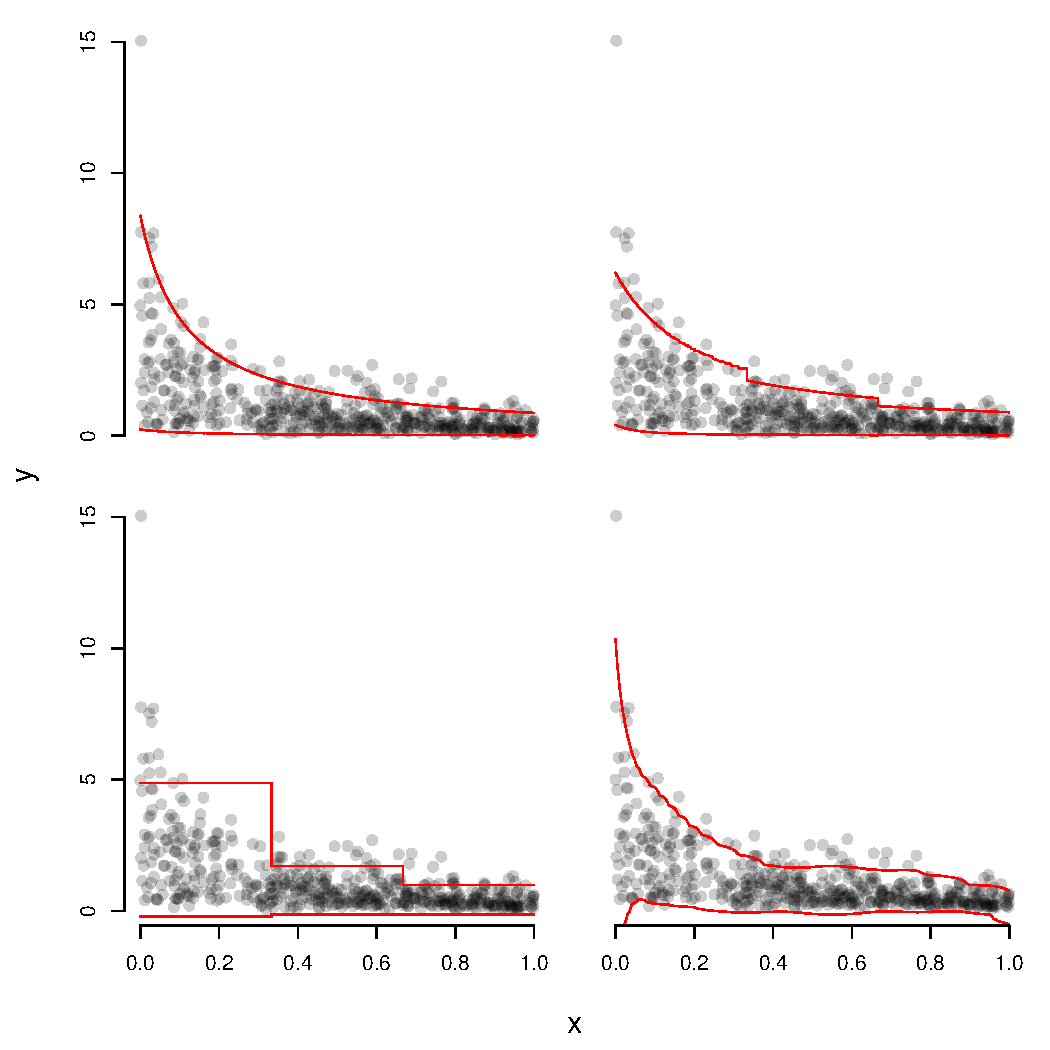
\includegraphics[width=\maxwidth]{figure/gammasimexample-1} 

\end{knitrout}
\end{center}
\caption{Sim setting: $n = 500$, shape = $2$, bins = $3$. 
  The regions are depicted as follows: 
    parametric conformal prediction region (top-left panel),
    nonparametric conformal prediction region (top-right panel),
    LSLW conformal prediction region (bottom-left panel),
    HD prediction region (bottom-right panel).}
\label{Fig:plots}
\end{figure}

All of the presented prediction regions exhibit close to finite-sample 
marginal validity and local validity with respect to bining.  However, 
the LSLW conformal prediction region and the HD prediction region do not 
exhibit finite-sample local validity in the second bin and the HD prediction 
region does not quite possess finite-sample marginal validity.  The parametric 
conformal prediction region is smallest in size with an estimated area of 
2.20.  The HD prediction region is a close second with an estimated area of 
2.21.  LSLW conformal prediction region has an estimated area of 2.57 and 
The nonparametric conformal prediction region has an estimated area of 2.69.  
Under correct model specification, the parametric conformal prediction 
region is similar in performance to that of the highest density prediction 
region.


\begin{knitrout}
\definecolor{shadecolor}{rgb}{0.969, 0.969, 0.969}\color{fgcolor}\begin{kframe}
\begin{alltt}
\hlcom{## parametric conformal prediction region}
\hlcom{# estimated area}
\hlkwd{mean}\hlstd{(}\hlkwd{apply}\hlstd{(paraCI,} \hlnum{1}\hlstd{, diff))}
\end{alltt}
\begin{verbatim}
## [1] 2.198495
\end{verbatim}
\begin{alltt}
\hlcom{# local coverage}
\hlstd{p} \hlkwb{<-} \hlkwd{length}\hlstd{(beta)} \hlopt{-} \hlnum{1}
\hlkwd{local.coverage}\hlstd{(}\hlkwc{region} \hlstd{= paraCI,} \hlkwc{data} \hlstd{= data.readme,} \hlkwc{d} \hlstd{= p,}
  \hlkwc{bins} \hlstd{= bins,} \hlkwc{at.data} \hlstd{=} \hlstr{"TRUE"}\hlstd{)}
\end{alltt}
\begin{verbatim}
## [1] 0.9135802 0.9028571 0.9079755
\end{verbatim}
\begin{alltt}
\hlcom{# marginal coverage}
\hlkwd{local.coverage}\hlstd{(}\hlkwc{region} \hlstd{= paraCI,} \hlkwc{data} \hlstd{= data.readme,} \hlkwc{d} \hlstd{= p,}
  \hlkwc{bins} \hlstd{=} \hlnum{1}\hlstd{,} \hlkwc{at.data} \hlstd{=} \hlstr{"TRUE"}\hlstd{)}
\end{alltt}
\begin{verbatim}
## [1] 0.908
\end{verbatim}
\begin{alltt}
\hlcom{## nonparametric conformal prediction region}
\hlcom{# estimated area}
\hlstd{area.nonparametric} \hlkwb{<-} \hlkwa{function}\hlstd{(}\hlkwc{region}\hlstd{)\{}
  \hlkwa{if}\hlstd{(}\hlkwd{class}\hlstd{(region)} \hlopt{!=} \hlstr{"list"}\hlstd{)\{}
    \hlkwd{stop}\hlstd{(}\hlstr{"Only appropriate for nonparametric conformal prediction region"}\hlstd{)}
  \hlstd{\}}
  \hlstd{bins} \hlkwb{<-} \hlkwd{length}\hlstd{(region); wn} \hlkwb{<-} \hlnum{1} \hlopt{/} \hlstd{bins}
  \hlstd{area} \hlkwb{<-} \hlnum{0}
  \hlkwa{for}\hlstd{(i} \hlkwa{in} \hlnum{1}\hlopt{:}\hlstd{bins)\{}
    \hlstd{nonpar.region} \hlkwb{<-} \hlstd{region[[i]]}
    \hlstd{area} \hlkwb{<-} \hlstd{area} \hlopt{+} \hlstd{wn} \hlopt{*} \hlkwd{as.numeric}\hlstd{(}\hlkwd{rep}\hlstd{(}\hlkwd{c}\hlstd{(}\hlopt{-}\hlnum{1}\hlstd{,}\hlnum{1}\hlstd{),}
      \hlkwd{length}\hlstd{(nonpar.region)}\hlopt{/}\hlnum{2}\hlstd{)} \hlopt \hlstd{nonpar.region)}
  \hlstd{\}}
  \hlstd{area}
\hlstd{\}}
\hlkwd{area.nonparametric}\hlstd{(nonparaCI)}
\end{alltt}
\begin{verbatim}
## [1] 2.687667
\end{verbatim}
\begin{alltt}
\hlcom{# local coverage}
\hlkwd{local.coverage}\hlstd{(}\hlkwc{region} \hlstd{= nonparaCI,} \hlkwc{data} \hlstd{= data.readme,} \hlkwc{d} \hlstd{= p,}
  \hlkwc{nonparametric} \hlstd{=} \hlstr{"TRUE"}\hlstd{,} \hlkwc{bins} \hlstd{= bins,} \hlkwc{at.data} \hlstd{=} \hlstr{"TRUE"}\hlstd{)}
\end{alltt}
\begin{verbatim}
## [1] 0.9259259 0.9028571 0.9018405
\end{verbatim}
\begin{alltt}
\hlcom{# marginal coverage}
\hlkwd{local.coverage}\hlstd{(}\hlkwc{region} \hlstd{= nonparaCI,} \hlkwc{data} \hlstd{= data.readme,} \hlkwc{d} \hlstd{= p,}
  \hlkwc{nonparametric} \hlstd{=} \hlstr{"TRUE"}\hlstd{,} \hlkwc{bins} \hlstd{=} \hlnum{1}\hlstd{,} \hlkwc{at.data} \hlstd{=} \hlstr{"TRUE"}\hlstd{)}
\end{alltt}
\begin{verbatim}
## [1] 0.91
\end{verbatim}
\begin{alltt}
\hlcom{## LSLW conformal prediction region}
\hlcom{# estimated area}
\hlkwd{mean}\hlstd{(}\hlkwd{apply}\hlstd{(LSLW,} \hlnum{1}\hlstd{, diff))}
\end{alltt}
\begin{verbatim}
## [1] 2.563743
\end{verbatim}
\begin{alltt}
\hlcom{# local coverage}
\hlkwd{local.coverage}\hlstd{(}\hlkwc{region} \hlstd{= LSLW,} \hlkwc{data} \hlstd{= data.readme,} \hlkwc{d} \hlstd{= p,}
  \hlkwc{bins} \hlstd{= bins,} \hlkwc{at.data} \hlstd{=} \hlstr{"TRUE"}\hlstd{)}
\end{alltt}
\begin{verbatim}
## [1] 0.9197531 0.8914286 0.9509202
\end{verbatim}
\begin{alltt}
\hlcom{# marginal coverage}
\hlkwd{local.coverage}\hlstd{(}\hlkwc{region} \hlstd{= LSLW,} \hlkwc{data} \hlstd{= data.readme,} \hlkwc{d} \hlstd{= p,}
  \hlkwc{bins} \hlstd{=} \hlnum{1}\hlstd{,} \hlkwc{at.data} \hlstd{=} \hlstr{"TRUE"}\hlstd{)}
\end{alltt}
\begin{verbatim}
## [1] 0.92
\end{verbatim}
\begin{alltt}
\hlcom{## HD region}
\hlcom{# estimated area}
\hlkwd{mean}\hlstd{(}\hlkwd{apply}\hlstd{(HDCI,} \hlnum{1}\hlstd{, diff))}
\end{alltt}
\begin{verbatim}
## [1] 2.207619
\end{verbatim}
\begin{alltt}
\hlcom{# local coverage}
\hlkwd{local.coverage}\hlstd{(}\hlkwc{region} \hlstd{= HDCI,} \hlkwc{data} \hlstd{= data.readme,} \hlkwc{d} \hlstd{= p,}
  \hlkwc{bins} \hlstd{= bins,} \hlkwc{at.data} \hlstd{=} \hlstr{"TRUE"}\hlstd{)}
\end{alltt}
\begin{verbatim}
## [1] 0.9012346 0.8800000 0.9079755
\end{verbatim}
\begin{alltt}
\hlcom{# marginal coverage}
\hlkwd{local.coverage}\hlstd{(}\hlkwc{region} \hlstd{= HDCI,} \hlkwc{data} \hlstd{= data.readme,} \hlkwc{d} \hlstd{= p,}
  \hlkwc{bins} \hlstd{=} \hlnum{1}\hlstd{,} \hlkwc{at.data} \hlstd{=} \hlstr{"TRUE"}\hlstd{)}
\end{alltt}
\begin{verbatim}
## [1] 0.896
\end{verbatim}
\end{kframe}
\end{knitrout}


\section{Extension of the illustrative example from the README file}

In this extension we investigate the local coverage properties of five 
prediction regions, the four from the previous section and a least squares 
(LS) conformal prediction region without local weighting.  Local coverage is 
assessed via a Monte Carlo simulation of size $B = 50$.  At each iteration 
of this simulation a new dataset is generated under the same specifications 
as those in the README file.  We then compute the local coverage probabilities 
with respect to each bin and also approximate conditional coverage across $x$.  
We do not assess coverage properties directly at $x$ for all $x \in (0,1]$.  
This corresponds to the notion of conditional validity which cannot be 
achieved in tandem with an oracle estimation in finite sample settings when 
distributions are continuous \citep[Section 2.2]{lei2014distribution}.  
What we do instead is we assess local coverage with a binning in $x$ that is 
much finer than the binning that was used to create the misspecified 
parametric and nonparametric conformal prediction regions.  We form 25 bins 
of length 0.04. 


\subsection{Diagnostic measures}

In this section we describe the diagnostic measures that we will use to 
compare conformal prediction regions.
The specific diagnostics are 
prediction error at the observed data, 
area of the prediction region, 
finite-sample marginal coverage,
finite-sample local coverage with respec to binning, 
and 
finite-sample local conditional coverage.  

We will use a modification of average sum of squares error as our measure of 
prediction error.  Our prediction error will average the squared distances of 
observations outside of the prediction region to the closest boundary of the 
prediction region.  The average will be taken over all observations so that an 
observation that falls within the prediction region has an error of 0.  
More formally this prediction error is 
$$
  \text{prediciton error} 
    = n^{-1}\sum_{i=1}^n\indicator{Y_i \not\in \Copt(X_i)}
      \left(\min\{|Y_i - a_{i,1}|, |Y_i - b_{i,1}|, \ldots, 
      |Y_i - a_{i,m_i}|, |Y_i - b_{i,m_i}|\}\right)^2,
$$
where $a_{i,j}$ and $b_{i,j}$ are, respectively, the lower and upper 
boundaries of possible $j = 1, \ldots, m_i$ disjoint intervals forming 
the prediction region.  

The area of each prediction region will be estimated by the average of the 
upper boundary minus the lower boundary across observed $\X$, written as
$$ 
  \text{area} = n^{-1}\sum_{i=1}^n\sum_{j=1}^{m_i}(b_{i,j} - a_{i,j}).
$$
This estimate of area is appropriate in our simulations in which realiztions 
of the predictors are generated as $X \sim U(0,1)$.   

To assess finite-sample marginal validity we calculate the proportion of 
responses that fall within the prediction region.  To assess finite-sample 
local validity with respect to binning we first bin the predictor data and 
then, for each bin, we calculate the proportion of responses that fall 
within the prediciton region. The same procedure is used to assess 
finite-sample conditional validity, but we use a much finer binning regime 
than what was used to assess finite-sample local validity.  

The following function computes our estimate of prediction error at the 
observed data when the prediction region is not the nonparametric 
conformal prediction region.

\begin{knitrout}
\definecolor{shadecolor}{rgb}{0.969, 0.969, 0.969}\color{fgcolor}\begin{kframe}
\begin{alltt}
\hlstd{absolute.error} \hlkwb{<-} \hlkwa{function}\hlstd{(}\hlkwc{y}\hlstd{,} \hlkwc{region}\hlstd{,} \hlkwc{squared} \hlstd{=} \hlnum{TRUE}\hlstd{)\{}
  \hlstd{lwr} \hlkwb{<-} \hlstd{region[,} \hlnum{1}\hlstd{]}
  \hlstd{upr} \hlkwb{<-} \hlstd{region[,} \hlnum{2}\hlstd{]}
  \hlstd{index} \hlkwb{<-} \hlkwd{which}\hlstd{(}\hlopt{!}\hlstd{(lwr} \hlopt{<=} \hlstd{y} \hlopt{&} \hlstd{y} \hlopt{<=} \hlstd{upr))}
  \hlstd{out} \hlkwb{<-} \hlkwd{sum}\hlstd{(}\hlkwd{unlist}\hlstd{(}\hlkwd{lapply}\hlstd{(index,} \hlkwa{function}\hlstd{(}\hlkwc{j}\hlstd{)\{}
    \hlstd{error} \hlkwb{<-} \hlkwa{NULL}
    \hlkwa{if}\hlstd{(squared} \hlopt{==} \hlnum{FALSE}\hlstd{) error} \hlkwb{<-}
      \hlkwd{min}\hlstd{(}\hlkwd{abs}\hlstd{(y[j]} \hlopt{-} \hlstd{lwr[j]),} \hlkwd{abs}\hlstd{(y[j]} \hlopt{-} \hlstd{upr[j]))}
    \hlkwa{if}\hlstd{(squared} \hlopt{==} \hlnum{TRUE}\hlstd{) error} \hlkwb{<-}
      \hlstd{(}\hlkwd{min}\hlstd{(}\hlkwd{abs}\hlstd{(y[j]} \hlopt{-} \hlstd{lwr[j]),} \hlkwd{abs}\hlstd{(y[j]} \hlopt{-} \hlstd{upr[j])))}\hlopt{^}\hlnum{2}
    \hlstd{error}
  \hlstd{\})))} \hlopt{/} \hlkwd{length}\hlstd{(y)}
  \hlstd{out}
\hlstd{\}}
\end{alltt}
\end{kframe}
\end{knitrout}

The following function computes our estimate of prediction error at the 
observed data when the prediction region is the nonparametric conformal 
prediction region.

\begin{knitrout}
\definecolor{shadecolor}{rgb}{0.969, 0.969, 0.969}\color{fgcolor}\begin{kframe}
\begin{alltt}
\hlstd{absolute.error.nonparametric} \hlkwb{<-} \hlkwa{function}\hlstd{(}\hlkwc{data}\hlstd{,} \hlkwc{region}\hlstd{,}
  \hlkwc{squared} \hlstd{=} \hlnum{TRUE}\hlstd{)\{}
  \hlstd{n} \hlkwb{<-} \hlkwd{nrow}\hlstd{(data)}
  \hlstd{n.bins.region} \hlkwb{<-} \hlkwd{length}\hlstd{(region)}
  \hlstd{d} \hlkwb{<-} \hlkwd{ncol}\hlstd{(data)} \hlopt{-} \hlnum{1}
  \hlstd{x} \hlkwb{<-} \hlkwd{as.matrix}\hlstd{(data[,}\hlnum{1}\hlopt{:}\hlstd{d} \hlopt{+} \hlnum{1}\hlstd{],} \hlkwc{col} \hlstd{= d)}
  \hlstd{index.bins.region} \hlkwb{<-} \hlkwd{find.index}\hlstd{(x,} \hlkwc{wn} \hlstd{=} \hlnum{1}\hlopt{/}\hlstd{n.bins.region,} \hlkwc{d} \hlstd{= d)}
  \hlstd{y} \hlkwb{<-} \hlstd{data[,} \hlnum{1}\hlstd{]}
  \hlstd{area} \hlkwb{<-} \hlnum{0}
  \hlkwa{for}\hlstd{(j} \hlkwa{in} \hlnum{1}\hlopt{:}\hlstd{n)\{}
    \hlstd{index.j} \hlkwb{<-} \hlkwd{which}\hlstd{(index.bins.region} \hlopt{==} \hlstd{j)}
    \hlstd{error} \hlkwb{<-} \hlkwd{c}\hlstd{(y[j]} \hlopt{-} \hlstd{region[[index.bins.region[j]]])}
    \hlstd{index} \hlkwb{<-} \hlnum{0}
    \hlkwa{if}\hlstd{(}\hlkwd{any}\hlstd{(error} \hlopt{>} \hlnum{0}\hlstd{)) index} \hlkwb{<-} \hlkwd{max}\hlstd{(}\hlkwd{which}\hlstd{(error} \hlopt{>} \hlnum{0}\hlstd{))}
    \hlkwa{if}\hlstd{(index} \hlopt \hlnum{2} \hlopt{==} \hlnum{0}\hlstd{)\{}
      \hlkwa{if}\hlstd{(squared} \hlopt{==} \hlnum{FALSE}\hlstd{) area} \hlkwb{<-}
        \hlstd{area} \hlopt{+} \hlkwd{min}\hlstd{(}\hlkwd{abs}\hlstd{(error))} \hlopt{/} \hlstd{n}
      \hlkwa{if}\hlstd{(squared} \hlopt{==} \hlnum{TRUE}\hlstd{) area} \hlkwb{<-}
        \hlstd{area} \hlopt{+} \hlkwd{min}\hlstd{(}\hlkwd{abs}\hlstd{(error))}\hlopt{^}\hlnum{2} \hlopt{/} \hlstd{n}
    \hlstd{\}}
  \hlstd{\}}
  \hlstd{area}
\hlstd{\}}
\end{alltt}
\end{kframe}
\end{knitrout}

Our Monte Carlo simulator follows. This function computes all of the 
dignostics and local coverage probabilities for each prediction region 
for every generated dataset.

\begin{knitrout}
\definecolor{shadecolor}{rgb}{0.969, 0.969, 0.969}\color{fgcolor}\begin{kframe}
\begin{alltt}
\hlstd{gamma.simulator} \hlkwb{<-} \hlkwa{function}\hlstd{(}\hlkwc{n} \hlstd{=} \hlnum{500}\hlstd{,} \hlkwc{alpha} \hlstd{=} \hlnum{0.10}\hlstd{,} \hlkwc{beta}\hlstd{,} \hlkwc{bins} \hlstd{=} \hlnum{3}\hlstd{,}
  \hlkwc{family} \hlstd{=} \hlstr{"Gamma"}\hlstd{,} \hlkwc{link} \hlstd{=} \hlstr{"inverse"}\hlstd{,} \hlkwc{shape} \hlstd{=} \hlnum{2}\hlstd{,}
  \hlkwc{parametric} \hlstd{=} \hlnum{TRUE}\hlstd{,} \hlkwc{nonparametric} \hlstd{=} \hlnum{TRUE}\hlstd{,}
  \hlkwc{LS} \hlstd{=} \hlnum{TRUE}\hlstd{,} \hlkwc{LSLW} \hlstd{=} \hlnum{TRUE}\hlstd{,} \hlkwc{HD} \hlstd{=} \hlnum{TRUE}\hlstd{,} \hlkwc{cores} \hlstd{=} \hlnum{6}\hlstd{)\{}

  \hlcom{## in this univariate problem, p and d are the same}
  \hlstd{p} \hlkwb{<-} \hlstd{d} \hlkwb{<-} \hlkwd{length}\hlstd{(beta)} \hlopt{-} \hlnum{1}
  \hlstd{x} \hlkwb{<-} \hlkwd{matrix}\hlstd{(}\hlkwd{runif}\hlstd{(n),} \hlkwc{ncol} \hlstd{= p)}
  \hlstd{y} \hlkwb{<-} \hlkwd{rep}\hlstd{(}\hlnum{0}\hlstd{,n)}
  \hlstd{data} \hlkwb{<-} \hlkwa{NULL}

  \hlcom{## set up partition}
  \hlkwa{if}\hlstd{(}\hlkwd{class}\hlstd{(bins)} \hlopt{==} \hlstr{"NULL"}\hlstd{)\{}
    \hlstd{wn} \hlkwb{<-} \hlkwd{min}\hlstd{(}\hlnum{1}\hlopt{/} \hlkwd{floor}\hlstd{(}\hlnum{1} \hlopt{/} \hlstd{(}\hlkwd{log}\hlstd{(n)}\hlopt{/}\hlstd{n)}\hlopt{^}\hlstd{(}\hlnum{1}\hlopt{/}\hlstd{(d}\hlopt{+}\hlnum{3}\hlstd{))),} \hlnum{1}\hlopt{/}\hlnum{2}\hlstd{)}
    \hlstd{bins} \hlkwb{<-} \hlnum{1} \hlopt{/} \hlstd{wn}
  \hlstd{\}}

  \hlcom{## generate the data (has functionality for different }
  \hlcom{## families and link functions)}
  \hlkwa{if}\hlstd{(family} \hlopt{==} \hlstr{"Gamma"}\hlstd{)\{}
    \hlkwa{if}\hlstd{(link} \hlopt{==} \hlstr{"identity"}\hlstd{)\{}
      \hlstd{rate} \hlkwb{<-} \hlstd{(}\hlnum{1} \hlopt{/} \hlstd{(}\hlkwd{cbind}\hlstd{(}\hlnum{1}\hlstd{, x)} \hlopt \hlstd{beta))} \hlopt{*} \hlstd{shape}
      \hlstd{y} \hlkwb{<-} \hlkwd{rgamma}\hlstd{(}\hlkwc{n} \hlstd{= n,} \hlkwc{shape} \hlstd{= shape,} \hlkwc{rate} \hlstd{= rate)}
      \hlstd{y} \hlkwb{<-} \hlstd{y} \hlopt{/} \hlkwd{sd}\hlstd{(y)}
      \hlstd{data} \hlkwb{<-} \hlkwd{data.frame}\hlstd{(}\hlkwc{y} \hlstd{= y,} \hlkwc{x} \hlstd{= x)}
      \hlkwd{colnames}\hlstd{(data)[}\hlnum{2}\hlopt{:}\hlstd{(p}\hlopt{+}\hlnum{1}\hlstd{)]} \hlkwb{<-} \hlkwd{paste}\hlstd{(}\hlstr{"x"}\hlstd{,} \hlnum{1}\hlopt{:}\hlstd{p,} \hlkwc{sep} \hlstd{=} \hlstr{""}\hlstd{)}
    \hlstd{\}}
    \hlkwa{if}\hlstd{(link} \hlopt{==} \hlstr{"inverse"}\hlstd{)\{}
      \hlstd{rate} \hlkwb{<-} \hlstd{(}\hlkwd{cbind}\hlstd{(}\hlnum{1}\hlstd{, x)} \hlopt \hlstd{beta)} \hlopt{*} \hlstd{shape}
      \hlstd{y} \hlkwb{<-} \hlkwd{rgamma}\hlstd{(}\hlkwc{n} \hlstd{= n,} \hlkwc{shape} \hlstd{= shape,} \hlkwc{rate} \hlstd{= rate)}
      \hlstd{y} \hlkwb{<-} \hlstd{y} \hlopt{/} \hlkwd{sd}\hlstd{(y)}
      \hlstd{data} \hlkwb{<-} \hlkwd{data.frame}\hlstd{(}\hlkwc{y} \hlstd{= y,} \hlkwc{x} \hlstd{= x)}
      \hlkwd{colnames}\hlstd{(data)[}\hlnum{2}\hlopt{:}\hlstd{(p}\hlopt{+}\hlnum{1}\hlstd{)]} \hlkwb{<-} \hlkwd{paste}\hlstd{(}\hlstr{"x"}\hlstd{,} \hlnum{1}\hlopt{:}\hlstd{p,} \hlkwc{sep} \hlstd{=} \hlstr{""}\hlstd{)}
    \hlstd{\}}
    \hlkwa{if}\hlstd{(link} \hlopt{==} \hlstr{"log"}\hlstd{)\{}
      \hlstd{rate} \hlkwb{<-} \hlstd{(}\hlnum{1} \hlopt{/} \hlkwd{exp}\hlstd{(}\hlkwd{cbind}\hlstd{(}\hlnum{1}\hlstd{, x)} \hlopt \hlstd{beta))} \hlopt{*} \hlstd{shape}
      \hlstd{y} \hlkwb{<-} \hlkwd{rgamma}\hlstd{(}\hlkwc{n} \hlstd{= n,} \hlkwc{shape} \hlstd{= shape,} \hlkwc{rate} \hlstd{= rate)}
      \hlstd{y} \hlkwb{<-} \hlstd{y} \hlopt{/} \hlkwd{sd}\hlstd{(y)}
      \hlstd{data} \hlkwb{<-} \hlkwd{data.frame}\hlstd{(}\hlkwc{y} \hlstd{= y,} \hlkwc{x} \hlstd{= x)}
      \hlkwd{colnames}\hlstd{(data)[}\hlnum{2}\hlopt{:}\hlstd{(p}\hlopt{+}\hlnum{1}\hlstd{)]} \hlkwb{<-} \hlkwd{paste}\hlstd{(}\hlstr{"x"}\hlstd{,} \hlnum{1}\hlopt{:}\hlstd{p,} \hlkwc{sep} \hlstd{=} \hlstr{""}\hlstd{)}
    \hlstd{\}}
  \hlstd{\}}

  \hlkwa{if}\hlstd{(family} \hlopt{==} \hlstr{"gaussian"}\hlstd{)\{}
    \hlstd{mu} \hlkwb{<-} \hlkwd{cbind}\hlstd{(}\hlnum{1}\hlstd{, x)} \hlopt \hlstd{beta}
    \hlstd{y} \hlkwb{<-} \hlkwd{rnorm}\hlstd{(}\hlkwc{n} \hlstd{= n,} \hlkwc{mean} \hlstd{= mu,} \hlkwc{sd} \hlstd{= sd)}
    \hlstd{data} \hlkwb{<-} \hlkwd{data.frame}\hlstd{(}\hlkwc{y} \hlstd{= y,} \hlkwc{x} \hlstd{= x)}
    \hlkwd{colnames}\hlstd{(data)[}\hlnum{2}\hlopt{:}\hlstd{(p}\hlopt{+}\hlnum{1}\hlstd{)]} \hlkwb{<-} \hlkwd{paste}\hlstd{(}\hlstr{"x"}\hlstd{,} \hlnum{1}\hlopt{:}\hlstd{p,} \hlkwc{sep} \hlstd{=} \hlstr{""}\hlstd{)}
  \hlstd{\}}

  \hlkwa{if}\hlstd{(family} \hlopt{==} \hlstr{"inverse.gaussian"}\hlstd{)\{}
    \hlstd{mu} \hlkwb{=} \hlnum{1} \hlopt{/} \hlkwd{sqrt}\hlstd{(}\hlkwd{cbind}\hlstd{(}\hlnum{1}\hlstd{, x)} \hlopt \hlstd{beta)}
    \hlstd{y} \hlkwb{<-} \hlkwd{rinvgauss}\hlstd{(}\hlkwc{n} \hlstd{= n,} \hlkwc{mean} \hlstd{= mu)}
    \hlstd{y} \hlkwb{<-} \hlstd{y} \hlopt{/} \hlkwd{sd}\hlstd{(y)}
    \hlstd{data} \hlkwb{<-} \hlkwd{data.frame}\hlstd{(}\hlkwc{y} \hlstd{= y,} \hlkwc{x} \hlstd{= x)}
    \hlkwd{colnames}\hlstd{(data)[}\hlnum{2}\hlopt{:}\hlstd{(p}\hlopt{+}\hlnum{1}\hlstd{)]} \hlkwb{<-} \hlkwd{paste}\hlstd{(}\hlstr{"x"}\hlstd{,} \hlnum{1}\hlopt{:}\hlstd{p,} \hlkwc{sep} \hlstd{=} \hlstr{""}\hlstd{)}
  \hlstd{\}}

  \hlcom{## fit the Gamma regression model}
  \hlstd{fit} \hlkwb{<-} \hlkwd{glm}\hlstd{(y} \hlopt{~} \hlstd{x1,} \hlkwc{family} \hlstd{=} \hlstr{"Gamma"}\hlstd{,} \hlkwc{data} \hlstd{= data)}
  \hlstd{paraCI} \hlkwb{<-} \hlstd{nonparaCI} \hlkwb{<-} \hlstd{LSCI} \hlkwb{<-} \hlstd{LSLWCI} \hlkwb{<-} \hlstd{HDCI} \hlkwb{<-} \hlkwa{NULL}
  \hlstd{formula} \hlkwb{<-} \hlstd{fit}\hlopt{$}\hlstd{formula}
  \hlstd{newdata} \hlkwb{<-} \hlstd{data}
  \hlstd{respname} \hlkwb{<-} \hlkwd{all.vars}\hlstd{(formula)[}\hlnum{1}\hlstd{]}
  \hlstd{newdata} \hlkwb{<-} \hlstd{newdata[,} \hlopt{!}\hlstd{(}\hlkwd{colnames}\hlstd{(data)} \hlopt \hlstd{respname)]}
  \hlstd{newdata} \hlkwb{<-} \hlkwd{as.matrix}\hlstd{(newdata)}

  \hlcom{## obtain the prediction regions}
  \hlkwa{if}\hlstd{(parametric)\{}
    \hlstd{cpred} \hlkwb{<-} \hlkwd{conformal.glm}\hlstd{(fit,} \hlkwc{parametric} \hlstd{=} \hlnum{TRUE}\hlstd{,}
      \hlkwc{nonparametric} \hlstd{=} \hlnum{FALSE}\hlstd{,} \hlkwc{alpha} \hlstd{= alpha,}
      \hlkwc{bins} \hlstd{= bins,} \hlkwc{cores} \hlstd{= cores)}
    \hlstd{paraCI} \hlkwb{<-} \hlstd{cpred}\hlopt{$}\hlstd{paraconformal}
  \hlstd{\}}
  \hlkwa{if}\hlstd{(nonparametric)\{}
    \hlstd{cpred} \hlkwb{<-} \hlkwd{conformal.glm}\hlstd{(fit,} \hlkwc{parametric} \hlstd{=} \hlnum{FALSE}\hlstd{,}
      \hlkwc{nonparametric} \hlstd{=} \hlnum{TRUE}\hlstd{,} \hlkwc{alpha} \hlstd{= alpha,}
      \hlkwc{bins} \hlstd{= bins,} \hlkwc{cores} \hlstd{= cores)}
    \hlstd{nonparaCI} \hlkwb{<-} \hlstd{cpred}\hlopt{$}\hlstd{nonparaconformal}
  \hlstd{\}}
  \hlkwa{if}\hlstd{(LS)\{}
    \hlstd{p1.tibs} \hlkwb{<-} \hlkwd{conformal.pred}\hlstd{(}\hlkwc{x} \hlstd{=} \hlkwd{cbind}\hlstd{(x,x}\hlopt{^}\hlnum{2}\hlstd{,x}\hlopt{^}\hlnum{3}\hlstd{),} \hlkwc{y} \hlstd{= y,}
      \hlkwc{x0} \hlstd{=} \hlkwd{cbind}\hlstd{(x,x}\hlopt{^}\hlnum{2}\hlstd{,x}\hlopt{^}\hlnum{3}\hlstd{),}
      \hlkwc{train.fun} \hlstd{= train.fun,} \hlkwc{predict.fun} \hlstd{= predict.fun,}
      \hlkwc{alpha} \hlstd{= alpha)}
    \hlstd{LSCI} \hlkwb{<-} \hlkwd{cbind}\hlstd{(p1.tibs}\hlopt{$}\hlstd{lo, p1.tibs}\hlopt{$}\hlstd{up)}
  \hlstd{\}}
  \hlkwa{if}\hlstd{(LSLW)\{}
    \hlstd{cubic.model} \hlkwb{<-} \hlkwd{lm}\hlstd{(y} \hlopt{~} \hlstd{x} \hlopt{+} \hlkwd{I}\hlstd{(x}\hlopt{^}\hlnum{2}\hlstd{)} \hlopt{+} \hlkwd{I}\hlstd{(x}\hlopt{^}\hlnum{3}\hlstd{))}
    \hlstd{abs.resid} \hlkwb{<-} \hlkwd{abs}\hlstd{(cubic.model}\hlopt{$}\hlstd{resid)}
    \hlstd{smooth.call} \hlkwb{<-} \hlkwd{smooth.spline}\hlstd{(x, abs.resid,}
      \hlkwc{nknots} \hlstd{=} \hlnum{10}\hlstd{)}
    \hlstd{lambda} \hlkwb{<-} \hlstd{smooth.call}\hlopt{$}\hlstd{lambda}
    \hlstd{df} \hlkwb{<-} \hlstd{smooth.call}\hlopt{$}\hlstd{df}
    \hlstd{mad.train.fun} \hlkwb{<-} \hlkwa{function}\hlstd{(}\hlkwc{x}\hlstd{,} \hlkwc{y}\hlstd{,} \hlkwc{out} \hlstd{=} \hlkwa{NULL}\hlstd{)\{}
      \hlkwd{smooth.spline}\hlstd{(x[,} \hlnum{1}\hlstd{], y,} \hlkwc{lambda} \hlstd{= lambda,}
      \hlkwc{df} \hlstd{= df,} \hlkwc{nknots} \hlstd{=} \hlnum{10}\hlstd{)}
    \hlstd{\}}
    \hlstd{p2.tibs} \hlkwb{<-} \hlkwd{conformal.pred}\hlstd{(}\hlkwc{x} \hlstd{=} \hlkwd{cbind}\hlstd{(x,x}\hlopt{^}\hlnum{2}\hlstd{,x}\hlopt{^}\hlnum{3}\hlstd{),} \hlkwc{y} \hlstd{= y,}
      \hlkwc{x0} \hlstd{=} \hlkwd{cbind}\hlstd{(x,x}\hlopt{^}\hlnum{2}\hlstd{,x}\hlopt{^}\hlnum{3}\hlstd{),}
      \hlkwc{train.fun} \hlstd{= train.fun,} \hlkwc{predict.fun} \hlstd{= predict.fun,}
      \hlkwc{mad.train.fun} \hlstd{= mad.train.fun,}
      \hlkwc{mad.predict.fun} \hlstd{= mad.predict.fun,}
      \hlkwc{alpha} \hlstd{= alpha)}
    \hlstd{LSLWCI} \hlkwb{<-} \hlkwd{cbind}\hlstd{(p2.tibs}\hlopt{$}\hlstd{lo, p2.tibs}\hlopt{$}\hlstd{up)}
  \hlstd{\}}
  \hlkwa{if}\hlstd{(HD)\{}
    \hlstd{betaMLE} \hlkwb{<-} \hlkwd{coefficients}\hlstd{(fit)}
    \hlstd{shapeMLE} \hlkwb{<-} \hlkwd{as.numeric}\hlstd{(}\hlkwd{gamma.shape}\hlstd{(fit)[}\hlnum{1}\hlstd{])}
    \hlstd{rateMLE} \hlkwb{<-} \hlkwd{cbind}\hlstd{(}\hlnum{1}\hlstd{, newdata)} \hlopt \hlstd{betaMLE} \hlopt{*} \hlstd{shapeMLE}
    \hlstd{HDCI} \hlkwb{<-} \hlkwd{do.call}\hlstd{(rbind,} \hlkwd{lapply}\hlstd{(}\hlnum{1}\hlopt{:}\hlkwd{nrow}\hlstd{(newdata),} \hlkwa{function}\hlstd{(}\hlkwc{j}\hlstd{)\{}
      \hlkwd{hdi}\hlstd{(qgamma,} \hlnum{1} \hlopt{-} \hlstd{alpha,} \hlkwc{shape} \hlstd{= shapeMLE,} \hlkwc{rate} \hlstd{= rateMLE[j,} \hlnum{1}\hlstd{])}
    \hlstd{\}))}
  \hlstd{\}}

  \hlcom{## local coverage prediction regions}
  \hlstd{output.parametric} \hlkwb{<-} \hlstd{output.nonparametric} \hlkwb{<-}
    \hlstd{output.LS} \hlkwb{<-} \hlstd{output.LSLW} \hlkwb{<-} \hlstd{output.HD} \hlkwb{<-} \hlkwd{rep}\hlstd{(}\hlnum{NA}\hlstd{, bins} \hlopt{+} \hlnum{1}\hlstd{)}
  \hlkwa{if}\hlstd{(parametric)\{}
    \hlstd{marginal.parametric} \hlkwb{<-} \hlkwd{local.coverage}\hlstd{(}\hlkwc{region} \hlstd{= paraCI,}
      \hlkwc{data} \hlstd{= data,} \hlkwc{d} \hlstd{= p,} \hlkwc{bins} \hlstd{=} \hlnum{1}\hlstd{,} \hlkwc{at.data} \hlstd{=} \hlstr{"TRUE"}\hlstd{)}
    \hlstd{local.parametric} \hlkwb{<-} \hlkwd{local.coverage}\hlstd{(}\hlkwc{region} \hlstd{= paraCI,}
      \hlkwc{data} \hlstd{= data,} \hlkwc{d} \hlstd{= p,} \hlkwc{bins} \hlstd{= bins,} \hlkwc{at.data} \hlstd{=} \hlstr{"TRUE"}\hlstd{)}
    \hlstd{local.inx.parametric} \hlkwb{<-} \hlkwd{local.coverage}\hlstd{(}\hlkwc{region} \hlstd{= paraCI,}
      \hlkwc{data} \hlstd{= data,} \hlkwc{d} \hlstd{= p,} \hlkwc{bins} \hlstd{=} \hlnum{25}\hlstd{,} \hlkwc{at.data} \hlstd{=} \hlstr{"TRUE"}\hlstd{)}
    \hlstd{output.parametric} \hlkwb{<-} \hlkwd{c}\hlstd{(marginal.parametric, local.parametric,}
      \hlstd{local.inx.parametric,}
      \hlkwd{mean}\hlstd{(}\hlkwd{apply}\hlstd{(paraCI,} \hlnum{1}\hlstd{, diff)),}
      \hlkwd{absolute.error}\hlstd{(}\hlkwc{y} \hlstd{= y,} \hlkwc{region} \hlstd{= paraCI))}
  \hlstd{\}}
  \hlkwa{if}\hlstd{(nonparametric)\{}
    \hlstd{marginal.nonparametric} \hlkwb{<-} \hlkwd{local.coverage}\hlstd{(}\hlkwc{region} \hlstd{= nonparaCI,}
      \hlkwc{nonparametric} \hlstd{=} \hlstr{"TRUE"}\hlstd{,} \hlkwc{data} \hlstd{= data,} \hlkwc{d} \hlstd{= p,} \hlkwc{bins} \hlstd{=} \hlnum{1}\hlstd{,}
      \hlkwc{at.data} \hlstd{=} \hlstr{"TRUE"}\hlstd{)}
    \hlstd{local.nonparametric} \hlkwb{<-} \hlkwd{local.coverage}\hlstd{(}\hlkwc{region} \hlstd{= nonparaCI,}
      \hlkwc{nonparametric} \hlstd{=} \hlstr{"TRUE"}\hlstd{,} \hlkwc{data} \hlstd{= data,} \hlkwc{d} \hlstd{= p,} \hlkwc{bins} \hlstd{= bins,}
      \hlkwc{at.data} \hlstd{=} \hlstr{"TRUE"}\hlstd{)}
    \hlstd{local.inx.nonparametric} \hlkwb{<-} \hlkwd{local.coverage}\hlstd{(}\hlkwc{region} \hlstd{= nonparaCI,}
      \hlkwc{nonparametric} \hlstd{=} \hlstr{"TRUE"}\hlstd{,} \hlkwc{data} \hlstd{= data,} \hlkwc{d} \hlstd{= p,} \hlkwc{bins} \hlstd{=} \hlnum{25}\hlstd{,}
      \hlkwc{at.data} \hlstd{=} \hlstr{"TRUE"}\hlstd{)}
    \hlstd{output.nonparametric} \hlkwb{<-}
      \hlkwd{c}\hlstd{(marginal.nonparametric, local.nonparametric,}
        \hlstd{local.inx.nonparametric,}
        \hlkwd{area.nonparametric}\hlstd{(nonparaCI),}
        \hlkwd{absolute.error.nonparametric}\hlstd{(}\hlkwc{data} \hlstd{= data,}
          \hlkwc{region} \hlstd{= nonparaCI))}
  \hlstd{\}}
  \hlkwa{if}\hlstd{(LS)\{}
    \hlstd{marginal.LS} \hlkwb{<-} \hlkwd{local.coverage}\hlstd{(}\hlkwc{region} \hlstd{= LSCI,}
      \hlkwc{data} \hlstd{= data,} \hlkwc{d} \hlstd{= p,} \hlkwc{bins} \hlstd{=} \hlnum{1}\hlstd{,} \hlkwc{at.data} \hlstd{=} \hlstr{"TRUE"}\hlstd{)}
    \hlstd{local.LS} \hlkwb{<-} \hlkwd{local.coverage}\hlstd{(}\hlkwc{region} \hlstd{= LSCI,}
      \hlkwc{data} \hlstd{= data,} \hlkwc{d} \hlstd{= p,} \hlkwc{bins} \hlstd{= bins,} \hlkwc{at.data} \hlstd{=} \hlstr{"TRUE"}\hlstd{)}
    \hlstd{local.inx.LS} \hlkwb{<-} \hlkwd{local.coverage}\hlstd{(}\hlkwc{region} \hlstd{= LSCI,}
      \hlkwc{data} \hlstd{= data,} \hlkwc{d} \hlstd{= p,} \hlkwc{bins} \hlstd{=} \hlnum{25}\hlstd{,} \hlkwc{at.data} \hlstd{=} \hlstr{"TRUE"}\hlstd{)}
    \hlstd{output.LS} \hlkwb{<-} \hlkwd{c}\hlstd{(marginal.LS, local.LS, local.inx.LS,}
      \hlkwd{mean}\hlstd{(}\hlkwd{apply}\hlstd{(LSCI,} \hlnum{1}\hlstd{, diff)),}
      \hlkwd{absolute.error}\hlstd{(}\hlkwc{y} \hlstd{= y,} \hlkwc{region} \hlstd{= LSCI))}
  \hlstd{\}}
  \hlkwa{if}\hlstd{(LSLW)\{}
    \hlstd{marginal.LSLW} \hlkwb{<-} \hlkwd{local.coverage}\hlstd{(}\hlkwc{region} \hlstd{= LSLWCI,}
      \hlkwc{data} \hlstd{= data,} \hlkwc{d} \hlstd{= p,} \hlkwc{bins} \hlstd{=} \hlnum{1}\hlstd{,} \hlkwc{at.data} \hlstd{=} \hlstr{"TRUE"}\hlstd{)}
    \hlstd{local.LSLW} \hlkwb{<-} \hlkwd{local.coverage}\hlstd{(}\hlkwc{region} \hlstd{= LSLWCI,}
      \hlkwc{data} \hlstd{= data,} \hlkwc{d} \hlstd{= p,} \hlkwc{bins} \hlstd{= bins,} \hlkwc{at.data} \hlstd{=} \hlstr{"TRUE"}\hlstd{)}
    \hlstd{local.inx.LSLW} \hlkwb{<-} \hlkwd{local.coverage}\hlstd{(}\hlkwc{region} \hlstd{= LSLWCI,}
      \hlkwc{data} \hlstd{= data,} \hlkwc{d} \hlstd{= p,} \hlkwc{bins} \hlstd{=} \hlnum{25}\hlstd{,} \hlkwc{at.data} \hlstd{=} \hlstr{"TRUE"}\hlstd{)}
    \hlstd{output.LSLW} \hlkwb{<-} \hlkwd{c}\hlstd{(marginal.LSLW, local.LSLW, local.inx.LSLW,}
      \hlkwd{mean}\hlstd{(}\hlkwd{apply}\hlstd{(LSLWCI,} \hlnum{1}\hlstd{, diff)),}
      \hlkwd{absolute.error}\hlstd{(}\hlkwc{y} \hlstd{= y,} \hlkwc{region} \hlstd{= LSLWCI))}
  \hlstd{\}}
  \hlkwa{if}\hlstd{(HD)\{}
    \hlstd{marginal.HD} \hlkwb{<-} \hlkwd{local.coverage}\hlstd{(}\hlkwc{region} \hlstd{= HDCI,}
      \hlkwc{data} \hlstd{= data,} \hlkwc{d} \hlstd{= p,} \hlkwc{bins} \hlstd{=} \hlnum{1}\hlstd{,} \hlkwc{at.data} \hlstd{=} \hlstr{"TRUE"}\hlstd{)}
    \hlstd{local.HD} \hlkwb{<-} \hlkwd{local.coverage}\hlstd{(}\hlkwc{region} \hlstd{= HDCI,}
      \hlkwc{data} \hlstd{= data,} \hlkwc{d} \hlstd{= p,} \hlkwc{bins} \hlstd{= bins,} \hlkwc{at.data} \hlstd{=} \hlstr{"TRUE"}\hlstd{)}
    \hlstd{local.inx.HD} \hlkwb{<-} \hlkwd{local.coverage}\hlstd{(}\hlkwc{region} \hlstd{= HDCI,}
      \hlkwc{data} \hlstd{= data,} \hlkwc{d} \hlstd{= p,} \hlkwc{bins} \hlstd{=} \hlnum{25}\hlstd{,} \hlkwc{at.data} \hlstd{=} \hlstr{"TRUE"}\hlstd{)}
    \hlstd{output.HD} \hlkwb{<-} \hlkwd{c}\hlstd{(marginal.HD, local.HD, local.inx.HD,}
      \hlkwd{mean}\hlstd{(}\hlkwd{apply}\hlstd{(HDCI,} \hlnum{1}\hlstd{, diff)),}
      \hlkwd{absolute.error}\hlstd{(}\hlkwc{y} \hlstd{= y,} \hlkwc{region} \hlstd{= HDCI))}
  \hlstd{\}}

  \hlstd{output} \hlkwb{<-} \hlkwd{list}\hlstd{(}\hlkwc{output.parametric} \hlstd{= output.parametric,}
    \hlkwc{output.nonparametric} \hlstd{= output.nonparametric,}
    \hlkwc{output.LS} \hlstd{= output.LS,}
    \hlkwc{output.LSLW} \hlstd{= output.LSLW,}
    \hlkwc{output.HD} \hlstd{= output.HD)}
  \hlstd{output}

\hlstd{\}}
\end{alltt}
\end{kframe}
\end{knitrout}

The following performs our Monte Carlo simulation with $B = 50$ iterations. 

\begin{knitrout}
\definecolor{shadecolor}{rgb}{0.969, 0.969, 0.969}\color{fgcolor}\begin{kframe}
\begin{alltt}
\hlstd{B} \hlkwb{<-} \hlnum{50}
\hlkwd{system.time}\hlstd{(local.500.3.2} \hlkwb{<-} \hlkwd{do.call}\hlstd{(cbind,} \hlkwd{lapply}\hlstd{(}\hlnum{1}\hlopt{:}\hlstd{B,}
  \hlkwc{FUN} \hlstd{=} \hlkwa{function}\hlstd{(}\hlkwc{j}\hlstd{)\{}
    \hlkwd{unlist}\hlstd{(}\hlkwd{gamma.simulator}\hlstd{(}\hlkwc{beta} \hlstd{= beta))}
\hlstd{\})))}
\end{alltt}
\begin{verbatim}
##      user    system   elapsed 
## 13157.579    25.694  6385.948
\end{verbatim}
\end{kframe}
\end{knitrout}

\begin{knitrout}
\definecolor{shadecolor}{rgb}{0.969, 0.969, 0.969}\color{fgcolor}\begin{kframe}
\begin{alltt}
\hlstd{local.gamma.500.3.2} \hlkwb{<-} \hlkwd{cbind}\hlstd{(}
  \hlkwd{rowMeans}\hlstd{(local.500.3.2,} \hlkwc{na.rm} \hlstd{=} \hlnum{TRUE}\hlstd{),}
  \hlkwd{apply}\hlstd{(local.500.3.2,} \hlnum{1}\hlstd{,}
  \hlkwc{FUN} \hlstd{=} \hlkwa{function}\hlstd{(}\hlkwc{x}\hlstd{)\{}
    \hlstd{sds} \hlkwb{<-} \hlkwd{sd}\hlstd{(x,} \hlkwc{na.rm} \hlstd{=} \hlnum{TRUE}\hlstd{)}
    \hlstd{lengths} \hlkwb{<-} \hlkwd{length}\hlstd{(}\hlkwd{which}\hlstd{(}\hlopt{!}\hlkwd{is.na}\hlstd{(x)))}
    \hlstd{sds} \hlopt{/} \hlkwd{sqrt}\hlstd{(lengths)}
  \hlstd{\}))}

\hlkwd{options}\hlstd{(}\hlkwc{scipen} \hlstd{=} \hlnum{999}\hlstd{)}
\hlstd{local.gamma.500.3.2[,} \hlnum{1}\hlstd{]} \hlkwb{<-} \hlkwd{round}\hlstd{(local.gamma.500.3.2[,} \hlnum{1}\hlstd{],} \hlnum{3}\hlstd{)}
\hlstd{local.gamma.500.3.2[,} \hlnum{2}\hlstd{]} \hlkwb{<-} \hlkwd{round}\hlstd{(local.gamma.500.3.2[,} \hlnum{2}\hlstd{],} \hlnum{4}\hlstd{)}
\end{alltt}
\end{kframe}
\end{knitrout}


%Describe the table
Diagnostics for each of the five prediction regions are given in Table 1 and 
Figure~\ref{Fig:coverageinx500.3}.  We see that the parametric 
conformal prediction region performs as advertised.  When the model is 
correctly specified, the parametric conformal prediction region is similar to 
the minimum length HD prediction region in area and prediction error (and in 
appearance as seen in Figure~\ref{Fig:plots}).  The parametric conformal 
prediction region exhibits some conservative overcoverage marginally and with 
respect to binning, and some undercoverage in $x$ for values close to the 
break points of the bins.  The LSLW conformal prediction region has lower 
prediction error than the parametric conformal prediction error but such a 
benefit comes with the cost of lack of precision (increase in size) and 
dramatic overcoverage.  The low prediction error of the LSLW conformal 
prediction region appears to stem from its ability to be far wider than 
the other prediction intervals at the values of $x$ where the response data 
is most variable, as seen in Figure~\ref{Fig:plots}.  This feature combined 
with its symmetric errors construction is what leads to its increase in size.  
The LSLW conformal prediction region is seen to provide conservative 
finite-sample local coverage in $x$.
The nonparametric and LS conformal prediction regions are larger and have 
larger prediction error than the parametric conformal prediction region.  
The LS conformal prediction exhibits large undercoverage when the predictor 
is small and large overcoverage when the predictor is large.  This is best 
evidenced by Figure~\ref{Fig:coverageinx500.3}.



\begin{table}[t!]
\tiny
\begin{center}
\begin{tabular}{lccccc}
  & parametric conformal & nonparametric conformal & LS conformal & 
    LSLW conformal & HD region \\ 
    marginal coverage & 
  $0.908 \; (0.0003)$ & 
  $0.903 \; (0.0002)$ & 
  $0.904 \; (0.0004)$ & 
  $0.915 \; (0.0008)$ & 
  $0.9 \; (0.0012)$ \\
    local coverage when $0 < x < 1/3$ & 
  $0.909 \; (0.0007)$ & 
  $0.903 \; (0.0006)$ & 
  $0.75 \; (0.0024)$ & 
  $0.913 \; (0.0016)$ & 
  $0.902 \; (0.0026)$ \\
    local coverage when $1/3 \leq x < 2/3$ & 
  $0.908 \; (0.0004)$ & 
  $0.902 \; (0.0003)$ & 
  $0.967 \; (0.0015)$ & 
  $0.908 \; (0.0024)$ & 
  $0.904 \; (0.003)$ \\
    local coverage when $2/3 \leq x < 1$ & 
  $0.908 \; (0.0004)$ & 
  $0.903 \; (0.0003)$ & 
  $0.994 \; (0.0008)$ & 
  $0.925 \; (0.0022)$ & 
  $0.895 \; (0.0029)$ \\
    area & 
  $1.825 \; (0.02)$ & 
  $2.057 \; (0.0229)$ & 
  $2.342 \; (0.0175)$ & 
  $1.963 \; (0.0152)$ & 
  $1.792 \; (0.0167)$ \\
    prediction error & 
  $0.083 \; (0.0055)$ & 
  $0.136 \; (0.0076)$ & 
  $0.129 \; (0.0057)$ & 
  $0.054 \; (0.0034)$ & 
  $0.07 \; (0.0038)$ 
\end{tabular}
\end{center}
\caption{Diagnostics of prediction regions. This table gives 
    the area, prediction error, marginal coverage, and local coverages with 
    respect to our binning scheme for the parametric, nonparametric, LS, and 
    LSLW conformal prediction regions and the HD prediction region.}
\label{Tab:gamma-results}
\end{table}





\begin{figure}[h!]
\begin{center}
\begin{knitrout}
\definecolor{shadecolor}{rgb}{0.969, 0.969, 0.969}\color{fgcolor}
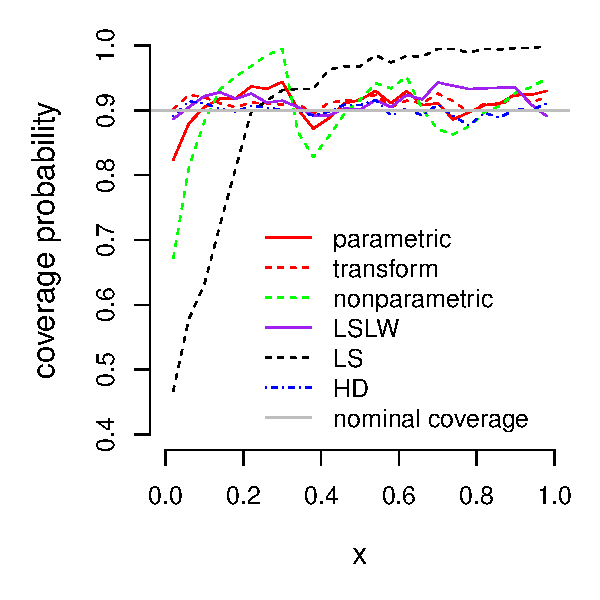
\includegraphics[width=\maxwidth]{figure/readme-inx-1} 

\end{knitrout}
\end{center}
\caption{Plot of the estimated coverage probabilities of prediction regions 
  across $x$.}
\label{Fig:coverageinx500.3}
\end{figure}




\newpage
\section{Additional Gamma simulations}
\label{sec:Gamma}

For the simulations in this section we generate responses using a gamma 
regression model with one variable.  We specify the inverse link function 
(the defualt in the \texttt{glm} function) and we set 
$\beta = (1.25, -1)^T$.  This value of $\beta$ is chosen so that the generated 
Gamma data is increasing, on average, in $x$ and exhibits increasing 
variability in $x$.  We investigate the performance of the five prediction 
regions across different sample size and shape parameter combinations.  We 
consider sample sizes of $n \in \{150, 250, 500\}$ and shape parameter values 
of $\{0.5, 0.75, 1, 1.5, 2, 5, 7, 10, 12, 15, 20, 25, 30, 40, 50, 60, 70, 80, 90, 100\}$.  
The LS and LSLW conformal prediction regions are fit using a cubic regression 
model.  This model is simple and it fits this type of Gamma data better than a 
simple linear or quadratic regression model.  Note that as the shape parameter 
increases the cubic regression model fits the data better.  When $n = 150$ we 
build the parametric and nonparametric conformal prediction regions using 2 
bins.  When $n = 250, 500$ we build the parametric and nonparametric conformal 
prediction regions using 3 bins.  These number of bin choices correspond to 
the bin width asymptotics of \citet{lei2014distribution}.

The next subsection contains all the code necessary to reproduce our results 
in Section~\ref{sec:Gamma-Results}.



\subsection{Simulations}

The following performs our Monte Carlo simulation of $B = 250$ iterations 
when $n = 150$ and shape = $0.5$.

\begin{knitrout}
\definecolor{shadecolor}{rgb}{0.969, 0.969, 0.969}\color{fgcolor}\begin{kframe}
\begin{alltt}
\hlkwd{set.seed}\hlstd{(}\hlnum{13}\hlstd{)}
\hlstd{beta} \hlkwb{<-} \hlkwd{c}\hlstd{(}\hlnum{1.25}\hlstd{,} \hlopt{-}\hlnum{1}\hlstd{)}
\hlstd{bins} \hlkwb{<-} \hlnum{2}
\hlstd{n} \hlkwb{<-} \hlnum{150}
\hlstd{B} \hlkwb{<-} \hlnum{250}
\hlkwd{system.time}\hlstd{(out.gamma.150.2.0.5} \hlkwb{<-} \hlkwd{do.call}\hlstd{(cbind,}
  \hlkwd{lapply}\hlstd{(}\hlnum{1}\hlopt{:}\hlstd{B,} \hlkwc{FUN} \hlstd{=} \hlkwa{function}\hlstd{(}\hlkwc{j}\hlstd{)\{}
    \hlkwd{unlist}\hlstd{(}\hlkwd{gamma.simulator}\hlstd{(}\hlkwc{beta} \hlstd{= beta,} \hlkwc{n} \hlstd{= n,}
      \hlkwc{bins} \hlstd{= bins,} \hlkwc{shape} \hlstd{=} \hlnum{0.5}\hlstd{))}
\hlstd{\})))}
\end{alltt}
\begin{verbatim}
##     user   system  elapsed 
## 7473.082   70.418 4733.124
\end{verbatim}
\end{kframe}
\end{knitrout}

\begin{knitrout}
\definecolor{shadecolor}{rgb}{0.969, 0.969, 0.969}\color{fgcolor}\begin{kframe}
\begin{alltt}
\hlstd{gamma.150.2.0.5} \hlkwb{<-} \hlkwd{cbind}\hlstd{(}
  \hlkwd{rowMeans}\hlstd{(out.gamma.150.2.0.5,} \hlkwc{na.rm} \hlstd{=} \hlnum{TRUE}\hlstd{),}
  \hlkwd{apply}\hlstd{(out.gamma.150.2.0.5,} \hlnum{1}\hlstd{,}
  \hlkwc{FUN} \hlstd{=} \hlkwa{function}\hlstd{(}\hlkwc{x}\hlstd{)\{}
    \hlstd{sds} \hlkwb{<-} \hlkwd{sd}\hlstd{(x,} \hlkwc{na.rm} \hlstd{=} \hlnum{TRUE}\hlstd{)}
    \hlstd{lengths} \hlkwb{<-} \hlkwd{length}\hlstd{(}\hlkwd{which}\hlstd{(}\hlopt{!}\hlkwd{is.na}\hlstd{(x)))}
    \hlstd{sds} \hlopt{/} \hlkwd{sqrt}\hlstd{(lengths)}
  \hlstd{\}))}
\end{alltt}
\end{kframe}
\end{knitrout}

The following performs our Monte Carlo simulation of $B = 250$ iterations 
when $n = 150$ and shape = $0.75$.

\begin{knitrout}
\definecolor{shadecolor}{rgb}{0.969, 0.969, 0.969}\color{fgcolor}\begin{kframe}
\begin{alltt}
\hlkwd{system.time}\hlstd{(out.gamma.150.2.0.75} \hlkwb{<-} \hlkwd{do.call}\hlstd{(cbind,}
  \hlkwd{lapply}\hlstd{(}\hlnum{1}\hlopt{:}\hlstd{B,} \hlkwc{FUN} \hlstd{=} \hlkwa{function}\hlstd{(}\hlkwc{j}\hlstd{)\{}
    \hlkwd{unlist}\hlstd{(}\hlkwd{gamma.simulator}\hlstd{(}\hlkwc{beta} \hlstd{= beta,} \hlkwc{n} \hlstd{= n,}
      \hlkwc{bins} \hlstd{= bins,} \hlkwc{shape} \hlstd{=} \hlnum{0.75}\hlstd{))}
\hlstd{\})))}
\end{alltt}
\begin{verbatim}
##     user   system  elapsed 
## 7308.074   67.704 4385.919
\end{verbatim}
\end{kframe}
\end{knitrout}

\begin{knitrout}
\definecolor{shadecolor}{rgb}{0.969, 0.969, 0.969}\color{fgcolor}\begin{kframe}
\begin{alltt}
\hlstd{gamma.150.2.0.75} \hlkwb{<-} \hlkwd{cbind}\hlstd{(}
  \hlkwd{rowMeans}\hlstd{(out.gamma.150.2.0.75,} \hlkwc{na.rm} \hlstd{=} \hlnum{TRUE}\hlstd{),}
  \hlkwd{apply}\hlstd{(out.gamma.150.2.0.75,} \hlnum{1}\hlstd{,}
  \hlkwc{FUN} \hlstd{=} \hlkwa{function}\hlstd{(}\hlkwc{x}\hlstd{)\{}
    \hlstd{sds} \hlkwb{<-} \hlkwd{sd}\hlstd{(x,} \hlkwc{na.rm} \hlstd{=} \hlnum{TRUE}\hlstd{)}
    \hlstd{lengths} \hlkwb{<-} \hlkwd{length}\hlstd{(}\hlkwd{which}\hlstd{(}\hlopt{!}\hlkwd{is.na}\hlstd{(x)))}
    \hlstd{sds} \hlopt{/} \hlkwd{sqrt}\hlstd{(lengths)}
  \hlstd{\}))}
\end{alltt}
\end{kframe}
\end{knitrout}

The following performs our Monte Carlo simulation of $B = 250$ iterations 
when $n = 150$ and shape = $1$.

\begin{knitrout}
\definecolor{shadecolor}{rgb}{0.969, 0.969, 0.969}\color{fgcolor}\begin{kframe}
\begin{alltt}
\hlkwd{system.time}\hlstd{(out.gamma.150.2.1} \hlkwb{<-} \hlkwd{do.call}\hlstd{(cbind,}
  \hlkwd{lapply}\hlstd{(}\hlnum{1}\hlopt{:}\hlstd{B,} \hlkwc{FUN} \hlstd{=} \hlkwa{function}\hlstd{(}\hlkwc{j}\hlstd{)\{}
    \hlkwd{unlist}\hlstd{(}\hlkwd{gamma.simulator}\hlstd{(}\hlkwc{beta} \hlstd{= beta,} \hlkwc{n} \hlstd{= n,}
      \hlkwc{bins} \hlstd{= bins,} \hlkwc{shape} \hlstd{=} \hlnum{1}\hlstd{))}
\hlstd{\})))}
\end{alltt}
\begin{verbatim}
##     user   system  elapsed 
## 6992.204   67.186 4018.650
\end{verbatim}
\end{kframe}
\end{knitrout}

\begin{knitrout}
\definecolor{shadecolor}{rgb}{0.969, 0.969, 0.969}\color{fgcolor}\begin{kframe}
\begin{alltt}
\hlstd{gamma.150.2.1} \hlkwb{<-} \hlkwd{cbind}\hlstd{(}
  \hlkwd{rowMeans}\hlstd{(out.gamma.150.2.1,} \hlkwc{na.rm} \hlstd{=} \hlnum{TRUE}\hlstd{),}
  \hlkwd{apply}\hlstd{(out.gamma.150.2.1,} \hlnum{1}\hlstd{,}
  \hlkwc{FUN} \hlstd{=} \hlkwa{function}\hlstd{(}\hlkwc{x}\hlstd{)\{}
    \hlstd{sds} \hlkwb{<-} \hlkwd{sd}\hlstd{(x,} \hlkwc{na.rm} \hlstd{=} \hlnum{TRUE}\hlstd{)}
    \hlstd{lengths} \hlkwb{<-} \hlkwd{length}\hlstd{(}\hlkwd{which}\hlstd{(}\hlopt{!}\hlkwd{is.na}\hlstd{(x)))}
    \hlstd{sds} \hlopt{/} \hlkwd{sqrt}\hlstd{(lengths)}
  \hlstd{\}))}
\end{alltt}
\end{kframe}
\end{knitrout}

The following performs our Monte Carlo simulation of $B = 250$ iterations 
when $n = 150$ and shape = $1.5$.

\begin{knitrout}
\definecolor{shadecolor}{rgb}{0.969, 0.969, 0.969}\color{fgcolor}\begin{kframe}
\begin{alltt}
\hlkwd{system.time}\hlstd{(out.gamma.150.2.1.5} \hlkwb{<-} \hlkwd{do.call}\hlstd{(cbind,}
  \hlkwd{lapply}\hlstd{(}\hlnum{1}\hlopt{:}\hlstd{B,} \hlkwc{FUN} \hlstd{=} \hlkwa{function}\hlstd{(}\hlkwc{j}\hlstd{)\{}
    \hlkwd{unlist}\hlstd{(}\hlkwd{gamma.simulator}\hlstd{(}\hlkwc{beta} \hlstd{= beta,} \hlkwc{n} \hlstd{= n,}
      \hlkwc{bins} \hlstd{= bins,} \hlkwc{shape} \hlstd{=} \hlnum{1.5}\hlstd{))}
\hlstd{\})))}
\end{alltt}
\begin{verbatim}
##      user    system   elapsed 
##  7456.522    67.902 10638.787
\end{verbatim}
\end{kframe}
\end{knitrout}

\begin{knitrout}
\definecolor{shadecolor}{rgb}{0.969, 0.969, 0.969}\color{fgcolor}\begin{kframe}
\begin{alltt}
\hlstd{gamma.150.2.1.5} \hlkwb{<-} \hlkwd{cbind}\hlstd{(}
  \hlkwd{rowMeans}\hlstd{(out.gamma.150.2.1.5,} \hlkwc{na.rm} \hlstd{=} \hlnum{TRUE}\hlstd{),}
  \hlkwd{apply}\hlstd{(out.gamma.150.2.1.5,} \hlnum{1}\hlstd{,}
  \hlkwc{FUN} \hlstd{=} \hlkwa{function}\hlstd{(}\hlkwc{x}\hlstd{)\{}
    \hlstd{sds} \hlkwb{<-} \hlkwd{sd}\hlstd{(x,} \hlkwc{na.rm} \hlstd{=} \hlnum{TRUE}\hlstd{)}
    \hlstd{lengths} \hlkwb{<-} \hlkwd{length}\hlstd{(}\hlkwd{which}\hlstd{(}\hlopt{!}\hlkwd{is.na}\hlstd{(x)))}
    \hlstd{sds} \hlopt{/} \hlkwd{sqrt}\hlstd{(lengths)}
  \hlstd{\}))}
\end{alltt}
\end{kframe}
\end{knitrout}

The following performs our Monte Carlo simulation of $B = 250$ iterations 
when $n = 150$ and shape = $2$.

\begin{knitrout}
\definecolor{shadecolor}{rgb}{0.969, 0.969, 0.969}\color{fgcolor}\begin{kframe}
\begin{alltt}
\hlkwd{system.time}\hlstd{(out.gamma.150.2.2} \hlkwb{<-} \hlkwd{do.call}\hlstd{(cbind,}
  \hlkwd{lapply}\hlstd{(}\hlnum{1}\hlopt{:}\hlstd{B,} \hlkwc{FUN} \hlstd{=} \hlkwa{function}\hlstd{(}\hlkwc{j}\hlstd{)\{}
    \hlkwd{unlist}\hlstd{(}\hlkwd{gamma.simulator}\hlstd{(}\hlkwc{beta} \hlstd{= beta,} \hlkwc{n} \hlstd{= n,}
      \hlkwc{bins} \hlstd{= bins,} \hlkwc{shape} \hlstd{=} \hlnum{2}\hlstd{))}
\hlstd{\})))}
\end{alltt}
\begin{verbatim}
##     user   system  elapsed 
## 8411.829   71.428 4583.947
\end{verbatim}
\end{kframe}
\end{knitrout}

\begin{knitrout}
\definecolor{shadecolor}{rgb}{0.969, 0.969, 0.969}\color{fgcolor}\begin{kframe}
\begin{alltt}
\hlstd{gamma.150.2.2} \hlkwb{<-} \hlkwd{cbind}\hlstd{(}
  \hlkwd{rowMeans}\hlstd{(out.gamma.150.2.2,} \hlkwc{na.rm} \hlstd{=} \hlnum{TRUE}\hlstd{),}
  \hlkwd{apply}\hlstd{(out.gamma.150.2.2,} \hlnum{1}\hlstd{,}
  \hlkwc{FUN} \hlstd{=} \hlkwa{function}\hlstd{(}\hlkwc{x}\hlstd{)\{}
    \hlstd{sds} \hlkwb{<-} \hlkwd{sd}\hlstd{(x,} \hlkwc{na.rm} \hlstd{=} \hlnum{TRUE}\hlstd{)}
    \hlstd{lengths} \hlkwb{<-} \hlkwd{length}\hlstd{(}\hlkwd{which}\hlstd{(}\hlopt{!}\hlkwd{is.na}\hlstd{(x)))}
    \hlstd{sds} \hlopt{/} \hlkwd{sqrt}\hlstd{(lengths)}
  \hlstd{\}))}
\end{alltt}
\end{kframe}
\end{knitrout}

The following performs our Monte Carlo simulation of $B = 250$ iterations 
when $n = 150$ and shape = $5$.

\begin{knitrout}
\definecolor{shadecolor}{rgb}{0.969, 0.969, 0.969}\color{fgcolor}\begin{kframe}
\begin{alltt}
\hlkwd{system.time}\hlstd{(out.gamma.150.2.5} \hlkwb{<-} \hlkwd{do.call}\hlstd{(cbind,}
  \hlkwd{lapply}\hlstd{(}\hlnum{1}\hlopt{:}\hlstd{B,} \hlkwc{FUN} \hlstd{=} \hlkwa{function}\hlstd{(}\hlkwc{j}\hlstd{)\{}
    \hlkwd{unlist}\hlstd{(}\hlkwd{gamma.simulator}\hlstd{(}\hlkwc{beta} \hlstd{= beta,} \hlkwc{n} \hlstd{= n,}
      \hlkwc{bins} \hlstd{= bins,} \hlkwc{shape} \hlstd{=} \hlnum{5}\hlstd{))}
\hlstd{\})))}
\end{alltt}
\begin{verbatim}
##     user   system  elapsed 
## 7584.710   64.449 4059.795
\end{verbatim}
\end{kframe}
\end{knitrout}

\begin{knitrout}
\definecolor{shadecolor}{rgb}{0.969, 0.969, 0.969}\color{fgcolor}\begin{kframe}
\begin{alltt}
\hlstd{gamma.150.2.5} \hlkwb{<-} \hlkwd{cbind}\hlstd{(}
  \hlkwd{rowMeans}\hlstd{(out.gamma.150.2.5,} \hlkwc{na.rm} \hlstd{=} \hlnum{TRUE}\hlstd{),}
  \hlkwd{apply}\hlstd{(out.gamma.150.2.5,} \hlnum{1}\hlstd{,}
  \hlkwc{FUN} \hlstd{=} \hlkwa{function}\hlstd{(}\hlkwc{x}\hlstd{)\{}
    \hlstd{sds} \hlkwb{<-} \hlkwd{sd}\hlstd{(x,} \hlkwc{na.rm} \hlstd{=} \hlnum{TRUE}\hlstd{)}
    \hlstd{lengths} \hlkwb{<-} \hlkwd{length}\hlstd{(}\hlkwd{which}\hlstd{(}\hlopt{!}\hlkwd{is.na}\hlstd{(x)))}
    \hlstd{sds} \hlopt{/} \hlkwd{sqrt}\hlstd{(lengths)}
  \hlstd{\}))}
\end{alltt}
\end{kframe}
\end{knitrout}

The following performs our Monte Carlo simulation of $B = 250$ iterations 
when $n = 150$ and shape = $7$.

\begin{knitrout}
\definecolor{shadecolor}{rgb}{0.969, 0.969, 0.969}\color{fgcolor}\begin{kframe}
\begin{alltt}
\hlkwd{system.time}\hlstd{(out.gamma.150.2.7} \hlkwb{<-} \hlkwd{do.call}\hlstd{(cbind,}
  \hlkwd{lapply}\hlstd{(}\hlnum{1}\hlopt{:}\hlstd{B,} \hlkwc{FUN} \hlstd{=} \hlkwa{function}\hlstd{(}\hlkwc{j}\hlstd{)\{}
    \hlkwd{unlist}\hlstd{(}\hlkwd{gamma.simulator}\hlstd{(}\hlkwc{beta} \hlstd{= beta,} \hlkwc{n} \hlstd{= n,}
      \hlkwc{bins} \hlstd{= bins,} \hlkwc{shape} \hlstd{=} \hlnum{7}\hlstd{))}
\hlstd{\})))}
\end{alltt}
\begin{verbatim}
##     user   system  elapsed 
## 7562.858   65.481 4018.408
\end{verbatim}
\end{kframe}
\end{knitrout}

\begin{knitrout}
\definecolor{shadecolor}{rgb}{0.969, 0.969, 0.969}\color{fgcolor}\begin{kframe}
\begin{alltt}
\hlstd{gamma.150.2.7} \hlkwb{<-} \hlkwd{cbind}\hlstd{(}
  \hlkwd{rowMeans}\hlstd{(out.gamma.150.2.7,} \hlkwc{na.rm} \hlstd{=} \hlnum{TRUE}\hlstd{),}
  \hlkwd{apply}\hlstd{(out.gamma.150.2.7,} \hlnum{1}\hlstd{,}
  \hlkwc{FUN} \hlstd{=} \hlkwa{function}\hlstd{(}\hlkwc{x}\hlstd{)\{}
    \hlstd{sds} \hlkwb{<-} \hlkwd{sd}\hlstd{(x,} \hlkwc{na.rm} \hlstd{=} \hlnum{TRUE}\hlstd{)}
    \hlstd{lengths} \hlkwb{<-} \hlkwd{length}\hlstd{(}\hlkwd{which}\hlstd{(}\hlopt{!}\hlkwd{is.na}\hlstd{(x)))}
    \hlstd{sds} \hlopt{/} \hlkwd{sqrt}\hlstd{(lengths)}
  \hlstd{\}))}
\end{alltt}
\end{kframe}
\end{knitrout}

The following performs our Monte Carlo simulation of $B = 250$ iterations 
when $n = 150$ and shape = $10$.

\begin{knitrout}
\definecolor{shadecolor}{rgb}{0.969, 0.969, 0.969}\color{fgcolor}\begin{kframe}
\begin{alltt}
\hlkwd{system.time}\hlstd{(out.gamma.150.2.10} \hlkwb{<-} \hlkwd{do.call}\hlstd{(cbind,}
  \hlkwd{lapply}\hlstd{(}\hlnum{1}\hlopt{:}\hlstd{B,} \hlkwc{FUN} \hlstd{=} \hlkwa{function}\hlstd{(}\hlkwc{j}\hlstd{)\{}
    \hlkwd{unlist}\hlstd{(}\hlkwd{gamma.simulator}\hlstd{(}\hlkwc{beta} \hlstd{= beta,} \hlkwc{n} \hlstd{= n,}
      \hlkwc{bins} \hlstd{= bins,} \hlkwc{shape} \hlstd{=} \hlnum{10}\hlstd{))}
\hlstd{\})))}
\end{alltt}
\begin{verbatim}
##     user   system  elapsed 
## 7645.495   66.652 4035.760
\end{verbatim}
\end{kframe}
\end{knitrout}

\begin{knitrout}
\definecolor{shadecolor}{rgb}{0.969, 0.969, 0.969}\color{fgcolor}\begin{kframe}
\begin{alltt}
\hlstd{gamma.150.2.10} \hlkwb{<-} \hlkwd{cbind}\hlstd{(}
  \hlkwd{rowMeans}\hlstd{(out.gamma.150.2.10,} \hlkwc{na.rm} \hlstd{=} \hlnum{TRUE}\hlstd{),}
  \hlkwd{apply}\hlstd{(out.gamma.150.2.10,} \hlnum{1}\hlstd{,}
  \hlkwc{FUN} \hlstd{=} \hlkwa{function}\hlstd{(}\hlkwc{x}\hlstd{)\{}
    \hlstd{sds} \hlkwb{<-} \hlkwd{sd}\hlstd{(x,} \hlkwc{na.rm} \hlstd{=} \hlnum{TRUE}\hlstd{)}
    \hlstd{lengths} \hlkwb{<-} \hlkwd{length}\hlstd{(}\hlkwd{which}\hlstd{(}\hlopt{!}\hlkwd{is.na}\hlstd{(x)))}
    \hlstd{sds} \hlopt{/} \hlkwd{sqrt}\hlstd{(lengths)}
  \hlstd{\}))}
\end{alltt}
\end{kframe}
\end{knitrout}

The following performs our Monte Carlo simulation of $B = 250$ iterations 
when $n = 150$ and shape = $12$.

\begin{knitrout}
\definecolor{shadecolor}{rgb}{0.969, 0.969, 0.969}\color{fgcolor}\begin{kframe}
\begin{alltt}
\hlkwd{system.time}\hlstd{(out.gamma.150.2.12} \hlkwb{<-} \hlkwd{do.call}\hlstd{(cbind,}
  \hlkwd{lapply}\hlstd{(}\hlnum{1}\hlopt{:}\hlstd{B,} \hlkwc{FUN} \hlstd{=} \hlkwa{function}\hlstd{(}\hlkwc{j}\hlstd{)\{}
    \hlkwd{unlist}\hlstd{(}\hlkwd{gamma.simulator}\hlstd{(}\hlkwc{beta} \hlstd{= beta,} \hlkwc{n} \hlstd{= n,}
      \hlkwc{bins} \hlstd{= bins,} \hlkwc{shape} \hlstd{=} \hlnum{12}\hlstd{))}
\hlstd{\})))}
\end{alltt}
\begin{verbatim}
##     user   system  elapsed 
## 7641.583   65.990 4035.577
\end{verbatim}
\end{kframe}
\end{knitrout}

\begin{knitrout}
\definecolor{shadecolor}{rgb}{0.969, 0.969, 0.969}\color{fgcolor}\begin{kframe}
\begin{alltt}
\hlstd{gamma.150.2.12} \hlkwb{<-} \hlkwd{cbind}\hlstd{(}
  \hlkwd{rowMeans}\hlstd{(out.gamma.150.2.12,} \hlkwc{na.rm} \hlstd{=} \hlnum{TRUE}\hlstd{),}
  \hlkwd{apply}\hlstd{(out.gamma.150.2.12,} \hlnum{1}\hlstd{,}
  \hlkwc{FUN} \hlstd{=} \hlkwa{function}\hlstd{(}\hlkwc{x}\hlstd{)\{}
    \hlstd{sds} \hlkwb{<-} \hlkwd{sd}\hlstd{(x,} \hlkwc{na.rm} \hlstd{=} \hlnum{TRUE}\hlstd{)}
    \hlstd{lengths} \hlkwb{<-} \hlkwd{length}\hlstd{(}\hlkwd{which}\hlstd{(}\hlopt{!}\hlkwd{is.na}\hlstd{(x)))}
    \hlstd{sds} \hlopt{/} \hlkwd{sqrt}\hlstd{(lengths)}
  \hlstd{\}))}
\end{alltt}
\end{kframe}
\end{knitrout}

The following performs our Monte Carlo simulation of $B = 250$ iterations 
when $n = 150$ and shape = $15$.

\begin{knitrout}
\definecolor{shadecolor}{rgb}{0.969, 0.969, 0.969}\color{fgcolor}\begin{kframe}
\begin{alltt}
\hlkwd{system.time}\hlstd{(out.gamma.150.2.15} \hlkwb{<-} \hlkwd{do.call}\hlstd{(cbind,}
  \hlkwd{lapply}\hlstd{(}\hlnum{1}\hlopt{:}\hlstd{B,} \hlkwc{FUN} \hlstd{=} \hlkwa{function}\hlstd{(}\hlkwc{j}\hlstd{)\{}
    \hlkwd{unlist}\hlstd{(}\hlkwd{gamma.simulator}\hlstd{(}\hlkwc{beta} \hlstd{= beta,} \hlkwc{n} \hlstd{= n,}
      \hlkwc{bins} \hlstd{= bins,} \hlkwc{shape} \hlstd{=} \hlnum{15}\hlstd{))}
\hlstd{\})))}
\end{alltt}
\begin{verbatim}
##     user   system  elapsed 
## 7535.949   65.387 4003.467
\end{verbatim}
\end{kframe}
\end{knitrout}

\begin{knitrout}
\definecolor{shadecolor}{rgb}{0.969, 0.969, 0.969}\color{fgcolor}\begin{kframe}
\begin{alltt}
\hlstd{gamma.150.2.15} \hlkwb{<-} \hlkwd{cbind}\hlstd{(}
  \hlkwd{rowMeans}\hlstd{(out.gamma.150.2.15,} \hlkwc{na.rm} \hlstd{=} \hlnum{TRUE}\hlstd{),}
  \hlkwd{apply}\hlstd{(out.gamma.150.2.15,} \hlnum{1}\hlstd{,}
  \hlkwc{FUN} \hlstd{=} \hlkwa{function}\hlstd{(}\hlkwc{x}\hlstd{)\{}
    \hlstd{sds} \hlkwb{<-} \hlkwd{sd}\hlstd{(x,} \hlkwc{na.rm} \hlstd{=} \hlnum{TRUE}\hlstd{)}
    \hlstd{lengths} \hlkwb{<-} \hlkwd{length}\hlstd{(}\hlkwd{which}\hlstd{(}\hlopt{!}\hlkwd{is.na}\hlstd{(x)))}
    \hlstd{sds} \hlopt{/} \hlkwd{sqrt}\hlstd{(lengths)}
  \hlstd{\}))}
\end{alltt}
\end{kframe}
\end{knitrout}

The following performs our Monte Carlo simulation of $B = 250$ iterations 
when $n = 150$ and shape = $20$.

\begin{knitrout}
\definecolor{shadecolor}{rgb}{0.969, 0.969, 0.969}\color{fgcolor}\begin{kframe}
\begin{alltt}
\hlkwd{system.time}\hlstd{(out.gamma.150.2.20} \hlkwb{<-} \hlkwd{do.call}\hlstd{(cbind,}
  \hlkwd{lapply}\hlstd{(}\hlnum{1}\hlopt{:}\hlstd{B,} \hlkwc{FUN} \hlstd{=} \hlkwa{function}\hlstd{(}\hlkwc{j}\hlstd{)\{}
    \hlkwd{unlist}\hlstd{(}\hlkwd{gamma.simulator}\hlstd{(}\hlkwc{beta} \hlstd{= beta,} \hlkwc{n} \hlstd{= n,}
      \hlkwc{bins} \hlstd{= bins,} \hlkwc{shape} \hlstd{=} \hlnum{20}\hlstd{))}
\hlstd{\})))}
\end{alltt}
\begin{verbatim}
##     user   system  elapsed 
## 7850.360   66.055 4065.622
\end{verbatim}
\end{kframe}
\end{knitrout}

\begin{knitrout}
\definecolor{shadecolor}{rgb}{0.969, 0.969, 0.969}\color{fgcolor}\begin{kframe}
\begin{alltt}
\hlstd{gamma.150.2.20} \hlkwb{<-} \hlkwd{cbind}\hlstd{(}
  \hlkwd{rowMeans}\hlstd{(out.gamma.150.2.20,} \hlkwc{na.rm} \hlstd{=} \hlnum{TRUE}\hlstd{),}
  \hlkwd{apply}\hlstd{(out.gamma.150.2.20,} \hlnum{1}\hlstd{,}
  \hlkwc{FUN} \hlstd{=} \hlkwa{function}\hlstd{(}\hlkwc{x}\hlstd{)\{}
    \hlstd{sds} \hlkwb{<-} \hlkwd{sd}\hlstd{(x,} \hlkwc{na.rm} \hlstd{=} \hlnum{TRUE}\hlstd{)}
    \hlstd{lengths} \hlkwb{<-} \hlkwd{length}\hlstd{(}\hlkwd{which}\hlstd{(}\hlopt{!}\hlkwd{is.na}\hlstd{(x)))}
    \hlstd{sds} \hlopt{/} \hlkwd{sqrt}\hlstd{(lengths)}
  \hlstd{\}))}
\end{alltt}
\end{kframe}
\end{knitrout}

The following performs our Monte Carlo simulation of $B = 250$ iterations 
when $n = 150$ and shape = $25$.

\begin{knitrout}
\definecolor{shadecolor}{rgb}{0.969, 0.969, 0.969}\color{fgcolor}\begin{kframe}
\begin{alltt}
\hlkwd{system.time}\hlstd{(out.gamma.150.2.25} \hlkwb{<-} \hlkwd{do.call}\hlstd{(cbind,}
  \hlkwd{lapply}\hlstd{(}\hlnum{1}\hlopt{:}\hlstd{B,} \hlkwc{FUN} \hlstd{=} \hlkwa{function}\hlstd{(}\hlkwc{j}\hlstd{)\{}
    \hlkwd{unlist}\hlstd{(}\hlkwd{gamma.simulator}\hlstd{(}\hlkwc{beta} \hlstd{= beta,} \hlkwc{n} \hlstd{= n,}
      \hlkwc{bins} \hlstd{= bins,} \hlkwc{shape} \hlstd{=} \hlnum{25}\hlstd{))}
\hlstd{\})))}
\end{alltt}
\begin{verbatim}
##     user   system  elapsed 
## 7805.004   66.341 4057.034
\end{verbatim}
\end{kframe}
\end{knitrout}

\begin{knitrout}
\definecolor{shadecolor}{rgb}{0.969, 0.969, 0.969}\color{fgcolor}\begin{kframe}
\begin{alltt}
\hlstd{gamma.150.2.25} \hlkwb{<-} \hlkwd{cbind}\hlstd{(}
  \hlkwd{rowMeans}\hlstd{(out.gamma.150.2.25,} \hlkwc{na.rm} \hlstd{=} \hlnum{TRUE}\hlstd{),}
  \hlkwd{apply}\hlstd{(out.gamma.150.2.25,} \hlnum{1}\hlstd{,}
  \hlkwc{FUN} \hlstd{=} \hlkwa{function}\hlstd{(}\hlkwc{x}\hlstd{)\{}
    \hlstd{sds} \hlkwb{<-} \hlkwd{sd}\hlstd{(x,} \hlkwc{na.rm} \hlstd{=} \hlnum{TRUE}\hlstd{)}
    \hlstd{lengths} \hlkwb{<-} \hlkwd{length}\hlstd{(}\hlkwd{which}\hlstd{(}\hlopt{!}\hlkwd{is.na}\hlstd{(x)))}
    \hlstd{sds} \hlopt{/} \hlkwd{sqrt}\hlstd{(lengths)}
  \hlstd{\}))}
\end{alltt}
\end{kframe}
\end{knitrout}

The following performs our Monte Carlo simulation of $B = 250$ iterations 
when $n = 150$ and shape = $30$.

\begin{knitrout}
\definecolor{shadecolor}{rgb}{0.969, 0.969, 0.969}\color{fgcolor}\begin{kframe}
\begin{alltt}
\hlkwd{system.time}\hlstd{(out.gamma.150.2.30} \hlkwb{<-} \hlkwd{do.call}\hlstd{(cbind,}
  \hlkwd{lapply}\hlstd{(}\hlnum{1}\hlopt{:}\hlstd{B,} \hlkwc{FUN} \hlstd{=} \hlkwa{function}\hlstd{(}\hlkwc{j}\hlstd{)\{}
    \hlkwd{unlist}\hlstd{(}\hlkwd{gamma.simulator}\hlstd{(}\hlkwc{beta} \hlstd{= beta,} \hlkwc{n} \hlstd{= n,}
      \hlkwc{bins} \hlstd{= bins,} \hlkwc{shape} \hlstd{=} \hlnum{30}\hlstd{))}
\hlstd{\})))}
\end{alltt}
\begin{verbatim}
##     user   system  elapsed 
## 8044.189   68.723 4100.474
\end{verbatim}
\end{kframe}
\end{knitrout}

\begin{knitrout}
\definecolor{shadecolor}{rgb}{0.969, 0.969, 0.969}\color{fgcolor}\begin{kframe}
\begin{alltt}
\hlstd{gamma.150.2.30} \hlkwb{<-} \hlkwd{cbind}\hlstd{(}
  \hlkwd{rowMeans}\hlstd{(out.gamma.150.2.30,} \hlkwc{na.rm} \hlstd{=} \hlnum{TRUE}\hlstd{),}
  \hlkwd{apply}\hlstd{(out.gamma.150.2.30,} \hlnum{1}\hlstd{,}
  \hlkwc{FUN} \hlstd{=} \hlkwa{function}\hlstd{(}\hlkwc{x}\hlstd{)\{}
    \hlstd{sds} \hlkwb{<-} \hlkwd{sd}\hlstd{(x,} \hlkwc{na.rm} \hlstd{=} \hlnum{TRUE}\hlstd{)}
    \hlstd{lengths} \hlkwb{<-} \hlkwd{length}\hlstd{(}\hlkwd{which}\hlstd{(}\hlopt{!}\hlkwd{is.na}\hlstd{(x)))}
    \hlstd{sds} \hlopt{/} \hlkwd{sqrt}\hlstd{(lengths)}
  \hlstd{\}))}
\end{alltt}
\end{kframe}
\end{knitrout}

The following performs our Monte Carlo simulation of $B = 250$ iterations 
when $n = 150$ and shape = $40$.

\begin{knitrout}
\definecolor{shadecolor}{rgb}{0.969, 0.969, 0.969}\color{fgcolor}\begin{kframe}
\begin{alltt}
\hlkwd{system.time}\hlstd{(out.gamma.150.2.40} \hlkwb{<-} \hlkwd{do.call}\hlstd{(cbind,}
  \hlkwd{lapply}\hlstd{(}\hlnum{1}\hlopt{:}\hlstd{B,} \hlkwc{FUN} \hlstd{=} \hlkwa{function}\hlstd{(}\hlkwc{j}\hlstd{)\{}
    \hlkwd{unlist}\hlstd{(}\hlkwd{gamma.simulator}\hlstd{(}\hlkwc{beta} \hlstd{= beta,} \hlkwc{n} \hlstd{= n,}
      \hlkwc{bins} \hlstd{= bins,} \hlkwc{shape} \hlstd{=} \hlnum{40}\hlstd{))}
\hlstd{\})))}
\end{alltt}
\begin{verbatim}
##     user   system  elapsed 
## 7968.318   65.667 4073.458
\end{verbatim}
\end{kframe}
\end{knitrout}

\begin{knitrout}
\definecolor{shadecolor}{rgb}{0.969, 0.969, 0.969}\color{fgcolor}\begin{kframe}
\begin{alltt}
\hlstd{gamma.150.2.40} \hlkwb{<-} \hlkwd{cbind}\hlstd{(}
  \hlkwd{rowMeans}\hlstd{(out.gamma.150.2.40,} \hlkwc{na.rm} \hlstd{=} \hlnum{TRUE}\hlstd{),}
  \hlkwd{apply}\hlstd{(out.gamma.150.2.40,} \hlnum{1}\hlstd{,}
  \hlkwc{FUN} \hlstd{=} \hlkwa{function}\hlstd{(}\hlkwc{x}\hlstd{)\{}
    \hlstd{sds} \hlkwb{<-} \hlkwd{sd}\hlstd{(x,} \hlkwc{na.rm} \hlstd{=} \hlnum{TRUE}\hlstd{)}
    \hlstd{lengths} \hlkwb{<-} \hlkwd{length}\hlstd{(}\hlkwd{which}\hlstd{(}\hlopt{!}\hlkwd{is.na}\hlstd{(x)))}
    \hlstd{sds} \hlopt{/} \hlkwd{sqrt}\hlstd{(lengths)}
  \hlstd{\}))}
\end{alltt}
\end{kframe}
\end{knitrout}

The following performs our Monte Carlo simulation of $B = 250$ iterations 
when $n = 150$ and shape = $50$.

\begin{knitrout}
\definecolor{shadecolor}{rgb}{0.969, 0.969, 0.969}\color{fgcolor}\begin{kframe}
\begin{alltt}
\hlkwd{system.time}\hlstd{(out.gamma.150.2.50} \hlkwb{<-} \hlkwd{do.call}\hlstd{(cbind,}
  \hlkwd{lapply}\hlstd{(}\hlnum{1}\hlopt{:}\hlstd{B,} \hlkwc{FUN} \hlstd{=} \hlkwa{function}\hlstd{(}\hlkwc{j}\hlstd{)\{}
    \hlkwd{unlist}\hlstd{(}\hlkwd{gamma.simulator}\hlstd{(}\hlkwc{beta} \hlstd{= beta,} \hlkwc{n} \hlstd{= n,}
      \hlkwc{bins} \hlstd{= bins,} \hlkwc{shape} \hlstd{=} \hlnum{50}\hlstd{))}
\hlstd{\})))}
\end{alltt}
\begin{verbatim}
##     user   system  elapsed 
## 8087.560   66.821 4086.898
\end{verbatim}
\end{kframe}
\end{knitrout}

\begin{knitrout}
\definecolor{shadecolor}{rgb}{0.969, 0.969, 0.969}\color{fgcolor}\begin{kframe}
\begin{alltt}
\hlstd{gamma.150.2.50} \hlkwb{<-} \hlkwd{cbind}\hlstd{(}
  \hlkwd{rowMeans}\hlstd{(out.gamma.150.2.50,} \hlkwc{na.rm} \hlstd{=} \hlnum{TRUE}\hlstd{),}
  \hlkwd{apply}\hlstd{(out.gamma.150.2.50,} \hlnum{1}\hlstd{,}
  \hlkwc{FUN} \hlstd{=} \hlkwa{function}\hlstd{(}\hlkwc{x}\hlstd{)\{}
    \hlstd{sds} \hlkwb{<-} \hlkwd{sd}\hlstd{(x,} \hlkwc{na.rm} \hlstd{=} \hlnum{TRUE}\hlstd{)}
    \hlstd{lengths} \hlkwb{<-} \hlkwd{length}\hlstd{(}\hlkwd{which}\hlstd{(}\hlopt{!}\hlkwd{is.na}\hlstd{(x)))}
    \hlstd{sds} \hlopt{/} \hlkwd{sqrt}\hlstd{(lengths)}
  \hlstd{\}))}
\end{alltt}
\end{kframe}
\end{knitrout}

The following performs our Monte Carlo simulation of $B = 250$ iterations 
when $n = 150$ and shape = $60$.

\begin{knitrout}
\definecolor{shadecolor}{rgb}{0.969, 0.969, 0.969}\color{fgcolor}\begin{kframe}
\begin{alltt}
\hlkwd{system.time}\hlstd{(out.gamma.150.2.60} \hlkwb{<-} \hlkwd{do.call}\hlstd{(cbind,}
  \hlkwd{lapply}\hlstd{(}\hlnum{1}\hlopt{:}\hlstd{B,} \hlkwc{FUN} \hlstd{=} \hlkwa{function}\hlstd{(}\hlkwc{j}\hlstd{)\{}
    \hlkwd{unlist}\hlstd{(}\hlkwd{gamma.simulator}\hlstd{(}\hlkwc{beta} \hlstd{= beta,} \hlkwc{n} \hlstd{= n,}
      \hlkwc{bins} \hlstd{= bins,} \hlkwc{shape} \hlstd{=} \hlnum{60}\hlstd{))}
\hlstd{\})))}
\end{alltt}
\begin{verbatim}
##     user   system  elapsed 
## 8543.967   70.317 4309.284
\end{verbatim}
\end{kframe}
\end{knitrout}

\begin{knitrout}
\definecolor{shadecolor}{rgb}{0.969, 0.969, 0.969}\color{fgcolor}\begin{kframe}
\begin{alltt}
\hlstd{gamma.150.2.60} \hlkwb{<-} \hlkwd{cbind}\hlstd{(}
  \hlkwd{rowMeans}\hlstd{(out.gamma.150.2.60,} \hlkwc{na.rm} \hlstd{=} \hlnum{TRUE}\hlstd{),}
  \hlkwd{apply}\hlstd{(out.gamma.150.2.60,} \hlnum{1}\hlstd{,}
  \hlkwc{FUN} \hlstd{=} \hlkwa{function}\hlstd{(}\hlkwc{x}\hlstd{)\{}
    \hlstd{sds} \hlkwb{<-} \hlkwd{sd}\hlstd{(x,} \hlkwc{na.rm} \hlstd{=} \hlnum{TRUE}\hlstd{)}
    \hlstd{lengths} \hlkwb{<-} \hlkwd{length}\hlstd{(}\hlkwd{which}\hlstd{(}\hlopt{!}\hlkwd{is.na}\hlstd{(x)))}
    \hlstd{sds} \hlopt{/} \hlkwd{sqrt}\hlstd{(lengths)}
  \hlstd{\}))}
\end{alltt}
\end{kframe}
\end{knitrout}

The following performs our Monte Carlo simulation of $B = 250$ iterations 
when $n = 150$ and shape = $70$.

\begin{knitrout}
\definecolor{shadecolor}{rgb}{0.969, 0.969, 0.969}\color{fgcolor}\begin{kframe}
\begin{alltt}
\hlkwd{system.time}\hlstd{(out.gamma.150.2.70} \hlkwb{<-} \hlkwd{do.call}\hlstd{(cbind,}
  \hlkwd{lapply}\hlstd{(}\hlnum{1}\hlopt{:}\hlstd{B,} \hlkwc{FUN} \hlstd{=} \hlkwa{function}\hlstd{(}\hlkwc{j}\hlstd{)\{}
    \hlkwd{unlist}\hlstd{(}\hlkwd{gamma.simulator}\hlstd{(}\hlkwc{beta} \hlstd{= beta,} \hlkwc{n} \hlstd{= n,}
      \hlkwc{bins} \hlstd{= bins,} \hlkwc{shape} \hlstd{=} \hlnum{70}\hlstd{))}
\hlstd{\})))}
\end{alltt}
\begin{verbatim}
##     user   system  elapsed 
## 9038.847   73.108 4394.150
\end{verbatim}
\end{kframe}
\end{knitrout}

\begin{knitrout}
\definecolor{shadecolor}{rgb}{0.969, 0.969, 0.969}\color{fgcolor}\begin{kframe}
\begin{alltt}
\hlstd{gamma.150.2.70} \hlkwb{<-} \hlkwd{cbind}\hlstd{(}
  \hlkwd{rowMeans}\hlstd{(out.gamma.150.2.70,} \hlkwc{na.rm} \hlstd{=} \hlnum{TRUE}\hlstd{),}
  \hlkwd{apply}\hlstd{(out.gamma.150.2.70,} \hlnum{1}\hlstd{,}
  \hlkwc{FUN} \hlstd{=} \hlkwa{function}\hlstd{(}\hlkwc{x}\hlstd{)\{}
    \hlstd{sds} \hlkwb{<-} \hlkwd{sd}\hlstd{(x,} \hlkwc{na.rm} \hlstd{=} \hlnum{TRUE}\hlstd{)}
    \hlstd{lengths} \hlkwb{<-} \hlkwd{length}\hlstd{(}\hlkwd{which}\hlstd{(}\hlopt{!}\hlkwd{is.na}\hlstd{(x)))}
    \hlstd{sds} \hlopt{/} \hlkwd{sqrt}\hlstd{(lengths)}
  \hlstd{\}))}
\end{alltt}
\end{kframe}
\end{knitrout}

The following performs our Monte Carlo simulation of $B = 250$ iterations 
when $n = 150$ and shape = $80$.

\begin{knitrout}
\definecolor{shadecolor}{rgb}{0.969, 0.969, 0.969}\color{fgcolor}\begin{kframe}
\begin{alltt}
\hlkwd{system.time}\hlstd{(out.gamma.150.2.80} \hlkwb{<-} \hlkwd{do.call}\hlstd{(cbind,}
  \hlkwd{lapply}\hlstd{(}\hlnum{1}\hlopt{:}\hlstd{B,} \hlkwc{FUN} \hlstd{=} \hlkwa{function}\hlstd{(}\hlkwc{j}\hlstd{)\{}
    \hlkwd{unlist}\hlstd{(}\hlkwd{gamma.simulator}\hlstd{(}\hlkwc{beta} \hlstd{= beta,} \hlkwc{n} \hlstd{= n,}
      \hlkwc{bins} \hlstd{= bins,} \hlkwc{shape} \hlstd{=} \hlnum{80}\hlstd{))}
\hlstd{\})))}
\end{alltt}
\begin{verbatim}
##     user   system  elapsed 
## 9580.813   75.711 4638.776
\end{verbatim}
\end{kframe}
\end{knitrout}

\begin{knitrout}
\definecolor{shadecolor}{rgb}{0.969, 0.969, 0.969}\color{fgcolor}\begin{kframe}
\begin{alltt}
\hlstd{gamma.150.2.80} \hlkwb{<-} \hlkwd{cbind}\hlstd{(}
  \hlkwd{rowMeans}\hlstd{(out.gamma.150.2.80,} \hlkwc{na.rm} \hlstd{=} \hlnum{TRUE}\hlstd{),}
  \hlkwd{apply}\hlstd{(out.gamma.150.2.80,} \hlnum{1}\hlstd{,}
  \hlkwc{FUN} \hlstd{=} \hlkwa{function}\hlstd{(}\hlkwc{x}\hlstd{)\{}
    \hlstd{sds} \hlkwb{<-} \hlkwd{sd}\hlstd{(x,} \hlkwc{na.rm} \hlstd{=} \hlnum{TRUE}\hlstd{)}
    \hlstd{lengths} \hlkwb{<-} \hlkwd{length}\hlstd{(}\hlkwd{which}\hlstd{(}\hlopt{!}\hlkwd{is.na}\hlstd{(x)))}
    \hlstd{sds} \hlopt{/} \hlkwd{sqrt}\hlstd{(lengths)}
  \hlstd{\}))}
\end{alltt}
\end{kframe}
\end{knitrout}

The following performs our Monte Carlo simulation of $B = 250$ iterations 
when $n = 150$ and shape = $90$.

\begin{knitrout}
\definecolor{shadecolor}{rgb}{0.969, 0.969, 0.969}\color{fgcolor}\begin{kframe}
\begin{alltt}
\hlkwd{system.time}\hlstd{(out.gamma.150.2.90} \hlkwb{<-} \hlkwd{do.call}\hlstd{(cbind,}
  \hlkwd{lapply}\hlstd{(}\hlnum{1}\hlopt{:}\hlstd{B,} \hlkwc{FUN} \hlstd{=} \hlkwa{function}\hlstd{(}\hlkwc{j}\hlstd{)\{}
    \hlkwd{unlist}\hlstd{(}\hlkwd{gamma.simulator}\hlstd{(}\hlkwc{beta} \hlstd{= beta,} \hlkwc{n} \hlstd{= n,}
      \hlkwc{bins} \hlstd{= bins,} \hlkwc{shape} \hlstd{=} \hlnum{90}\hlstd{))}
\hlstd{\})))}
\end{alltt}
\begin{verbatim}
##     user   system  elapsed 
## 9410.124   74.038 4608.842
\end{verbatim}
\end{kframe}
\end{knitrout}

\begin{knitrout}
\definecolor{shadecolor}{rgb}{0.969, 0.969, 0.969}\color{fgcolor}\begin{kframe}
\begin{alltt}
\hlstd{gamma.150.2.90} \hlkwb{<-} \hlkwd{cbind}\hlstd{(}
  \hlkwd{rowMeans}\hlstd{(out.gamma.150.2.90,} \hlkwc{na.rm} \hlstd{=} \hlnum{TRUE}\hlstd{),}
  \hlkwd{apply}\hlstd{(out.gamma.150.2.90,} \hlnum{1}\hlstd{,}
  \hlkwc{FUN} \hlstd{=} \hlkwa{function}\hlstd{(}\hlkwc{x}\hlstd{)\{}
    \hlstd{sds} \hlkwb{<-} \hlkwd{sd}\hlstd{(x,} \hlkwc{na.rm} \hlstd{=} \hlnum{TRUE}\hlstd{)}
    \hlstd{lengths} \hlkwb{<-} \hlkwd{length}\hlstd{(}\hlkwd{which}\hlstd{(}\hlopt{!}\hlkwd{is.na}\hlstd{(x)))}
    \hlstd{sds} \hlopt{/} \hlkwd{sqrt}\hlstd{(lengths)}
  \hlstd{\}))}
\end{alltt}
\end{kframe}
\end{knitrout}

The following performs our Monte Carlo simulation of $B = 250$ iterations 
when $n = 150$ and shape = $100$.

\begin{knitrout}
\definecolor{shadecolor}{rgb}{0.969, 0.969, 0.969}\color{fgcolor}\begin{kframe}
\begin{alltt}
\hlkwd{system.time}\hlstd{(out.gamma.150.2.100} \hlkwb{<-} \hlkwd{do.call}\hlstd{(cbind,}
  \hlkwd{lapply}\hlstd{(}\hlnum{1}\hlopt{:}\hlstd{B,} \hlkwc{FUN} \hlstd{=} \hlkwa{function}\hlstd{(}\hlkwc{j}\hlstd{)\{}
    \hlkwd{unlist}\hlstd{(}\hlkwd{gamma.simulator}\hlstd{(}\hlkwc{beta} \hlstd{= beta,} \hlkwc{n} \hlstd{= n,}
      \hlkwc{bins} \hlstd{= bins,} \hlkwc{shape} \hlstd{=} \hlnum{100}\hlstd{))}
\hlstd{\})))}
\end{alltt}
\begin{verbatim}
##     user   system  elapsed 
## 9667.834   76.044 4650.667
\end{verbatim}
\end{kframe}
\end{knitrout}

\begin{knitrout}
\definecolor{shadecolor}{rgb}{0.969, 0.969, 0.969}\color{fgcolor}\begin{kframe}
\begin{alltt}
\hlstd{gamma.150.2.100} \hlkwb{<-} \hlkwd{cbind}\hlstd{(}
  \hlkwd{rowMeans}\hlstd{(out.gamma.150.2.100,} \hlkwc{na.rm} \hlstd{=} \hlnum{TRUE}\hlstd{),}
  \hlkwd{apply}\hlstd{(out.gamma.150.2.100,} \hlnum{1}\hlstd{,}
  \hlkwc{FUN} \hlstd{=} \hlkwa{function}\hlstd{(}\hlkwc{x}\hlstd{)\{}
    \hlstd{sds} \hlkwb{<-} \hlkwd{sd}\hlstd{(x,} \hlkwc{na.rm} \hlstd{=} \hlnum{TRUE}\hlstd{)}
    \hlstd{lengths} \hlkwb{<-} \hlkwd{length}\hlstd{(}\hlkwd{which}\hlstd{(}\hlopt{!}\hlkwd{is.na}\hlstd{(x)))}
    \hlstd{sds} \hlopt{/} \hlkwd{sqrt}\hlstd{(lengths)}
  \hlstd{\}))}
\end{alltt}
\end{kframe}
\end{knitrout}


Reorganize the output.

\begin{knitrout}
\definecolor{shadecolor}{rgb}{0.969, 0.969, 0.969}\color{fgcolor}\begin{kframe}
\begin{alltt}
\hlstd{para.area.gamma.150} \hlkwb{<-} \hlstd{nonpara.area.gamma.150} \hlkwb{<-}
  \hlstd{LS.area.gamma.150} \hlkwb{<-} \hlstd{LSLW.area.gamma.150} \hlkwb{<-}
  \hlstd{HD.area.gamma.150} \hlkwb{<-} \hlkwa{NULL}
\hlstd{para.error.gamma.150} \hlkwb{<-} \hlstd{nonpara.error.gamma.150} \hlkwb{<-}
  \hlstd{LS.error.gamma.150} \hlkwb{<-} \hlstd{LSLW.error.gamma.150} \hlkwb{<-}
  \hlstd{HD.error.gamma.150} \hlkwb{<-} \hlkwa{NULL}
\hlstd{para.marginal.gamma.150} \hlkwb{<-} \hlstd{nonpara.marginal.gamma.150} \hlkwb{<-}
  \hlstd{LS.marginal.gamma.150} \hlkwb{<-} \hlstd{LSLW.marginal.gamma.150} \hlkwb{<-}
  \hlstd{HD.marginal.gamma.150} \hlkwb{<-} \hlkwa{NULL}
\hlstd{para.local.gamma.150} \hlkwb{<-} \hlstd{nonpara.local.gamma.150} \hlkwb{<-}
  \hlstd{LS.local.gamma.150} \hlkwb{<-} \hlstd{LSLW.local.gamma.150} \hlkwb{<-}
  \hlstd{HD.local.gamma.150} \hlkwb{<-} \hlkwa{NULL}
\hlstd{para.inx.gamma.150} \hlkwb{<-} \hlstd{nonpara.inx.gamma.150} \hlkwb{<-}
  \hlstd{LS.inx.gamma.150} \hlkwb{<-} \hlstd{LSLW.inx.gamma.150} \hlkwb{<-}
  \hlstd{HD.inx.gamma.150} \hlkwb{<-} \hlkwa{NULL}
\hlstd{shapes} \hlkwb{<-} \hlkwd{c}\hlstd{(}\hlnum{0.5}\hlstd{,} \hlnum{0.75}\hlstd{,} \hlnum{1}\hlstd{,} \hlnum{1.5}\hlstd{,} \hlnum{2}\hlstd{,} \hlnum{5}\hlstd{,} \hlnum{7}\hlstd{,} \hlnum{10}\hlstd{,} \hlnum{12}\hlstd{,} \hlnum{15}\hlstd{,} \hlnum{20}\hlstd{,} \hlnum{25}\hlstd{,}
  \hlnum{30}\hlstd{,} \hlnum{40}\hlstd{,} \hlnum{50}\hlstd{,} \hlnum{60}\hlstd{,} \hlnum{70}\hlstd{,} \hlnum{80}\hlstd{,} \hlnum{90}\hlstd{,} \hlnum{100}\hlstd{)}
\hlkwa{for}\hlstd{(j} \hlkwa{in} \hlstd{shapes )\{}
  \hlstd{internal.output} \hlkwb{<-}
    \hlkwd{eval}\hlstd{(}\hlkwd{parse}\hlstd{(}\hlkwc{text}\hlstd{=}\hlkwd{paste}\hlstd{(}\hlstr{"gamma.150.2"}\hlstd{, j,} \hlkwc{sep} \hlstd{=} \hlstr{"."}\hlstd{)))}
  \hlstd{k} \hlkwb{<-} \hlkwd{which}\hlstd{(shapes} \hlopt{==} \hlstd{j)}
  \hlstd{para.marginal.gamma.150[k]} \hlkwb{<-} \hlkwd{as.numeric}\hlstd{(internal.output[}\hlnum{1}\hlstd{,} \hlnum{1}\hlstd{])}
  \hlstd{para.local.gamma.150[}\hlkwd{c}\hlstd{((bins}\hlopt{*}\hlstd{(k}\hlopt{-}\hlnum{1}\hlstd{)}\hlopt{+}\hlnum{1}\hlstd{)}\hlopt{:}\hlstd{(bins}\hlopt{*}\hlstd{k))]} \hlkwb{<-}
    \hlkwd{as.numeric}\hlstd{(internal.output[}\hlnum{2}\hlopt{:}\hlnum{3}\hlstd{,} \hlnum{1}\hlstd{])}
  \hlstd{para.inx.gamma.150[}\hlkwd{c}\hlstd{((}\hlnum{25}\hlopt{*}\hlstd{(k}\hlopt{-}\hlnum{1}\hlstd{)}\hlopt{+}\hlnum{1}\hlstd{)}\hlopt{:}\hlstd{(}\hlnum{25}\hlopt{*}\hlstd{k))]} \hlkwb{<-}
    \hlkwd{as.numeric}\hlstd{(internal.output[}\hlnum{4}\hlopt{:}\hlnum{28}\hlstd{,} \hlnum{1}\hlstd{])}
  \hlstd{para.error.gamma.150[k]} \hlkwb{<-} \hlkwd{as.numeric}\hlstd{(internal.output[}\hlnum{29}\hlstd{,} \hlnum{1}\hlstd{])}
  \hlstd{para.area.gamma.150[k]} \hlkwb{<-} \hlkwd{as.numeric}\hlstd{(internal.output[}\hlnum{30}\hlstd{,} \hlnum{1}\hlstd{])}
  \hlstd{nonpara.marginal.gamma.150[k]} \hlkwb{<-} \hlkwd{as.numeric}\hlstd{(internal.output[}\hlnum{31}\hlstd{,} \hlnum{1}\hlstd{])}
  \hlstd{nonpara.local.gamma.150[}\hlkwd{c}\hlstd{((bins}\hlopt{*}\hlstd{(k}\hlopt{-}\hlnum{1}\hlstd{)}\hlopt{+}\hlnum{1}\hlstd{)}\hlopt{:}\hlstd{(bins}\hlopt{*}\hlstd{k))]} \hlkwb{<-}
    \hlkwd{as.numeric}\hlstd{(internal.output[}\hlnum{32}\hlopt{:}\hlnum{33}\hlstd{,} \hlnum{1}\hlstd{])}
  \hlstd{nonpara.inx.gamma.150[}\hlkwd{c}\hlstd{((}\hlnum{25}\hlopt{*}\hlstd{(k}\hlopt{-}\hlnum{1}\hlstd{)}\hlopt{+}\hlnum{1}\hlstd{)}\hlopt{:}\hlstd{(}\hlnum{25}\hlopt{*}\hlstd{k))]} \hlkwb{<-}
    \hlkwd{as.numeric}\hlstd{(internal.output[}\hlnum{34}\hlopt{:}\hlnum{58}\hlstd{,} \hlnum{1}\hlstd{])}
  \hlstd{nonpara.error.gamma.150[k]} \hlkwb{<-} \hlkwd{as.numeric}\hlstd{(internal.output[}\hlnum{59}\hlstd{,} \hlnum{1}\hlstd{])}
  \hlstd{nonpara.area.gamma.150[k]} \hlkwb{<-} \hlkwd{as.numeric}\hlstd{(internal.output[}\hlnum{60}\hlstd{,} \hlnum{1}\hlstd{])}
  \hlstd{LS.marginal.gamma.150[k]} \hlkwb{<-} \hlkwd{as.numeric}\hlstd{(internal.output[}\hlnum{61}\hlstd{,} \hlnum{1}\hlstd{])}
  \hlstd{LS.local.gamma.150[}\hlkwd{c}\hlstd{((bins}\hlopt{*}\hlstd{(k}\hlopt{-}\hlnum{1}\hlstd{)}\hlopt{+}\hlnum{1}\hlstd{)}\hlopt{:}\hlstd{(bins}\hlopt{*}\hlstd{k))]} \hlkwb{<-}
    \hlkwd{as.numeric}\hlstd{(internal.output[}\hlnum{62}\hlopt{:}\hlnum{63}\hlstd{,} \hlnum{1}\hlstd{])}
  \hlstd{LS.inx.gamma.150[}\hlkwd{c}\hlstd{((}\hlnum{25}\hlopt{*}\hlstd{(k}\hlopt{-}\hlnum{1}\hlstd{)}\hlopt{+}\hlnum{1}\hlstd{)}\hlopt{:}\hlstd{(}\hlnum{25}\hlopt{*}\hlstd{k))]} \hlkwb{<-}
    \hlkwd{as.numeric}\hlstd{(internal.output[}\hlnum{64}\hlopt{:}\hlnum{88}\hlstd{,} \hlnum{1}\hlstd{])}
  \hlstd{LS.error.gamma.150[k]} \hlkwb{<-} \hlkwd{as.numeric}\hlstd{(internal.output[}\hlnum{89}\hlstd{,} \hlnum{1}\hlstd{])}
  \hlstd{LS.area.gamma.150[k]} \hlkwb{<-} \hlkwd{as.numeric}\hlstd{(internal.output[}\hlnum{90}\hlstd{,} \hlnum{1}\hlstd{])}
  \hlstd{LSLW.marginal.gamma.150[k]} \hlkwb{<-} \hlkwd{as.numeric}\hlstd{(internal.output[}\hlnum{91}\hlstd{,} \hlnum{1}\hlstd{])}
  \hlstd{LSLW.local.gamma.150[}\hlkwd{c}\hlstd{((bins}\hlopt{*}\hlstd{(k}\hlopt{-}\hlnum{1}\hlstd{)}\hlopt{+}\hlnum{1}\hlstd{)}\hlopt{:}\hlstd{(bins}\hlopt{*}\hlstd{k))]} \hlkwb{<-}
    \hlkwd{as.numeric}\hlstd{(internal.output[}\hlnum{92}\hlopt{:}\hlnum{93}\hlstd{,} \hlnum{1}\hlstd{])}
  \hlstd{LSLW.inx.gamma.150[}\hlkwd{c}\hlstd{((}\hlnum{25}\hlopt{*}\hlstd{(k}\hlopt{-}\hlnum{1}\hlstd{)}\hlopt{+}\hlnum{1}\hlstd{)}\hlopt{:}\hlstd{(}\hlnum{25}\hlopt{*}\hlstd{k))]} \hlkwb{<-}
    \hlkwd{as.numeric}\hlstd{(internal.output[}\hlnum{94}\hlopt{:}\hlnum{118}\hlstd{,} \hlnum{1}\hlstd{])}
  \hlstd{LSLW.error.gamma.150[k]} \hlkwb{<-} \hlkwd{as.numeric}\hlstd{(internal.output[}\hlnum{119}\hlstd{,} \hlnum{1}\hlstd{])}
  \hlstd{LSLW.area.gamma.150[k]} \hlkwb{<-} \hlkwd{as.numeric}\hlstd{(internal.output[}\hlnum{120}\hlstd{,} \hlnum{1}\hlstd{])}
  \hlstd{HD.marginal.gamma.150[k]} \hlkwb{<-} \hlkwd{as.numeric}\hlstd{(internal.output[}\hlnum{121}\hlstd{,} \hlnum{1}\hlstd{])}
  \hlstd{HD.local.gamma.150[}\hlkwd{c}\hlstd{((bins}\hlopt{*}\hlstd{(k}\hlopt{-}\hlnum{1}\hlstd{)}\hlopt{+}\hlnum{1}\hlstd{)}\hlopt{:}\hlstd{(bins}\hlopt{*}\hlstd{k))]} \hlkwb{<-}
    \hlkwd{as.numeric}\hlstd{(internal.output[}\hlnum{122}\hlopt{:}\hlnum{123}\hlstd{,} \hlnum{1}\hlstd{])}
  \hlstd{HD.inx.gamma.150[}\hlkwd{c}\hlstd{((}\hlnum{25}\hlopt{*}\hlstd{(k}\hlopt{-}\hlnum{1}\hlstd{)}\hlopt{+}\hlnum{1}\hlstd{)}\hlopt{:}\hlstd{(}\hlnum{25}\hlopt{*}\hlstd{k))]} \hlkwb{<-}
    \hlkwd{as.numeric}\hlstd{(internal.output[}\hlnum{124}\hlopt{:}\hlnum{148}\hlstd{,} \hlnum{1}\hlstd{])}
  \hlstd{HD.error.gamma.150[k]} \hlkwb{<-} \hlkwd{as.numeric}\hlstd{(internal.output[}\hlnum{149}\hlstd{,} \hlnum{1}\hlstd{])}
  \hlstd{HD.area.gamma.150[k]} \hlkwb{<-} \hlkwd{as.numeric}\hlstd{(internal.output[}\hlnum{150}\hlstd{,} \hlnum{1}\hlstd{])}
\hlstd{\}}
\end{alltt}
\end{kframe}
\end{knitrout}


%% n = 250
The following performs our Monte Carlo simulation of $B = 50$ iterations 
when $n = 250$ and shape = $0.5$.

\begin{knitrout}
\definecolor{shadecolor}{rgb}{0.969, 0.969, 0.969}\color{fgcolor}\begin{kframe}
\begin{alltt}
\hlkwd{set.seed}\hlstd{(}\hlnum{13}\hlstd{)}
\hlstd{beta} \hlkwb{<-} \hlkwd{c}\hlstd{(}\hlnum{1.25}\hlstd{,} \hlopt{-}\hlnum{1}\hlstd{)}
\hlstd{bins} \hlkwb{<-} \hlnum{3}
\hlstd{n} \hlkwb{<-} \hlnum{250}
\hlstd{B} \hlkwb{<-} \hlnum{50}
\hlkwd{system.time}\hlstd{(out.gamma.250.3.0.5} \hlkwb{<-} \hlkwd{do.call}\hlstd{(cbind,}
  \hlkwd{lapply}\hlstd{(}\hlnum{1}\hlopt{:}\hlstd{B,} \hlkwc{FUN} \hlstd{=} \hlkwa{function}\hlstd{(}\hlkwc{j}\hlstd{)\{}
    \hlkwd{unlist}\hlstd{(}\hlkwd{gamma.simulator}\hlstd{(}\hlkwc{beta} \hlstd{= beta,} \hlkwc{n} \hlstd{= n,}
      \hlkwc{bins} \hlstd{= bins,} \hlkwc{shape} \hlstd{=} \hlnum{0.5}\hlstd{))}
\hlstd{\})))}
\end{alltt}
\begin{verbatim}
##     user   system  elapsed 
## 2511.339   16.860 1496.168
\end{verbatim}
\end{kframe}
\end{knitrout}

\begin{knitrout}
\definecolor{shadecolor}{rgb}{0.969, 0.969, 0.969}\color{fgcolor}\begin{kframe}
\begin{alltt}
\hlstd{gamma.250.3.0.5} \hlkwb{<-} \hlkwd{cbind}\hlstd{(}
  \hlkwd{rowMeans}\hlstd{(out.gamma.250.3.0.5,} \hlkwc{na.rm} \hlstd{=} \hlnum{TRUE}\hlstd{),}
  \hlkwd{apply}\hlstd{(out.gamma.250.3.0.5,} \hlnum{1}\hlstd{,}
  \hlkwc{FUN} \hlstd{=} \hlkwa{function}\hlstd{(}\hlkwc{x}\hlstd{)\{}
    \hlstd{sds} \hlkwb{<-} \hlkwd{sd}\hlstd{(x,} \hlkwc{na.rm} \hlstd{=} \hlnum{TRUE}\hlstd{)}
    \hlstd{lengths} \hlkwb{<-} \hlkwd{length}\hlstd{(}\hlkwd{which}\hlstd{(}\hlopt{!}\hlkwd{is.na}\hlstd{(x)))}
    \hlstd{sds} \hlopt{/} \hlkwd{sqrt}\hlstd{(lengths)}
  \hlstd{\}))}
\end{alltt}
\end{kframe}
\end{knitrout}

The following performs our Monte Carlo simulation of $B = 50$ iterations 
when $n = 250$ and shape = $0.75$.

\begin{knitrout}
\definecolor{shadecolor}{rgb}{0.969, 0.969, 0.969}\color{fgcolor}\begin{kframe}
\begin{alltt}
\hlkwd{system.time}\hlstd{(out.gamma.250.3.0.75} \hlkwb{<-} \hlkwd{do.call}\hlstd{(cbind,}
  \hlkwd{lapply}\hlstd{(}\hlnum{1}\hlopt{:}\hlstd{B,} \hlkwc{FUN} \hlstd{=} \hlkwa{function}\hlstd{(}\hlkwc{j}\hlstd{)\{}
    \hlkwd{unlist}\hlstd{(}\hlkwd{gamma.simulator}\hlstd{(}\hlkwc{beta} \hlstd{= beta,} \hlkwc{n} \hlstd{= n,}
      \hlkwc{bins} \hlstd{= bins,} \hlkwc{shape} \hlstd{=} \hlnum{0.75}\hlstd{))}
\hlstd{\})))}
\end{alltt}
\begin{verbatim}
##     user   system  elapsed 
## 2577.735   16.795 1500.989
\end{verbatim}
\end{kframe}
\end{knitrout}

\begin{knitrout}
\definecolor{shadecolor}{rgb}{0.969, 0.969, 0.969}\color{fgcolor}\begin{kframe}
\begin{alltt}
\hlstd{gamma.250.3.0.75} \hlkwb{<-} \hlkwd{cbind}\hlstd{(}
  \hlkwd{rowMeans}\hlstd{(out.gamma.250.3.0.75,} \hlkwc{na.rm} \hlstd{=} \hlnum{TRUE}\hlstd{),}
  \hlkwd{apply}\hlstd{(out.gamma.250.3.0.75,} \hlnum{1}\hlstd{,}
  \hlkwc{FUN} \hlstd{=} \hlkwa{function}\hlstd{(}\hlkwc{x}\hlstd{)\{}
    \hlstd{sds} \hlkwb{<-} \hlkwd{sd}\hlstd{(x,} \hlkwc{na.rm} \hlstd{=} \hlnum{TRUE}\hlstd{)}
    \hlstd{lengths} \hlkwb{<-} \hlkwd{length}\hlstd{(}\hlkwd{which}\hlstd{(}\hlopt{!}\hlkwd{is.na}\hlstd{(x)))}
    \hlstd{sds} \hlopt{/} \hlkwd{sqrt}\hlstd{(lengths)}
  \hlstd{\}))}
\end{alltt}
\end{kframe}
\end{knitrout}

The following performs our Monte Carlo simulation of $B = 50$ iterations 
when $n = 250$ and shape = $1$.

\begin{knitrout}
\definecolor{shadecolor}{rgb}{0.969, 0.969, 0.969}\color{fgcolor}\begin{kframe}
\begin{alltt}
\hlkwd{system.time}\hlstd{(out.gamma.250.3.1} \hlkwb{<-} \hlkwd{do.call}\hlstd{(cbind,}
  \hlkwd{lapply}\hlstd{(}\hlnum{1}\hlopt{:}\hlstd{B,} \hlkwc{FUN} \hlstd{=} \hlkwa{function}\hlstd{(}\hlkwc{j}\hlstd{)\{}
    \hlkwd{unlist}\hlstd{(}\hlkwd{gamma.simulator}\hlstd{(}\hlkwc{beta} \hlstd{= beta,} \hlkwc{n} \hlstd{= n,}
      \hlkwc{bins} \hlstd{= bins,} \hlkwc{shape} \hlstd{=} \hlnum{1}\hlstd{))}
\hlstd{\})))}
\end{alltt}
\begin{verbatim}
##     user   system  elapsed 
## 2694.797   16.807 1523.346
\end{verbatim}
\end{kframe}
\end{knitrout}

\begin{knitrout}
\definecolor{shadecolor}{rgb}{0.969, 0.969, 0.969}\color{fgcolor}\begin{kframe}
\begin{alltt}
\hlstd{gamma.250.3.1} \hlkwb{<-} \hlkwd{cbind}\hlstd{(}
  \hlkwd{rowMeans}\hlstd{(out.gamma.250.3.1,} \hlkwc{na.rm} \hlstd{=} \hlnum{TRUE}\hlstd{),}
  \hlkwd{apply}\hlstd{(out.gamma.250.3.1,} \hlnum{1}\hlstd{,}
  \hlkwc{FUN} \hlstd{=} \hlkwa{function}\hlstd{(}\hlkwc{x}\hlstd{)\{}
    \hlstd{sds} \hlkwb{<-} \hlkwd{sd}\hlstd{(x,} \hlkwc{na.rm} \hlstd{=} \hlnum{TRUE}\hlstd{)}
    \hlstd{lengths} \hlkwb{<-} \hlkwd{length}\hlstd{(}\hlkwd{which}\hlstd{(}\hlopt{!}\hlkwd{is.na}\hlstd{(x)))}
    \hlstd{sds} \hlopt{/} \hlkwd{sqrt}\hlstd{(lengths)}
  \hlstd{\}))}
\end{alltt}
\end{kframe}
\end{knitrout}

The following performs our Monte Carlo simulation of $B = 50$ iterations 
when $n = 250$ and shape = $1.5$.

\begin{knitrout}
\definecolor{shadecolor}{rgb}{0.969, 0.969, 0.969}\color{fgcolor}\begin{kframe}
\begin{alltt}
\hlkwd{system.time}\hlstd{(out.gamma.250.3.1.5} \hlkwb{<-} \hlkwd{do.call}\hlstd{(cbind,}
  \hlkwd{lapply}\hlstd{(}\hlnum{1}\hlopt{:}\hlstd{B,} \hlkwc{FUN} \hlstd{=} \hlkwa{function}\hlstd{(}\hlkwc{j}\hlstd{)\{}
    \hlkwd{unlist}\hlstd{(}\hlkwd{gamma.simulator}\hlstd{(}\hlkwc{beta} \hlstd{= beta,} \hlkwc{n} \hlstd{= n,}
      \hlkwc{bins} \hlstd{= bins,} \hlkwc{shape} \hlstd{=} \hlnum{1.5}\hlstd{))}
\hlstd{\})))}
\end{alltt}
\begin{verbatim}
##     user   system  elapsed 
## 2820.080   17.131 1561.781
\end{verbatim}
\end{kframe}
\end{knitrout}

\begin{knitrout}
\definecolor{shadecolor}{rgb}{0.969, 0.969, 0.969}\color{fgcolor}\begin{kframe}
\begin{alltt}
\hlstd{gamma.250.3.1.5} \hlkwb{<-} \hlkwd{cbind}\hlstd{(}
  \hlkwd{rowMeans}\hlstd{(out.gamma.250.3.1.5,} \hlkwc{na.rm} \hlstd{=} \hlnum{TRUE}\hlstd{),}
  \hlkwd{apply}\hlstd{(out.gamma.250.3.1.5,} \hlnum{1}\hlstd{,}
  \hlkwc{FUN} \hlstd{=} \hlkwa{function}\hlstd{(}\hlkwc{x}\hlstd{)\{}
    \hlstd{sds} \hlkwb{<-} \hlkwd{sd}\hlstd{(x,} \hlkwc{na.rm} \hlstd{=} \hlnum{TRUE}\hlstd{)}
    \hlstd{lengths} \hlkwb{<-} \hlkwd{length}\hlstd{(}\hlkwd{which}\hlstd{(}\hlopt{!}\hlkwd{is.na}\hlstd{(x)))}
    \hlstd{sds} \hlopt{/} \hlkwd{sqrt}\hlstd{(lengths)}
  \hlstd{\}))}
\end{alltt}
\end{kframe}
\end{knitrout}

The following performs our Monte Carlo simulation of $B = 50$ iterations 
when $n = 250$ and shape = $2$.

\begin{knitrout}
\definecolor{shadecolor}{rgb}{0.969, 0.969, 0.969}\color{fgcolor}\begin{kframe}
\begin{alltt}
\hlkwd{system.time}\hlstd{(out.gamma.250.3.2} \hlkwb{<-} \hlkwd{do.call}\hlstd{(cbind,}
  \hlkwd{lapply}\hlstd{(}\hlnum{1}\hlopt{:}\hlstd{B,} \hlkwc{FUN} \hlstd{=} \hlkwa{function}\hlstd{(}\hlkwc{j}\hlstd{)\{}
    \hlkwd{unlist}\hlstd{(}\hlkwd{gamma.simulator}\hlstd{(}\hlkwc{beta} \hlstd{= beta,} \hlkwc{n} \hlstd{= n,}
      \hlkwc{bins} \hlstd{= bins,} \hlkwc{shape} \hlstd{=} \hlnum{2}\hlstd{))}
\hlstd{\})))}
\end{alltt}
\begin{verbatim}
##     user   system  elapsed 
## 3105.011   16.995 1603.930
\end{verbatim}
\end{kframe}
\end{knitrout}

\begin{knitrout}
\definecolor{shadecolor}{rgb}{0.969, 0.969, 0.969}\color{fgcolor}\begin{kframe}
\begin{alltt}
\hlstd{gamma.250.3.2} \hlkwb{<-} \hlkwd{cbind}\hlstd{(}
  \hlkwd{rowMeans}\hlstd{(out.gamma.250.3.2,} \hlkwc{na.rm} \hlstd{=} \hlnum{TRUE}\hlstd{),}
  \hlkwd{apply}\hlstd{(out.gamma.250.3.2,} \hlnum{1}\hlstd{,}
  \hlkwc{FUN} \hlstd{=} \hlkwa{function}\hlstd{(}\hlkwc{x}\hlstd{)\{}
    \hlstd{sds} \hlkwb{<-} \hlkwd{sd}\hlstd{(x,} \hlkwc{na.rm} \hlstd{=} \hlnum{TRUE}\hlstd{)}
    \hlstd{lengths} \hlkwb{<-} \hlkwd{length}\hlstd{(}\hlkwd{which}\hlstd{(}\hlopt{!}\hlkwd{is.na}\hlstd{(x)))}
    \hlstd{sds} \hlopt{/} \hlkwd{sqrt}\hlstd{(lengths)}
  \hlstd{\}))}
\end{alltt}
\end{kframe}
\end{knitrout}

The following performs our Monte Carlo simulation of $B = 50$ iterations 
when $n = 250$ and shape = $5$.

\begin{knitrout}
\definecolor{shadecolor}{rgb}{0.969, 0.969, 0.969}\color{fgcolor}\begin{kframe}
\begin{alltt}
\hlkwd{system.time}\hlstd{(out.gamma.250.3.5} \hlkwb{<-} \hlkwd{do.call}\hlstd{(cbind,}
  \hlkwd{lapply}\hlstd{(}\hlnum{1}\hlopt{:}\hlstd{B,} \hlkwc{FUN} \hlstd{=} \hlkwa{function}\hlstd{(}\hlkwc{j}\hlstd{)\{}
    \hlkwd{unlist}\hlstd{(}\hlkwd{gamma.simulator}\hlstd{(}\hlkwc{beta} \hlstd{= beta,} \hlkwc{n} \hlstd{= n,}
      \hlkwc{bins} \hlstd{= bins,} \hlkwc{shape} \hlstd{=} \hlnum{5}\hlstd{))}
\hlstd{\})))}
\end{alltt}
\begin{verbatim}
##     user   system  elapsed 
## 2969.224   17.372 1572.685
\end{verbatim}
\end{kframe}
\end{knitrout}

\begin{knitrout}
\definecolor{shadecolor}{rgb}{0.969, 0.969, 0.969}\color{fgcolor}\begin{kframe}
\begin{alltt}
\hlstd{gamma.250.3.5} \hlkwb{<-} \hlkwd{cbind}\hlstd{(}
  \hlkwd{rowMeans}\hlstd{(out.gamma.250.3.5,} \hlkwc{na.rm} \hlstd{=} \hlnum{TRUE}\hlstd{),}
  \hlkwd{apply}\hlstd{(out.gamma.250.3.5,} \hlnum{1}\hlstd{,}
  \hlkwc{FUN} \hlstd{=} \hlkwa{function}\hlstd{(}\hlkwc{x}\hlstd{)\{}
    \hlstd{sds} \hlkwb{<-} \hlkwd{sd}\hlstd{(x,} \hlkwc{na.rm} \hlstd{=} \hlnum{TRUE}\hlstd{)}
    \hlstd{lengths} \hlkwb{<-} \hlkwd{length}\hlstd{(}\hlkwd{which}\hlstd{(}\hlopt{!}\hlkwd{is.na}\hlstd{(x)))}
    \hlstd{sds} \hlopt{/} \hlkwd{sqrt}\hlstd{(lengths)}
  \hlstd{\}))}
\end{alltt}
\end{kframe}
\end{knitrout}

The following performs our Monte Carlo simulation of $B = 50$ iterations 
when $n = 250$ and shape = $7$.

\begin{knitrout}
\definecolor{shadecolor}{rgb}{0.969, 0.969, 0.969}\color{fgcolor}\begin{kframe}
\begin{alltt}
\hlkwd{system.time}\hlstd{(out.gamma.250.3.7} \hlkwb{<-} \hlkwd{do.call}\hlstd{(cbind,}
  \hlkwd{lapply}\hlstd{(}\hlnum{1}\hlopt{:}\hlstd{B,} \hlkwc{FUN} \hlstd{=} \hlkwa{function}\hlstd{(}\hlkwc{j}\hlstd{)\{}
    \hlkwd{unlist}\hlstd{(}\hlkwd{gamma.simulator}\hlstd{(}\hlkwc{beta} \hlstd{= beta,} \hlkwc{n} \hlstd{= n,}
      \hlkwc{bins} \hlstd{= bins,} \hlkwc{shape} \hlstd{=} \hlnum{7}\hlstd{))}
\hlstd{\})))}
\end{alltt}
\begin{verbatim}
##     user   system  elapsed 
## 2935.660   17.456 1564.401
\end{verbatim}
\end{kframe}
\end{knitrout}

\begin{knitrout}
\definecolor{shadecolor}{rgb}{0.969, 0.969, 0.969}\color{fgcolor}\begin{kframe}
\begin{alltt}
\hlstd{gamma.250.3.7} \hlkwb{<-} \hlkwd{cbind}\hlstd{(}
  \hlkwd{rowMeans}\hlstd{(out.gamma.250.3.7,} \hlkwc{na.rm} \hlstd{=} \hlnum{TRUE}\hlstd{),}
  \hlkwd{apply}\hlstd{(out.gamma.250.3.7,} \hlnum{1}\hlstd{,}
  \hlkwc{FUN} \hlstd{=} \hlkwa{function}\hlstd{(}\hlkwc{x}\hlstd{)\{}
    \hlstd{sds} \hlkwb{<-} \hlkwd{sd}\hlstd{(x,} \hlkwc{na.rm} \hlstd{=} \hlnum{TRUE}\hlstd{)}
    \hlstd{lengths} \hlkwb{<-} \hlkwd{length}\hlstd{(}\hlkwd{which}\hlstd{(}\hlopt{!}\hlkwd{is.na}\hlstd{(x)))}
    \hlstd{sds} \hlopt{/} \hlkwd{sqrt}\hlstd{(lengths)}
  \hlstd{\}))}
\end{alltt}
\end{kframe}
\end{knitrout}

The following performs our Monte Carlo simulation of $B = 50$ iterations 
when $n = 250$ and shape = $10$.

\begin{knitrout}
\definecolor{shadecolor}{rgb}{0.969, 0.969, 0.969}\color{fgcolor}\begin{kframe}
\begin{alltt}
\hlkwd{system.time}\hlstd{(out.gamma.250.3.10} \hlkwb{<-} \hlkwd{do.call}\hlstd{(cbind,}
  \hlkwd{lapply}\hlstd{(}\hlnum{1}\hlopt{:}\hlstd{B,} \hlkwc{FUN} \hlstd{=} \hlkwa{function}\hlstd{(}\hlkwc{j}\hlstd{)\{}
    \hlkwd{unlist}\hlstd{(}\hlkwd{gamma.simulator}\hlstd{(}\hlkwc{beta} \hlstd{= beta,} \hlkwc{n} \hlstd{= n,}
      \hlkwc{bins} \hlstd{= bins,} \hlkwc{shape} \hlstd{=} \hlnum{10}\hlstd{))}
\hlstd{\})))}
\end{alltt}
\begin{verbatim}
##     user   system  elapsed 
## 2842.656   17.363 1539.173
\end{verbatim}
\end{kframe}
\end{knitrout}

\begin{knitrout}
\definecolor{shadecolor}{rgb}{0.969, 0.969, 0.969}\color{fgcolor}\begin{kframe}
\begin{alltt}
\hlstd{gamma.250.3.10} \hlkwb{<-} \hlkwd{cbind}\hlstd{(}
  \hlkwd{rowMeans}\hlstd{(out.gamma.250.3.10,} \hlkwc{na.rm} \hlstd{=} \hlnum{TRUE}\hlstd{),}
  \hlkwd{apply}\hlstd{(out.gamma.250.3.10,} \hlnum{1}\hlstd{,}
  \hlkwc{FUN} \hlstd{=} \hlkwa{function}\hlstd{(}\hlkwc{x}\hlstd{)\{}
    \hlstd{sds} \hlkwb{<-} \hlkwd{sd}\hlstd{(x,} \hlkwc{na.rm} \hlstd{=} \hlnum{TRUE}\hlstd{)}
    \hlstd{lengths} \hlkwb{<-} \hlkwd{length}\hlstd{(}\hlkwd{which}\hlstd{(}\hlopt{!}\hlkwd{is.na}\hlstd{(x)))}
    \hlstd{sds} \hlopt{/} \hlkwd{sqrt}\hlstd{(lengths)}
  \hlstd{\}))}
\end{alltt}
\end{kframe}
\end{knitrout}

The following performs our Monte Carlo simulation of $B = 50$ iterations 
when $n = 250$ and shape = $12$.

\begin{knitrout}
\definecolor{shadecolor}{rgb}{0.969, 0.969, 0.969}\color{fgcolor}\begin{kframe}
\begin{alltt}
\hlkwd{system.time}\hlstd{(out.gamma.250.3.12} \hlkwb{<-} \hlkwd{do.call}\hlstd{(cbind,}
  \hlkwd{lapply}\hlstd{(}\hlnum{1}\hlopt{:}\hlstd{B,} \hlkwc{FUN} \hlstd{=} \hlkwa{function}\hlstd{(}\hlkwc{j}\hlstd{)\{}
    \hlkwd{unlist}\hlstd{(}\hlkwd{gamma.simulator}\hlstd{(}\hlkwc{beta} \hlstd{= beta,} \hlkwc{n} \hlstd{= n,}
      \hlkwc{bins} \hlstd{= bins,} \hlkwc{shape} \hlstd{=} \hlnum{12}\hlstd{))}
\hlstd{\})))}
\end{alltt}
\begin{verbatim}
##     user   system  elapsed 
## 2760.976   17.350 1526.356
\end{verbatim}
\end{kframe}
\end{knitrout}

\begin{knitrout}
\definecolor{shadecolor}{rgb}{0.969, 0.969, 0.969}\color{fgcolor}\begin{kframe}
\begin{alltt}
\hlstd{gamma.250.3.12} \hlkwb{<-} \hlkwd{cbind}\hlstd{(}
  \hlkwd{rowMeans}\hlstd{(out.gamma.250.3.12,} \hlkwc{na.rm} \hlstd{=} \hlnum{TRUE}\hlstd{),}
  \hlkwd{apply}\hlstd{(out.gamma.250.3.12,} \hlnum{1}\hlstd{,}
  \hlkwc{FUN} \hlstd{=} \hlkwa{function}\hlstd{(}\hlkwc{x}\hlstd{)\{}
    \hlstd{sds} \hlkwb{<-} \hlkwd{sd}\hlstd{(x,} \hlkwc{na.rm} \hlstd{=} \hlnum{TRUE}\hlstd{)}
    \hlstd{lengths} \hlkwb{<-} \hlkwd{length}\hlstd{(}\hlkwd{which}\hlstd{(}\hlopt{!}\hlkwd{is.na}\hlstd{(x)))}
    \hlstd{sds} \hlopt{/} \hlkwd{sqrt}\hlstd{(lengths)}
  \hlstd{\}))}
\end{alltt}
\end{kframe}
\end{knitrout}

The following performs our Monte Carlo simulation of $B = 50$ iterations 
when $n = 250$ and shape = $15$.

\begin{knitrout}
\definecolor{shadecolor}{rgb}{0.969, 0.969, 0.969}\color{fgcolor}\begin{kframe}
\begin{alltt}
\hlkwd{system.time}\hlstd{(out.gamma.250.3.15} \hlkwb{<-} \hlkwd{do.call}\hlstd{(cbind,}
  \hlkwd{lapply}\hlstd{(}\hlnum{1}\hlopt{:}\hlstd{B,} \hlkwc{FUN} \hlstd{=} \hlkwa{function}\hlstd{(}\hlkwc{j}\hlstd{)\{}
    \hlkwd{unlist}\hlstd{(}\hlkwd{gamma.simulator}\hlstd{(}\hlkwc{beta} \hlstd{= beta,} \hlkwc{n} \hlstd{= n,}
      \hlkwc{bins} \hlstd{= bins,} \hlkwc{shape} \hlstd{=} \hlnum{15}\hlstd{))}
\hlstd{\})))}
\end{alltt}
\begin{verbatim}
##     user   system  elapsed 
## 2729.205   17.260 1519.564
\end{verbatim}
\end{kframe}
\end{knitrout}

\begin{knitrout}
\definecolor{shadecolor}{rgb}{0.969, 0.969, 0.969}\color{fgcolor}\begin{kframe}
\begin{alltt}
\hlstd{gamma.250.3.15} \hlkwb{<-} \hlkwd{cbind}\hlstd{(}
  \hlkwd{rowMeans}\hlstd{(out.gamma.250.3.15,} \hlkwc{na.rm} \hlstd{=} \hlnum{TRUE}\hlstd{),}
  \hlkwd{apply}\hlstd{(out.gamma.250.3.15,} \hlnum{1}\hlstd{,}
  \hlkwc{FUN} \hlstd{=} \hlkwa{function}\hlstd{(}\hlkwc{x}\hlstd{)\{}
    \hlstd{sds} \hlkwb{<-} \hlkwd{sd}\hlstd{(x,} \hlkwc{na.rm} \hlstd{=} \hlnum{TRUE}\hlstd{)}
    \hlstd{lengths} \hlkwb{<-} \hlkwd{length}\hlstd{(}\hlkwd{which}\hlstd{(}\hlopt{!}\hlkwd{is.na}\hlstd{(x)))}
    \hlstd{sds} \hlopt{/} \hlkwd{sqrt}\hlstd{(lengths)}
  \hlstd{\}))}
\end{alltt}
\end{kframe}
\end{knitrout}

The following performs our Monte Carlo simulation of $B = 50$ iterations 
when $n = 250$ and shape = $20$.

\begin{knitrout}
\definecolor{shadecolor}{rgb}{0.969, 0.969, 0.969}\color{fgcolor}\begin{kframe}
\begin{alltt}
\hlkwd{system.time}\hlstd{(out.gamma.250.3.20} \hlkwb{<-} \hlkwd{do.call}\hlstd{(cbind,}
  \hlkwd{lapply}\hlstd{(}\hlnum{1}\hlopt{:}\hlstd{B,} \hlkwc{FUN} \hlstd{=} \hlkwa{function}\hlstd{(}\hlkwc{j}\hlstd{)\{}
    \hlkwd{unlist}\hlstd{(}\hlkwd{gamma.simulator}\hlstd{(}\hlkwc{beta} \hlstd{= beta,} \hlkwc{n} \hlstd{= n,}
      \hlkwc{bins} \hlstd{= bins,} \hlkwc{shape} \hlstd{=} \hlnum{20}\hlstd{))}
\hlstd{\})))}
\end{alltt}
\begin{verbatim}
##     user   system  elapsed 
## 2701.140   17.335 1504.800
\end{verbatim}
\end{kframe}
\end{knitrout}

\begin{knitrout}
\definecolor{shadecolor}{rgb}{0.969, 0.969, 0.969}\color{fgcolor}\begin{kframe}
\begin{alltt}
\hlstd{gamma.250.3.20} \hlkwb{<-} \hlkwd{cbind}\hlstd{(}
  \hlkwd{rowMeans}\hlstd{(out.gamma.250.3.20,} \hlkwc{na.rm} \hlstd{=} \hlnum{TRUE}\hlstd{),}
  \hlkwd{apply}\hlstd{(out.gamma.250.3.20,} \hlnum{1}\hlstd{,}
  \hlkwc{FUN} \hlstd{=} \hlkwa{function}\hlstd{(}\hlkwc{x}\hlstd{)\{}
    \hlstd{sds} \hlkwb{<-} \hlkwd{sd}\hlstd{(x,} \hlkwc{na.rm} \hlstd{=} \hlnum{TRUE}\hlstd{)}
    \hlstd{lengths} \hlkwb{<-} \hlkwd{length}\hlstd{(}\hlkwd{which}\hlstd{(}\hlopt{!}\hlkwd{is.na}\hlstd{(x)))}
    \hlstd{sds} \hlopt{/} \hlkwd{sqrt}\hlstd{(lengths)}
  \hlstd{\}))}
\end{alltt}
\end{kframe}
\end{knitrout}

The following performs our Monte Carlo simulation of $B = 50$ iterations 
when $n = 250$ and shape = $25$.

\begin{knitrout}
\definecolor{shadecolor}{rgb}{0.969, 0.969, 0.969}\color{fgcolor}\begin{kframe}
\begin{alltt}
\hlkwd{system.time}\hlstd{(out.gamma.250.3.25} \hlkwb{<-} \hlkwd{do.call}\hlstd{(cbind,}
  \hlkwd{lapply}\hlstd{(}\hlnum{1}\hlopt{:}\hlstd{B,} \hlkwc{FUN} \hlstd{=} \hlkwa{function}\hlstd{(}\hlkwc{j}\hlstd{)\{}
    \hlkwd{unlist}\hlstd{(}\hlkwd{gamma.simulator}\hlstd{(}\hlkwc{beta} \hlstd{= beta,} \hlkwc{n} \hlstd{= n,}
      \hlkwc{bins} \hlstd{= bins,} \hlkwc{shape} \hlstd{=} \hlnum{25}\hlstd{))}
\hlstd{\})))}
\end{alltt}
\begin{verbatim}
##     user   system  elapsed 
## 2881.666   17.454 1544.467
\end{verbatim}
\end{kframe}
\end{knitrout}

\begin{knitrout}
\definecolor{shadecolor}{rgb}{0.969, 0.969, 0.969}\color{fgcolor}\begin{kframe}
\begin{alltt}
\hlstd{gamma.250.3.25} \hlkwb{<-} \hlkwd{cbind}\hlstd{(}
  \hlkwd{rowMeans}\hlstd{(out.gamma.250.3.25,} \hlkwc{na.rm} \hlstd{=} \hlnum{TRUE}\hlstd{),}
  \hlkwd{apply}\hlstd{(out.gamma.250.3.25,} \hlnum{1}\hlstd{,}
  \hlkwc{FUN} \hlstd{=} \hlkwa{function}\hlstd{(}\hlkwc{x}\hlstd{)\{}
    \hlstd{sds} \hlkwb{<-} \hlkwd{sd}\hlstd{(x,} \hlkwc{na.rm} \hlstd{=} \hlnum{TRUE}\hlstd{)}
    \hlstd{lengths} \hlkwb{<-} \hlkwd{length}\hlstd{(}\hlkwd{which}\hlstd{(}\hlopt{!}\hlkwd{is.na}\hlstd{(x)))}
    \hlstd{sds} \hlopt{/} \hlkwd{sqrt}\hlstd{(lengths)}
  \hlstd{\}))}
\end{alltt}
\end{kframe}
\end{knitrout}

Reorganize the output.

\begin{knitrout}
\definecolor{shadecolor}{rgb}{0.969, 0.969, 0.969}\color{fgcolor}\begin{kframe}
\begin{alltt}
\hlstd{para.area.gamma.250} \hlkwb{<-} \hlstd{nonpara.area.gamma.250} \hlkwb{<-}
  \hlstd{LS.area.gamma.250} \hlkwb{<-} \hlstd{LSLW.area.gamma.250} \hlkwb{<-}
  \hlstd{HD.area.gamma.250} \hlkwb{<-} \hlkwa{NULL}
\hlstd{para.error.gamma.250} \hlkwb{<-} \hlstd{nonpara.error.gamma.250} \hlkwb{<-}
  \hlstd{LS.error.gamma.250} \hlkwb{<-} \hlstd{LSLW.error.gamma.250} \hlkwb{<-}
  \hlstd{HD.error.gamma.250} \hlkwb{<-} \hlkwa{NULL}
\hlstd{para.marginal.gamma.250} \hlkwb{<-} \hlstd{nonpara.marginal.gamma.250} \hlkwb{<-}
  \hlstd{LS.marginal.gamma.250} \hlkwb{<-} \hlstd{LSLW.marginal.gamma.250} \hlkwb{<-}
  \hlstd{HD.marginal.gamma.250} \hlkwb{<-} \hlkwa{NULL}
\hlstd{para.local.gamma.250} \hlkwb{<-} \hlstd{nonpara.local.gamma.250} \hlkwb{<-}
  \hlstd{LS.local.gamma.250} \hlkwb{<-} \hlstd{LSLW.local.gamma.250} \hlkwb{<-}
  \hlstd{HD.local.gamma.250} \hlkwb{<-} \hlkwa{NULL}
\hlstd{para.inx.gamma.250} \hlkwb{<-} \hlstd{nonpara.inx.gamma.250} \hlkwb{<-}
  \hlstd{LS.inx.gamma.250} \hlkwb{<-} \hlstd{LSLW.inx.gamma.250} \hlkwb{<-}
  \hlstd{HD.inx.gamma.250} \hlkwb{<-} \hlkwa{NULL}
\hlstd{shapes} \hlkwb{<-} \hlkwd{c}\hlstd{(}\hlnum{0.5}\hlstd{,} \hlnum{0.75}\hlstd{,} \hlnum{1}\hlstd{,} \hlnum{1.5}\hlstd{,} \hlnum{2}\hlstd{,} \hlnum{5}\hlstd{,} \hlnum{7}\hlstd{,} \hlnum{10}\hlstd{,} \hlnum{12}\hlstd{,} \hlnum{15}\hlstd{,} \hlnum{20}\hlstd{,} \hlnum{25}\hlstd{)}
\hlkwa{for}\hlstd{(j} \hlkwa{in} \hlstd{shapes )\{}
  \hlstd{internal.output} \hlkwb{<-} \hlkwd{eval}\hlstd{(}\hlkwd{parse}\hlstd{(}\hlkwc{text}\hlstd{=}\hlkwd{paste}\hlstd{(}\hlstr{"gamma.250.3"}\hlstd{, j,} \hlkwc{sep} \hlstd{=} \hlstr{"."}\hlstd{)))}
  \hlstd{k} \hlkwb{<-} \hlkwd{which}\hlstd{(shapes} \hlopt{==} \hlstd{j)}
  \hlstd{para.marginal.gamma.250[k]} \hlkwb{<-} \hlkwd{as.numeric}\hlstd{(internal.output[}\hlnum{1}\hlstd{,} \hlnum{1}\hlstd{])}
  \hlstd{para.local.gamma.250[}\hlkwd{c}\hlstd{((bins}\hlopt{*}\hlstd{(k}\hlopt{-}\hlnum{1}\hlstd{)}\hlopt{+}\hlnum{1}\hlstd{)}\hlopt{:}\hlstd{(bins}\hlopt{*}\hlstd{k))]} \hlkwb{<-}
    \hlkwd{as.numeric}\hlstd{(internal.output[}\hlnum{2}\hlopt{:}\hlnum{4}\hlstd{,} \hlnum{1}\hlstd{])}
  \hlstd{para.inx.gamma.250[}\hlkwd{c}\hlstd{((}\hlnum{25}\hlopt{*}\hlstd{(k}\hlopt{-}\hlnum{1}\hlstd{)}\hlopt{+}\hlnum{1}\hlstd{)}\hlopt{:}\hlstd{(}\hlnum{25}\hlopt{*}\hlstd{k))]} \hlkwb{<-}
    \hlkwd{as.numeric}\hlstd{(internal.output[}\hlnum{5}\hlopt{:}\hlnum{29}\hlstd{,} \hlnum{1}\hlstd{])}
  \hlstd{para.error.gamma.250[k]} \hlkwb{<-} \hlkwd{as.numeric}\hlstd{(internal.output[}\hlnum{30}\hlstd{,} \hlnum{1}\hlstd{])}
  \hlstd{para.area.gamma.250[k]} \hlkwb{<-} \hlkwd{as.numeric}\hlstd{(internal.output[}\hlnum{31}\hlstd{,} \hlnum{1}\hlstd{])}
  \hlstd{nonpara.marginal.gamma.250[k]} \hlkwb{<-} \hlkwd{as.numeric}\hlstd{(internal.output[}\hlnum{32}\hlstd{,} \hlnum{1}\hlstd{])}
  \hlstd{nonpara.local.gamma.250[}\hlkwd{c}\hlstd{((bins}\hlopt{*}\hlstd{(k}\hlopt{-}\hlnum{1}\hlstd{)}\hlopt{+}\hlnum{1}\hlstd{)}\hlopt{:}\hlstd{(bins}\hlopt{*}\hlstd{k))]} \hlkwb{<-}
    \hlkwd{as.numeric}\hlstd{(internal.output[}\hlnum{33}\hlopt{:}\hlnum{35}\hlstd{,} \hlnum{1}\hlstd{])}
  \hlstd{nonpara.inx.gamma.250[}\hlkwd{c}\hlstd{((}\hlnum{25}\hlopt{*}\hlstd{(k}\hlopt{-}\hlnum{1}\hlstd{)}\hlopt{+}\hlnum{1}\hlstd{)}\hlopt{:}\hlstd{(}\hlnum{25}\hlopt{*}\hlstd{k))]} \hlkwb{<-}
    \hlkwd{as.numeric}\hlstd{(internal.output[}\hlnum{36}\hlopt{:}\hlnum{60}\hlstd{,} \hlnum{1}\hlstd{])}
  \hlstd{nonpara.error.gamma.250[k]} \hlkwb{<-} \hlkwd{as.numeric}\hlstd{(internal.output[}\hlnum{61}\hlstd{,} \hlnum{1}\hlstd{])}
  \hlstd{nonpara.area.gamma.250[k]} \hlkwb{<-} \hlkwd{as.numeric}\hlstd{(internal.output[}\hlnum{62}\hlstd{,} \hlnum{1}\hlstd{])}
  \hlstd{LS.marginal.gamma.250[k]} \hlkwb{<-} \hlkwd{as.numeric}\hlstd{(internal.output[}\hlnum{63}\hlstd{,} \hlnum{1}\hlstd{])}
  \hlstd{LS.local.gamma.250[}\hlkwd{c}\hlstd{((bins}\hlopt{*}\hlstd{(k}\hlopt{-}\hlnum{1}\hlstd{)}\hlopt{+}\hlnum{1}\hlstd{)}\hlopt{:}\hlstd{(bins}\hlopt{*}\hlstd{k))]} \hlkwb{<-}
    \hlkwd{as.numeric}\hlstd{(internal.output[}\hlnum{64}\hlopt{:}\hlnum{66}\hlstd{,} \hlnum{1}\hlstd{])}
  \hlstd{LS.inx.gamma.250[}\hlkwd{c}\hlstd{((}\hlnum{25}\hlopt{*}\hlstd{(k}\hlopt{-}\hlnum{1}\hlstd{)}\hlopt{+}\hlnum{1}\hlstd{)}\hlopt{:}\hlstd{(}\hlnum{25}\hlopt{*}\hlstd{k))]} \hlkwb{<-}
    \hlkwd{as.numeric}\hlstd{(internal.output[}\hlnum{67}\hlopt{:}\hlnum{91}\hlstd{,} \hlnum{1}\hlstd{])}
  \hlstd{LS.error.gamma.250[k]} \hlkwb{<-} \hlkwd{as.numeric}\hlstd{(internal.output[}\hlnum{92}\hlstd{,} \hlnum{1}\hlstd{])}
  \hlstd{LS.area.gamma.250[k]} \hlkwb{<-} \hlkwd{as.numeric}\hlstd{(internal.output[}\hlnum{93}\hlstd{,} \hlnum{1}\hlstd{])}
  \hlstd{LSLW.marginal.gamma.250[k]} \hlkwb{<-} \hlkwd{as.numeric}\hlstd{(internal.output[}\hlnum{94}\hlstd{,} \hlnum{1}\hlstd{])}
  \hlstd{LSLW.local.gamma.250[}\hlkwd{c}\hlstd{((bins}\hlopt{*}\hlstd{(k}\hlopt{-}\hlnum{1}\hlstd{)}\hlopt{+}\hlnum{1}\hlstd{)}\hlopt{:}\hlstd{(bins}\hlopt{*}\hlstd{k))]} \hlkwb{<-}
    \hlkwd{as.numeric}\hlstd{(internal.output[}\hlnum{95}\hlopt{:}\hlnum{97}\hlstd{,} \hlnum{1}\hlstd{])}
  \hlstd{LSLW.inx.gamma.250[}\hlkwd{c}\hlstd{((}\hlnum{25}\hlopt{*}\hlstd{(k}\hlopt{-}\hlnum{1}\hlstd{)}\hlopt{+}\hlnum{1}\hlstd{)}\hlopt{:}\hlstd{(}\hlnum{25}\hlopt{*}\hlstd{k))]} \hlkwb{<-}
    \hlkwd{as.numeric}\hlstd{(internal.output[}\hlnum{98}\hlopt{:}\hlnum{122}\hlstd{,} \hlnum{1}\hlstd{])}
  \hlstd{LSLW.error.gamma.250[k]} \hlkwb{<-} \hlkwd{as.numeric}\hlstd{(internal.output[}\hlnum{123}\hlstd{,} \hlnum{1}\hlstd{])}
  \hlstd{LSLW.area.gamma.250[k]} \hlkwb{<-} \hlkwd{as.numeric}\hlstd{(internal.output[}\hlnum{124}\hlstd{,} \hlnum{1}\hlstd{])}
  \hlstd{HD.marginal.gamma.250[k]} \hlkwb{<-} \hlkwd{as.numeric}\hlstd{(internal.output[}\hlnum{125}\hlstd{,} \hlnum{1}\hlstd{])}
  \hlstd{HD.local.gamma.250[}\hlkwd{c}\hlstd{((bins}\hlopt{*}\hlstd{(k}\hlopt{-}\hlnum{1}\hlstd{)}\hlopt{+}\hlnum{1}\hlstd{)}\hlopt{:}\hlstd{(bins}\hlopt{*}\hlstd{k))]} \hlkwb{<-}
    \hlkwd{as.numeric}\hlstd{(internal.output[}\hlnum{126}\hlopt{:}\hlnum{128}\hlstd{,} \hlnum{1}\hlstd{])}
  \hlstd{HD.inx.gamma.250[}\hlkwd{c}\hlstd{((}\hlnum{25}\hlopt{*}\hlstd{(k}\hlopt{-}\hlnum{1}\hlstd{)}\hlopt{+}\hlnum{1}\hlstd{)}\hlopt{:}\hlstd{(}\hlnum{25}\hlopt{*}\hlstd{k))]} \hlkwb{<-}
    \hlkwd{as.numeric}\hlstd{(internal.output[}\hlnum{129}\hlopt{:}\hlnum{153}\hlstd{,} \hlnum{1}\hlstd{])}
  \hlstd{HD.error.gamma.250[k]} \hlkwb{<-} \hlkwd{as.numeric}\hlstd{(internal.output[}\hlnum{154}\hlstd{,} \hlnum{1}\hlstd{])}
  \hlstd{HD.area.gamma.250[k]} \hlkwb{<-} \hlkwd{as.numeric}\hlstd{(internal.output[}\hlnum{155}\hlstd{,} \hlnum{1}\hlstd{])}
\hlstd{\}}
\end{alltt}
\end{kframe}
\end{knitrout}


%% n = 500
The following performs our Monte Carlo simulation of $B = 50$ iterations 
when $n = 500$ and shape = $0.5$. 

\begin{knitrout}
\definecolor{shadecolor}{rgb}{0.969, 0.969, 0.969}\color{fgcolor}\begin{kframe}
\begin{alltt}
\hlkwd{set.seed}\hlstd{(}\hlnum{13}\hlstd{)}
\hlstd{beta} \hlkwb{<-} \hlkwd{c}\hlstd{(}\hlnum{1.25}\hlstd{,} \hlopt{-}\hlnum{1}\hlstd{)}
\hlstd{bins} \hlkwb{<-} \hlnum{3}
\hlstd{n} \hlkwb{<-} \hlnum{500}
\hlstd{B} \hlkwb{<-} \hlnum{50}
\hlkwd{system.time}\hlstd{(out.gamma.500.3.0.5} \hlkwb{<-} \hlkwd{do.call}\hlstd{(cbind,}
  \hlkwd{lapply}\hlstd{(}\hlnum{1}\hlopt{:}\hlstd{B,} \hlkwc{FUN} \hlstd{=} \hlkwa{function}\hlstd{(}\hlkwc{j}\hlstd{)\{}
    \hlkwd{unlist}\hlstd{(}\hlkwd{gamma.simulator}\hlstd{(}\hlkwc{beta} \hlstd{= beta,} \hlkwc{n} \hlstd{= n,}
      \hlkwc{bins} \hlstd{= bins,} \hlkwc{shape} \hlstd{=} \hlnum{0.5}\hlstd{))}
\hlstd{\})))}
\end{alltt}
\begin{verbatim}
##     user   system  elapsed 
## 9094.705   23.855 5496.216
\end{verbatim}
\end{kframe}
\end{knitrout}

\begin{knitrout}
\definecolor{shadecolor}{rgb}{0.969, 0.969, 0.969}\color{fgcolor}\begin{kframe}
\begin{alltt}
\hlstd{gamma.500.3.0.5} \hlkwb{<-} \hlkwd{cbind}\hlstd{(}
  \hlkwd{rowMeans}\hlstd{(out.gamma.500.3.0.5,} \hlkwc{na.rm} \hlstd{=} \hlnum{TRUE}\hlstd{),}
  \hlkwd{apply}\hlstd{(out.gamma.500.3.0.5,} \hlnum{1}\hlstd{,}
  \hlkwc{FUN} \hlstd{=} \hlkwa{function}\hlstd{(}\hlkwc{x}\hlstd{)\{}
    \hlstd{sds} \hlkwb{<-} \hlkwd{sd}\hlstd{(x,} \hlkwc{na.rm} \hlstd{=} \hlnum{TRUE}\hlstd{)}
    \hlstd{lengths} \hlkwb{<-} \hlkwd{length}\hlstd{(}\hlkwd{which}\hlstd{(}\hlopt{!}\hlkwd{is.na}\hlstd{(x)))}
    \hlstd{sds} \hlopt{/} \hlkwd{sqrt}\hlstd{(lengths)}
  \hlstd{\}))}
\end{alltt}
\end{kframe}
\end{knitrout}

The following performs our Monte Carlo simulation of $B = 50$ iterations 
when $n = 500$ and shape = $0.75$.

\begin{knitrout}
\definecolor{shadecolor}{rgb}{0.969, 0.969, 0.969}\color{fgcolor}\begin{kframe}
\begin{alltt}
\hlkwd{system.time}\hlstd{(out.gamma.500.3.0.75} \hlkwb{<-} \hlkwd{do.call}\hlstd{(cbind,}
  \hlkwd{lapply}\hlstd{(}\hlnum{1}\hlopt{:}\hlstd{B,} \hlkwc{FUN} \hlstd{=} \hlkwa{function}\hlstd{(}\hlkwc{j}\hlstd{)\{}
    \hlkwd{unlist}\hlstd{(}\hlkwd{gamma.simulator}\hlstd{(}\hlkwc{beta} \hlstd{= beta,} \hlkwc{n} \hlstd{= n,}
      \hlkwc{bins} \hlstd{= bins,} \hlkwc{shape} \hlstd{=} \hlnum{0.75}\hlstd{))}
\hlstd{\})))}
\end{alltt}
\begin{verbatim}
##     user   system  elapsed 
## 8411.859   21.506 4823.067
\end{verbatim}
\end{kframe}
\end{knitrout}

\begin{knitrout}
\definecolor{shadecolor}{rgb}{0.969, 0.969, 0.969}\color{fgcolor}\begin{kframe}
\begin{alltt}
\hlstd{gamma.500.3.0.75} \hlkwb{<-} \hlkwd{cbind}\hlstd{(}
  \hlkwd{rowMeans}\hlstd{(out.gamma.500.3.0.75,} \hlkwc{na.rm} \hlstd{=} \hlnum{TRUE}\hlstd{),}
  \hlkwd{apply}\hlstd{(out.gamma.500.3.0.75,} \hlnum{1}\hlstd{,}
  \hlkwc{FUN} \hlstd{=} \hlkwa{function}\hlstd{(}\hlkwc{x}\hlstd{)\{}
    \hlstd{sds} \hlkwb{<-} \hlkwd{sd}\hlstd{(x,} \hlkwc{na.rm} \hlstd{=} \hlnum{TRUE}\hlstd{)}
    \hlstd{lengths} \hlkwb{<-} \hlkwd{length}\hlstd{(}\hlkwd{which}\hlstd{(}\hlopt{!}\hlkwd{is.na}\hlstd{(x)))}
    \hlstd{sds} \hlopt{/} \hlkwd{sqrt}\hlstd{(lengths)}
  \hlstd{\}))}
\end{alltt}
\end{kframe}
\end{knitrout}

The following performs our Monte Carlo simulation of $B = 50$ iterations 
when $n = 500$ and shape = $1$.

\begin{knitrout}
\definecolor{shadecolor}{rgb}{0.969, 0.969, 0.969}\color{fgcolor}\begin{kframe}
\begin{alltt}
\hlkwd{system.time}\hlstd{(out.gamma.500.3.1} \hlkwb{<-} \hlkwd{do.call}\hlstd{(cbind,}
  \hlkwd{lapply}\hlstd{(}\hlnum{1}\hlopt{:}\hlstd{B,} \hlkwc{FUN} \hlstd{=} \hlkwa{function}\hlstd{(}\hlkwc{j}\hlstd{)\{}
    \hlkwd{unlist}\hlstd{(}\hlkwd{gamma.simulator}\hlstd{(}\hlkwc{beta} \hlstd{= beta,} \hlkwc{n} \hlstd{= n,}
      \hlkwc{bins} \hlstd{= bins,} \hlkwc{shape} \hlstd{=} \hlnum{1}\hlstd{))}
\hlstd{\})))}
\end{alltt}
\begin{verbatim}
##     user   system  elapsed 
## 9375.044   23.025 5350.013
\end{verbatim}
\end{kframe}
\end{knitrout}

\begin{knitrout}
\definecolor{shadecolor}{rgb}{0.969, 0.969, 0.969}\color{fgcolor}\begin{kframe}
\begin{alltt}
\hlstd{gamma.500.3.1} \hlkwb{<-} \hlkwd{cbind}\hlstd{(}
  \hlkwd{rowMeans}\hlstd{(out.gamma.500.3.1,} \hlkwc{na.rm} \hlstd{=} \hlnum{TRUE}\hlstd{),}
  \hlkwd{apply}\hlstd{(out.gamma.500.3.1,} \hlnum{1}\hlstd{,}
  \hlkwc{FUN} \hlstd{=} \hlkwa{function}\hlstd{(}\hlkwc{x}\hlstd{)\{}
    \hlstd{sds} \hlkwb{<-} \hlkwd{sd}\hlstd{(x,} \hlkwc{na.rm} \hlstd{=} \hlnum{TRUE}\hlstd{)}
    \hlstd{lengths} \hlkwb{<-} \hlkwd{length}\hlstd{(}\hlkwd{which}\hlstd{(}\hlopt{!}\hlkwd{is.na}\hlstd{(x)))}
    \hlstd{sds} \hlopt{/} \hlkwd{sqrt}\hlstd{(lengths)}
  \hlstd{\}))}
\end{alltt}
\end{kframe}
\end{knitrout}

The following performs our Monte Carlo simulation of $B = 50$ iterations 
when $n = 500$ and shape = $1.5$.

\begin{knitrout}
\definecolor{shadecolor}{rgb}{0.969, 0.969, 0.969}\color{fgcolor}\begin{kframe}
\begin{alltt}
\hlkwd{system.time}\hlstd{(out.gamma.500.3.1.5} \hlkwb{<-} \hlkwd{do.call}\hlstd{(cbind,}
  \hlkwd{lapply}\hlstd{(}\hlnum{1}\hlopt{:}\hlstd{B,} \hlkwc{FUN} \hlstd{=} \hlkwa{function}\hlstd{(}\hlkwc{j}\hlstd{)\{}
    \hlkwd{unlist}\hlstd{(}\hlkwd{gamma.simulator}\hlstd{(}\hlkwc{beta} \hlstd{= beta,} \hlkwc{n} \hlstd{= n,}
      \hlkwc{bins} \hlstd{= bins,} \hlkwc{shape} \hlstd{=} \hlnum{1.5}\hlstd{))}
\hlstd{\})))}
\end{alltt}
\begin{verbatim}
##     user   system  elapsed 
## 9709.719   19.786 5023.810
\end{verbatim}
\end{kframe}
\end{knitrout}

\begin{knitrout}
\definecolor{shadecolor}{rgb}{0.969, 0.969, 0.969}\color{fgcolor}\begin{kframe}
\begin{alltt}
\hlstd{gamma.500.3.1.5} \hlkwb{<-} \hlkwd{cbind}\hlstd{(}
  \hlkwd{rowMeans}\hlstd{(out.gamma.500.3.1.5,} \hlkwc{na.rm} \hlstd{=} \hlnum{TRUE}\hlstd{),}
  \hlkwd{apply}\hlstd{(out.gamma.500.3.1.5,} \hlnum{1}\hlstd{,}
  \hlkwc{FUN} \hlstd{=} \hlkwa{function}\hlstd{(}\hlkwc{x}\hlstd{)\{}
    \hlstd{sds} \hlkwb{<-} \hlkwd{sd}\hlstd{(x,} \hlkwc{na.rm} \hlstd{=} \hlnum{TRUE}\hlstd{)}
    \hlstd{lengths} \hlkwb{<-} \hlkwd{length}\hlstd{(}\hlkwd{which}\hlstd{(}\hlopt{!}\hlkwd{is.na}\hlstd{(x)))}
    \hlstd{sds} \hlopt{/} \hlkwd{sqrt}\hlstd{(lengths)}
  \hlstd{\}))}
\end{alltt}
\end{kframe}
\end{knitrout}

The following performs our Monte Carlo simulation of $B = 50$ iterations 
when $n = 500$ and shape = $2$.

\begin{knitrout}
\definecolor{shadecolor}{rgb}{0.969, 0.969, 0.969}\color{fgcolor}\begin{kframe}
\begin{alltt}
\hlkwd{system.time}\hlstd{(out.gamma.500.3.2} \hlkwb{<-} \hlkwd{do.call}\hlstd{(cbind,}
  \hlkwd{lapply}\hlstd{(}\hlnum{1}\hlopt{:}\hlstd{B,} \hlkwc{FUN} \hlstd{=} \hlkwa{function}\hlstd{(}\hlkwc{j}\hlstd{)\{}
    \hlkwd{unlist}\hlstd{(}\hlkwd{gamma.simulator}\hlstd{(}\hlkwc{beta} \hlstd{= beta,} \hlkwc{n} \hlstd{= n,}
      \hlkwc{bins} \hlstd{= bins,} \hlkwc{shape} \hlstd{=} \hlnum{2}\hlstd{))}
\hlstd{\})))}
\end{alltt}
\begin{verbatim}
##      user    system   elapsed 
## 11685.253    20.810  5403.206
\end{verbatim}
\end{kframe}
\end{knitrout}

\begin{knitrout}
\definecolor{shadecolor}{rgb}{0.969, 0.969, 0.969}\color{fgcolor}\begin{kframe}
\begin{alltt}
\hlstd{gamma.500.3.2} \hlkwb{<-} \hlkwd{cbind}\hlstd{(}
  \hlkwd{rowMeans}\hlstd{(out.gamma.500.3.2,} \hlkwc{na.rm} \hlstd{=} \hlnum{TRUE}\hlstd{),}
  \hlkwd{apply}\hlstd{(out.gamma.500.3.2,} \hlnum{1}\hlstd{,}
  \hlkwc{FUN} \hlstd{=} \hlkwa{function}\hlstd{(}\hlkwc{x}\hlstd{)\{}
    \hlstd{sds} \hlkwb{<-} \hlkwd{sd}\hlstd{(x,} \hlkwc{na.rm} \hlstd{=} \hlnum{TRUE}\hlstd{)}
    \hlstd{lengths} \hlkwb{<-} \hlkwd{length}\hlstd{(}\hlkwd{which}\hlstd{(}\hlopt{!}\hlkwd{is.na}\hlstd{(x)))}
    \hlstd{sds} \hlopt{/} \hlkwd{sqrt}\hlstd{(lengths)}
  \hlstd{\}))}
\end{alltt}
\end{kframe}
\end{knitrout}

The following performs our Monte Carlo simulation of $B = 50$ iterations 
when $n = 500$ and shape = $5$.

\begin{knitrout}
\definecolor{shadecolor}{rgb}{0.969, 0.969, 0.969}\color{fgcolor}\begin{kframe}
\begin{alltt}
\hlkwd{system.time}\hlstd{(out.gamma.500.3.5} \hlkwb{<-} \hlkwd{do.call}\hlstd{(cbind,}
  \hlkwd{lapply}\hlstd{(}\hlnum{1}\hlopt{:}\hlstd{B,} \hlkwc{FUN} \hlstd{=} \hlkwa{function}\hlstd{(}\hlkwc{j}\hlstd{)\{}
    \hlkwd{unlist}\hlstd{(}\hlkwd{gamma.simulator}\hlstd{(}\hlkwc{beta} \hlstd{= beta,} \hlkwc{n} \hlstd{= n,}
      \hlkwc{bins} \hlstd{= bins,} \hlkwc{shape} \hlstd{=} \hlnum{5}\hlstd{))}
\hlstd{\})))}
\end{alltt}
\begin{verbatim}
##      user    system   elapsed 
## 10175.065    20.472  5060.978
\end{verbatim}
\end{kframe}
\end{knitrout}

\begin{knitrout}
\definecolor{shadecolor}{rgb}{0.969, 0.969, 0.969}\color{fgcolor}\begin{kframe}
\begin{alltt}
\hlstd{gamma.500.3.5} \hlkwb{<-} \hlkwd{cbind}\hlstd{(}
  \hlkwd{rowMeans}\hlstd{(out.gamma.500.3.5,} \hlkwc{na.rm} \hlstd{=} \hlnum{TRUE}\hlstd{),}
  \hlkwd{apply}\hlstd{(out.gamma.500.3.5,} \hlnum{1}\hlstd{,}
  \hlkwc{FUN} \hlstd{=} \hlkwa{function}\hlstd{(}\hlkwc{x}\hlstd{)\{}
    \hlstd{sds} \hlkwb{<-} \hlkwd{sd}\hlstd{(x,} \hlkwc{na.rm} \hlstd{=} \hlnum{TRUE}\hlstd{)}
    \hlstd{lengths} \hlkwb{<-} \hlkwd{length}\hlstd{(}\hlkwd{which}\hlstd{(}\hlopt{!}\hlkwd{is.na}\hlstd{(x)))}
    \hlstd{sds} \hlopt{/} \hlkwd{sqrt}\hlstd{(lengths)}
  \hlstd{\}))}
\end{alltt}
\end{kframe}
\end{knitrout}

The following performs our Monte Carlo simulation of $B = 50$ iterations 
when $n = 500$ and shape = $7$.

\begin{knitrout}
\definecolor{shadecolor}{rgb}{0.969, 0.969, 0.969}\color{fgcolor}\begin{kframe}
\begin{alltt}
\hlkwd{system.time}\hlstd{(out.gamma.500.3.7} \hlkwb{<-} \hlkwd{do.call}\hlstd{(cbind,}
  \hlkwd{lapply}\hlstd{(}\hlnum{1}\hlopt{:}\hlstd{B,} \hlkwc{FUN} \hlstd{=} \hlkwa{function}\hlstd{(}\hlkwc{j}\hlstd{)\{}
    \hlkwd{unlist}\hlstd{(}\hlkwd{gamma.simulator}\hlstd{(}\hlkwc{beta} \hlstd{= beta,} \hlkwc{n} \hlstd{= n,}
      \hlkwc{bins} \hlstd{= bins,} \hlkwc{shape} \hlstd{=} \hlnum{7}\hlstd{))}
\hlstd{\})))}
\end{alltt}
\begin{verbatim}
##      user    system   elapsed 
## 10187.202    20.175 12619.584
\end{verbatim}
\end{kframe}
\end{knitrout}

\begin{knitrout}
\definecolor{shadecolor}{rgb}{0.969, 0.969, 0.969}\color{fgcolor}\begin{kframe}
\begin{alltt}
\hlstd{gamma.500.3.7} \hlkwb{<-} \hlkwd{cbind}\hlstd{(}
  \hlkwd{rowMeans}\hlstd{(out.gamma.500.3.7,} \hlkwc{na.rm} \hlstd{=} \hlnum{TRUE}\hlstd{),}
  \hlkwd{apply}\hlstd{(out.gamma.500.3.7,} \hlnum{1}\hlstd{,}
  \hlkwc{FUN} \hlstd{=} \hlkwa{function}\hlstd{(}\hlkwc{x}\hlstd{)\{}
    \hlstd{sds} \hlkwb{<-} \hlkwd{sd}\hlstd{(x,} \hlkwc{na.rm} \hlstd{=} \hlnum{TRUE}\hlstd{)}
    \hlstd{lengths} \hlkwb{<-} \hlkwd{length}\hlstd{(}\hlkwd{which}\hlstd{(}\hlopt{!}\hlkwd{is.na}\hlstd{(x)))}
    \hlstd{sds} \hlopt{/} \hlkwd{sqrt}\hlstd{(lengths)}
  \hlstd{\}))}
\end{alltt}
\end{kframe}
\end{knitrout}

The following performs our Monte Carlo simulation of $B = 50$ iterations 
when $n = 500$ and shape = $10$.

\begin{knitrout}
\definecolor{shadecolor}{rgb}{0.969, 0.969, 0.969}\color{fgcolor}\begin{kframe}
\begin{alltt}
\hlkwd{system.time}\hlstd{(out.gamma.500.3.10} \hlkwb{<-} \hlkwd{do.call}\hlstd{(cbind,}
  \hlkwd{lapply}\hlstd{(}\hlnum{1}\hlopt{:}\hlstd{B,} \hlkwc{FUN} \hlstd{=} \hlkwa{function}\hlstd{(}\hlkwc{j}\hlstd{)\{}
    \hlkwd{unlist}\hlstd{(}\hlkwd{gamma.simulator}\hlstd{(}\hlkwc{beta} \hlstd{= beta,} \hlkwc{n} \hlstd{= n,}
      \hlkwc{bins} \hlstd{= bins,} \hlkwc{shape} \hlstd{=} \hlnum{10}\hlstd{))}
\hlstd{\})))}
\end{alltt}
\begin{verbatim}
##      user    system   elapsed 
## 10417.609    20.990  5142.265
\end{verbatim}
\end{kframe}
\end{knitrout}

\begin{knitrout}
\definecolor{shadecolor}{rgb}{0.969, 0.969, 0.969}\color{fgcolor}\begin{kframe}
\begin{alltt}
\hlstd{gamma.500.3.10} \hlkwb{<-} \hlkwd{cbind}\hlstd{(}
  \hlkwd{rowMeans}\hlstd{(out.gamma.500.3.10,} \hlkwc{na.rm} \hlstd{=} \hlnum{TRUE}\hlstd{),}
  \hlkwd{apply}\hlstd{(out.gamma.500.3.10,} \hlnum{1}\hlstd{,}
  \hlkwc{FUN} \hlstd{=} \hlkwa{function}\hlstd{(}\hlkwc{x}\hlstd{)\{}
    \hlstd{sds} \hlkwb{<-} \hlkwd{sd}\hlstd{(x,} \hlkwc{na.rm} \hlstd{=} \hlnum{TRUE}\hlstd{)}
    \hlstd{lengths} \hlkwb{<-} \hlkwd{length}\hlstd{(}\hlkwd{which}\hlstd{(}\hlopt{!}\hlkwd{is.na}\hlstd{(x)))}
    \hlstd{sds} \hlopt{/} \hlkwd{sqrt}\hlstd{(lengths)}
  \hlstd{\}))}
\end{alltt}
\end{kframe}
\end{knitrout}

The following performs our Monte Carlo simulation of $B = 50$ iterations 
when $n = 500$ and shape = $12$.

\begin{knitrout}
\definecolor{shadecolor}{rgb}{0.969, 0.969, 0.969}\color{fgcolor}\begin{kframe}
\begin{alltt}
\hlkwd{system.time}\hlstd{(out.gamma.500.3.12} \hlkwb{<-} \hlkwd{do.call}\hlstd{(cbind,}
  \hlkwd{lapply}\hlstd{(}\hlnum{1}\hlopt{:}\hlstd{B,} \hlkwc{FUN} \hlstd{=} \hlkwa{function}\hlstd{(}\hlkwc{j}\hlstd{)\{}
    \hlkwd{unlist}\hlstd{(}\hlkwd{gamma.simulator}\hlstd{(}\hlkwc{beta} \hlstd{= beta,} \hlkwc{n} \hlstd{= n,}
      \hlkwc{bins} \hlstd{= bins,} \hlkwc{shape} \hlstd{=} \hlnum{12}\hlstd{))}
\hlstd{\})))}
\end{alltt}
\begin{verbatim}
##     user   system  elapsed 
## 9750.862   19.680 4878.616
\end{verbatim}
\end{kframe}
\end{knitrout}

\begin{knitrout}
\definecolor{shadecolor}{rgb}{0.969, 0.969, 0.969}\color{fgcolor}\begin{kframe}
\begin{alltt}
\hlstd{gamma.500.3.12} \hlkwb{<-} \hlkwd{cbind}\hlstd{(}
  \hlkwd{rowMeans}\hlstd{(out.gamma.500.3.12,} \hlkwc{na.rm} \hlstd{=} \hlnum{TRUE}\hlstd{),}
  \hlkwd{apply}\hlstd{(out.gamma.500.3.12,} \hlnum{1}\hlstd{,}
  \hlkwc{FUN} \hlstd{=} \hlkwa{function}\hlstd{(}\hlkwc{x}\hlstd{)\{}
    \hlstd{sds} \hlkwb{<-} \hlkwd{sd}\hlstd{(x,} \hlkwc{na.rm} \hlstd{=} \hlnum{TRUE}\hlstd{)}
    \hlstd{lengths} \hlkwb{<-} \hlkwd{length}\hlstd{(}\hlkwd{which}\hlstd{(}\hlopt{!}\hlkwd{is.na}\hlstd{(x)))}
    \hlstd{sds} \hlopt{/} \hlkwd{sqrt}\hlstd{(lengths)}
  \hlstd{\}))}
\end{alltt}
\end{kframe}
\end{knitrout}

The following performs our Monte Carlo simulation of $B = 50$ iterations 
when $n = 500$ and shape = $15$.

\begin{knitrout}
\definecolor{shadecolor}{rgb}{0.969, 0.969, 0.969}\color{fgcolor}\begin{kframe}
\begin{alltt}
\hlkwd{system.time}\hlstd{(out.gamma.500.3.15} \hlkwb{<-} \hlkwd{do.call}\hlstd{(cbind,}
  \hlkwd{lapply}\hlstd{(}\hlnum{1}\hlopt{:}\hlstd{B,} \hlkwc{FUN} \hlstd{=} \hlkwa{function}\hlstd{(}\hlkwc{j}\hlstd{)\{}
    \hlkwd{unlist}\hlstd{(}\hlkwd{gamma.simulator}\hlstd{(}\hlkwc{beta} \hlstd{= beta,} \hlkwc{n} \hlstd{= n,}
      \hlkwc{bins} \hlstd{= bins,} \hlkwc{shape} \hlstd{=} \hlnum{15}\hlstd{))}
\hlstd{\})))}
\end{alltt}
\begin{verbatim}
##     user   system  elapsed 
## 9450.264   19.315 4806.449
\end{verbatim}
\end{kframe}
\end{knitrout}

\begin{knitrout}
\definecolor{shadecolor}{rgb}{0.969, 0.969, 0.969}\color{fgcolor}\begin{kframe}
\begin{alltt}
\hlstd{gamma.500.3.15} \hlkwb{<-} \hlkwd{cbind}\hlstd{(}
  \hlkwd{rowMeans}\hlstd{(out.gamma.500.3.15,} \hlkwc{na.rm} \hlstd{=} \hlnum{TRUE}\hlstd{),}
  \hlkwd{apply}\hlstd{(out.gamma.500.3.15,} \hlnum{1}\hlstd{,}
  \hlkwc{FUN} \hlstd{=} \hlkwa{function}\hlstd{(}\hlkwc{x}\hlstd{)\{}
    \hlstd{sds} \hlkwb{<-} \hlkwd{sd}\hlstd{(x,} \hlkwc{na.rm} \hlstd{=} \hlnum{TRUE}\hlstd{)}
    \hlstd{lengths} \hlkwb{<-} \hlkwd{length}\hlstd{(}\hlkwd{which}\hlstd{(}\hlopt{!}\hlkwd{is.na}\hlstd{(x)))}
    \hlstd{sds} \hlopt{/} \hlkwd{sqrt}\hlstd{(lengths)}
  \hlstd{\}))}
\end{alltt}
\end{kframe}
\end{knitrout}

The following performs our Monte Carlo simulation of $B = 50$ iterations 
when $n = 500$ and shape = $20$.

\begin{knitrout}
\definecolor{shadecolor}{rgb}{0.969, 0.969, 0.969}\color{fgcolor}\begin{kframe}
\begin{alltt}
\hlkwd{system.time}\hlstd{(out.gamma.500.3.20} \hlkwb{<-} \hlkwd{do.call}\hlstd{(cbind,}
  \hlkwd{lapply}\hlstd{(}\hlnum{1}\hlopt{:}\hlstd{B,} \hlkwc{FUN} \hlstd{=} \hlkwa{function}\hlstd{(}\hlkwc{j}\hlstd{)\{}
    \hlkwd{unlist}\hlstd{(}\hlkwd{gamma.simulator}\hlstd{(}\hlkwc{beta} \hlstd{= beta,} \hlkwc{n} \hlstd{= n,}
      \hlkwc{bins} \hlstd{= bins,} \hlkwc{shape} \hlstd{=} \hlnum{20}\hlstd{))}
\hlstd{\})))}
\end{alltt}
\begin{verbatim}
##     user   system  elapsed 
## 9359.494   18.956 4786.326
\end{verbatim}
\end{kframe}
\end{knitrout}

\begin{knitrout}
\definecolor{shadecolor}{rgb}{0.969, 0.969, 0.969}\color{fgcolor}\begin{kframe}
\begin{alltt}
\hlstd{gamma.500.3.20} \hlkwb{<-} \hlkwd{cbind}\hlstd{(}
  \hlkwd{rowMeans}\hlstd{(out.gamma.500.3.20,} \hlkwc{na.rm} \hlstd{=} \hlnum{TRUE}\hlstd{),}
  \hlkwd{apply}\hlstd{(out.gamma.500.3.20,} \hlnum{1}\hlstd{,}
  \hlkwc{FUN} \hlstd{=} \hlkwa{function}\hlstd{(}\hlkwc{x}\hlstd{)\{}
    \hlstd{sds} \hlkwb{<-} \hlkwd{sd}\hlstd{(x,} \hlkwc{na.rm} \hlstd{=} \hlnum{TRUE}\hlstd{)}
    \hlstd{lengths} \hlkwb{<-} \hlkwd{length}\hlstd{(}\hlkwd{which}\hlstd{(}\hlopt{!}\hlkwd{is.na}\hlstd{(x)))}
    \hlstd{sds} \hlopt{/} \hlkwd{sqrt}\hlstd{(lengths)}
  \hlstd{\}))}
\end{alltt}
\end{kframe}
\end{knitrout}

The following performs our Monte Carlo simulation of $B = 50$ iterations 
when $n = 500$ and shape = $25$.

\begin{knitrout}
\definecolor{shadecolor}{rgb}{0.969, 0.969, 0.969}\color{fgcolor}\begin{kframe}
\begin{alltt}
\hlkwd{system.time}\hlstd{(out.gamma.500.3.25} \hlkwb{<-} \hlkwd{do.call}\hlstd{(cbind,}
  \hlkwd{lapply}\hlstd{(}\hlnum{1}\hlopt{:}\hlstd{B,} \hlkwc{FUN} \hlstd{=} \hlkwa{function}\hlstd{(}\hlkwc{j}\hlstd{)\{}
    \hlkwd{unlist}\hlstd{(}\hlkwd{gamma.simulator}\hlstd{(}\hlkwc{beta} \hlstd{= beta,} \hlkwc{n} \hlstd{= n,}
      \hlkwc{bins} \hlstd{= bins,} \hlkwc{shape} \hlstd{=} \hlnum{25}\hlstd{))}
\hlstd{\})))}
\end{alltt}
\begin{verbatim}
##     user   system  elapsed 
## 9465.436   19.651 4784.069
\end{verbatim}
\end{kframe}
\end{knitrout}

\begin{knitrout}
\definecolor{shadecolor}{rgb}{0.969, 0.969, 0.969}\color{fgcolor}\begin{kframe}
\begin{alltt}
\hlstd{gamma.500.3.25} \hlkwb{<-} \hlkwd{cbind}\hlstd{(}
  \hlkwd{rowMeans}\hlstd{(out.gamma.500.3.25,} \hlkwc{na.rm} \hlstd{=} \hlnum{TRUE}\hlstd{),}
  \hlkwd{apply}\hlstd{(out.gamma.500.3.25,} \hlnum{1}\hlstd{,}
  \hlkwc{FUN} \hlstd{=} \hlkwa{function}\hlstd{(}\hlkwc{x}\hlstd{)\{}
    \hlstd{sds} \hlkwb{<-} \hlkwd{sd}\hlstd{(x,} \hlkwc{na.rm} \hlstd{=} \hlnum{TRUE}\hlstd{)}
    \hlstd{lengths} \hlkwb{<-} \hlkwd{length}\hlstd{(}\hlkwd{which}\hlstd{(}\hlopt{!}\hlkwd{is.na}\hlstd{(x)))}
    \hlstd{sds} \hlopt{/} \hlkwd{sqrt}\hlstd{(lengths)}
  \hlstd{\}))}
\end{alltt}
\end{kframe}
\end{knitrout}


Reorganize the output.

\begin{knitrout}
\definecolor{shadecolor}{rgb}{0.969, 0.969, 0.969}\color{fgcolor}\begin{kframe}
\begin{alltt}
\hlstd{para.area.gamma.500} \hlkwb{<-} \hlstd{nonpara.area.gamma.500} \hlkwb{<-}
  \hlstd{LS.area.gamma.500} \hlkwb{<-} \hlstd{LSLW.area.gamma.500} \hlkwb{<-}
  \hlstd{HD.area.gamma.500} \hlkwb{<-} \hlkwa{NULL}
\hlstd{para.error.gamma.500} \hlkwb{<-} \hlstd{nonpara.error.gamma.500} \hlkwb{<-}
  \hlstd{LS.error.gamma.500} \hlkwb{<-} \hlstd{LSLW.error.gamma.500} \hlkwb{<-}
  \hlstd{HD.error.gamma.500} \hlkwb{<-} \hlkwa{NULL}
\hlstd{para.marginal.gamma.500} \hlkwb{<-} \hlstd{nonpara.marginal.gamma.500} \hlkwb{<-}
  \hlstd{LS.marginal.gamma.500} \hlkwb{<-} \hlstd{LSLW.marginal.gamma.500} \hlkwb{<-}
  \hlstd{HD.marginal.gamma.500} \hlkwb{<-} \hlkwa{NULL}
\hlstd{para.local.gamma.500} \hlkwb{<-} \hlstd{nonpara.local.gamma.500} \hlkwb{<-}
  \hlstd{LS.local.gamma.500} \hlkwb{<-} \hlstd{LSLW.local.gamma.500} \hlkwb{<-}
  \hlstd{HD.local.gamma.500} \hlkwb{<-} \hlkwa{NULL}
\hlstd{para.inx.gamma.500} \hlkwb{<-} \hlstd{nonpara.inx.gamma.500} \hlkwb{<-}
  \hlstd{LS.inx.gamma.500} \hlkwb{<-} \hlstd{LSLW.inx.gamma.500} \hlkwb{<-}
  \hlstd{HD.inx.gamma.500} \hlkwb{<-} \hlkwa{NULL}
\hlstd{shapes} \hlkwb{<-} \hlkwd{c}\hlstd{(}\hlnum{0.5}\hlstd{,} \hlnum{0.75}\hlstd{,} \hlnum{1}\hlstd{,} \hlnum{1.5}\hlstd{,} \hlnum{2}\hlstd{,} \hlnum{5}\hlstd{,} \hlnum{7}\hlstd{,} \hlnum{10}\hlstd{,} \hlnum{12}\hlstd{,} \hlnum{15}\hlstd{,} \hlnum{20}\hlstd{,} \hlnum{25}\hlstd{)}
\hlkwa{for}\hlstd{(j} \hlkwa{in} \hlstd{shapes )\{}
  \hlstd{internal.output} \hlkwb{<-} \hlkwd{eval}\hlstd{(}\hlkwd{parse}\hlstd{(}\hlkwc{text}\hlstd{=}\hlkwd{paste}\hlstd{(}\hlstr{"gamma.500.3"}\hlstd{, j,} \hlkwc{sep} \hlstd{=} \hlstr{"."}\hlstd{)))}
  \hlstd{k} \hlkwb{<-} \hlkwd{which}\hlstd{(shapes} \hlopt{==} \hlstd{j)}
  \hlstd{para.marginal.gamma.500[k]} \hlkwb{<-} \hlkwd{as.numeric}\hlstd{(internal.output[}\hlnum{1}\hlstd{,} \hlnum{1}\hlstd{])}
  \hlstd{para.local.gamma.500[}\hlkwd{c}\hlstd{((bins}\hlopt{*}\hlstd{(k}\hlopt{-}\hlnum{1}\hlstd{)}\hlopt{+}\hlnum{1}\hlstd{)}\hlopt{:}\hlstd{(bins}\hlopt{*}\hlstd{k))]} \hlkwb{<-}
    \hlkwd{as.numeric}\hlstd{(internal.output[}\hlnum{2}\hlopt{:}\hlnum{4}\hlstd{,} \hlnum{1}\hlstd{])}
  \hlstd{para.inx.gamma.500[}\hlkwd{c}\hlstd{((}\hlnum{25}\hlopt{*}\hlstd{(k}\hlopt{-}\hlnum{1}\hlstd{)}\hlopt{+}\hlnum{1}\hlstd{)}\hlopt{:}\hlstd{(}\hlnum{25}\hlopt{*}\hlstd{k))]} \hlkwb{<-}
    \hlkwd{as.numeric}\hlstd{(internal.output[}\hlnum{5}\hlopt{:}\hlnum{29}\hlstd{,} \hlnum{1}\hlstd{])}
  \hlstd{para.error.gamma.500[k]} \hlkwb{<-} \hlkwd{as.numeric}\hlstd{(internal.output[}\hlnum{30}\hlstd{,} \hlnum{1}\hlstd{])}
  \hlstd{para.area.gamma.500[k]} \hlkwb{<-} \hlkwd{as.numeric}\hlstd{(internal.output[}\hlnum{31}\hlstd{,} \hlnum{1}\hlstd{])}
  \hlstd{nonpara.marginal.gamma.500[k]} \hlkwb{<-} \hlkwd{as.numeric}\hlstd{(internal.output[}\hlnum{32}\hlstd{,} \hlnum{1}\hlstd{])}
  \hlstd{nonpara.local.gamma.500[}\hlkwd{c}\hlstd{((bins}\hlopt{*}\hlstd{(k}\hlopt{-}\hlnum{1}\hlstd{)}\hlopt{+}\hlnum{1}\hlstd{)}\hlopt{:}\hlstd{(bins}\hlopt{*}\hlstd{k))]} \hlkwb{<-}
    \hlkwd{as.numeric}\hlstd{(internal.output[}\hlnum{33}\hlopt{:}\hlnum{35}\hlstd{,} \hlnum{1}\hlstd{])}
  \hlstd{nonpara.inx.gamma.500[}\hlkwd{c}\hlstd{((}\hlnum{25}\hlopt{*}\hlstd{(k}\hlopt{-}\hlnum{1}\hlstd{)}\hlopt{+}\hlnum{1}\hlstd{)}\hlopt{:}\hlstd{(}\hlnum{25}\hlopt{*}\hlstd{k))]} \hlkwb{<-}
    \hlkwd{as.numeric}\hlstd{(internal.output[}\hlnum{36}\hlopt{:}\hlnum{60}\hlstd{,} \hlnum{1}\hlstd{])}
  \hlstd{nonpara.error.gamma.500[k]} \hlkwb{<-} \hlkwd{as.numeric}\hlstd{(internal.output[}\hlnum{61}\hlstd{,} \hlnum{1}\hlstd{])}
  \hlstd{nonpara.area.gamma.500[k]} \hlkwb{<-} \hlkwd{as.numeric}\hlstd{(internal.output[}\hlnum{62}\hlstd{,} \hlnum{1}\hlstd{])}
  \hlstd{LS.marginal.gamma.500[k]} \hlkwb{<-} \hlkwd{as.numeric}\hlstd{(internal.output[}\hlnum{63}\hlstd{,} \hlnum{1}\hlstd{])}
  \hlstd{LS.local.gamma.500[}\hlkwd{c}\hlstd{((bins}\hlopt{*}\hlstd{(k}\hlopt{-}\hlnum{1}\hlstd{)}\hlopt{+}\hlnum{1}\hlstd{)}\hlopt{:}\hlstd{(bins}\hlopt{*}\hlstd{k))]} \hlkwb{<-}
    \hlkwd{as.numeric}\hlstd{(internal.output[}\hlnum{64}\hlopt{:}\hlnum{66}\hlstd{,} \hlnum{1}\hlstd{])}
  \hlstd{LS.inx.gamma.500[}\hlkwd{c}\hlstd{((}\hlnum{25}\hlopt{*}\hlstd{(k}\hlopt{-}\hlnum{1}\hlstd{)}\hlopt{+}\hlnum{1}\hlstd{)}\hlopt{:}\hlstd{(}\hlnum{25}\hlopt{*}\hlstd{k))]} \hlkwb{<-}
    \hlkwd{as.numeric}\hlstd{(internal.output[}\hlnum{67}\hlopt{:}\hlnum{91}\hlstd{,} \hlnum{1}\hlstd{])}
  \hlstd{LS.error.gamma.500[k]} \hlkwb{<-} \hlkwd{as.numeric}\hlstd{(internal.output[}\hlnum{92}\hlstd{,} \hlnum{1}\hlstd{])}
  \hlstd{LS.area.gamma.500[k]} \hlkwb{<-} \hlkwd{as.numeric}\hlstd{(internal.output[}\hlnum{93}\hlstd{,} \hlnum{1}\hlstd{])}
  \hlstd{LSLW.marginal.gamma.500[k]} \hlkwb{<-} \hlkwd{as.numeric}\hlstd{(internal.output[}\hlnum{94}\hlstd{,} \hlnum{1}\hlstd{])}
  \hlstd{LSLW.local.gamma.500[}\hlkwd{c}\hlstd{((bins}\hlopt{*}\hlstd{(k}\hlopt{-}\hlnum{1}\hlstd{)}\hlopt{+}\hlnum{1}\hlstd{)}\hlopt{:}\hlstd{(bins}\hlopt{*}\hlstd{k))]} \hlkwb{<-}
    \hlkwd{as.numeric}\hlstd{(internal.output[}\hlnum{95}\hlopt{:}\hlnum{97}\hlstd{,} \hlnum{1}\hlstd{])}
  \hlstd{LSLW.inx.gamma.500[}\hlkwd{c}\hlstd{((}\hlnum{25}\hlopt{*}\hlstd{(k}\hlopt{-}\hlnum{1}\hlstd{)}\hlopt{+}\hlnum{1}\hlstd{)}\hlopt{:}\hlstd{(}\hlnum{25}\hlopt{*}\hlstd{k))]} \hlkwb{<-}
    \hlkwd{as.numeric}\hlstd{(internal.output[}\hlnum{98}\hlopt{:}\hlnum{122}\hlstd{,} \hlnum{1}\hlstd{])}
  \hlstd{LSLW.error.gamma.500[k]} \hlkwb{<-} \hlkwd{as.numeric}\hlstd{(internal.output[}\hlnum{123}\hlstd{,} \hlnum{1}\hlstd{])}
  \hlstd{LSLW.area.gamma.500[k]} \hlkwb{<-} \hlkwd{as.numeric}\hlstd{(internal.output[}\hlnum{124}\hlstd{,} \hlnum{1}\hlstd{])}
  \hlstd{HD.marginal.gamma.500[k]} \hlkwb{<-} \hlkwd{as.numeric}\hlstd{(internal.output[}\hlnum{125}\hlstd{,} \hlnum{1}\hlstd{])}
  \hlstd{HD.local.gamma.500[}\hlkwd{c}\hlstd{((bins}\hlopt{*}\hlstd{(k}\hlopt{-}\hlnum{1}\hlstd{)}\hlopt{+}\hlnum{1}\hlstd{)}\hlopt{:}\hlstd{(bins}\hlopt{*}\hlstd{k))]} \hlkwb{<-}
    \hlkwd{as.numeric}\hlstd{(internal.output[}\hlnum{126}\hlopt{:}\hlnum{128}\hlstd{,} \hlnum{1}\hlstd{])}
  \hlstd{HD.inx.gamma.500[}\hlkwd{c}\hlstd{((}\hlnum{25}\hlopt{*}\hlstd{(k}\hlopt{-}\hlnum{1}\hlstd{)}\hlopt{+}\hlnum{1}\hlstd{)}\hlopt{:}\hlstd{(}\hlnum{25}\hlopt{*}\hlstd{k))]} \hlkwb{<-}
    \hlkwd{as.numeric}\hlstd{(internal.output[}\hlnum{129}\hlopt{:}\hlnum{153}\hlstd{,} \hlnum{1}\hlstd{])}
  \hlstd{HD.error.gamma.500[k]} \hlkwb{<-} \hlkwd{as.numeric}\hlstd{(internal.output[}\hlnum{154}\hlstd{,} \hlnum{1}\hlstd{])}
  \hlstd{HD.area.gamma.500[k]} \hlkwb{<-} \hlkwd{as.numeric}\hlstd{(internal.output[}\hlnum{155}\hlstd{,} \hlnum{1}\hlstd{])}
\hlstd{\}}
\end{alltt}
\end{kframe}
\end{knitrout}




\newpage
\subsection{Results}
\label{sec:Gamma-Results}

Results form our simulations are depicted in 
Figures~\ref{Fig:gamma.150}-\ref{Fig:gamma.inx.500}.  
For all five prediction regions we depict the estimatated area, prediction 
error, and local coverage probabilities with respect to binning in 
Figures~\ref{Fig:gamma.150}, \ref{Fig:gamma.250}, and \ref{Fig:gamma.500} 
for $n = 150$, $250$, and $500$ respectively.  For all five prediction 
regions we depict the local coverage probabilities across $x$ in
Figures~\ref{Fig:gamma.inx.150}, \ref{Fig:gamma.inx.250}, and 
\ref{Fig:gamma.inx.500} for $n = 150$, $250$, and $500$ respectively.

From these simulations we see that the parametric conformal prediction region 
is similar to the HD prediciton region in area, prediction error, and 
appearance (as seen in Section~\ref{sec:gammaplots}).  Moreover, the 
parametric conformal prediction region possess finite-sample, albeit slightly 
conservative, local validity with respect to binning and possess nominal 
finite-sample conditional coverage over most of the support. 
The LSLW conformal prediction region is smaller than than both the parametric 
conformal prediction region and the HD prediction region.  However, it has a 
higher prediciton error than these regions and it is more conservative than 
the parametric conformal prediction region in most of our simulation 
settings.  It also does not fit the data well when the deviations about the 
estimated mean function are clearly not symmetric as evidenced by 
in Section~\ref{sec:gammaplots}.  These figures correspond to data generated 
from a Gamma distribution with small shape parameter values.  
The nonparametric conformal prediction region gives closer to nominal 
coverage and it possesses finite-sample local validity with respect to 
binning.  However, this prediction region is larger and gives higher 
prediciton error than the parametric and LSLW conformal prediction 
regions and HD prediction region.  The LS conformal prediciton region 
provides extreme overcoverage at small values of $x$ and extreme 
undercoverage at large values of $x$.  This prediction region is also larger 
and gives higher prediciton error than the parametric and LSLW conformal 
prediction regions and HD prediction region.


% Diagnostics, n = 150
\newpage
\begin{figure}[h!]
\begin{center}
\begin{knitrout}
\definecolor{shadecolor}{rgb}{0.969, 0.969, 0.969}\color{fgcolor}
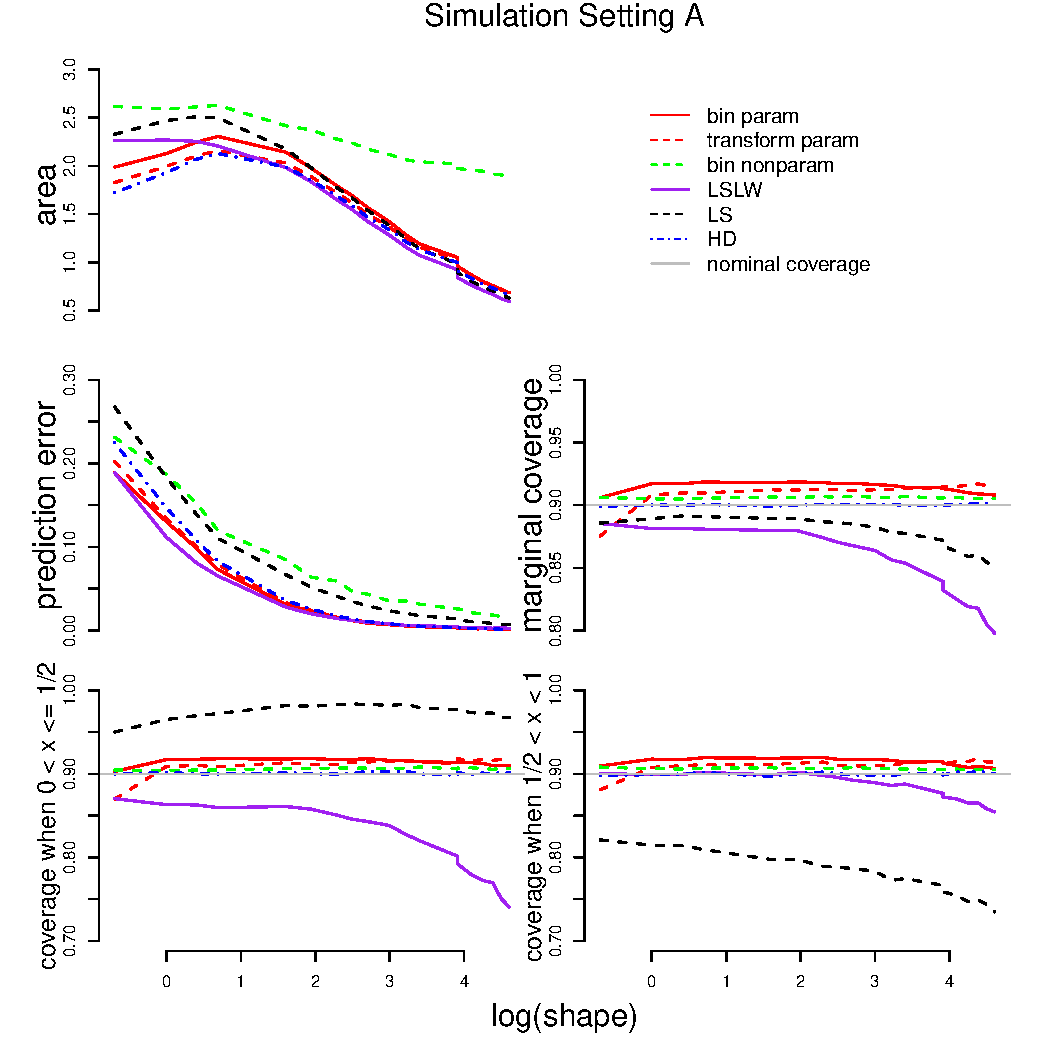
\includegraphics[width=\maxwidth]{figure/Fig-gamma-150-1} 

\end{knitrout}
\end{center}
\caption{This figure compares the performance of the 
  parametric,
  nonparametric,
  least squares, and 
  least squares locally weighted conformal prediciton region and the 
  highest density predcition region when $n = 150$ and the number of bins 
  equals 2.  
  The specific diagnostics used to compare these prediciton regions is the 
    area (top-left panel),
    prediction error (top-right panel), and
    the coverage probability with respect to binning (bottom row) 
    across shape parameter values.
  The average of 250 Monte Carlo samples at each shape parameter value in 
  these simulation settings form the lines that are depicted in this figure.}
\label{Fig:gamma.150}
\end{figure}


% local coverage, n = 150
\newpage
\begin{figure}[h!]
\begin{center}
\begin{knitrout}
\definecolor{shadecolor}{rgb}{0.969, 0.969, 0.969}\color{fgcolor}
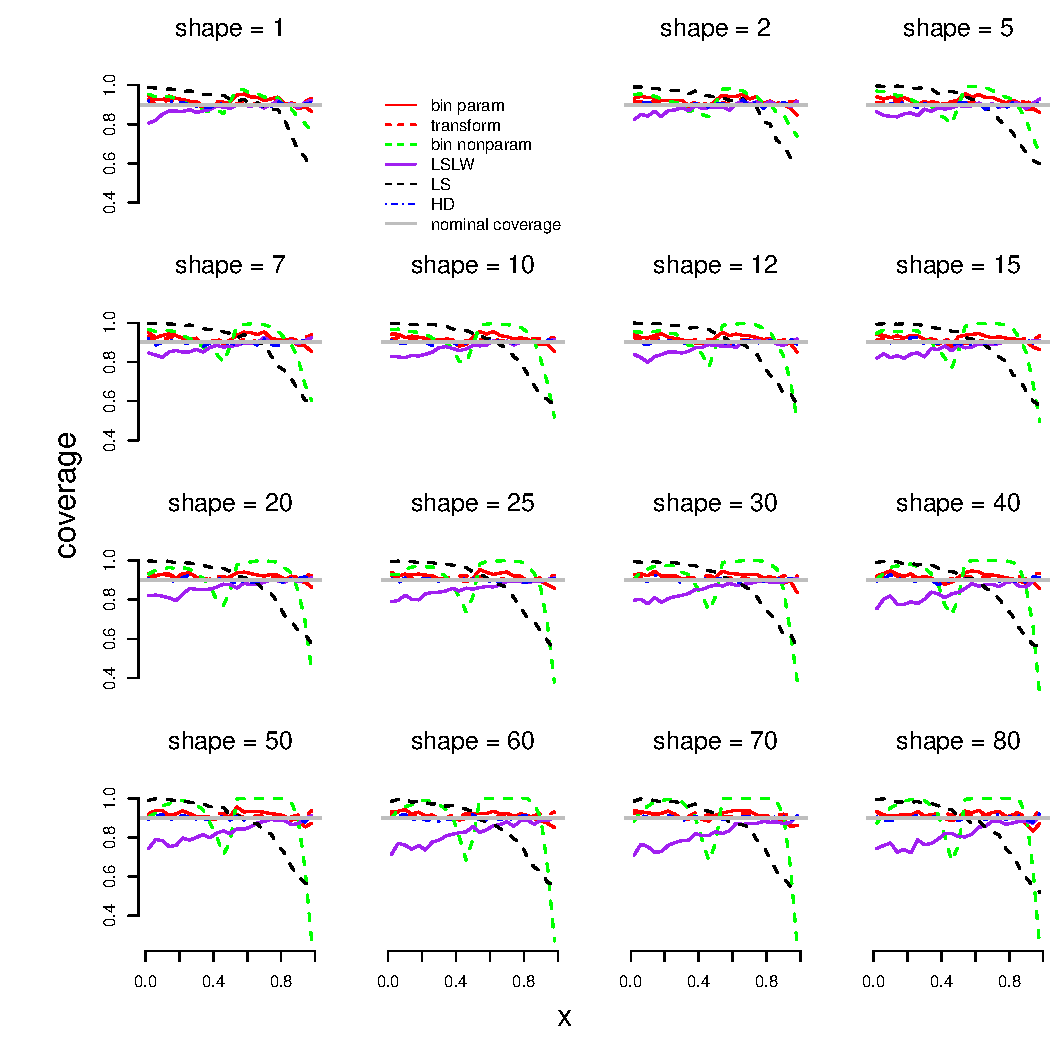
\includegraphics[width=\maxwidth]{figure/Fig-gamma-inx-150-1} 

\end{knitrout}
\end{center}
\caption{Plot of the estimated coverage probabilities of prediction regions 
  across $x$ and shape parameter values when the model is correctly 
  specified, $n = 150$, and the number of bins is equal to $2$.}
\label{Fig:gamma.inx.150}
\end{figure}


% Diagnostics, n = 250
\newpage
\begin{figure}[h!]
\begin{center}
\begin{knitrout}
\definecolor{shadecolor}{rgb}{0.969, 0.969, 0.969}\color{fgcolor}
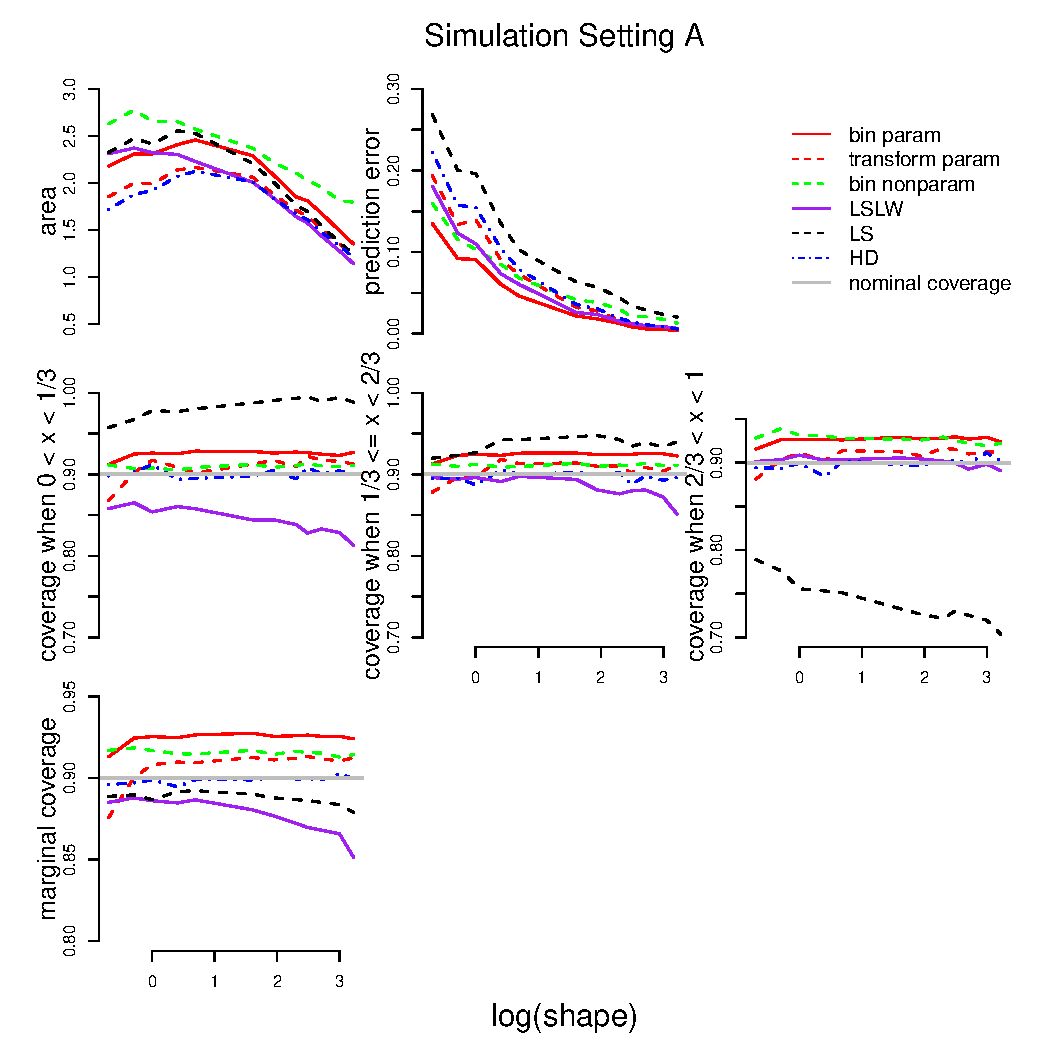
\includegraphics[width=\maxwidth]{figure/Fig-gamma-250-1} 

\end{knitrout}
\end{center}
\caption{This figure compares the performance of the 
  parametric,
  nonparametric,
  least squares, and 
  least squares locally weighted conformal prediciton region and the 
  highest density prediction region when $n = 250$ and the number of bins 
  equals 3.  
  The specific diagnostics used to compare these prediciton regions is the 
    area (top-left panel),
    prediction error (top-right panel), and
    the coverage probability with respect to binning (bottom row) 
    across shape parameter values.
  The average of 50 Monte Carlo samples at each shape parameter value in 
  these simulation settings form the lines that are depicted in this figure.}
\label{Fig:gamma.250}
\end{figure}



% local coverage, n = 250
\newpage
\begin{figure}[h!]
\begin{center}
\begin{knitrout}
\definecolor{shadecolor}{rgb}{0.969, 0.969, 0.969}\color{fgcolor}
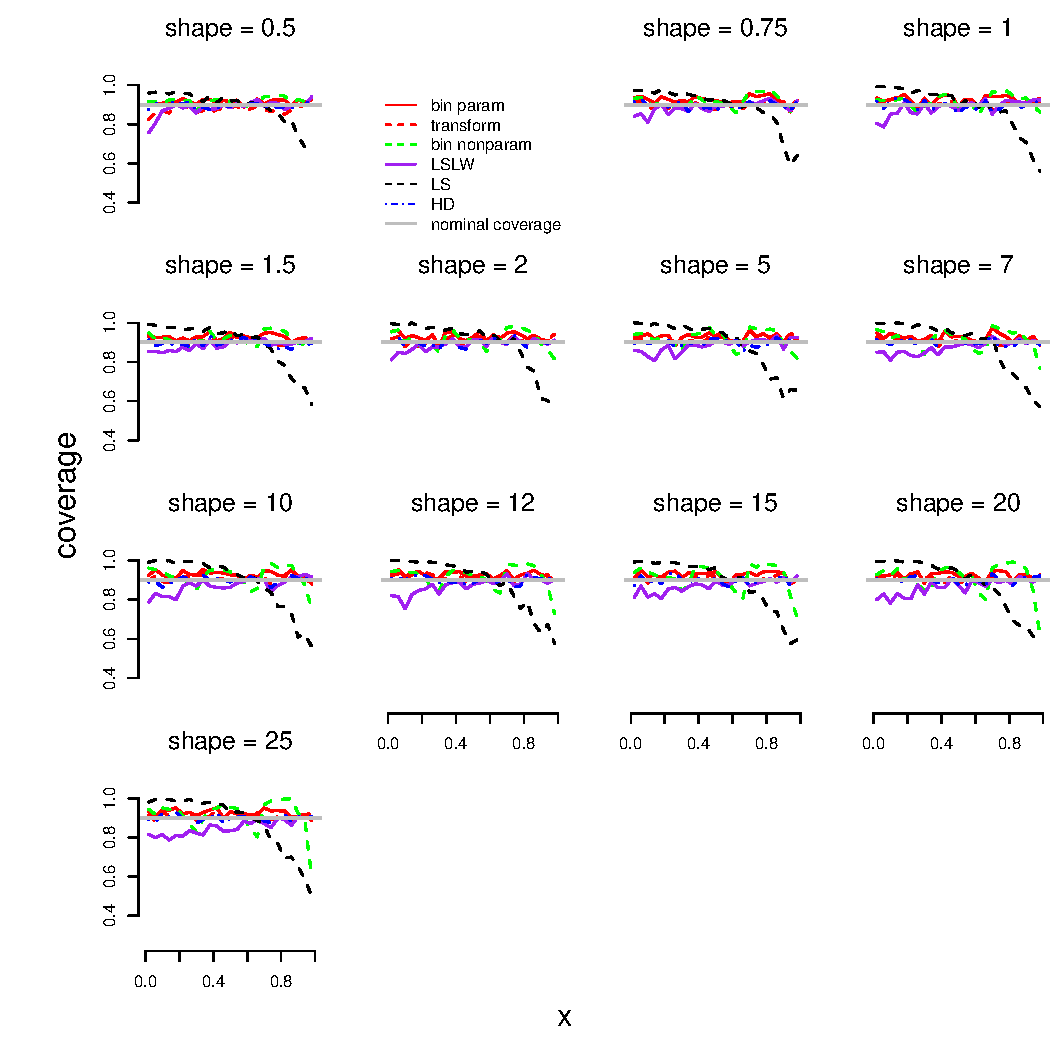
\includegraphics[width=\maxwidth]{figure/Fig-gamma-inx-250-1} 

\end{knitrout}
\end{center}
\caption{Plot of the estimated coverage probabilities of prediction regions 
  across $x$ and shape parameter values when the model is correctly 
  specified, $n = 250$, and the number of bins is equal to $3$.}
\label{Fig:gamma.inx.250}
\end{figure}



% Diagnostics, n = 500
\newpage
\begin{figure}[h!]
\begin{center}
\begin{knitrout}
\definecolor{shadecolor}{rgb}{0.969, 0.969, 0.969}\color{fgcolor}
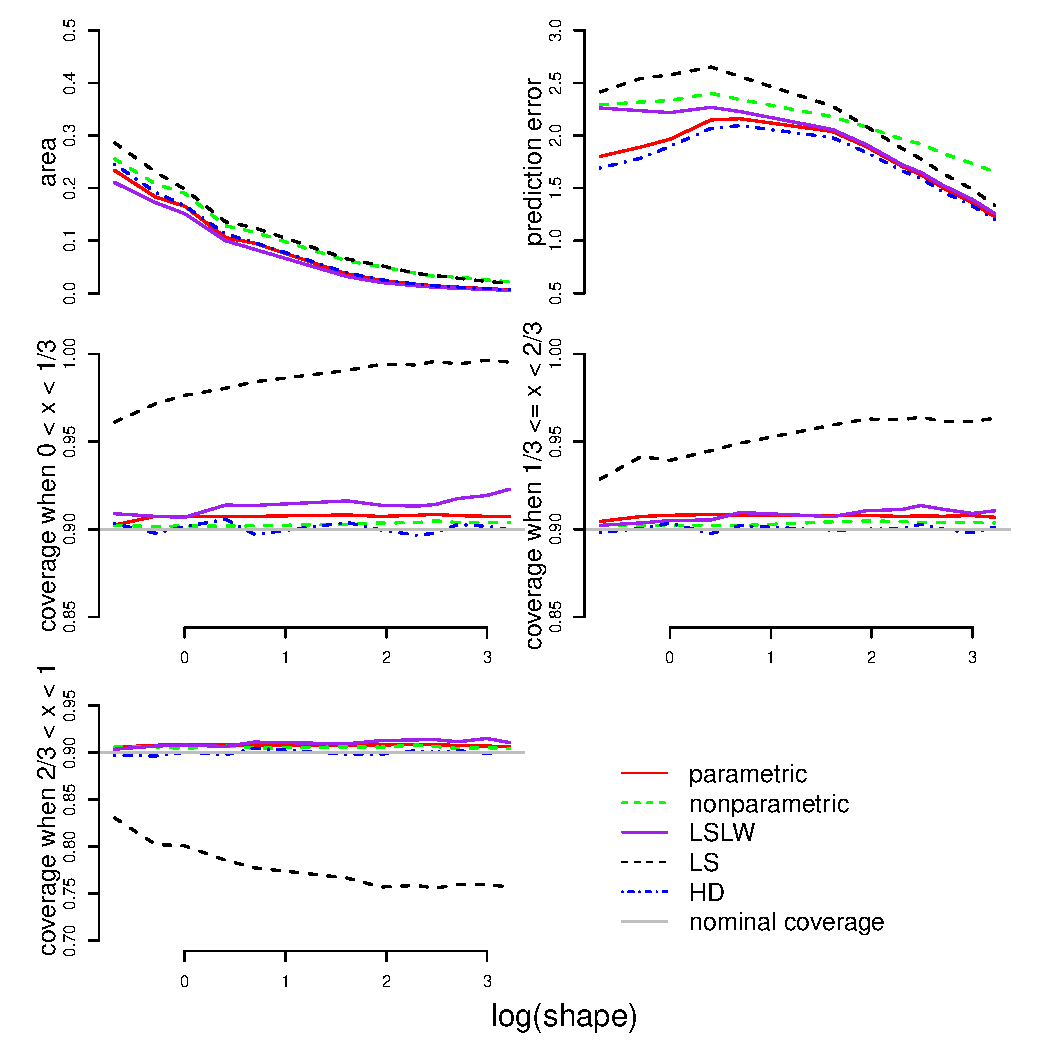
\includegraphics[width=\maxwidth]{figure/Fig-gamma-500-1} 

\end{knitrout}
\end{center}
\caption{Diagnostic plots for prediction regions when the model is correctly 
  specified, $n = 500$, and the number of bins is equal to $3$.}
\label{Fig:gamma.500}
\end{figure}



% local coverage, n = 500
\newpage
\begin{figure}[h!]
\begin{center}
\begin{knitrout}
\definecolor{shadecolor}{rgb}{0.969, 0.969, 0.969}\color{fgcolor}
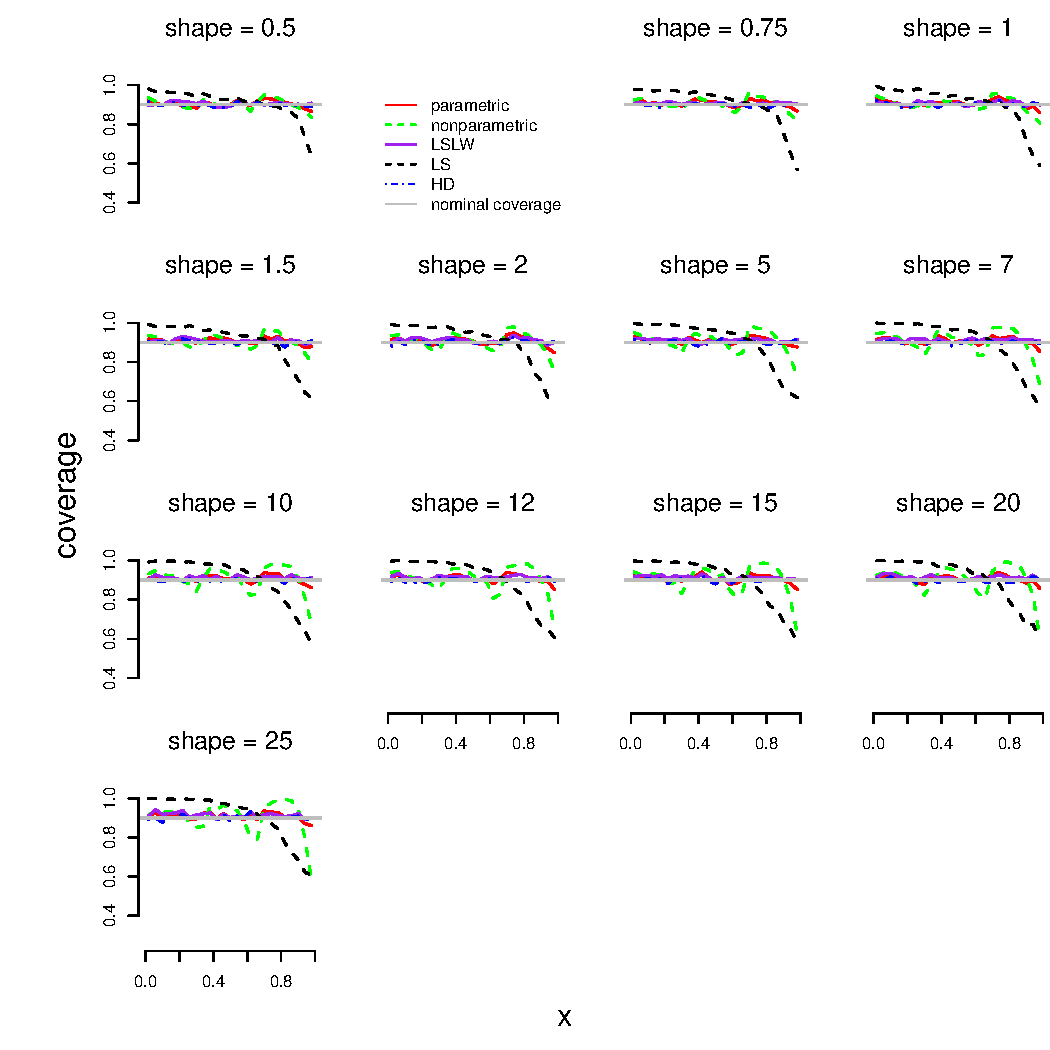
\includegraphics[width=\maxwidth]{figure/Fig-gamma-inx-500-1} 

\end{knitrout}
\end{center}
\caption{This figure compares the performance of the 
  parametric,
  nonparametric,
  least squares, and 
  least squares locally weighted conformal prediciton region and the 
  highest density prediction region when $n = 550$ and the number of bins 
  equals 3.  
  The specific diagnostics used to compare these prediciton regions is the 
    area (top-left panel),
    prediction error (top-right panel), and
    the coverage probability with respect to binning (bottom row) 
    across shape parameter values.
  The average of 50 Monte Carlo samples at each shape parameter value in 
  these simulation settings form the lines that are depicted in this figure.}
\label{Fig:gamma.inx.500}
\end{figure}







\newpage
\section{Gamma-Gaussian model misspecification}
\label{sec:misspec}

In this Section, we compare the parametric conformal prediction 
region, the nonparametric conformal prediction region, the LSLW conformal 
prediction region, the LS conformal prediction region, and the HD prediction 
region under model misspecification.  The data generating process is Gamma 
with an inverse link function and we set $\beta = (0.5, 1)^T$.
We consider sample sizes of $n \in \{150, 250, 500\}$ and shape parameter 
values of $\{5, 10, 20, 30, 40, 50, 60, 70, 80, 90, 100\}$ when $n = 150$ and 
shape parameter values of $\{5, 20, 40, 60, 80, 100\}$ when $n = 250, 500$.  
This value of $\beta$ and these shape parameter values are chosen so that 
errors about a cubic regression model appear to be almost symmetric.  In this 
analysis the parametric, LSLW, and LS conformal prediction regions and the HD 
prediction region are fit assuming this misspecified cubic regression model 
with homoscedastic normal errors.  When $n = 150$ we build the parametric and 
nonparametric conformal prediction regions using 2 bins.  When $n = 250, 500$ 
we build the parametric and nonparametric conformal prediction regions using 
3 bins.  These number of bin choices correspond to the bin width asymptotics 
of \citet{lei2014distribution}. 



\subsection{Simulations}

The following function computes our diagnostic measures for the five 
prediction regions under investigation in the univariate case where data 
is assumed to be Gamma with inverse link function and the fitted model is 
Gaussian with a cubic fit.  

\begin{knitrout}
\definecolor{shadecolor}{rgb}{0.969, 0.969, 0.969}\color{fgcolor}\begin{kframe}
\begin{alltt}
\hlstd{misspec.simulator} \hlkwb{<-} \hlkwa{function}\hlstd{(}\hlkwc{n} \hlstd{=} \hlnum{500}\hlstd{,} \hlkwc{alpha} \hlstd{=} \hlnum{0.10}\hlstd{,} \hlkwc{beta}\hlstd{,}
  \hlkwc{shape}\hlstd{,} \hlkwc{bins} \hlstd{=} \hlnum{3}\hlstd{,} \hlkwc{family} \hlstd{=} \hlstr{"Gamma"}\hlstd{,} \hlkwc{link} \hlstd{=} \hlstr{"inverse"}\hlstd{,}
  \hlkwc{confamily} \hlstd{=} \hlstr{"gaussian"}\hlstd{,} \hlkwc{parametric} \hlstd{=} \hlnum{TRUE}\hlstd{,}
  \hlkwc{nonparametric} \hlstd{=} \hlnum{TRUE}\hlstd{,} \hlkwc{LS} \hlstd{=} \hlnum{TRUE}\hlstd{,} \hlkwc{LSLW} \hlstd{=} \hlnum{TRUE}\hlstd{,} \hlkwc{HD} \hlstd{=} \hlnum{TRUE}\hlstd{,}
  \hlkwc{oracle} \hlstd{=} \hlnum{FALSE}\hlstd{,} \hlkwc{cores} \hlstd{=} \hlnum{6}\hlstd{)\{}

  \hlstd{p} \hlkwb{<-} \hlstd{d} \hlkwb{<-} \hlkwd{length}\hlstd{(beta)} \hlopt{-} \hlnum{1}
  \hlstd{x} \hlkwb{<-} \hlkwd{matrix}\hlstd{(}\hlkwd{runif}\hlstd{(n),} \hlkwc{ncol} \hlstd{= p)}
  \hlstd{y} \hlkwb{<-} \hlkwd{rep}\hlstd{(}\hlnum{0}\hlstd{,n)}
  \hlstd{data} \hlkwb{<-} \hlkwa{NULL}

  \hlcom{## set up partition}
  \hlkwa{if}\hlstd{(}\hlkwd{class}\hlstd{(bins)} \hlopt{==} \hlstr{"NULL"}\hlstd{)\{}
    \hlstd{wn} \hlkwb{<-} \hlkwd{min}\hlstd{(}\hlnum{1}\hlopt{/} \hlkwd{floor}\hlstd{(}\hlnum{1} \hlopt{/} \hlstd{(}\hlkwd{log}\hlstd{(n)}\hlopt{/}\hlstd{n)}\hlopt{^}\hlstd{(}\hlnum{1}\hlopt{/}\hlstd{(d}\hlopt{+}\hlnum{3}\hlstd{))),} \hlnum{1}\hlopt{/}\hlnum{2}\hlstd{)}
    \hlstd{bins} \hlkwb{<-} \hlnum{1} \hlopt{/} \hlstd{wn}
  \hlstd{\}}

  \hlcom{## generate the data (has functionality for different }
  \hlcom{## families and link functions)}
  \hlkwa{if}\hlstd{(family} \hlopt{==} \hlstr{"Gamma"}\hlstd{)\{}
    \hlkwa{if}\hlstd{(link} \hlopt{==} \hlstr{"identity"}\hlstd{)\{}
      \hlstd{rate} \hlkwb{<-} \hlstd{(}\hlnum{1} \hlopt{/} \hlstd{(}\hlkwd{cbind}\hlstd{(}\hlnum{1}\hlstd{, x)} \hlopt \hlstd{beta))} \hlopt{*} \hlstd{shape}
      \hlstd{y} \hlkwb{<-} \hlkwd{rgamma}\hlstd{(}\hlkwc{n} \hlstd{= n,} \hlkwc{shape} \hlstd{= shape,} \hlkwc{rate} \hlstd{= rate)}
      \hlstd{y} \hlkwb{<-} \hlstd{y} \hlopt{/} \hlkwd{sd}\hlstd{(y)}
      \hlstd{data} \hlkwb{<-} \hlkwd{data.frame}\hlstd{(}\hlkwc{y} \hlstd{= y,} \hlkwc{x} \hlstd{= x)}
      \hlkwd{colnames}\hlstd{(data)[}\hlnum{2}\hlopt{:}\hlstd{(p}\hlopt{+}\hlnum{1}\hlstd{)]} \hlkwb{<-} \hlkwd{paste}\hlstd{(}\hlstr{"x"}\hlstd{,} \hlnum{1}\hlopt{:}\hlstd{p,} \hlkwc{sep} \hlstd{=} \hlstr{""}\hlstd{)}
    \hlstd{\}}
    \hlkwa{if}\hlstd{(link} \hlopt{==} \hlstr{"inverse"}\hlstd{)\{}
      \hlstd{rate} \hlkwb{<-} \hlstd{(}\hlkwd{cbind}\hlstd{(}\hlnum{1}\hlstd{, x)} \hlopt \hlstd{beta)} \hlopt{*} \hlstd{shape}
      \hlstd{y} \hlkwb{<-} \hlkwd{rgamma}\hlstd{(}\hlkwc{n} \hlstd{= n,} \hlkwc{shape} \hlstd{= shape,} \hlkwc{rate} \hlstd{= rate)}
      \hlstd{y} \hlkwb{<-} \hlstd{y} \hlopt{/} \hlkwd{sd}\hlstd{(y)}
      \hlstd{data} \hlkwb{<-} \hlkwd{data.frame}\hlstd{(}\hlkwc{y} \hlstd{= y,} \hlkwc{x} \hlstd{= x)}
      \hlkwd{colnames}\hlstd{(data)[}\hlnum{2}\hlopt{:}\hlstd{(p}\hlopt{+}\hlnum{1}\hlstd{)]} \hlkwb{<-} \hlkwd{paste}\hlstd{(}\hlstr{"x"}\hlstd{,} \hlnum{1}\hlopt{:}\hlstd{p,} \hlkwc{sep} \hlstd{=} \hlstr{""}\hlstd{)}
    \hlstd{\}}
    \hlkwa{if}\hlstd{(link} \hlopt{==} \hlstr{"log"}\hlstd{)\{}
      \hlstd{rate} \hlkwb{<-} \hlstd{(}\hlnum{1} \hlopt{/} \hlkwd{exp}\hlstd{(}\hlkwd{cbind}\hlstd{(}\hlnum{1}\hlstd{, x)} \hlopt \hlstd{beta))} \hlopt{*} \hlstd{shape}
      \hlstd{y} \hlkwb{<-} \hlkwd{rgamma}\hlstd{(}\hlkwc{n} \hlstd{= n,} \hlkwc{shape} \hlstd{= shape,} \hlkwc{rate} \hlstd{= rate)}
      \hlstd{y} \hlkwb{<-} \hlstd{y} \hlopt{/} \hlkwd{sd}\hlstd{(y)}
      \hlstd{data} \hlkwb{<-} \hlkwd{data.frame}\hlstd{(}\hlkwc{y} \hlstd{= y,} \hlkwc{x} \hlstd{= x)}
      \hlkwd{colnames}\hlstd{(data)[}\hlnum{2}\hlopt{:}\hlstd{(p}\hlopt{+}\hlnum{1}\hlstd{)]} \hlkwb{<-} \hlkwd{paste}\hlstd{(}\hlstr{"x"}\hlstd{,} \hlnum{1}\hlopt{:}\hlstd{p,} \hlkwc{sep} \hlstd{=} \hlstr{""}\hlstd{)}
    \hlstd{\}}
  \hlstd{\}}

  \hlkwa{if}\hlstd{(family} \hlopt{==} \hlstr{"gaussian"}\hlstd{)\{}
    \hlstd{mu} \hlkwb{<-} \hlkwd{cbind}\hlstd{(}\hlnum{1}\hlstd{, x)} \hlopt \hlstd{beta}
    \hlstd{y} \hlkwb{<-} \hlkwd{rnorm}\hlstd{(}\hlkwc{n} \hlstd{= n,} \hlkwc{mean} \hlstd{= mu,} \hlkwc{sd} \hlstd{= sd)}
    \hlstd{data} \hlkwb{<-} \hlkwd{data.frame}\hlstd{(}\hlkwc{y} \hlstd{= y,} \hlkwc{x} \hlstd{= x)}
    \hlkwd{colnames}\hlstd{(data)[}\hlnum{2}\hlopt{:}\hlstd{(p}\hlopt{+}\hlnum{1}\hlstd{)]} \hlkwb{<-} \hlkwd{paste}\hlstd{(}\hlstr{"x"}\hlstd{,} \hlnum{1}\hlopt{:}\hlstd{p,} \hlkwc{sep} \hlstd{=} \hlstr{""}\hlstd{)}
  \hlstd{\}}

  \hlkwa{if}\hlstd{(family} \hlopt{==} \hlstr{"inverse.gaussian"}\hlstd{)\{}
    \hlstd{mu} \hlkwb{=} \hlnum{1} \hlopt{/} \hlkwd{sqrt}\hlstd{(}\hlkwd{cbind}\hlstd{(}\hlnum{1}\hlstd{, x)} \hlopt \hlstd{beta)}
    \hlstd{y} \hlkwb{<-} \hlkwd{rinvgauss}\hlstd{(}\hlkwc{n} \hlstd{= n,} \hlkwc{mean} \hlstd{= mu)}
    \hlstd{y} \hlkwb{<-} \hlstd{y} \hlopt{/} \hlkwd{sd}\hlstd{(y)}
    \hlstd{data} \hlkwb{<-} \hlkwd{data.frame}\hlstd{(}\hlkwc{y} \hlstd{= y,} \hlkwc{x} \hlstd{= x)}
    \hlkwd{colnames}\hlstd{(data)[}\hlnum{2}\hlopt{:}\hlstd{(p}\hlopt{+}\hlnum{1}\hlstd{)]} \hlkwb{<-} \hlkwd{paste}\hlstd{(}\hlstr{"x"}\hlstd{,} \hlnum{1}\hlopt{:}\hlstd{p,} \hlkwc{sep} \hlstd{=} \hlstr{""}\hlstd{)}
  \hlstd{\}}

  \hlcom{## fit the misspecified cubic regression model}
  \hlstd{fit} \hlkwb{<-} \hlkwd{glm}\hlstd{(y} \hlopt{~} \hlstd{x1} \hlopt{+} \hlkwd{I}\hlstd{(x1}\hlopt{^}\hlnum{2}\hlstd{)} \hlopt{+} \hlkwd{I}\hlstd{(x1}\hlopt{^}\hlnum{3}\hlstd{),} \hlkwc{family} \hlstd{= confamily,}
    \hlkwc{data} \hlstd{= data)}
  \hlstd{paraCI} \hlkwb{<-} \hlstd{nonparaCI} \hlkwb{<-} \hlstd{LSCI} \hlkwb{<-} \hlstd{LSLWCI} \hlkwb{<-} \hlstd{HDCI} \hlkwb{<-}
    \hlstd{trueHDCI} \hlkwb{<-} \hlkwa{NULL}
  \hlstd{formula} \hlkwb{<-} \hlstd{fit}\hlopt{$}\hlstd{formula}
  \hlstd{newdata} \hlkwb{<-} \hlstd{data}
  \hlstd{respname} \hlkwb{<-} \hlkwd{all.vars}\hlstd{(formula)[}\hlnum{1}\hlstd{]}
  \hlstd{newdata} \hlkwb{<-} \hlstd{newdata[,} \hlopt{!}\hlstd{(}\hlkwd{colnames}\hlstd{(data)} \hlopt \hlstd{respname)]}
  \hlstd{newdata} \hlkwb{<-} \hlkwd{as.matrix}\hlstd{(newdata)}

  \hlcom{## obtain the prediction regions}
  \hlkwa{if}\hlstd{(parametric)\{}
    \hlstd{cpred} \hlkwb{<-} \hlkwd{conformal.glm}\hlstd{(fit,} \hlkwc{parametric} \hlstd{=} \hlnum{TRUE}\hlstd{,}
      \hlkwc{nonparametric} \hlstd{=} \hlnum{FALSE}\hlstd{,} \hlkwc{alpha} \hlstd{= alpha,}
      \hlkwc{bins} \hlstd{= bins,} \hlkwc{cores} \hlstd{= cores)}
    \hlstd{paraCI} \hlkwb{<-} \hlstd{cpred}\hlopt{$}\hlstd{paraconformal}
  \hlstd{\}}
  \hlkwa{if}\hlstd{(nonparametric)\{}
    \hlstd{cpred} \hlkwb{<-} \hlkwd{conformal.glm}\hlstd{(fit,} \hlkwc{parametric} \hlstd{=} \hlnum{FALSE}\hlstd{,}
      \hlkwc{nonparametric} \hlstd{=} \hlnum{TRUE}\hlstd{,} \hlkwc{alpha} \hlstd{= alpha,}
      \hlkwc{bins} \hlstd{= bins,} \hlkwc{cores} \hlstd{= cores)}
    \hlstd{nonparaCI} \hlkwb{<-} \hlstd{cpred}\hlopt{$}\hlstd{nonparaconformal}
  \hlstd{\}}
  \hlkwa{if}\hlstd{(LS)\{}
    \hlstd{p1.tibs} \hlkwb{<-} \hlkwd{conformal.pred}\hlstd{(}\hlkwc{x} \hlstd{=} \hlkwd{cbind}\hlstd{(x,x}\hlopt{^}\hlnum{2}\hlstd{,x}\hlopt{^}\hlnum{3}\hlstd{),} \hlkwc{y} \hlstd{= y,}
      \hlkwc{x0} \hlstd{=} \hlkwd{cbind}\hlstd{(x,x}\hlopt{^}\hlnum{2}\hlstd{,x}\hlopt{^}\hlnum{3}\hlstd{),}
      \hlkwc{train.fun} \hlstd{= train.fun,} \hlkwc{predict.fun} \hlstd{= predict.fun,}
      \hlkwc{alpha} \hlstd{= alpha)}
    \hlstd{LSCI} \hlkwb{<-} \hlkwd{cbind}\hlstd{(p1.tibs}\hlopt{$}\hlstd{lo, p1.tibs}\hlopt{$}\hlstd{up)}
  \hlstd{\}}
  \hlkwa{if}\hlstd{(LSLW)\{}
    \hlstd{cubic.model} \hlkwb{<-} \hlkwd{lm}\hlstd{(y} \hlopt{~} \hlstd{x} \hlopt{+} \hlkwd{I}\hlstd{(x}\hlopt{^}\hlnum{2}\hlstd{)} \hlopt{+} \hlkwd{I}\hlstd{(x}\hlopt{^}\hlnum{3}\hlstd{))}
    \hlstd{abs.resid} \hlkwb{<-} \hlkwd{abs}\hlstd{(cubic.model}\hlopt{$}\hlstd{resid)}
    \hlstd{smooth.call} \hlkwb{<-} \hlkwd{smooth.spline}\hlstd{(x, abs.resid,}
      \hlkwc{nknots} \hlstd{=} \hlnum{10}\hlstd{)}
    \hlstd{lambda} \hlkwb{<-} \hlstd{smooth.call}\hlopt{$}\hlstd{lambda}
    \hlstd{df} \hlkwb{<-} \hlstd{smooth.call}\hlopt{$}\hlstd{df}
    \hlstd{mad.train.fun} \hlkwb{<-} \hlkwa{function}\hlstd{(}\hlkwc{x}\hlstd{,} \hlkwc{y}\hlstd{,} \hlkwc{out} \hlstd{=} \hlkwa{NULL}\hlstd{)\{}
      \hlkwd{smooth.spline}\hlstd{(x[,} \hlnum{1}\hlstd{], y,} \hlkwc{lambda} \hlstd{= lambda,}
      \hlkwc{df} \hlstd{= df,} \hlkwc{nknots} \hlstd{=} \hlnum{10}\hlstd{)}
    \hlstd{\}}
    \hlstd{p2.tibs} \hlkwb{<-} \hlkwd{conformal.pred}\hlstd{(}\hlkwc{x} \hlstd{=} \hlkwd{cbind}\hlstd{(x,x}\hlopt{^}\hlnum{2}\hlstd{,x}\hlopt{^}\hlnum{3}\hlstd{),} \hlkwc{y} \hlstd{= y,}
      \hlkwc{x0} \hlstd{=} \hlkwd{cbind}\hlstd{(x,x}\hlopt{^}\hlnum{2}\hlstd{,x}\hlopt{^}\hlnum{3}\hlstd{),}
      \hlkwc{train.fun} \hlstd{= train.fun,} \hlkwc{predict.fun} \hlstd{= predict.fun,}
      \hlkwc{mad.train.fun} \hlstd{= mad.train.fun,}
      \hlkwc{mad.predict.fun} \hlstd{= mad.predict.fun,}
      \hlkwc{alpha} \hlstd{= alpha)}
    \hlstd{LSLWCI} \hlkwb{<-} \hlkwd{cbind}\hlstd{(p2.tibs}\hlopt{$}\hlstd{lo, p2.tibs}\hlopt{$}\hlstd{up)}
  \hlstd{\}}
  \hlkwa{if}\hlstd{(HD)\{}
    \hlkwa{if}\hlstd{(oracle)\{}
      \hlstd{fit.gamma} \hlkwb{<-} \hlkwd{glm}\hlstd{(y} \hlopt{~} \hlstd{x1,} \hlkwc{family} \hlstd{=} \hlstr{"Gamma"}\hlstd{,} \hlkwc{data} \hlstd{= data)}
      \hlstd{betaMLE} \hlkwb{<-} \hlkwd{coefficients}\hlstd{(fit.gamma)}
      \hlstd{shapeMLE} \hlkwb{<-} \hlkwd{as.numeric}\hlstd{(}\hlkwd{gamma.shape}\hlstd{(fit.gamma)[}\hlnum{1}\hlstd{])}
      \hlstd{rateMLE} \hlkwb{<-} \hlkwd{cbind}\hlstd{(}\hlnum{1}\hlstd{, newdata)} \hlopt \hlstd{betaMLE} \hlopt{*} \hlstd{shapeMLE}
      \hlstd{trueHDCI} \hlkwb{<-} \hlkwd{do.call}\hlstd{(rbind,} \hlkwd{lapply}\hlstd{(}\hlnum{1}\hlopt{:}\hlkwd{nrow}\hlstd{(newdata),} \hlkwa{function}\hlstd{(}\hlkwc{j}\hlstd{)\{}
        \hlkwd{hdi}\hlstd{(qgamma,} \hlnum{1} \hlopt{-} \hlstd{alpha,} \hlkwc{shape} \hlstd{= shapeMLE,} \hlkwc{rate} \hlstd{= rateMLE[j,} \hlnum{1}\hlstd{])}
      \hlstd{\}))}
    \hlstd{\}}
    \hlstd{fit} \hlkwb{=} \hlkwd{lm}\hlstd{(y} \hlopt{~} \hlstd{x1} \hlopt{+} \hlkwd{I}\hlstd{(x1}\hlopt{^}\hlnum{2}\hlstd{)} \hlopt{+} \hlkwd{I}\hlstd{(x1}\hlopt{^}\hlnum{3}\hlstd{),} \hlkwc{data} \hlstd{= data)}
    \hlstd{betaMLE} \hlkwb{<-} \hlkwd{coefficients}\hlstd{(fit)}
    \hlstd{sdMLE} \hlkwb{<-} \hlkwd{summary}\hlstd{(fit)}\hlopt{$}\hlstd{sigma}
    \hlstd{meanMLE} \hlkwb{<-} \hlkwd{as.numeric}\hlstd{(}\hlkwd{cbind}\hlstd{(}\hlnum{1}\hlstd{, x, x}\hlopt{^}\hlnum{2}\hlstd{, x}\hlopt{^}\hlnum{3}\hlstd{)} \hlopt \hlstd{betaMLE)}
    \hlstd{HDCI} \hlkwb{<-} \hlkwd{do.call}\hlstd{(rbind,} \hlkwd{lapply}\hlstd{(}\hlnum{1}\hlopt{:}\hlkwd{nrow}\hlstd{(newdata),} \hlkwa{function}\hlstd{(}\hlkwc{j}\hlstd{)\{}
      \hlkwd{hdi}\hlstd{(qnorm,} \hlnum{1} \hlopt{-} \hlstd{alpha,} \hlkwc{sd} \hlstd{= sdMLE,} \hlkwc{mean} \hlstd{= meanMLE[j])}
    \hlstd{\}))}
  \hlstd{\}}

  \hlcom{## local coverage prediction regions}
  \hlstd{output.parametric} \hlkwb{<-} \hlstd{output.nonparametric} \hlkwb{<-}
    \hlstd{output.LS} \hlkwb{<-} \hlstd{output.LSLW} \hlkwb{<-} \hlstd{output.HD} \hlkwb{<-}
    \hlstd{output.trueHD} \hlkwb{<-} \hlkwd{rep}\hlstd{(}\hlnum{NA}\hlstd{, bins} \hlopt{+} \hlnum{1}\hlstd{)}
  \hlkwa{if}\hlstd{(parametric)\{}
    \hlstd{marginal.parametric} \hlkwb{<-} \hlkwd{local.coverage}\hlstd{(}\hlkwc{region} \hlstd{= paraCI,}
      \hlkwc{data} \hlstd{= data,} \hlkwc{d} \hlstd{= p,} \hlkwc{bins} \hlstd{=} \hlnum{1}\hlstd{,} \hlkwc{at.data} \hlstd{=} \hlstr{"TRUE"}\hlstd{)}
    \hlstd{local.parametric} \hlkwb{<-} \hlkwd{local.coverage}\hlstd{(}\hlkwc{region} \hlstd{= paraCI,}
      \hlkwc{data} \hlstd{= data,} \hlkwc{d} \hlstd{= p,} \hlkwc{bins} \hlstd{= bins,} \hlkwc{at.data} \hlstd{=} \hlstr{"TRUE"}\hlstd{)}
    \hlstd{local.inx.parametric} \hlkwb{<-} \hlkwd{local.coverage}\hlstd{(}\hlkwc{region} \hlstd{= paraCI,}
      \hlkwc{data} \hlstd{= data,} \hlkwc{d} \hlstd{= p,} \hlkwc{bins} \hlstd{=} \hlnum{25}\hlstd{,} \hlkwc{at.data} \hlstd{=} \hlstr{"TRUE"}\hlstd{)}
    \hlstd{output.parametric} \hlkwb{<-} \hlkwd{c}\hlstd{(marginal.parametric, local.parametric,}
      \hlstd{local.inx.parametric,}
      \hlkwd{mean}\hlstd{(}\hlkwd{apply}\hlstd{(paraCI,} \hlnum{1}\hlstd{, diff)),}
      \hlkwd{absolute.error}\hlstd{(}\hlkwc{y} \hlstd{= y,} \hlkwc{region} \hlstd{= paraCI))}
  \hlstd{\}}
  \hlkwa{if}\hlstd{(nonparametric)\{}
    \hlstd{marginal.nonparametric} \hlkwb{<-} \hlkwd{local.coverage}\hlstd{(}\hlkwc{region} \hlstd{= nonparaCI,}
      \hlkwc{nonparametric} \hlstd{=} \hlstr{"TRUE"}\hlstd{,} \hlkwc{data} \hlstd{= data,} \hlkwc{d} \hlstd{= p,} \hlkwc{bins} \hlstd{=} \hlnum{1}\hlstd{,}
      \hlkwc{at.data} \hlstd{=} \hlstr{"TRUE"}\hlstd{)}
    \hlstd{local.nonparametric} \hlkwb{<-} \hlkwd{local.coverage}\hlstd{(}\hlkwc{region} \hlstd{= nonparaCI,}
      \hlkwc{nonparametric} \hlstd{=} \hlstr{"TRUE"}\hlstd{,} \hlkwc{data} \hlstd{= data,} \hlkwc{d} \hlstd{= p,} \hlkwc{bins} \hlstd{= bins,}
      \hlkwc{at.data} \hlstd{=} \hlstr{"TRUE"}\hlstd{)}
    \hlstd{local.inx.nonparametric} \hlkwb{<-} \hlkwd{local.coverage}\hlstd{(}\hlkwc{region} \hlstd{= nonparaCI,}
      \hlkwc{nonparametric} \hlstd{=} \hlstr{"TRUE"}\hlstd{,} \hlkwc{data} \hlstd{= data,} \hlkwc{d} \hlstd{= p,} \hlkwc{bins} \hlstd{=} \hlnum{25}\hlstd{,}
      \hlkwc{at.data} \hlstd{=} \hlstr{"TRUE"}\hlstd{)}
    \hlstd{output.nonparametric} \hlkwb{<-}
      \hlkwd{c}\hlstd{(marginal.nonparametric, local.nonparametric,}
        \hlstd{local.inx.nonparametric,}
        \hlkwd{area.nonparametric}\hlstd{(nonparaCI),}
        \hlkwd{absolute.error.nonparametric}\hlstd{(}\hlkwc{data} \hlstd{= data,}
          \hlkwc{region} \hlstd{= nonparaCI))}
  \hlstd{\}}
  \hlkwa{if}\hlstd{(LS)\{}
    \hlstd{marginal.LS} \hlkwb{<-} \hlkwd{local.coverage}\hlstd{(}\hlkwc{region} \hlstd{= LSCI,}
      \hlkwc{data} \hlstd{= data,} \hlkwc{d} \hlstd{= p,} \hlkwc{bins} \hlstd{=} \hlnum{1}\hlstd{,} \hlkwc{at.data} \hlstd{=} \hlstr{"TRUE"}\hlstd{)}
    \hlstd{local.LS} \hlkwb{<-} \hlkwd{local.coverage}\hlstd{(}\hlkwc{region} \hlstd{= LSCI,}
      \hlkwc{data} \hlstd{= data,} \hlkwc{d} \hlstd{= p,} \hlkwc{bins} \hlstd{= bins,} \hlkwc{at.data} \hlstd{=} \hlstr{"TRUE"}\hlstd{)}
    \hlstd{local.inx.LS} \hlkwb{<-} \hlkwd{local.coverage}\hlstd{(}\hlkwc{region} \hlstd{= LSCI,}
      \hlkwc{data} \hlstd{= data,} \hlkwc{d} \hlstd{= p,} \hlkwc{bins} \hlstd{=} \hlnum{25}\hlstd{,} \hlkwc{at.data} \hlstd{=} \hlstr{"TRUE"}\hlstd{)}
    \hlstd{output.LS} \hlkwb{<-} \hlkwd{c}\hlstd{(marginal.LS, local.LS, local.inx.LS,}
      \hlkwd{mean}\hlstd{(}\hlkwd{apply}\hlstd{(LSCI,} \hlnum{1}\hlstd{, diff)),}
      \hlkwd{absolute.error}\hlstd{(}\hlkwc{y} \hlstd{= y,} \hlkwc{region} \hlstd{= LSCI))}
  \hlstd{\}}
  \hlkwa{if}\hlstd{(LSLW)\{}
    \hlstd{marginal.LSLW} \hlkwb{<-} \hlkwd{local.coverage}\hlstd{(}\hlkwc{region} \hlstd{= LSLWCI,}
      \hlkwc{data} \hlstd{= data,} \hlkwc{d} \hlstd{= p,} \hlkwc{bins} \hlstd{=} \hlnum{1}\hlstd{,} \hlkwc{at.data} \hlstd{=} \hlstr{"TRUE"}\hlstd{)}
    \hlstd{local.LSLW} \hlkwb{<-} \hlkwd{local.coverage}\hlstd{(}\hlkwc{region} \hlstd{= LSLWCI,}
      \hlkwc{data} \hlstd{= data,} \hlkwc{d} \hlstd{= p,} \hlkwc{bins} \hlstd{= bins,} \hlkwc{at.data} \hlstd{=} \hlstr{"TRUE"}\hlstd{)}
    \hlstd{local.inx.LSLW} \hlkwb{<-} \hlkwd{local.coverage}\hlstd{(}\hlkwc{region} \hlstd{= LSLWCI,}
      \hlkwc{data} \hlstd{= data,} \hlkwc{d} \hlstd{= p,} \hlkwc{bins} \hlstd{=} \hlnum{25}\hlstd{,} \hlkwc{at.data} \hlstd{=} \hlstr{"TRUE"}\hlstd{)}
    \hlstd{output.LSLW} \hlkwb{<-} \hlkwd{c}\hlstd{(marginal.LSLW, local.LSLW, local.inx.LSLW,}
      \hlkwd{mean}\hlstd{(}\hlkwd{apply}\hlstd{(LSLWCI,} \hlnum{1}\hlstd{, diff)),}
      \hlkwd{absolute.error}\hlstd{(}\hlkwc{y} \hlstd{= y,} \hlkwc{region} \hlstd{= LSLWCI))}
  \hlstd{\}}
  \hlkwa{if}\hlstd{(HD)\{}
    \hlstd{marginal.HD} \hlkwb{<-} \hlkwd{local.coverage}\hlstd{(}\hlkwc{region} \hlstd{= HDCI,}
      \hlkwc{data} \hlstd{= data,} \hlkwc{d} \hlstd{= p,} \hlkwc{bins} \hlstd{=} \hlnum{1}\hlstd{,} \hlkwc{at.data} \hlstd{=} \hlstr{"TRUE"}\hlstd{)}
    \hlstd{local.HD} \hlkwb{<-} \hlkwd{local.coverage}\hlstd{(}\hlkwc{region} \hlstd{= HDCI,}
      \hlkwc{data} \hlstd{= data,} \hlkwc{d} \hlstd{= p,} \hlkwc{bins} \hlstd{= bins,} \hlkwc{at.data} \hlstd{=} \hlstr{"TRUE"}\hlstd{)}
    \hlstd{local.inx.HD} \hlkwb{<-} \hlkwd{local.coverage}\hlstd{(}\hlkwc{region} \hlstd{= HDCI,}
      \hlkwc{data} \hlstd{= data,} \hlkwc{d} \hlstd{= p,} \hlkwc{bins} \hlstd{=} \hlnum{25}\hlstd{,} \hlkwc{at.data} \hlstd{=} \hlstr{"TRUE"}\hlstd{)}
    \hlstd{output.HD} \hlkwb{<-} \hlkwd{c}\hlstd{(marginal.HD, local.HD, local.inx.HD,}
      \hlkwd{mean}\hlstd{(}\hlkwd{apply}\hlstd{(HDCI,} \hlnum{1}\hlstd{, diff)),}
      \hlkwd{absolute.error}\hlstd{(}\hlkwc{y} \hlstd{= y,} \hlkwc{region} \hlstd{= HDCI))}
    \hlkwa{if}\hlstd{(oracle)\{}
      \hlstd{marginal.trueHD} \hlkwb{<-} \hlkwd{local.coverage}\hlstd{(}\hlkwc{region} \hlstd{= trueHDCI,}
        \hlkwc{data} \hlstd{= data,} \hlkwc{d} \hlstd{= p,} \hlkwc{bins} \hlstd{=} \hlnum{1}\hlstd{,} \hlkwc{at.data} \hlstd{=} \hlstr{"TRUE"}\hlstd{)}
      \hlstd{local.trueHD} \hlkwb{<-} \hlkwd{local.coverage}\hlstd{(}\hlkwc{region} \hlstd{= trueHDCI,}
        \hlkwc{data} \hlstd{= data,} \hlkwc{d} \hlstd{= p,} \hlkwc{bins} \hlstd{= bins,} \hlkwc{at.data} \hlstd{=} \hlstr{"TRUE"}\hlstd{)}
      \hlstd{local.inx.trueHD} \hlkwb{<-} \hlkwd{local.coverage}\hlstd{(}\hlkwc{region} \hlstd{= trueHDCI,}
        \hlkwc{data} \hlstd{= data,} \hlkwc{d} \hlstd{= p,} \hlkwc{bins} \hlstd{=} \hlnum{25}\hlstd{,} \hlkwc{at.data} \hlstd{=} \hlstr{"TRUE"}\hlstd{)}
      \hlstd{output.trueHD} \hlkwb{<-} \hlkwd{c}\hlstd{(marginal.trueHD, local.trueHD,}
        \hlstd{local.inx.trueHD,} \hlkwd{mean}\hlstd{(}\hlkwd{apply}\hlstd{(trueHDCI,} \hlnum{1}\hlstd{, diff)),}
        \hlkwd{absolute.error}\hlstd{(}\hlkwc{y} \hlstd{= y,} \hlkwc{region} \hlstd{= trueHDCI))}
    \hlstd{\}}
  \hlstd{\}}

  \hlstd{output} \hlkwb{<-} \hlkwd{list}\hlstd{(}\hlkwc{output.parametric} \hlstd{= output.parametric,}
    \hlkwc{output.nonparametric} \hlstd{= output.nonparametric,}
    \hlkwc{output.LS} \hlstd{= output.LS,}
    \hlkwc{output.LSLW} \hlstd{= output.LSLW,}
    \hlkwc{output.HD} \hlstd{= output.HD,}
    \hlkwc{output.trueHD} \hlstd{= output.trueHD)}
  \hlstd{output}

\hlstd{\}}
\end{alltt}
\end{kframe}
\end{knitrout}

%The following performs our Monte Carlo simulation of $B = 250$ iterations 
%when $n = 150$ and shape = $0.5$.

%<<misspec.150.2.0.5, cache = TRUE>>=
%set.seed(13)
%beta <- c(0.5, 1)
%n <- 150
%bins <- 2
%B <- 250
%system.time(out.misspec.150.2.0.5 <- do.call(cbind, 
%  lapply(1:B, FUN = function(j){
%    unlist(misspec.simulator(beta = beta, n = n, 
%      oracle = TRUE, bins = bins, shape = 0.5))
%})))
%@

%<<>>=
%misspec.150.2.0.5 <- cbind(
%  rowMeans(out.misspec.150.2.0.5, na.rm = TRUE),  
%  apply(out.misspec.150.2.0.5, 1, 
%  FUN = function(x){ 
%    sds <- sd(x, na.rm = TRUE)
%    lengths <- length(which(!is.na(x)))
%    sds / sqrt(lengths)
%  }))
%@

The following performs our Monte Carlo simulation of $B = 250$ iterations 
when $n = 150$ and shape = $0.75$.

\begin{knitrout}
\definecolor{shadecolor}{rgb}{0.969, 0.969, 0.969}\color{fgcolor}\begin{kframe}
\begin{alltt}
\hlkwd{set.seed}\hlstd{(}\hlnum{13}\hlstd{)}
\hlstd{beta} \hlkwb{<-} \hlkwd{c}\hlstd{(}\hlnum{0.5}\hlstd{,} \hlnum{1}\hlstd{)}
\hlstd{n} \hlkwb{<-} \hlnum{150}
\hlstd{bins} \hlkwb{<-} \hlnum{2}
\hlstd{B} \hlkwb{<-} \hlnum{250}
\hlkwd{system.time}\hlstd{(out.misspec.150.2.0.75} \hlkwb{<-} \hlkwd{do.call}\hlstd{(cbind,}
  \hlkwd{lapply}\hlstd{(}\hlnum{1}\hlopt{:}\hlstd{B,} \hlkwc{FUN} \hlstd{=} \hlkwa{function}\hlstd{(}\hlkwc{j}\hlstd{)\{}
    \hlkwd{unlist}\hlstd{(}\hlkwd{misspec.simulator}\hlstd{(}\hlkwc{beta} \hlstd{= beta,} \hlkwc{n} \hlstd{= n,}
      \hlkwc{oracle} \hlstd{=} \hlnum{TRUE}\hlstd{,} \hlkwc{bins} \hlstd{= bins,} \hlkwc{shape} \hlstd{=} \hlnum{0.75}\hlstd{))}
\hlstd{\})))}
\end{alltt}
\begin{verbatim}
##     user   system  elapsed 
## 9229.657   76.507 4936.555
\end{verbatim}
\end{kframe}
\end{knitrout}

\begin{knitrout}
\definecolor{shadecolor}{rgb}{0.969, 0.969, 0.969}\color{fgcolor}\begin{kframe}
\begin{alltt}
\hlstd{misspec.150.2.0.75} \hlkwb{<-} \hlkwd{cbind}\hlstd{(}
  \hlkwd{rowMeans}\hlstd{(out.misspec.150.2.0.75,} \hlkwc{na.rm} \hlstd{=} \hlnum{TRUE}\hlstd{),}
  \hlkwd{apply}\hlstd{(out.misspec.150.2.0.75,} \hlnum{1}\hlstd{,}
  \hlkwc{FUN} \hlstd{=} \hlkwa{function}\hlstd{(}\hlkwc{x}\hlstd{)\{}
    \hlstd{sds} \hlkwb{<-} \hlkwd{sd}\hlstd{(x,} \hlkwc{na.rm} \hlstd{=} \hlnum{TRUE}\hlstd{)}
    \hlstd{lengths} \hlkwb{<-} \hlkwd{length}\hlstd{(}\hlkwd{which}\hlstd{(}\hlopt{!}\hlkwd{is.na}\hlstd{(x)))}
    \hlstd{sds} \hlopt{/} \hlkwd{sqrt}\hlstd{(lengths)}
  \hlstd{\}))}
\end{alltt}
\end{kframe}
\end{knitrout}

The following performs our Monte Carlo simulation of $B = 250$ iterations 
when $n = 150$ and shape = $1$.

\begin{knitrout}
\definecolor{shadecolor}{rgb}{0.969, 0.969, 0.969}\color{fgcolor}\begin{kframe}
\begin{alltt}
\hlkwd{system.time}\hlstd{(out.misspec.150.2.1} \hlkwb{<-} \hlkwd{do.call}\hlstd{(cbind,}
  \hlkwd{lapply}\hlstd{(}\hlnum{1}\hlopt{:}\hlstd{B,} \hlkwc{FUN} \hlstd{=} \hlkwa{function}\hlstd{(}\hlkwc{j}\hlstd{)\{}
    \hlkwd{unlist}\hlstd{(}\hlkwd{misspec.simulator}\hlstd{(}\hlkwc{beta} \hlstd{= beta,} \hlkwc{n} \hlstd{= n,}
      \hlkwc{oracle} \hlstd{=} \hlnum{TRUE}\hlstd{,} \hlkwc{bins} \hlstd{= bins,} \hlkwc{shape} \hlstd{=} \hlnum{1}\hlstd{))}
\hlstd{\})))}
\end{alltt}
\begin{verbatim}
##     user   system  elapsed 
## 7795.038   68.079 4360.653
\end{verbatim}
\end{kframe}
\end{knitrout}

\begin{knitrout}
\definecolor{shadecolor}{rgb}{0.969, 0.969, 0.969}\color{fgcolor}\begin{kframe}
\begin{alltt}
\hlstd{misspec.150.2.1} \hlkwb{<-} \hlkwd{cbind}\hlstd{(}
  \hlkwd{rowMeans}\hlstd{(out.misspec.150.2.1,} \hlkwc{na.rm} \hlstd{=} \hlnum{TRUE}\hlstd{),}
  \hlkwd{apply}\hlstd{(out.misspec.150.2.1,} \hlnum{1}\hlstd{,}
  \hlkwc{FUN} \hlstd{=} \hlkwa{function}\hlstd{(}\hlkwc{x}\hlstd{)\{}
    \hlstd{sds} \hlkwb{<-} \hlkwd{sd}\hlstd{(x,} \hlkwc{na.rm} \hlstd{=} \hlnum{TRUE}\hlstd{)}
    \hlstd{lengths} \hlkwb{<-} \hlkwd{length}\hlstd{(}\hlkwd{which}\hlstd{(}\hlopt{!}\hlkwd{is.na}\hlstd{(x)))}
    \hlstd{sds} \hlopt{/} \hlkwd{sqrt}\hlstd{(lengths)}
  \hlstd{\}))}
\end{alltt}
\end{kframe}
\end{knitrout}

The following performs our Monte Carlo simulation of $B = 250$ iterations 
when $n = 150$ and shape = $2$.

\begin{knitrout}
\definecolor{shadecolor}{rgb}{0.969, 0.969, 0.969}\color{fgcolor}\begin{kframe}
\begin{alltt}
\hlkwd{system.time}\hlstd{(out.misspec.150.2.2} \hlkwb{<-} \hlkwd{do.call}\hlstd{(cbind,}
  \hlkwd{lapply}\hlstd{(}\hlnum{1}\hlopt{:}\hlstd{B,} \hlkwc{FUN} \hlstd{=} \hlkwa{function}\hlstd{(}\hlkwc{j}\hlstd{)\{}
    \hlkwd{unlist}\hlstd{(}\hlkwd{misspec.simulator}\hlstd{(}\hlkwc{beta} \hlstd{= beta,} \hlkwc{n} \hlstd{= n,}
      \hlkwc{oracle} \hlstd{=} \hlnum{TRUE}\hlstd{,} \hlkwc{bins} \hlstd{= bins,} \hlkwc{shape} \hlstd{=} \hlnum{2}\hlstd{))}
\hlstd{\})))}
\end{alltt}
\begin{verbatim}
##     user   system  elapsed 
## 7412.152   68.397 4419.657
\end{verbatim}
\end{kframe}
\end{knitrout}

\begin{knitrout}
\definecolor{shadecolor}{rgb}{0.969, 0.969, 0.969}\color{fgcolor}\begin{kframe}
\begin{alltt}
\hlstd{misspec.150.2.2} \hlkwb{<-} \hlkwd{cbind}\hlstd{(}
  \hlkwd{rowMeans}\hlstd{(out.misspec.150.2.2,} \hlkwc{na.rm} \hlstd{=} \hlnum{TRUE}\hlstd{),}
  \hlkwd{apply}\hlstd{(out.misspec.150.2.2,} \hlnum{1}\hlstd{,}
  \hlkwc{FUN} \hlstd{=} \hlkwa{function}\hlstd{(}\hlkwc{x}\hlstd{)\{}
    \hlstd{sds} \hlkwb{<-} \hlkwd{sd}\hlstd{(x,} \hlkwc{na.rm} \hlstd{=} \hlnum{TRUE}\hlstd{)}
    \hlstd{lengths} \hlkwb{<-} \hlkwd{length}\hlstd{(}\hlkwd{which}\hlstd{(}\hlopt{!}\hlkwd{is.na}\hlstd{(x)))}
    \hlstd{sds} \hlopt{/} \hlkwd{sqrt}\hlstd{(lengths)}
  \hlstd{\}))}
\end{alltt}
\end{kframe}
\end{knitrout}

The following performs our Monte Carlo simulation of $B = 250$ iterations 
when $n = 150$ and shape = $5$.

\begin{knitrout}
\definecolor{shadecolor}{rgb}{0.969, 0.969, 0.969}\color{fgcolor}\begin{kframe}
\begin{alltt}
\hlkwd{system.time}\hlstd{(out.misspec.150.2.5} \hlkwb{<-} \hlkwd{do.call}\hlstd{(cbind,}
  \hlkwd{lapply}\hlstd{(}\hlnum{1}\hlopt{:}\hlstd{B,} \hlkwc{FUN} \hlstd{=} \hlkwa{function}\hlstd{(}\hlkwc{j}\hlstd{)\{}
    \hlkwd{unlist}\hlstd{(}\hlkwd{misspec.simulator}\hlstd{(}\hlkwc{beta} \hlstd{= beta,} \hlkwc{n} \hlstd{= n,}
      \hlkwc{oracle} \hlstd{=} \hlnum{TRUE}\hlstd{,} \hlkwc{bins} \hlstd{= bins,} \hlkwc{shape} \hlstd{=} \hlnum{5}\hlstd{))}
\hlstd{\})))}
\end{alltt}
\begin{verbatim}
##     user   system  elapsed 
## 6511.338   63.174 3930.743
\end{verbatim}
\end{kframe}
\end{knitrout}

\begin{knitrout}
\definecolor{shadecolor}{rgb}{0.969, 0.969, 0.969}\color{fgcolor}\begin{kframe}
\begin{alltt}
\hlstd{misspec.150.2.5} \hlkwb{<-} \hlkwd{cbind}\hlstd{(}
  \hlkwd{rowMeans}\hlstd{(out.misspec.150.2.5,} \hlkwc{na.rm} \hlstd{=} \hlnum{TRUE}\hlstd{),}
  \hlkwd{apply}\hlstd{(out.misspec.150.2.5,} \hlnum{1}\hlstd{,}
  \hlkwc{FUN} \hlstd{=} \hlkwa{function}\hlstd{(}\hlkwc{x}\hlstd{)\{}
    \hlstd{sds} \hlkwb{<-} \hlkwd{sd}\hlstd{(x,} \hlkwc{na.rm} \hlstd{=} \hlnum{TRUE}\hlstd{)}
    \hlstd{lengths} \hlkwb{<-} \hlkwd{length}\hlstd{(}\hlkwd{which}\hlstd{(}\hlopt{!}\hlkwd{is.na}\hlstd{(x)))}
    \hlstd{sds} \hlopt{/} \hlkwd{sqrt}\hlstd{(lengths)}
  \hlstd{\}))}
\end{alltt}
\end{kframe}
\end{knitrout}

The following performs our Monte Carlo simulation of $B = 250$ iterations 
when $n = 150$ and shape = $7$.

\begin{knitrout}
\definecolor{shadecolor}{rgb}{0.969, 0.969, 0.969}\color{fgcolor}\begin{kframe}
\begin{alltt}
\hlkwd{system.time}\hlstd{(out.misspec.150.2.7} \hlkwb{<-} \hlkwd{do.call}\hlstd{(cbind,}
  \hlkwd{lapply}\hlstd{(}\hlnum{1}\hlopt{:}\hlstd{B,} \hlkwc{FUN} \hlstd{=} \hlkwa{function}\hlstd{(}\hlkwc{j}\hlstd{)\{}
    \hlkwd{unlist}\hlstd{(}\hlkwd{misspec.simulator}\hlstd{(}\hlkwc{beta} \hlstd{= beta,} \hlkwc{n} \hlstd{= n,}
      \hlkwc{oracle} \hlstd{=} \hlnum{TRUE}\hlstd{,} \hlkwc{bins} \hlstd{= bins,} \hlkwc{shape} \hlstd{=} \hlnum{7}\hlstd{))}
\hlstd{\})))}
\end{alltt}
\begin{verbatim}
##     user   system  elapsed 
## 6288.464   60.822 3775.383
\end{verbatim}
\end{kframe}
\end{knitrout}

\begin{knitrout}
\definecolor{shadecolor}{rgb}{0.969, 0.969, 0.969}\color{fgcolor}\begin{kframe}
\begin{alltt}
\hlstd{misspec.150.2.7} \hlkwb{<-} \hlkwd{cbind}\hlstd{(}
  \hlkwd{rowMeans}\hlstd{(out.misspec.150.2.7,} \hlkwc{na.rm} \hlstd{=} \hlnum{TRUE}\hlstd{),}
  \hlkwd{apply}\hlstd{(out.misspec.150.2.7,} \hlnum{1}\hlstd{,}
  \hlkwc{FUN} \hlstd{=} \hlkwa{function}\hlstd{(}\hlkwc{x}\hlstd{)\{}
    \hlstd{sds} \hlkwb{<-} \hlkwd{sd}\hlstd{(x,} \hlkwc{na.rm} \hlstd{=} \hlnum{TRUE}\hlstd{)}
    \hlstd{lengths} \hlkwb{<-} \hlkwd{length}\hlstd{(}\hlkwd{which}\hlstd{(}\hlopt{!}\hlkwd{is.na}\hlstd{(x)))}
    \hlstd{sds} \hlopt{/} \hlkwd{sqrt}\hlstd{(lengths)}
  \hlstd{\}))}
\end{alltt}
\end{kframe}
\end{knitrout}

The following performs our Monte Carlo simulation of $B = 250$ iterations 
when $n = 150$ and shape = $10$.

\begin{knitrout}
\definecolor{shadecolor}{rgb}{0.969, 0.969, 0.969}\color{fgcolor}\begin{kframe}
\begin{alltt}
\hlkwd{system.time}\hlstd{(out.misspec.150.2.10} \hlkwb{<-} \hlkwd{do.call}\hlstd{(cbind,}
  \hlkwd{lapply}\hlstd{(}\hlnum{1}\hlopt{:}\hlstd{B,} \hlkwc{FUN} \hlstd{=} \hlkwa{function}\hlstd{(}\hlkwc{j}\hlstd{)\{}
    \hlkwd{unlist}\hlstd{(}\hlkwd{misspec.simulator}\hlstd{(}\hlkwc{beta} \hlstd{= beta,} \hlkwc{n} \hlstd{= n,}
      \hlkwc{oracle} \hlstd{=} \hlnum{TRUE}\hlstd{,} \hlkwc{bins} \hlstd{= bins,} \hlkwc{shape} \hlstd{=} \hlnum{10}\hlstd{))}
\hlstd{\})))}
\end{alltt}
\begin{verbatim}
##     user   system  elapsed 
## 6290.455   60.924 3765.440
\end{verbatim}
\end{kframe}
\end{knitrout}

\begin{knitrout}
\definecolor{shadecolor}{rgb}{0.969, 0.969, 0.969}\color{fgcolor}\begin{kframe}
\begin{alltt}
\hlstd{misspec.150.2.10} \hlkwb{<-} \hlkwd{cbind}\hlstd{(}
  \hlkwd{rowMeans}\hlstd{(out.misspec.150.2.10,} \hlkwc{na.rm} \hlstd{=} \hlnum{TRUE}\hlstd{),}
  \hlkwd{apply}\hlstd{(out.misspec.150.2.10,} \hlnum{1}\hlstd{,}
  \hlkwc{FUN} \hlstd{=} \hlkwa{function}\hlstd{(}\hlkwc{x}\hlstd{)\{}
    \hlstd{sds} \hlkwb{<-} \hlkwd{sd}\hlstd{(x,} \hlkwc{na.rm} \hlstd{=} \hlnum{TRUE}\hlstd{)}
    \hlstd{lengths} \hlkwb{<-} \hlkwd{length}\hlstd{(}\hlkwd{which}\hlstd{(}\hlopt{!}\hlkwd{is.na}\hlstd{(x)))}
    \hlstd{sds} \hlopt{/} \hlkwd{sqrt}\hlstd{(lengths)}
  \hlstd{\}))}
\end{alltt}
\end{kframe}
\end{knitrout}

The following performs our Monte Carlo simulation of $B = 250$ iterations 
when $n = 150$ and shape = $12$.

\begin{knitrout}
\definecolor{shadecolor}{rgb}{0.969, 0.969, 0.969}\color{fgcolor}\begin{kframe}
\begin{alltt}
\hlkwd{system.time}\hlstd{(out.misspec.150.2.12} \hlkwb{<-} \hlkwd{do.call}\hlstd{(cbind,}
  \hlkwd{lapply}\hlstd{(}\hlnum{1}\hlopt{:}\hlstd{B,} \hlkwc{FUN} \hlstd{=} \hlkwa{function}\hlstd{(}\hlkwc{j}\hlstd{)\{}
    \hlkwd{unlist}\hlstd{(}\hlkwd{misspec.simulator}\hlstd{(}\hlkwc{beta} \hlstd{= beta,} \hlkwc{n} \hlstd{= n,}
      \hlkwc{oracle} \hlstd{=} \hlnum{TRUE}\hlstd{,} \hlkwc{bins} \hlstd{= bins,} \hlkwc{shape} \hlstd{=} \hlnum{12}\hlstd{))}
\hlstd{\})))}
\end{alltt}
\begin{verbatim}
##     user   system  elapsed 
## 6282.843   61.404 3741.541
\end{verbatim}
\end{kframe}
\end{knitrout}

\begin{knitrout}
\definecolor{shadecolor}{rgb}{0.969, 0.969, 0.969}\color{fgcolor}\begin{kframe}
\begin{alltt}
\hlstd{misspec.150.2.12} \hlkwb{<-} \hlkwd{cbind}\hlstd{(}
  \hlkwd{rowMeans}\hlstd{(out.misspec.150.2.12,} \hlkwc{na.rm} \hlstd{=} \hlnum{TRUE}\hlstd{),}
  \hlkwd{apply}\hlstd{(out.misspec.150.2.12,} \hlnum{1}\hlstd{,}
  \hlkwc{FUN} \hlstd{=} \hlkwa{function}\hlstd{(}\hlkwc{x}\hlstd{)\{}
    \hlstd{sds} \hlkwb{<-} \hlkwd{sd}\hlstd{(x,} \hlkwc{na.rm} \hlstd{=} \hlnum{TRUE}\hlstd{)}
    \hlstd{lengths} \hlkwb{<-} \hlkwd{length}\hlstd{(}\hlkwd{which}\hlstd{(}\hlopt{!}\hlkwd{is.na}\hlstd{(x)))}
    \hlstd{sds} \hlopt{/} \hlkwd{sqrt}\hlstd{(lengths)}
  \hlstd{\}))}
\end{alltt}
\end{kframe}
\end{knitrout}

The following performs our Monte Carlo simulation of $B = 250$ iterations 
when $n = 150$ and shape = $15$.

\begin{knitrout}
\definecolor{shadecolor}{rgb}{0.969, 0.969, 0.969}\color{fgcolor}\begin{kframe}
\begin{alltt}
\hlkwd{system.time}\hlstd{(out.misspec.150.2.15} \hlkwb{<-} \hlkwd{do.call}\hlstd{(cbind,}
  \hlkwd{lapply}\hlstd{(}\hlnum{1}\hlopt{:}\hlstd{B,} \hlkwc{FUN} \hlstd{=} \hlkwa{function}\hlstd{(}\hlkwc{j}\hlstd{)\{}
    \hlkwd{unlist}\hlstd{(}\hlkwd{misspec.simulator}\hlstd{(}\hlkwc{beta} \hlstd{= beta,} \hlkwc{n} \hlstd{= n,}
      \hlkwc{oracle} \hlstd{=} \hlnum{TRUE}\hlstd{,} \hlkwc{bins} \hlstd{= bins,} \hlkwc{shape} \hlstd{=} \hlnum{15}\hlstd{))}
\hlstd{\})))}
\end{alltt}
\begin{verbatim}
##     user   system  elapsed 
## 6348.338   62.052 3746.669
\end{verbatim}
\end{kframe}
\end{knitrout}

\begin{knitrout}
\definecolor{shadecolor}{rgb}{0.969, 0.969, 0.969}\color{fgcolor}\begin{kframe}
\begin{alltt}
\hlstd{misspec.150.2.15} \hlkwb{<-} \hlkwd{cbind}\hlstd{(}
  \hlkwd{rowMeans}\hlstd{(out.misspec.150.2.15,} \hlkwc{na.rm} \hlstd{=} \hlnum{TRUE}\hlstd{),}
  \hlkwd{apply}\hlstd{(out.misspec.150.2.15,} \hlnum{1}\hlstd{,}
  \hlkwc{FUN} \hlstd{=} \hlkwa{function}\hlstd{(}\hlkwc{x}\hlstd{)\{}
    \hlstd{sds} \hlkwb{<-} \hlkwd{sd}\hlstd{(x,} \hlkwc{na.rm} \hlstd{=} \hlnum{TRUE}\hlstd{)}
    \hlstd{lengths} \hlkwb{<-} \hlkwd{length}\hlstd{(}\hlkwd{which}\hlstd{(}\hlopt{!}\hlkwd{is.na}\hlstd{(x)))}
    \hlstd{sds} \hlopt{/} \hlkwd{sqrt}\hlstd{(lengths)}
  \hlstd{\}))}
\end{alltt}
\end{kframe}
\end{knitrout}

The following performs our Monte Carlo simulation of $B = 250$ iterations 
when $n = 150$ and shape = $20$.

\begin{knitrout}
\definecolor{shadecolor}{rgb}{0.969, 0.969, 0.969}\color{fgcolor}\begin{kframe}
\begin{alltt}
\hlkwd{system.time}\hlstd{(out.misspec.150.2.20} \hlkwb{<-} \hlkwd{do.call}\hlstd{(cbind,}
  \hlkwd{lapply}\hlstd{(}\hlnum{1}\hlopt{:}\hlstd{B,} \hlkwc{FUN} \hlstd{=} \hlkwa{function}\hlstd{(}\hlkwc{j}\hlstd{)\{}
    \hlkwd{unlist}\hlstd{(}\hlkwd{misspec.simulator}\hlstd{(}\hlkwc{beta} \hlstd{= beta,} \hlkwc{n} \hlstd{= n,}
      \hlkwc{oracle} \hlstd{=} \hlnum{TRUE}\hlstd{,} \hlkwc{bins} \hlstd{= bins,} \hlkwc{shape} \hlstd{=} \hlnum{20}\hlstd{))}
\hlstd{\})))}
\end{alltt}
\begin{verbatim}
##     user   system  elapsed 
## 6739.892   64.271 3907.575
\end{verbatim}
\end{kframe}
\end{knitrout}

\begin{knitrout}
\definecolor{shadecolor}{rgb}{0.969, 0.969, 0.969}\color{fgcolor}\begin{kframe}
\begin{alltt}
\hlstd{misspec.150.2.20} \hlkwb{<-} \hlkwd{cbind}\hlstd{(}
  \hlkwd{rowMeans}\hlstd{(out.misspec.150.2.20,} \hlkwc{na.rm} \hlstd{=} \hlnum{TRUE}\hlstd{),}
  \hlkwd{apply}\hlstd{(out.misspec.150.2.20,} \hlnum{1}\hlstd{,}
  \hlkwc{FUN} \hlstd{=} \hlkwa{function}\hlstd{(}\hlkwc{x}\hlstd{)\{}
    \hlstd{sds} \hlkwb{<-} \hlkwd{sd}\hlstd{(x,} \hlkwc{na.rm} \hlstd{=} \hlnum{TRUE}\hlstd{)}
    \hlstd{lengths} \hlkwb{<-} \hlkwd{length}\hlstd{(}\hlkwd{which}\hlstd{(}\hlopt{!}\hlkwd{is.na}\hlstd{(x)))}
    \hlstd{sds} \hlopt{/} \hlkwd{sqrt}\hlstd{(lengths)}
  \hlstd{\}))}
\end{alltt}
\end{kframe}
\end{knitrout}

The following performs our Monte Carlo simulation of $B = 250$ iterations 
when $n = 150$ and shape = $25$.

\begin{knitrout}
\definecolor{shadecolor}{rgb}{0.969, 0.969, 0.969}\color{fgcolor}\begin{kframe}
\begin{alltt}
\hlkwd{system.time}\hlstd{(out.misspec.150.2.25} \hlkwb{<-} \hlkwd{do.call}\hlstd{(cbind,}
  \hlkwd{lapply}\hlstd{(}\hlnum{1}\hlopt{:}\hlstd{B,} \hlkwc{FUN} \hlstd{=} \hlkwa{function}\hlstd{(}\hlkwc{j}\hlstd{)\{}
    \hlkwd{unlist}\hlstd{(}\hlkwd{misspec.simulator}\hlstd{(}\hlkwc{beta} \hlstd{= beta,} \hlkwc{n} \hlstd{= n,}
      \hlkwc{oracle} \hlstd{=} \hlnum{TRUE}\hlstd{,} \hlkwc{bins} \hlstd{= bins,} \hlkwc{shape} \hlstd{=} \hlnum{25}\hlstd{))}
\hlstd{\})))}
\end{alltt}
\begin{verbatim}
##     user   system  elapsed 
## 6520.551   63.804 3821.963
\end{verbatim}
\end{kframe}
\end{knitrout}

\begin{knitrout}
\definecolor{shadecolor}{rgb}{0.969, 0.969, 0.969}\color{fgcolor}\begin{kframe}
\begin{alltt}
\hlstd{misspec.150.2.25} \hlkwb{<-} \hlkwd{cbind}\hlstd{(}
  \hlkwd{rowMeans}\hlstd{(out.misspec.150.2.25,} \hlkwc{na.rm} \hlstd{=} \hlnum{TRUE}\hlstd{),}
  \hlkwd{apply}\hlstd{(out.misspec.150.2.25,} \hlnum{1}\hlstd{,}
  \hlkwc{FUN} \hlstd{=} \hlkwa{function}\hlstd{(}\hlkwc{x}\hlstd{)\{}
    \hlstd{sds} \hlkwb{<-} \hlkwd{sd}\hlstd{(x,} \hlkwc{na.rm} \hlstd{=} \hlnum{TRUE}\hlstd{)}
    \hlstd{lengths} \hlkwb{<-} \hlkwd{length}\hlstd{(}\hlkwd{which}\hlstd{(}\hlopt{!}\hlkwd{is.na}\hlstd{(x)))}
    \hlstd{sds} \hlopt{/} \hlkwd{sqrt}\hlstd{(lengths)}
  \hlstd{\}))}
\end{alltt}
\end{kframe}
\end{knitrout}


The following performs our Monte Carlo simulation of $B = 250$ iterations 
when $n = 150$ and shape = $30$.

\begin{knitrout}
\definecolor{shadecolor}{rgb}{0.969, 0.969, 0.969}\color{fgcolor}\begin{kframe}
\begin{alltt}
\hlkwd{system.time}\hlstd{(out.misspec.150.2.30} \hlkwb{<-} \hlkwd{do.call}\hlstd{(cbind,}
  \hlkwd{lapply}\hlstd{(}\hlnum{1}\hlopt{:}\hlstd{B,} \hlkwc{FUN} \hlstd{=} \hlkwa{function}\hlstd{(}\hlkwc{j}\hlstd{)\{}
    \hlkwd{unlist}\hlstd{(}\hlkwd{misspec.simulator}\hlstd{(}\hlkwc{beta} \hlstd{= beta,} \hlkwc{n} \hlstd{= n,}
      \hlkwc{oracle} \hlstd{=} \hlnum{TRUE}\hlstd{,} \hlkwc{bins} \hlstd{= bins,} \hlkwc{shape} \hlstd{=} \hlnum{30}\hlstd{))}
\hlstd{\})))}
\end{alltt}
\begin{verbatim}
##     user   system  elapsed 
## 6682.500   63.427 3852.692
\end{verbatim}
\end{kframe}
\end{knitrout}

\begin{knitrout}
\definecolor{shadecolor}{rgb}{0.969, 0.969, 0.969}\color{fgcolor}\begin{kframe}
\begin{alltt}
\hlstd{misspec.150.2.30} \hlkwb{<-} \hlkwd{cbind}\hlstd{(}
  \hlkwd{rowMeans}\hlstd{(out.misspec.150.2.30,} \hlkwc{na.rm} \hlstd{=} \hlnum{TRUE}\hlstd{),}
  \hlkwd{apply}\hlstd{(out.misspec.150.2.30,} \hlnum{1}\hlstd{,}
  \hlkwc{FUN} \hlstd{=} \hlkwa{function}\hlstd{(}\hlkwc{x}\hlstd{)\{}
    \hlstd{sds} \hlkwb{<-} \hlkwd{sd}\hlstd{(x,} \hlkwc{na.rm} \hlstd{=} \hlnum{TRUE}\hlstd{)}
    \hlstd{lengths} \hlkwb{<-} \hlkwd{length}\hlstd{(}\hlkwd{which}\hlstd{(}\hlopt{!}\hlkwd{is.na}\hlstd{(x)))}
    \hlstd{sds} \hlopt{/} \hlkwd{sqrt}\hlstd{(lengths)}
  \hlstd{\}))}
\end{alltt}
\end{kframe}
\end{knitrout}

The following performs our Monte Carlo simulation of $B = 250$ iterations 
when $n = 150$ and shape = $40$.

\begin{knitrout}
\definecolor{shadecolor}{rgb}{0.969, 0.969, 0.969}\color{fgcolor}\begin{kframe}
\begin{alltt}
\hlkwd{system.time}\hlstd{(out.misspec.150.2.40} \hlkwb{<-} \hlkwd{do.call}\hlstd{(cbind,}
  \hlkwd{lapply}\hlstd{(}\hlnum{1}\hlopt{:}\hlstd{B,} \hlkwc{FUN} \hlstd{=} \hlkwa{function}\hlstd{(}\hlkwc{j}\hlstd{)\{}
    \hlkwd{unlist}\hlstd{(}\hlkwd{misspec.simulator}\hlstd{(}\hlkwc{beta} \hlstd{= beta,} \hlkwc{n} \hlstd{= n,}
      \hlkwc{oracle} \hlstd{=} \hlnum{TRUE}\hlstd{,} \hlkwc{bins} \hlstd{= bins,} \hlkwc{shape} \hlstd{=} \hlnum{40}\hlstd{))}
\hlstd{\})))}
\end{alltt}
\begin{verbatim}
##     user   system  elapsed 
## 6969.211   64.157 3889.455
\end{verbatim}
\end{kframe}
\end{knitrout}

\begin{knitrout}
\definecolor{shadecolor}{rgb}{0.969, 0.969, 0.969}\color{fgcolor}\begin{kframe}
\begin{alltt}
\hlstd{misspec.150.2.40} \hlkwb{<-} \hlkwd{cbind}\hlstd{(}
  \hlkwd{rowMeans}\hlstd{(out.misspec.150.2.40,} \hlkwc{na.rm} \hlstd{=} \hlnum{TRUE}\hlstd{),}
  \hlkwd{apply}\hlstd{(out.misspec.150.2.40,} \hlnum{1}\hlstd{,}
  \hlkwc{FUN} \hlstd{=} \hlkwa{function}\hlstd{(}\hlkwc{x}\hlstd{)\{}
    \hlstd{sds} \hlkwb{<-} \hlkwd{sd}\hlstd{(x,} \hlkwc{na.rm} \hlstd{=} \hlnum{TRUE}\hlstd{)}
    \hlstd{lengths} \hlkwb{<-} \hlkwd{length}\hlstd{(}\hlkwd{which}\hlstd{(}\hlopt{!}\hlkwd{is.na}\hlstd{(x)))}
    \hlstd{sds} \hlopt{/} \hlkwd{sqrt}\hlstd{(lengths)}
  \hlstd{\}))}
\end{alltt}
\end{kframe}
\end{knitrout}

The following performs our Monte Carlo simulation of $B = 250$ iterations 
when $n = 150$ and shape = $50$.

\begin{knitrout}
\definecolor{shadecolor}{rgb}{0.969, 0.969, 0.969}\color{fgcolor}\begin{kframe}
\begin{alltt}
\hlkwd{system.time}\hlstd{(out.misspec.150.2.50} \hlkwb{<-} \hlkwd{do.call}\hlstd{(cbind,}
  \hlkwd{lapply}\hlstd{(}\hlnum{1}\hlopt{:}\hlstd{B,} \hlkwc{FUN} \hlstd{=} \hlkwa{function}\hlstd{(}\hlkwc{j}\hlstd{)\{}
    \hlkwd{unlist}\hlstd{(}\hlkwd{misspec.simulator}\hlstd{(}\hlkwc{beta} \hlstd{= beta,} \hlkwc{n} \hlstd{= n,}
      \hlkwc{oracle} \hlstd{=} \hlnum{TRUE}\hlstd{,} \hlkwc{bins} \hlstd{= bins,} \hlkwc{shape} \hlstd{=} \hlnum{50}\hlstd{))}
\hlstd{\})))}
\end{alltt}
\begin{verbatim}
##     user   system  elapsed 
## 6999.379   64.950 3894.541
\end{verbatim}
\end{kframe}
\end{knitrout}

\begin{knitrout}
\definecolor{shadecolor}{rgb}{0.969, 0.969, 0.969}\color{fgcolor}\begin{kframe}
\begin{alltt}
\hlstd{misspec.150.2.50} \hlkwb{<-} \hlkwd{cbind}\hlstd{(}
  \hlkwd{rowMeans}\hlstd{(out.misspec.150.2.50,} \hlkwc{na.rm} \hlstd{=} \hlnum{TRUE}\hlstd{),}
  \hlkwd{apply}\hlstd{(out.misspec.150.2.50,} \hlnum{1}\hlstd{,}
  \hlkwc{FUN} \hlstd{=} \hlkwa{function}\hlstd{(}\hlkwc{x}\hlstd{)\{}
    \hlstd{sds} \hlkwb{<-} \hlkwd{sd}\hlstd{(x,} \hlkwc{na.rm} \hlstd{=} \hlnum{TRUE}\hlstd{)}
    \hlstd{lengths} \hlkwb{<-} \hlkwd{length}\hlstd{(}\hlkwd{which}\hlstd{(}\hlopt{!}\hlkwd{is.na}\hlstd{(x)))}
    \hlstd{sds} \hlopt{/} \hlkwd{sqrt}\hlstd{(lengths)}
  \hlstd{\}))}
\end{alltt}
\end{kframe}
\end{knitrout}

The following performs our Monte Carlo simulation of $B = 250$ iterations 
when $n = 150$ and shape = $60$.

\begin{knitrout}
\definecolor{shadecolor}{rgb}{0.969, 0.969, 0.969}\color{fgcolor}\begin{kframe}
\begin{alltt}
\hlkwd{system.time}\hlstd{(out.misspec.150.2.60} \hlkwb{<-} \hlkwd{do.call}\hlstd{(cbind,}
  \hlkwd{lapply}\hlstd{(}\hlnum{1}\hlopt{:}\hlstd{B,} \hlkwc{FUN} \hlstd{=} \hlkwa{function}\hlstd{(}\hlkwc{j}\hlstd{)\{}
    \hlkwd{unlist}\hlstd{(}\hlkwd{misspec.simulator}\hlstd{(}\hlkwc{beta} \hlstd{= beta,} \hlkwc{n} \hlstd{= n,}
      \hlkwc{oracle} \hlstd{=} \hlnum{TRUE}\hlstd{,} \hlkwc{bins} \hlstd{= bins,} \hlkwc{shape} \hlstd{=} \hlnum{60}\hlstd{))}
\hlstd{\})))}
\end{alltt}
\begin{verbatim}
##     user   system  elapsed 
## 6974.508   64.703 3881.183
\end{verbatim}
\end{kframe}
\end{knitrout}

\begin{knitrout}
\definecolor{shadecolor}{rgb}{0.969, 0.969, 0.969}\color{fgcolor}\begin{kframe}
\begin{alltt}
\hlstd{misspec.150.2.60} \hlkwb{<-} \hlkwd{cbind}\hlstd{(}
  \hlkwd{rowMeans}\hlstd{(out.misspec.150.2.60,} \hlkwc{na.rm} \hlstd{=} \hlnum{TRUE}\hlstd{),}
  \hlkwd{apply}\hlstd{(out.misspec.150.2.60,} \hlnum{1}\hlstd{,}
  \hlkwc{FUN} \hlstd{=} \hlkwa{function}\hlstd{(}\hlkwc{x}\hlstd{)\{}
    \hlstd{sds} \hlkwb{<-} \hlkwd{sd}\hlstd{(x,} \hlkwc{na.rm} \hlstd{=} \hlnum{TRUE}\hlstd{)}
    \hlstd{lengths} \hlkwb{<-} \hlkwd{length}\hlstd{(}\hlkwd{which}\hlstd{(}\hlopt{!}\hlkwd{is.na}\hlstd{(x)))}
    \hlstd{sds} \hlopt{/} \hlkwd{sqrt}\hlstd{(lengths)}
  \hlstd{\}))}
\end{alltt}
\end{kframe}
\end{knitrout}

The following performs our Monte Carlo simulation of $B = 250$ iterations 
when $n = 150$ and shape = $70$.

\begin{knitrout}
\definecolor{shadecolor}{rgb}{0.969, 0.969, 0.969}\color{fgcolor}\begin{kframe}
\begin{alltt}
\hlkwd{system.time}\hlstd{(out.misspec.150.2.70} \hlkwb{<-} \hlkwd{do.call}\hlstd{(cbind,}
  \hlkwd{lapply}\hlstd{(}\hlnum{1}\hlopt{:}\hlstd{B,} \hlkwc{FUN} \hlstd{=} \hlkwa{function}\hlstd{(}\hlkwc{j}\hlstd{)\{}
    \hlkwd{unlist}\hlstd{(}\hlkwd{misspec.simulator}\hlstd{(}\hlkwc{beta} \hlstd{= beta,} \hlkwc{n} \hlstd{= n,}
      \hlkwc{oracle} \hlstd{=} \hlnum{TRUE}\hlstd{,} \hlkwc{bins} \hlstd{= bins,} \hlkwc{shape} \hlstd{=} \hlnum{70}\hlstd{))}
\hlstd{\})))}
\end{alltt}
\begin{verbatim}
##     user   system  elapsed 
## 7194.882   65.152 3919.274
\end{verbatim}
\end{kframe}
\end{knitrout}

\begin{knitrout}
\definecolor{shadecolor}{rgb}{0.969, 0.969, 0.969}\color{fgcolor}\begin{kframe}
\begin{alltt}
\hlstd{misspec.150.2.70} \hlkwb{<-} \hlkwd{cbind}\hlstd{(}
  \hlkwd{rowMeans}\hlstd{(out.misspec.150.2.70,} \hlkwc{na.rm} \hlstd{=} \hlnum{TRUE}\hlstd{),}
  \hlkwd{apply}\hlstd{(out.misspec.150.2.70,} \hlnum{1}\hlstd{,}
  \hlkwc{FUN} \hlstd{=} \hlkwa{function}\hlstd{(}\hlkwc{x}\hlstd{)\{}
    \hlstd{sds} \hlkwb{<-} \hlkwd{sd}\hlstd{(x,} \hlkwc{na.rm} \hlstd{=} \hlnum{TRUE}\hlstd{)}
    \hlstd{lengths} \hlkwb{<-} \hlkwd{length}\hlstd{(}\hlkwd{which}\hlstd{(}\hlopt{!}\hlkwd{is.na}\hlstd{(x)))}
    \hlstd{sds} \hlopt{/} \hlkwd{sqrt}\hlstd{(lengths)}
  \hlstd{\}))}
\end{alltt}
\end{kframe}
\end{knitrout}

The following performs our Monte Carlo simulation of $B = 250$ iterations 
when $n = 150$ and shape = $80$.

\begin{knitrout}
\definecolor{shadecolor}{rgb}{0.969, 0.969, 0.969}\color{fgcolor}\begin{kframe}
\begin{alltt}
\hlkwd{system.time}\hlstd{(out.misspec.150.2.80} \hlkwb{<-} \hlkwd{do.call}\hlstd{(cbind,}
  \hlkwd{lapply}\hlstd{(}\hlnum{1}\hlopt{:}\hlstd{B,} \hlkwc{FUN} \hlstd{=} \hlkwa{function}\hlstd{(}\hlkwc{j}\hlstd{)\{}
    \hlkwd{unlist}\hlstd{(}\hlkwd{misspec.simulator}\hlstd{(}\hlkwc{beta} \hlstd{= beta,} \hlkwc{n} \hlstd{= n,}
      \hlkwc{oracle} \hlstd{=} \hlnum{TRUE}\hlstd{,} \hlkwc{bins} \hlstd{= bins,} \hlkwc{shape} \hlstd{=} \hlnum{80}\hlstd{))}
\hlstd{\})))}
\end{alltt}
\begin{verbatim}
##     user   system  elapsed 
## 7235.154   64.228 3921.615
\end{verbatim}
\end{kframe}
\end{knitrout}

\begin{knitrout}
\definecolor{shadecolor}{rgb}{0.969, 0.969, 0.969}\color{fgcolor}\begin{kframe}
\begin{alltt}
\hlstd{misspec.150.2.80} \hlkwb{<-} \hlkwd{cbind}\hlstd{(}
  \hlkwd{rowMeans}\hlstd{(out.misspec.150.2.80,} \hlkwc{na.rm} \hlstd{=} \hlnum{TRUE}\hlstd{),}
  \hlkwd{apply}\hlstd{(out.misspec.150.2.80,} \hlnum{1}\hlstd{,}
  \hlkwc{FUN} \hlstd{=} \hlkwa{function}\hlstd{(}\hlkwc{x}\hlstd{)\{}
    \hlstd{sds} \hlkwb{<-} \hlkwd{sd}\hlstd{(x,} \hlkwc{na.rm} \hlstd{=} \hlnum{TRUE}\hlstd{)}
    \hlstd{lengths} \hlkwb{<-} \hlkwd{length}\hlstd{(}\hlkwd{which}\hlstd{(}\hlopt{!}\hlkwd{is.na}\hlstd{(x)))}
    \hlstd{sds} \hlopt{/} \hlkwd{sqrt}\hlstd{(lengths)}
  \hlstd{\}))}
\end{alltt}
\end{kframe}
\end{knitrout}

The following performs our Monte Carlo simulation of $B = 250$ iterations 
when $n = 150$ and shape = $90$.

\begin{knitrout}
\definecolor{shadecolor}{rgb}{0.969, 0.969, 0.969}\color{fgcolor}\begin{kframe}
\begin{alltt}
\hlkwd{system.time}\hlstd{(out.misspec.150.2.90} \hlkwb{<-} \hlkwd{do.call}\hlstd{(cbind,}
  \hlkwd{lapply}\hlstd{(}\hlnum{1}\hlopt{:}\hlstd{B,} \hlkwc{FUN} \hlstd{=} \hlkwa{function}\hlstd{(}\hlkwc{j}\hlstd{)\{}
    \hlkwd{unlist}\hlstd{(}\hlkwd{misspec.simulator}\hlstd{(}\hlkwc{beta} \hlstd{= beta,} \hlkwc{n} \hlstd{= n,}
      \hlkwc{oracle} \hlstd{=} \hlnum{TRUE}\hlstd{,} \hlkwc{bins} \hlstd{= bins,} \hlkwc{shape} \hlstd{=} \hlnum{90}\hlstd{))}
\hlstd{\})))}
\end{alltt}
\begin{verbatim}
##     user   system  elapsed 
## 7230.128   64.696 3912.669
\end{verbatim}
\end{kframe}
\end{knitrout}

\begin{knitrout}
\definecolor{shadecolor}{rgb}{0.969, 0.969, 0.969}\color{fgcolor}\begin{kframe}
\begin{alltt}
\hlstd{misspec.150.2.90} \hlkwb{<-} \hlkwd{cbind}\hlstd{(}
  \hlkwd{rowMeans}\hlstd{(out.misspec.150.2.90,} \hlkwc{na.rm} \hlstd{=} \hlnum{TRUE}\hlstd{),}
  \hlkwd{apply}\hlstd{(out.misspec.150.2.90,} \hlnum{1}\hlstd{,}
  \hlkwc{FUN} \hlstd{=} \hlkwa{function}\hlstd{(}\hlkwc{x}\hlstd{)\{}
    \hlstd{sds} \hlkwb{<-} \hlkwd{sd}\hlstd{(x,} \hlkwc{na.rm} \hlstd{=} \hlnum{TRUE}\hlstd{)}
    \hlstd{lengths} \hlkwb{<-} \hlkwd{length}\hlstd{(}\hlkwd{which}\hlstd{(}\hlopt{!}\hlkwd{is.na}\hlstd{(x)))}
    \hlstd{sds} \hlopt{/} \hlkwd{sqrt}\hlstd{(lengths)}
  \hlstd{\}))}
\end{alltt}
\end{kframe}
\end{knitrout}

The following performs our Monte Carlo simulation of $B = 250$ iterations 
when $n = 150$ and shape = $100$.

\begin{knitrout}
\definecolor{shadecolor}{rgb}{0.969, 0.969, 0.969}\color{fgcolor}\begin{kframe}
\begin{alltt}
\hlkwd{system.time}\hlstd{(out.misspec.150.2.100} \hlkwb{<-} \hlkwd{do.call}\hlstd{(cbind,}
  \hlkwd{lapply}\hlstd{(}\hlnum{1}\hlopt{:}\hlstd{B,} \hlkwc{FUN} \hlstd{=} \hlkwa{function}\hlstd{(}\hlkwc{j}\hlstd{)\{}
    \hlkwd{unlist}\hlstd{(}\hlkwd{misspec.simulator}\hlstd{(}\hlkwc{beta} \hlstd{= beta,} \hlkwc{n} \hlstd{= n,}
      \hlkwc{oracle} \hlstd{=} \hlnum{TRUE}\hlstd{,} \hlkwc{bins} \hlstd{= bins,} \hlkwc{shape} \hlstd{=} \hlnum{100}\hlstd{))}
\hlstd{\})))}
\end{alltt}
\begin{verbatim}
##     user   system  elapsed 
## 7222.524   64.756 3905.972
\end{verbatim}
\end{kframe}
\end{knitrout}

\begin{knitrout}
\definecolor{shadecolor}{rgb}{0.969, 0.969, 0.969}\color{fgcolor}\begin{kframe}
\begin{alltt}
\hlstd{misspec.150.2.100} \hlkwb{<-} \hlkwd{cbind}\hlstd{(}
  \hlkwd{rowMeans}\hlstd{(out.misspec.150.2.100,} \hlkwc{na.rm} \hlstd{=} \hlnum{TRUE}\hlstd{),}
  \hlkwd{apply}\hlstd{(out.misspec.150.2.100,} \hlnum{1}\hlstd{,}
  \hlkwc{FUN} \hlstd{=} \hlkwa{function}\hlstd{(}\hlkwc{x}\hlstd{)\{}
    \hlstd{sds} \hlkwb{<-} \hlkwd{sd}\hlstd{(x,} \hlkwc{na.rm} \hlstd{=} \hlnum{TRUE}\hlstd{)}
    \hlstd{lengths} \hlkwb{<-} \hlkwd{length}\hlstd{(}\hlkwd{which}\hlstd{(}\hlopt{!}\hlkwd{is.na}\hlstd{(x)))}
    \hlstd{sds} \hlopt{/} \hlkwd{sqrt}\hlstd{(lengths)}
  \hlstd{\}))}
\end{alltt}
\end{kframe}
\end{knitrout}


Reorganize the output.

\begin{knitrout}
\definecolor{shadecolor}{rgb}{0.969, 0.969, 0.969}\color{fgcolor}\begin{kframe}
\begin{alltt}
\hlstd{para.area.misspec.150} \hlkwb{<-} \hlstd{nonpara.area.misspec.150} \hlkwb{<-}
  \hlstd{LS.area.misspec.150} \hlkwb{<-} \hlstd{LSLW.area.misspec.150} \hlkwb{<-}
  \hlstd{HD.area.misspec.150} \hlkwb{<-} \hlstd{trueHD.area.misspec.150} \hlkwb{<-} \hlkwa{NULL}
\hlstd{para.error.misspec.150} \hlkwb{<-} \hlstd{nonpara.error.misspec.150} \hlkwb{<-}
  \hlstd{LS.error.misspec.150} \hlkwb{<-} \hlstd{LSLW.error.misspec.150} \hlkwb{<-}
  \hlstd{HD.error.misspec.150} \hlkwb{<-} \hlstd{trueHD.error.misspec.150} \hlkwb{<-} \hlkwa{NULL}
\hlstd{para.marginal.misspec.150} \hlkwb{<-} \hlstd{nonpara.marginal.misspec.150} \hlkwb{<-}
  \hlstd{LS.marginal.misspec.150} \hlkwb{<-} \hlstd{LSLW.marginal.misspec.150} \hlkwb{<-}
  \hlstd{HD.marginal.misspec.150} \hlkwb{<-} \hlstd{trueHD.marginal.misspec.150} \hlkwb{<-} \hlkwa{NULL}
\hlstd{para.local.misspec.150} \hlkwb{<-} \hlstd{nonpara.local.misspec.150} \hlkwb{<-}
  \hlstd{LS.local.misspec.150} \hlkwb{<-} \hlstd{LSLW.local.misspec.150} \hlkwb{<-}
  \hlstd{HD.local.misspec.150} \hlkwb{<-} \hlstd{trueHD.local.misspec.150} \hlkwb{<-} \hlkwa{NULL}
\hlstd{para.inx.misspec.150} \hlkwb{<-} \hlstd{nonpara.inx.misspec.150} \hlkwb{<-}
  \hlstd{LS.inx.misspec.150} \hlkwb{<-} \hlstd{LSLW.inx.misspec.150} \hlkwb{<-}
  \hlstd{HD.inx.misspec.150} \hlkwb{<-} \hlstd{trueHD.inx.misspec.150} \hlkwb{<-} \hlkwa{NULL}
\hlcom{#shapes <- c(0.5, 0.75, 1, 2, 5, 7, 10, 12, 15, 20, 25, }
\hlcom{#  30, 40, 50, 60, 70, 80, 90, 100)}
\hlstd{shapes} \hlkwb{<-} \hlkwd{c}\hlstd{(}\hlnum{0.75}\hlstd{,} \hlnum{1}\hlstd{,} \hlnum{2}\hlstd{,} \hlnum{5}\hlstd{,} \hlnum{7}\hlstd{,} \hlnum{10}\hlstd{,} \hlnum{12}\hlstd{,} \hlnum{15}\hlstd{,} \hlnum{20}\hlstd{,} \hlnum{25}\hlstd{,}
  \hlnum{30}\hlstd{,} \hlnum{40}\hlstd{,} \hlnum{50}\hlstd{,} \hlnum{60}\hlstd{,} \hlnum{70}\hlstd{,} \hlnum{80}\hlstd{,} \hlnum{90}\hlstd{,} \hlnum{100}\hlstd{)}
\hlkwa{for}\hlstd{(j} \hlkwa{in} \hlstd{shapes )\{}
  \hlstd{internal.output} \hlkwb{<-} \hlkwd{eval}\hlstd{(}\hlkwd{parse}\hlstd{(}\hlkwc{text}\hlstd{=}\hlkwd{paste}\hlstd{(}\hlstr{"misspec.150.2"}\hlstd{, j,} \hlkwc{sep} \hlstd{=} \hlstr{"."}\hlstd{)))}
  \hlstd{k} \hlkwb{<-} \hlkwd{which}\hlstd{(shapes} \hlopt{==} \hlstd{j)}
  \hlstd{para.marginal.misspec.150[k]} \hlkwb{<-} \hlkwd{as.numeric}\hlstd{(internal.output[}\hlnum{1}\hlstd{,} \hlnum{1}\hlstd{])}
  \hlstd{para.local.misspec.150[}\hlkwd{c}\hlstd{((bins}\hlopt{*}\hlstd{(k}\hlopt{-}\hlnum{1}\hlstd{)}\hlopt{+}\hlnum{1}\hlstd{)}\hlopt{:}\hlstd{(bins}\hlopt{*}\hlstd{k))]} \hlkwb{<-}
    \hlkwd{as.numeric}\hlstd{(internal.output[}\hlnum{2}\hlopt{:}\hlnum{3}\hlstd{,} \hlnum{1}\hlstd{])}
  \hlstd{para.inx.misspec.150[}\hlkwd{c}\hlstd{((}\hlnum{25}\hlopt{*}\hlstd{(k}\hlopt{-}\hlnum{1}\hlstd{)}\hlopt{+}\hlnum{1}\hlstd{)}\hlopt{:}\hlstd{(}\hlnum{25}\hlopt{*}\hlstd{k))]} \hlkwb{<-} \hlkwd{as.numeric}\hlstd{(internal.output[}\hlnum{4}\hlopt{:}\hlnum{28}\hlstd{,} \hlnum{1}\hlstd{])}
  \hlstd{para.error.misspec.150[k]} \hlkwb{<-} \hlkwd{as.numeric}\hlstd{(internal.output[}\hlnum{29}\hlstd{,} \hlnum{1}\hlstd{])}
  \hlstd{para.area.misspec.150[k]} \hlkwb{<-} \hlkwd{as.numeric}\hlstd{(internal.output[}\hlnum{30}\hlstd{,} \hlnum{1}\hlstd{])}
  \hlstd{nonpara.marginal.misspec.150[k]} \hlkwb{<-} \hlkwd{as.numeric}\hlstd{(internal.output[}\hlnum{31}\hlstd{,} \hlnum{1}\hlstd{])}
  \hlstd{nonpara.local.misspec.150[}\hlkwd{c}\hlstd{((bins}\hlopt{*}\hlstd{(k}\hlopt{-}\hlnum{1}\hlstd{)}\hlopt{+}\hlnum{1}\hlstd{)}\hlopt{:}\hlstd{(bins}\hlopt{*}\hlstd{k))]} \hlkwb{<-}
    \hlkwd{as.numeric}\hlstd{(internal.output[}\hlnum{32}\hlopt{:}\hlnum{33}\hlstd{,} \hlnum{1}\hlstd{])}
  \hlstd{nonpara.inx.misspec.150[}\hlkwd{c}\hlstd{((}\hlnum{25}\hlopt{*}\hlstd{(k}\hlopt{-}\hlnum{1}\hlstd{)}\hlopt{+}\hlnum{1}\hlstd{)}\hlopt{:}\hlstd{(}\hlnum{25}\hlopt{*}\hlstd{k))]} \hlkwb{<-}
    \hlkwd{as.numeric}\hlstd{(internal.output[}\hlnum{34}\hlopt{:}\hlnum{58}\hlstd{,} \hlnum{1}\hlstd{])}
  \hlstd{nonpara.error.misspec.150[k]} \hlkwb{<-} \hlkwd{as.numeric}\hlstd{(internal.output[}\hlnum{59}\hlstd{,} \hlnum{1}\hlstd{])}
  \hlstd{nonpara.area.misspec.150[k]} \hlkwb{<-} \hlkwd{as.numeric}\hlstd{(internal.output[}\hlnum{60}\hlstd{,} \hlnum{1}\hlstd{])}
  \hlstd{LS.marginal.misspec.150[k]} \hlkwb{<-} \hlkwd{as.numeric}\hlstd{(internal.output[}\hlnum{61}\hlstd{,} \hlnum{1}\hlstd{])}
  \hlstd{LS.local.misspec.150[}\hlkwd{c}\hlstd{((bins}\hlopt{*}\hlstd{(k}\hlopt{-}\hlnum{1}\hlstd{)}\hlopt{+}\hlnum{1}\hlstd{)}\hlopt{:}\hlstd{(bins}\hlopt{*}\hlstd{k))]} \hlkwb{<-}
    \hlkwd{as.numeric}\hlstd{(internal.output[}\hlnum{62}\hlopt{:}\hlnum{63}\hlstd{,} \hlnum{1}\hlstd{])}
  \hlstd{LS.inx.misspec.150[}\hlkwd{c}\hlstd{((}\hlnum{25}\hlopt{*}\hlstd{(k}\hlopt{-}\hlnum{1}\hlstd{)}\hlopt{+}\hlnum{1}\hlstd{)}\hlopt{:}\hlstd{(}\hlnum{25}\hlopt{*}\hlstd{k))]} \hlkwb{<-}
    \hlkwd{as.numeric}\hlstd{(internal.output[}\hlnum{64}\hlopt{:}\hlnum{88}\hlstd{,} \hlnum{1}\hlstd{])}
  \hlstd{LS.error.misspec.150[k]} \hlkwb{<-} \hlkwd{as.numeric}\hlstd{(internal.output[}\hlnum{89}\hlstd{,} \hlnum{1}\hlstd{])}
  \hlstd{LS.area.misspec.150[k]} \hlkwb{<-} \hlkwd{as.numeric}\hlstd{(internal.output[}\hlnum{90}\hlstd{,} \hlnum{1}\hlstd{])}
  \hlstd{LSLW.marginal.misspec.150[k]} \hlkwb{<-} \hlkwd{as.numeric}\hlstd{(internal.output[}\hlnum{91}\hlstd{,} \hlnum{1}\hlstd{])}
  \hlstd{LSLW.local.misspec.150[}\hlkwd{c}\hlstd{((bins}\hlopt{*}\hlstd{(k}\hlopt{-}\hlnum{1}\hlstd{)}\hlopt{+}\hlnum{1}\hlstd{)}\hlopt{:}\hlstd{(bins}\hlopt{*}\hlstd{k))]} \hlkwb{<-}
    \hlkwd{as.numeric}\hlstd{(internal.output[}\hlnum{92}\hlopt{:}\hlnum{93}\hlstd{,} \hlnum{1}\hlstd{])}
  \hlstd{LSLW.inx.misspec.150[}\hlkwd{c}\hlstd{((}\hlnum{25}\hlopt{*}\hlstd{(k}\hlopt{-}\hlnum{1}\hlstd{)}\hlopt{+}\hlnum{1}\hlstd{)}\hlopt{:}\hlstd{(}\hlnum{25}\hlopt{*}\hlstd{k))]} \hlkwb{<-}
    \hlkwd{as.numeric}\hlstd{(internal.output[}\hlnum{94}\hlopt{:}\hlnum{118}\hlstd{,} \hlnum{1}\hlstd{])}
  \hlstd{LSLW.error.misspec.150[k]} \hlkwb{<-} \hlkwd{as.numeric}\hlstd{(internal.output[}\hlnum{119}\hlstd{,} \hlnum{1}\hlstd{])}
  \hlstd{LSLW.area.misspec.150[k]} \hlkwb{<-} \hlkwd{as.numeric}\hlstd{(internal.output[}\hlnum{120}\hlstd{,} \hlnum{1}\hlstd{])}
  \hlstd{HD.marginal.misspec.150[k]} \hlkwb{<-} \hlkwd{as.numeric}\hlstd{(internal.output[}\hlnum{121}\hlstd{,} \hlnum{1}\hlstd{])}
  \hlstd{HD.local.misspec.150[}\hlkwd{c}\hlstd{((bins}\hlopt{*}\hlstd{(k}\hlopt{-}\hlnum{1}\hlstd{)}\hlopt{+}\hlnum{1}\hlstd{)}\hlopt{:}\hlstd{(bins}\hlopt{*}\hlstd{k))]} \hlkwb{<-}
    \hlkwd{as.numeric}\hlstd{(internal.output[}\hlnum{122}\hlopt{:}\hlnum{123}\hlstd{,} \hlnum{1}\hlstd{])}
  \hlstd{HD.inx.misspec.150[}\hlkwd{c}\hlstd{((}\hlnum{25}\hlopt{*}\hlstd{(k}\hlopt{-}\hlnum{1}\hlstd{)}\hlopt{+}\hlnum{1}\hlstd{)}\hlopt{:}\hlstd{(}\hlnum{25}\hlopt{*}\hlstd{k))]} \hlkwb{<-}
    \hlkwd{as.numeric}\hlstd{(internal.output[}\hlnum{124}\hlopt{:}\hlnum{148}\hlstd{,} \hlnum{1}\hlstd{])}
  \hlstd{HD.error.misspec.150[k]} \hlkwb{<-} \hlkwd{as.numeric}\hlstd{(internal.output[}\hlnum{149}\hlstd{,} \hlnum{1}\hlstd{])}
  \hlstd{HD.area.misspec.150[k]} \hlkwb{<-} \hlkwd{as.numeric}\hlstd{(internal.output[}\hlnum{150}\hlstd{,} \hlnum{1}\hlstd{])}
  \hlstd{trueHD.marginal.misspec.150[k]} \hlkwb{<-} \hlkwd{as.numeric}\hlstd{(internal.output[}\hlnum{151}\hlstd{,} \hlnum{1}\hlstd{])}
  \hlstd{trueHD.local.misspec.150[}\hlkwd{c}\hlstd{((bins}\hlopt{*}\hlstd{(k}\hlopt{-}\hlnum{1}\hlstd{)}\hlopt{+}\hlnum{1}\hlstd{)}\hlopt{:}\hlstd{(bins}\hlopt{*}\hlstd{k))]} \hlkwb{<-}
    \hlkwd{as.numeric}\hlstd{(internal.output[}\hlnum{152}\hlopt{:}\hlnum{153}\hlstd{,} \hlnum{1}\hlstd{])}
  \hlstd{trueHD.inx.misspec.150[}\hlkwd{c}\hlstd{((}\hlnum{25}\hlopt{*}\hlstd{(k}\hlopt{-}\hlnum{1}\hlstd{)}\hlopt{+}\hlnum{1}\hlstd{)}\hlopt{:}\hlstd{(}\hlnum{25}\hlopt{*}\hlstd{k))]} \hlkwb{<-}
    \hlkwd{as.numeric}\hlstd{(internal.output[}\hlnum{154}\hlopt{:}\hlnum{178}\hlstd{,} \hlnum{1}\hlstd{])}
  \hlstd{trueHD.error.misspec.150[k]} \hlkwb{<-} \hlkwd{as.numeric}\hlstd{(internal.output[}\hlnum{179}\hlstd{,} \hlnum{1}\hlstd{])}
  \hlstd{trueHD.area.misspec.150[k]} \hlkwb{<-} \hlkwd{as.numeric}\hlstd{(internal.output[}\hlnum{180}\hlstd{,} \hlnum{1}\hlstd{])}
\hlstd{\}}
\end{alltt}
\end{kframe}
\end{knitrout}


%% n = 250
The following performs our Monte Carlo simulation of $B = 50$ iterations 
when $n = 250$ and shape = $5$. 

\begin{knitrout}
\definecolor{shadecolor}{rgb}{0.969, 0.969, 0.969}\color{fgcolor}\begin{kframe}
\begin{alltt}
\hlkwd{set.seed}\hlstd{(}\hlnum{13}\hlstd{)}
\hlstd{n} \hlkwb{<-} \hlnum{250}
\hlstd{bins} \hlkwb{<-} \hlnum{3}
\hlkwd{system.time}\hlstd{(out.misspec.250.3.5} \hlkwb{<-} \hlkwd{do.call}\hlstd{(cbind,}
  \hlkwd{lapply}\hlstd{(}\hlnum{1}\hlopt{:}\hlstd{B,} \hlkwc{FUN} \hlstd{=} \hlkwa{function}\hlstd{(}\hlkwc{j}\hlstd{)\{}
    \hlkwd{unlist}\hlstd{(}\hlkwd{misspec.simulator}\hlstd{(}\hlkwc{beta} \hlstd{= beta,} \hlkwc{n} \hlstd{= n,}
      \hlkwc{bins} \hlstd{= bins,} \hlkwc{shape} \hlstd{=} \hlnum{5}\hlstd{))}
\hlstd{\})))}
\end{alltt}
\begin{verbatim}
##     user   system  elapsed 
## 2392.483   14.124 1461.153
\end{verbatim}
\end{kframe}
\end{knitrout}

\begin{knitrout}
\definecolor{shadecolor}{rgb}{0.969, 0.969, 0.969}\color{fgcolor}\begin{kframe}
\begin{alltt}
\hlstd{misspec.250.3.5} \hlkwb{<-} \hlkwd{cbind}\hlstd{(}
  \hlkwd{rowMeans}\hlstd{(out.misspec.250.3.5,} \hlkwc{na.rm} \hlstd{=} \hlnum{TRUE}\hlstd{),}
  \hlkwd{apply}\hlstd{(out.misspec.250.3.5,} \hlnum{1}\hlstd{,}
  \hlkwc{FUN} \hlstd{=} \hlkwa{function}\hlstd{(}\hlkwc{x}\hlstd{)\{}
    \hlstd{sds} \hlkwb{<-} \hlkwd{sd}\hlstd{(x,} \hlkwc{na.rm} \hlstd{=} \hlnum{TRUE}\hlstd{)}
    \hlstd{lengths} \hlkwb{<-} \hlkwd{length}\hlstd{(}\hlkwd{which}\hlstd{(}\hlopt{!}\hlkwd{is.na}\hlstd{(x)))}
    \hlstd{sds} \hlopt{/} \hlkwd{sqrt}\hlstd{(lengths)}
  \hlstd{\}))}
\end{alltt}
\end{kframe}
\end{knitrout}

The following performs our Monte Carlo simulation of $B = 50$ iterations 
when $n = 250$ and shape = $20$.

\begin{knitrout}
\definecolor{shadecolor}{rgb}{0.969, 0.969, 0.969}\color{fgcolor}\begin{kframe}
\begin{alltt}
\hlkwd{system.time}\hlstd{(out.misspec.250.3.20} \hlkwb{<-} \hlkwd{do.call}\hlstd{(cbind,}
  \hlkwd{lapply}\hlstd{(}\hlnum{1}\hlopt{:}\hlstd{B,} \hlkwc{FUN} \hlstd{=} \hlkwa{function}\hlstd{(}\hlkwc{j}\hlstd{)\{}
    \hlkwd{unlist}\hlstd{(}\hlkwd{misspec.simulator}\hlstd{(}\hlkwc{beta} \hlstd{= beta,} \hlkwc{n} \hlstd{= n,}
      \hlkwc{bins} \hlstd{= bins,} \hlkwc{shape} \hlstd{=} \hlnum{20}\hlstd{))}
\hlstd{\})))}
\end{alltt}
\begin{verbatim}
##     user   system  elapsed 
## 2296.508   14.109 1429.061
\end{verbatim}
\end{kframe}
\end{knitrout}

\begin{knitrout}
\definecolor{shadecolor}{rgb}{0.969, 0.969, 0.969}\color{fgcolor}\begin{kframe}
\begin{alltt}
\hlstd{misspec.250.3.20} \hlkwb{<-} \hlkwd{cbind}\hlstd{(}
  \hlkwd{rowMeans}\hlstd{(out.misspec.250.3.20,} \hlkwc{na.rm} \hlstd{=} \hlnum{TRUE}\hlstd{),}
  \hlkwd{apply}\hlstd{(out.misspec.250.3.20,} \hlnum{1}\hlstd{,}
  \hlkwc{FUN} \hlstd{=} \hlkwa{function}\hlstd{(}\hlkwc{x}\hlstd{)\{}
    \hlstd{sds} \hlkwb{<-} \hlkwd{sd}\hlstd{(x,} \hlkwc{na.rm} \hlstd{=} \hlnum{TRUE}\hlstd{)}
    \hlstd{lengths} \hlkwb{<-} \hlkwd{length}\hlstd{(}\hlkwd{which}\hlstd{(}\hlopt{!}\hlkwd{is.na}\hlstd{(x)))}
    \hlstd{sds} \hlopt{/} \hlkwd{sqrt}\hlstd{(lengths)}
  \hlstd{\}))}
\end{alltt}
\end{kframe}
\end{knitrout}

The following performs our Monte Carlo simulation of $B = 50$ iterations 
when $n = 250$ and shape = $40$.

\begin{knitrout}
\definecolor{shadecolor}{rgb}{0.969, 0.969, 0.969}\color{fgcolor}\begin{kframe}
\begin{alltt}
\hlkwd{system.time}\hlstd{(out.misspec.250.3.40} \hlkwb{<-} \hlkwd{do.call}\hlstd{(cbind,}
  \hlkwd{lapply}\hlstd{(}\hlnum{1}\hlopt{:}\hlstd{B,} \hlkwc{FUN} \hlstd{=} \hlkwa{function}\hlstd{(}\hlkwc{j}\hlstd{)\{}
    \hlkwd{unlist}\hlstd{(}\hlkwd{misspec.simulator}\hlstd{(}\hlkwc{beta} \hlstd{= beta,} \hlkwc{n} \hlstd{= n,}
      \hlkwc{bins} \hlstd{= bins,} \hlkwc{shape} \hlstd{=} \hlnum{40}\hlstd{))}
\hlstd{\})))}
\end{alltt}
\begin{verbatim}
##     user   system  elapsed 
## 2282.950   13.735 1413.949
\end{verbatim}
\end{kframe}
\end{knitrout}

\begin{knitrout}
\definecolor{shadecolor}{rgb}{0.969, 0.969, 0.969}\color{fgcolor}\begin{kframe}
\begin{alltt}
\hlstd{misspec.250.3.40} \hlkwb{<-} \hlkwd{cbind}\hlstd{(}
  \hlkwd{rowMeans}\hlstd{(out.misspec.250.3.40,} \hlkwc{na.rm} \hlstd{=} \hlnum{TRUE}\hlstd{),}
  \hlkwd{apply}\hlstd{(out.misspec.250.3.40,} \hlnum{1}\hlstd{,}
  \hlkwc{FUN} \hlstd{=} \hlkwa{function}\hlstd{(}\hlkwc{x}\hlstd{)\{}
    \hlstd{sds} \hlkwb{<-} \hlkwd{sd}\hlstd{(x,} \hlkwc{na.rm} \hlstd{=} \hlnum{TRUE}\hlstd{)}
    \hlstd{lengths} \hlkwb{<-} \hlkwd{length}\hlstd{(}\hlkwd{which}\hlstd{(}\hlopt{!}\hlkwd{is.na}\hlstd{(x)))}
    \hlstd{sds} \hlopt{/} \hlkwd{sqrt}\hlstd{(lengths)}
  \hlstd{\}))}
\end{alltt}
\end{kframe}
\end{knitrout}

The following performs our Monte Carlo simulation of $B = 50$ iterations 
when $n = 250$ and shape = $60$.

\begin{knitrout}
\definecolor{shadecolor}{rgb}{0.969, 0.969, 0.969}\color{fgcolor}\begin{kframe}
\begin{alltt}
\hlkwd{system.time}\hlstd{(out.misspec.250.3.60} \hlkwb{<-} \hlkwd{do.call}\hlstd{(cbind,}
  \hlkwd{lapply}\hlstd{(}\hlnum{1}\hlopt{:}\hlstd{B,} \hlkwc{FUN} \hlstd{=} \hlkwa{function}\hlstd{(}\hlkwc{j}\hlstd{)\{}
    \hlkwd{unlist}\hlstd{(}\hlkwd{misspec.simulator}\hlstd{(}\hlkwc{beta} \hlstd{= beta,} \hlkwc{n} \hlstd{= n,}
      \hlkwc{bins} \hlstd{= bins,} \hlkwc{shape} \hlstd{=} \hlnum{60}\hlstd{))}
\hlstd{\})))}
\end{alltt}
\begin{verbatim}
##     user   system  elapsed 
## 2414.106   13.831 1435.658
\end{verbatim}
\end{kframe}
\end{knitrout}

\begin{knitrout}
\definecolor{shadecolor}{rgb}{0.969, 0.969, 0.969}\color{fgcolor}\begin{kframe}
\begin{alltt}
\hlstd{misspec.250.3.60} \hlkwb{<-} \hlkwd{cbind}\hlstd{(}
  \hlkwd{rowMeans}\hlstd{(out.misspec.250.3.60,} \hlkwc{na.rm} \hlstd{=} \hlnum{TRUE}\hlstd{),}
  \hlkwd{apply}\hlstd{(out.misspec.250.3.60,} \hlnum{1}\hlstd{,}
  \hlkwc{FUN} \hlstd{=} \hlkwa{function}\hlstd{(}\hlkwc{x}\hlstd{)\{}
    \hlstd{sds} \hlkwb{<-} \hlkwd{sd}\hlstd{(x,} \hlkwc{na.rm} \hlstd{=} \hlnum{TRUE}\hlstd{)}
    \hlstd{lengths} \hlkwb{<-} \hlkwd{length}\hlstd{(}\hlkwd{which}\hlstd{(}\hlopt{!}\hlkwd{is.na}\hlstd{(x)))}
    \hlstd{sds} \hlopt{/} \hlkwd{sqrt}\hlstd{(lengths)}
  \hlstd{\}))}
\end{alltt}
\end{kframe}
\end{knitrout}

The following performs our Monte Carlo simulation of $B = 50$ iterations 
when $n = 250$ and shape = $80$.

\begin{knitrout}
\definecolor{shadecolor}{rgb}{0.969, 0.969, 0.969}\color{fgcolor}\begin{kframe}
\begin{alltt}
\hlkwd{system.time}\hlstd{(out.misspec.250.3.80} \hlkwb{<-} \hlkwd{do.call}\hlstd{(cbind,}
  \hlkwd{lapply}\hlstd{(}\hlnum{1}\hlopt{:}\hlstd{B,} \hlkwc{FUN} \hlstd{=} \hlkwa{function}\hlstd{(}\hlkwc{j}\hlstd{)\{}
    \hlkwd{unlist}\hlstd{(}\hlkwd{misspec.simulator}\hlstd{(}\hlkwc{beta} \hlstd{= beta,} \hlkwc{n} \hlstd{= n,}
      \hlkwc{bins} \hlstd{= bins,} \hlkwc{shape} \hlstd{=} \hlnum{80}\hlstd{))}
\hlstd{\})))}
\end{alltt}
\begin{verbatim}
##     user   system  elapsed 
## 2395.971   13.535 1425.224
\end{verbatim}
\end{kframe}
\end{knitrout}

\begin{knitrout}
\definecolor{shadecolor}{rgb}{0.969, 0.969, 0.969}\color{fgcolor}\begin{kframe}
\begin{alltt}
\hlstd{misspec.250.3.80} \hlkwb{<-} \hlkwd{cbind}\hlstd{(}
  \hlkwd{rowMeans}\hlstd{(out.misspec.250.3.80,} \hlkwc{na.rm} \hlstd{=} \hlnum{TRUE}\hlstd{),}
  \hlkwd{apply}\hlstd{(out.misspec.250.3.80,} \hlnum{1}\hlstd{,}
  \hlkwc{FUN} \hlstd{=} \hlkwa{function}\hlstd{(}\hlkwc{x}\hlstd{)\{}
    \hlstd{sds} \hlkwb{<-} \hlkwd{sd}\hlstd{(x,} \hlkwc{na.rm} \hlstd{=} \hlnum{TRUE}\hlstd{)}
    \hlstd{lengths} \hlkwb{<-} \hlkwd{length}\hlstd{(}\hlkwd{which}\hlstd{(}\hlopt{!}\hlkwd{is.na}\hlstd{(x)))}
    \hlstd{sds} \hlopt{/} \hlkwd{sqrt}\hlstd{(lengths)}
  \hlstd{\}))}
\end{alltt}
\end{kframe}
\end{knitrout}

The following performs our Monte Carlo simulation of $B = 50$ iterations 
when $n = 250$ and shape = $100$.

\begin{knitrout}
\definecolor{shadecolor}{rgb}{0.969, 0.969, 0.969}\color{fgcolor}\begin{kframe}
\begin{alltt}
\hlkwd{system.time}\hlstd{(out.misspec.250.3.100} \hlkwb{<-} \hlkwd{do.call}\hlstd{(cbind,}
  \hlkwd{lapply}\hlstd{(}\hlnum{1}\hlopt{:}\hlstd{B,} \hlkwc{FUN} \hlstd{=} \hlkwa{function}\hlstd{(}\hlkwc{j}\hlstd{)\{}
    \hlkwd{unlist}\hlstd{(}\hlkwd{misspec.simulator}\hlstd{(}\hlkwc{beta} \hlstd{= beta,} \hlkwc{n} \hlstd{= n,}
      \hlkwc{bins} \hlstd{= bins,} \hlkwc{shape} \hlstd{=} \hlnum{100}\hlstd{))}
\hlstd{\})))}
\end{alltt}
\begin{verbatim}
##     user   system  elapsed 
## 2391.049   12.727 1422.181
\end{verbatim}
\end{kframe}
\end{knitrout}

\begin{knitrout}
\definecolor{shadecolor}{rgb}{0.969, 0.969, 0.969}\color{fgcolor}\begin{kframe}
\begin{alltt}
\hlstd{misspec.250.3.100} \hlkwb{<-} \hlkwd{cbind}\hlstd{(}
  \hlkwd{rowMeans}\hlstd{(out.misspec.250.3.100,} \hlkwc{na.rm} \hlstd{=} \hlnum{TRUE}\hlstd{),}
  \hlkwd{apply}\hlstd{(out.misspec.250.3.100,} \hlnum{1}\hlstd{,}
  \hlkwc{FUN} \hlstd{=} \hlkwa{function}\hlstd{(}\hlkwc{x}\hlstd{)\{}
    \hlstd{sds} \hlkwb{<-} \hlkwd{sd}\hlstd{(x,} \hlkwc{na.rm} \hlstd{=} \hlnum{TRUE}\hlstd{)}
    \hlstd{lengths} \hlkwb{<-} \hlkwd{length}\hlstd{(}\hlkwd{which}\hlstd{(}\hlopt{!}\hlkwd{is.na}\hlstd{(x)))}
    \hlstd{sds} \hlopt{/} \hlkwd{sqrt}\hlstd{(lengths)}
  \hlstd{\}))}
\end{alltt}
\end{kframe}
\end{knitrout}

Reorganize the output.

\begin{knitrout}
\definecolor{shadecolor}{rgb}{0.969, 0.969, 0.969}\color{fgcolor}\begin{kframe}
\begin{alltt}
\hlstd{para.area.misspec.250} \hlkwb{<-} \hlstd{nonpara.area.misspec.250} \hlkwb{<-}
  \hlstd{LS.area.misspec.250} \hlkwb{<-} \hlstd{LSLW.area.misspec.250} \hlkwb{<-}
  \hlstd{HD.area.misspec.250} \hlkwb{<-} \hlkwa{NULL}
\hlstd{para.error.misspec.250} \hlkwb{<-} \hlstd{nonpara.error.misspec.250} \hlkwb{<-}
  \hlstd{LS.error.misspec.250} \hlkwb{<-} \hlstd{LSLW.error.misspec.250} \hlkwb{<-}
  \hlstd{HD.error.misspec.250} \hlkwb{<-} \hlkwa{NULL}
\hlstd{para.marginal.misspec.250} \hlkwb{<-} \hlstd{nonpara.marginal.misspec.250} \hlkwb{<-}
  \hlstd{LS.marginal.misspec.250} \hlkwb{<-} \hlstd{LSLW.marginal.misspec.250} \hlkwb{<-}
  \hlstd{HD.marginal.misspec.250} \hlkwb{<-} \hlkwa{NULL}
\hlstd{para.local.misspec.250} \hlkwb{<-} \hlstd{nonpara.local.misspec.250} \hlkwb{<-}
  \hlstd{LS.local.misspec.250} \hlkwb{<-} \hlstd{LSLW.local.misspec.250} \hlkwb{<-}
  \hlstd{HD.local.misspec.250} \hlkwb{<-} \hlkwa{NULL}
\hlstd{para.inx.misspec.250} \hlkwb{<-} \hlstd{nonpara.inx.misspec.250} \hlkwb{<-}
  \hlstd{LS.inx.misspec.250} \hlkwb{<-} \hlstd{LSLW.inx.misspec.250} \hlkwb{<-}
  \hlstd{HD.inx.misspec.250} \hlkwb{<-} \hlkwa{NULL}
\hlstd{shapes} \hlkwb{<-} \hlkwd{c}\hlstd{(}\hlnum{5}\hlstd{,} \hlnum{20}\hlstd{,} \hlnum{40}\hlstd{,} \hlnum{60}\hlstd{,} \hlnum{80}\hlstd{,} \hlnum{100}\hlstd{)}
\hlkwa{for}\hlstd{(j} \hlkwa{in} \hlstd{shapes )\{}
  \hlstd{internal.output} \hlkwb{<-} \hlkwd{eval}\hlstd{(}\hlkwd{parse}\hlstd{(}\hlkwc{text}\hlstd{=}\hlkwd{paste}\hlstd{(}\hlstr{"misspec.250.3"}\hlstd{, j,} \hlkwc{sep} \hlstd{=} \hlstr{"."}\hlstd{)))}
  \hlstd{k} \hlkwb{<-} \hlkwd{which}\hlstd{(shapes} \hlopt{==} \hlstd{j)}
  \hlstd{para.marginal.misspec.250[k]} \hlkwb{<-} \hlkwd{as.numeric}\hlstd{(internal.output[}\hlnum{1}\hlstd{,} \hlnum{1}\hlstd{])}
  \hlstd{para.local.misspec.250[}\hlkwd{c}\hlstd{((bins}\hlopt{*}\hlstd{(k}\hlopt{-}\hlnum{1}\hlstd{)}\hlopt{+}\hlnum{1}\hlstd{)}\hlopt{:}\hlstd{(bins}\hlopt{*}\hlstd{k))]} \hlkwb{<-}
    \hlkwd{as.numeric}\hlstd{(internal.output[}\hlnum{2}\hlopt{:}\hlnum{4}\hlstd{,} \hlnum{1}\hlstd{])}
  \hlstd{para.inx.misspec.250[}\hlkwd{c}\hlstd{((}\hlnum{25}\hlopt{*}\hlstd{(k}\hlopt{-}\hlnum{1}\hlstd{)}\hlopt{+}\hlnum{1}\hlstd{)}\hlopt{:}\hlstd{(}\hlnum{25}\hlopt{*}\hlstd{k))]} \hlkwb{<-}
    \hlkwd{as.numeric}\hlstd{(internal.output[}\hlnum{5}\hlopt{:}\hlnum{29}\hlstd{,} \hlnum{1}\hlstd{])}
  \hlstd{para.error.misspec.250[k]} \hlkwb{<-} \hlkwd{as.numeric}\hlstd{(internal.output[}\hlnum{30}\hlstd{,} \hlnum{1}\hlstd{])}
  \hlstd{para.area.misspec.250[k]} \hlkwb{<-} \hlkwd{as.numeric}\hlstd{(internal.output[}\hlnum{31}\hlstd{,} \hlnum{1}\hlstd{])}
  \hlstd{nonpara.marginal.misspec.250[k]} \hlkwb{<-} \hlkwd{as.numeric}\hlstd{(internal.output[}\hlnum{32}\hlstd{,} \hlnum{1}\hlstd{])}
  \hlstd{nonpara.local.misspec.250[}\hlkwd{c}\hlstd{((bins}\hlopt{*}\hlstd{(k}\hlopt{-}\hlnum{1}\hlstd{)}\hlopt{+}\hlnum{1}\hlstd{)}\hlopt{:}\hlstd{(bins}\hlopt{*}\hlstd{k))]} \hlkwb{<-}
    \hlkwd{as.numeric}\hlstd{(internal.output[}\hlnum{33}\hlopt{:}\hlnum{35}\hlstd{,} \hlnum{1}\hlstd{])}
  \hlstd{nonpara.inx.misspec.250[}\hlkwd{c}\hlstd{((}\hlnum{25}\hlopt{*}\hlstd{(k}\hlopt{-}\hlnum{1}\hlstd{)}\hlopt{+}\hlnum{1}\hlstd{)}\hlopt{:}\hlstd{(}\hlnum{25}\hlopt{*}\hlstd{k))]} \hlkwb{<-}
    \hlkwd{as.numeric}\hlstd{(internal.output[}\hlnum{36}\hlopt{:}\hlnum{60}\hlstd{,} \hlnum{1}\hlstd{])}
  \hlstd{nonpara.error.misspec.250[k]} \hlkwb{<-} \hlkwd{as.numeric}\hlstd{(internal.output[}\hlnum{61}\hlstd{,} \hlnum{1}\hlstd{])}
  \hlstd{nonpara.area.misspec.250[k]} \hlkwb{<-} \hlkwd{as.numeric}\hlstd{(internal.output[}\hlnum{62}\hlstd{,} \hlnum{1}\hlstd{])}
  \hlstd{LS.marginal.misspec.250[k]} \hlkwb{<-} \hlkwd{as.numeric}\hlstd{(internal.output[}\hlnum{63}\hlstd{,} \hlnum{1}\hlstd{])}
  \hlstd{LS.local.misspec.250[}\hlkwd{c}\hlstd{((bins}\hlopt{*}\hlstd{(k}\hlopt{-}\hlnum{1}\hlstd{)}\hlopt{+}\hlnum{1}\hlstd{)}\hlopt{:}\hlstd{(bins}\hlopt{*}\hlstd{k))]} \hlkwb{<-}
    \hlkwd{as.numeric}\hlstd{(internal.output[}\hlnum{64}\hlopt{:}\hlnum{66}\hlstd{,} \hlnum{1}\hlstd{])}
  \hlstd{LS.inx.misspec.250[}\hlkwd{c}\hlstd{((}\hlnum{25}\hlopt{*}\hlstd{(k}\hlopt{-}\hlnum{1}\hlstd{)}\hlopt{+}\hlnum{1}\hlstd{)}\hlopt{:}\hlstd{(}\hlnum{25}\hlopt{*}\hlstd{k))]} \hlkwb{<-}
    \hlkwd{as.numeric}\hlstd{(internal.output[}\hlnum{67}\hlopt{:}\hlnum{91}\hlstd{,} \hlnum{1}\hlstd{])}
  \hlstd{LS.error.misspec.250[k]} \hlkwb{<-} \hlkwd{as.numeric}\hlstd{(internal.output[}\hlnum{92}\hlstd{,} \hlnum{1}\hlstd{])}
  \hlstd{LS.area.misspec.250[k]} \hlkwb{<-} \hlkwd{as.numeric}\hlstd{(internal.output[}\hlnum{93}\hlstd{,} \hlnum{1}\hlstd{])}
  \hlstd{LSLW.marginal.misspec.250[k]} \hlkwb{<-} \hlkwd{as.numeric}\hlstd{(internal.output[}\hlnum{94}\hlstd{,} \hlnum{1}\hlstd{])}
  \hlstd{LSLW.local.misspec.250[}\hlkwd{c}\hlstd{((bins}\hlopt{*}\hlstd{(k}\hlopt{-}\hlnum{1}\hlstd{)}\hlopt{+}\hlnum{1}\hlstd{)}\hlopt{:}\hlstd{(bins}\hlopt{*}\hlstd{k))]} \hlkwb{<-}
    \hlkwd{as.numeric}\hlstd{(internal.output[}\hlnum{95}\hlopt{:}\hlnum{97}\hlstd{,} \hlnum{1}\hlstd{])}
  \hlstd{LSLW.inx.misspec.250[}\hlkwd{c}\hlstd{((}\hlnum{25}\hlopt{*}\hlstd{(k}\hlopt{-}\hlnum{1}\hlstd{)}\hlopt{+}\hlnum{1}\hlstd{)}\hlopt{:}\hlstd{(}\hlnum{25}\hlopt{*}\hlstd{k))]} \hlkwb{<-}
    \hlkwd{as.numeric}\hlstd{(internal.output[}\hlnum{98}\hlopt{:}\hlnum{122}\hlstd{,} \hlnum{1}\hlstd{])}
  \hlstd{LSLW.error.misspec.250[k]} \hlkwb{<-} \hlkwd{as.numeric}\hlstd{(internal.output[}\hlnum{123}\hlstd{,} \hlnum{1}\hlstd{])}
  \hlstd{LSLW.area.misspec.250[k]} \hlkwb{<-} \hlkwd{as.numeric}\hlstd{(internal.output[}\hlnum{124}\hlstd{,} \hlnum{1}\hlstd{])}
  \hlstd{HD.marginal.misspec.250[k]} \hlkwb{<-} \hlkwd{as.numeric}\hlstd{(internal.output[}\hlnum{125}\hlstd{,} \hlnum{1}\hlstd{])}
  \hlstd{HD.local.misspec.250[}\hlkwd{c}\hlstd{((bins}\hlopt{*}\hlstd{(k}\hlopt{-}\hlnum{1}\hlstd{)}\hlopt{+}\hlnum{1}\hlstd{)}\hlopt{:}\hlstd{(bins}\hlopt{*}\hlstd{k))]} \hlkwb{<-}
    \hlkwd{as.numeric}\hlstd{(internal.output[}\hlnum{126}\hlopt{:}\hlnum{128}\hlstd{,} \hlnum{1}\hlstd{])}
  \hlstd{HD.inx.misspec.250[}\hlkwd{c}\hlstd{((}\hlnum{25}\hlopt{*}\hlstd{(k}\hlopt{-}\hlnum{1}\hlstd{)}\hlopt{+}\hlnum{1}\hlstd{)}\hlopt{:}\hlstd{(}\hlnum{25}\hlopt{*}\hlstd{k))]} \hlkwb{<-}
    \hlkwd{as.numeric}\hlstd{(internal.output[}\hlnum{129}\hlopt{:}\hlnum{153}\hlstd{,} \hlnum{1}\hlstd{])}
  \hlstd{HD.error.misspec.250[k]} \hlkwb{<-} \hlkwd{as.numeric}\hlstd{(internal.output[}\hlnum{154}\hlstd{,} \hlnum{1}\hlstd{])}
  \hlstd{HD.area.misspec.250[k]} \hlkwb{<-} \hlkwd{as.numeric}\hlstd{(internal.output[}\hlnum{155}\hlstd{,} \hlnum{1}\hlstd{])}
\hlstd{\}}
\end{alltt}
\end{kframe}
\end{knitrout}


%% n = 500
The following performs our Monte Carlo simulation of $B = 50$ iterations 
when $n = 500$ and shape = $5$. 

\begin{knitrout}
\definecolor{shadecolor}{rgb}{0.969, 0.969, 0.969}\color{fgcolor}\begin{kframe}
\begin{alltt}
\hlkwd{set.seed}\hlstd{(}\hlnum{13}\hlstd{)}
\hlstd{n} \hlkwb{<-} \hlnum{500}
\hlstd{bins} \hlkwb{<-} \hlnum{3}
\hlkwd{system.time}\hlstd{(out.misspec.500.3.5} \hlkwb{<-} \hlkwd{do.call}\hlstd{(cbind,}
  \hlkwd{lapply}\hlstd{(}\hlnum{1}\hlopt{:}\hlstd{B,} \hlkwc{FUN} \hlstd{=} \hlkwa{function}\hlstd{(}\hlkwc{j}\hlstd{)\{}
    \hlkwd{unlist}\hlstd{(}\hlkwd{misspec.simulator}\hlstd{(}\hlkwc{beta} \hlstd{= beta,} \hlkwc{n} \hlstd{= n,}
      \hlkwc{bins} \hlstd{= bins,} \hlkwc{shape} \hlstd{=} \hlnum{5}\hlstd{))}
\hlstd{\})))}
\end{alltt}
\begin{verbatim}
##     user   system  elapsed 
## 6925.010   19.527 4348.905
\end{verbatim}
\end{kframe}
\end{knitrout}

\begin{knitrout}
\definecolor{shadecolor}{rgb}{0.969, 0.969, 0.969}\color{fgcolor}\begin{kframe}
\begin{alltt}
\hlstd{misspec.500.3.5} \hlkwb{<-} \hlkwd{cbind}\hlstd{(}
  \hlkwd{rowMeans}\hlstd{(out.misspec.500.3.5,} \hlkwc{na.rm} \hlstd{=} \hlnum{TRUE}\hlstd{),}
  \hlkwd{apply}\hlstd{(out.misspec.500.3.5,} \hlnum{1}\hlstd{,}
  \hlkwc{FUN} \hlstd{=} \hlkwa{function}\hlstd{(}\hlkwc{x}\hlstd{)\{}
    \hlstd{sds} \hlkwb{<-} \hlkwd{sd}\hlstd{(x,} \hlkwc{na.rm} \hlstd{=} \hlnum{TRUE}\hlstd{)}
    \hlstd{lengths} \hlkwb{<-} \hlkwd{length}\hlstd{(}\hlkwd{which}\hlstd{(}\hlopt{!}\hlkwd{is.na}\hlstd{(x)))}
    \hlstd{sds} \hlopt{/} \hlkwd{sqrt}\hlstd{(lengths)}
  \hlstd{\}))}
\end{alltt}
\end{kframe}
\end{knitrout}

The following performs our Monte Carlo simulation of $B = 50$ iterations 
when $n = 500$ and shape = $20$.

\begin{knitrout}
\definecolor{shadecolor}{rgb}{0.969, 0.969, 0.969}\color{fgcolor}\begin{kframe}
\begin{alltt}
\hlkwd{system.time}\hlstd{(out.misspec.500.3.20} \hlkwb{<-} \hlkwd{do.call}\hlstd{(cbind,}
  \hlkwd{lapply}\hlstd{(}\hlnum{1}\hlopt{:}\hlstd{B,} \hlkwc{FUN} \hlstd{=} \hlkwa{function}\hlstd{(}\hlkwc{j}\hlstd{)\{}
    \hlkwd{unlist}\hlstd{(}\hlkwd{misspec.simulator}\hlstd{(}\hlkwc{beta} \hlstd{= beta,} \hlkwc{n} \hlstd{= n,}
      \hlkwc{bins} \hlstd{= bins,} \hlkwc{shape} \hlstd{=} \hlnum{20}\hlstd{))}
\hlstd{\})))}
\end{alltt}
\begin{verbatim}
##     user   system  elapsed 
## 6726.821   19.619 4257.396
\end{verbatim}
\end{kframe}
\end{knitrout}

\begin{knitrout}
\definecolor{shadecolor}{rgb}{0.969, 0.969, 0.969}\color{fgcolor}\begin{kframe}
\begin{alltt}
\hlstd{misspec.500.3.20} \hlkwb{<-} \hlkwd{cbind}\hlstd{(}
  \hlkwd{rowMeans}\hlstd{(out.misspec.500.3.20,} \hlkwc{na.rm} \hlstd{=} \hlnum{TRUE}\hlstd{),}
  \hlkwd{apply}\hlstd{(out.misspec.500.3.20,} \hlnum{1}\hlstd{,}
  \hlkwc{FUN} \hlstd{=} \hlkwa{function}\hlstd{(}\hlkwc{x}\hlstd{)\{}
    \hlstd{sds} \hlkwb{<-} \hlkwd{sd}\hlstd{(x,} \hlkwc{na.rm} \hlstd{=} \hlnum{TRUE}\hlstd{)}
    \hlstd{lengths} \hlkwb{<-} \hlkwd{length}\hlstd{(}\hlkwd{which}\hlstd{(}\hlopt{!}\hlkwd{is.na}\hlstd{(x)))}
    \hlstd{sds} \hlopt{/} \hlkwd{sqrt}\hlstd{(lengths)}
  \hlstd{\}))}
\end{alltt}
\end{kframe}
\end{knitrout}

The following performs our Monte Carlo simulation of $B = 50$ iterations 
when $n = 500$ and shape = $40$.

\begin{knitrout}
\definecolor{shadecolor}{rgb}{0.969, 0.969, 0.969}\color{fgcolor}\begin{kframe}
\begin{alltt}
\hlkwd{system.time}\hlstd{(out.misspec.500.3.40} \hlkwb{<-} \hlkwd{do.call}\hlstd{(cbind,}
  \hlkwd{lapply}\hlstd{(}\hlnum{1}\hlopt{:}\hlstd{B,} \hlkwc{FUN} \hlstd{=} \hlkwa{function}\hlstd{(}\hlkwc{j}\hlstd{)\{}
    \hlkwd{unlist}\hlstd{(}\hlkwd{misspec.simulator}\hlstd{(}\hlkwc{beta} \hlstd{= beta,} \hlkwc{n} \hlstd{= n,}
      \hlkwc{bins} \hlstd{= bins,} \hlkwc{shape} \hlstd{=} \hlnum{40}\hlstd{))}
\hlstd{\})))}
\end{alltt}
\begin{verbatim}
##     user   system  elapsed 
## 6859.403   19.266 4252.117
\end{verbatim}
\end{kframe}
\end{knitrout}

\begin{knitrout}
\definecolor{shadecolor}{rgb}{0.969, 0.969, 0.969}\color{fgcolor}\begin{kframe}
\begin{alltt}
\hlstd{misspec.500.3.40} \hlkwb{<-} \hlkwd{cbind}\hlstd{(}
  \hlkwd{rowMeans}\hlstd{(out.misspec.500.3.40,} \hlkwc{na.rm} \hlstd{=} \hlnum{TRUE}\hlstd{),}
  \hlkwd{apply}\hlstd{(out.misspec.500.3.40,} \hlnum{1}\hlstd{,}
  \hlkwc{FUN} \hlstd{=} \hlkwa{function}\hlstd{(}\hlkwc{x}\hlstd{)\{}
    \hlstd{sds} \hlkwb{<-} \hlkwd{sd}\hlstd{(x,} \hlkwc{na.rm} \hlstd{=} \hlnum{TRUE}\hlstd{)}
    \hlstd{lengths} \hlkwb{<-} \hlkwd{length}\hlstd{(}\hlkwd{which}\hlstd{(}\hlopt{!}\hlkwd{is.na}\hlstd{(x)))}
    \hlstd{sds} \hlopt{/} \hlkwd{sqrt}\hlstd{(lengths)}
  \hlstd{\}))}
\end{alltt}
\end{kframe}
\end{knitrout}

The following performs our Monte Carlo simulation of $B = 50$ iterations 
when $n = 500$ and shape = $60$.

\begin{knitrout}
\definecolor{shadecolor}{rgb}{0.969, 0.969, 0.969}\color{fgcolor}\begin{kframe}
\begin{alltt}
\hlkwd{system.time}\hlstd{(out.misspec.500.3.60} \hlkwb{<-} \hlkwd{do.call}\hlstd{(cbind,}
  \hlkwd{lapply}\hlstd{(}\hlnum{1}\hlopt{:}\hlstd{B,} \hlkwc{FUN} \hlstd{=} \hlkwa{function}\hlstd{(}\hlkwc{j}\hlstd{)\{}
    \hlkwd{unlist}\hlstd{(}\hlkwd{misspec.simulator}\hlstd{(}\hlkwc{beta} \hlstd{= beta,} \hlkwc{n} \hlstd{= n,}
      \hlkwc{bins} \hlstd{= bins,} \hlkwc{shape} \hlstd{=} \hlnum{60}\hlstd{))}
\hlstd{\})))}
\end{alltt}
\begin{verbatim}
##     user   system  elapsed 
## 7253.875   19.272 4346.840
\end{verbatim}
\end{kframe}
\end{knitrout}

\begin{knitrout}
\definecolor{shadecolor}{rgb}{0.969, 0.969, 0.969}\color{fgcolor}\begin{kframe}
\begin{alltt}
\hlstd{misspec.500.3.60} \hlkwb{<-} \hlkwd{cbind}\hlstd{(}
  \hlkwd{rowMeans}\hlstd{(out.misspec.500.3.60,} \hlkwc{na.rm} \hlstd{=} \hlnum{TRUE}\hlstd{),}
  \hlkwd{apply}\hlstd{(out.misspec.500.3.60,} \hlnum{1}\hlstd{,}
  \hlkwc{FUN} \hlstd{=} \hlkwa{function}\hlstd{(}\hlkwc{x}\hlstd{)\{}
    \hlstd{sds} \hlkwb{<-} \hlkwd{sd}\hlstd{(x,} \hlkwc{na.rm} \hlstd{=} \hlnum{TRUE}\hlstd{)}
    \hlstd{lengths} \hlkwb{<-} \hlkwd{length}\hlstd{(}\hlkwd{which}\hlstd{(}\hlopt{!}\hlkwd{is.na}\hlstd{(x)))}
    \hlstd{sds} \hlopt{/} \hlkwd{sqrt}\hlstd{(lengths)}
  \hlstd{\}))}
\end{alltt}
\end{kframe}
\end{knitrout}

The following performs our Monte Carlo simulation of $B = 50$ iterations 
when $n = 500$ and shape = $80$.

\begin{knitrout}
\definecolor{shadecolor}{rgb}{0.969, 0.969, 0.969}\color{fgcolor}\begin{kframe}
\begin{alltt}
\hlkwd{system.time}\hlstd{(out.misspec.500.3.80} \hlkwb{<-} \hlkwd{do.call}\hlstd{(cbind,}
  \hlkwd{lapply}\hlstd{(}\hlnum{1}\hlopt{:}\hlstd{B,} \hlkwc{FUN} \hlstd{=} \hlkwa{function}\hlstd{(}\hlkwc{j}\hlstd{)\{}
    \hlkwd{unlist}\hlstd{(}\hlkwd{misspec.simulator}\hlstd{(}\hlkwc{beta} \hlstd{= beta,} \hlkwc{n} \hlstd{= n,}
      \hlkwc{bins} \hlstd{= bins,} \hlkwc{shape} \hlstd{=} \hlnum{80}\hlstd{))}
\hlstd{\})))}
\end{alltt}
\begin{verbatim}
##     user   system  elapsed 
## 7358.336   19.303 4335.417
\end{verbatim}
\end{kframe}
\end{knitrout}

\begin{knitrout}
\definecolor{shadecolor}{rgb}{0.969, 0.969, 0.969}\color{fgcolor}\begin{kframe}
\begin{alltt}
\hlstd{misspec.500.3.80} \hlkwb{<-} \hlkwd{cbind}\hlstd{(}
  \hlkwd{rowMeans}\hlstd{(out.misspec.500.3.80,} \hlkwc{na.rm} \hlstd{=} \hlnum{TRUE}\hlstd{),}
  \hlkwd{apply}\hlstd{(out.misspec.500.3.80,} \hlnum{1}\hlstd{,}
  \hlkwc{FUN} \hlstd{=} \hlkwa{function}\hlstd{(}\hlkwc{x}\hlstd{)\{}
    \hlstd{sds} \hlkwb{<-} \hlkwd{sd}\hlstd{(x,} \hlkwc{na.rm} \hlstd{=} \hlnum{TRUE}\hlstd{)}
    \hlstd{lengths} \hlkwb{<-} \hlkwd{length}\hlstd{(}\hlkwd{which}\hlstd{(}\hlopt{!}\hlkwd{is.na}\hlstd{(x)))}
    \hlstd{sds} \hlopt{/} \hlkwd{sqrt}\hlstd{(lengths)}
  \hlstd{\}))}
\end{alltt}
\end{kframe}
\end{knitrout}

The following performs our Monte Carlo simulation of $B = 50$ iterations 
when $n = 500$ and shape = $100$.

\begin{knitrout}
\definecolor{shadecolor}{rgb}{0.969, 0.969, 0.969}\color{fgcolor}\begin{kframe}
\begin{alltt}
\hlkwd{system.time}\hlstd{(out.misspec.500.3.100} \hlkwb{<-} \hlkwd{do.call}\hlstd{(cbind,}
  \hlkwd{lapply}\hlstd{(}\hlnum{1}\hlopt{:}\hlstd{B,} \hlkwc{FUN} \hlstd{=} \hlkwa{function}\hlstd{(}\hlkwc{j}\hlstd{)\{}
    \hlkwd{unlist}\hlstd{(}\hlkwd{misspec.simulator}\hlstd{(}\hlkwc{beta} \hlstd{= beta,} \hlkwc{n} \hlstd{= n,}
      \hlkwc{bins} \hlstd{= bins,} \hlkwc{shape} \hlstd{=} \hlnum{100}\hlstd{))}
\hlstd{\})))}
\end{alltt}
\begin{verbatim}
##     user   system  elapsed 
## 7433.921   19.266 4345.724
\end{verbatim}
\end{kframe}
\end{knitrout}

\begin{knitrout}
\definecolor{shadecolor}{rgb}{0.969, 0.969, 0.969}\color{fgcolor}\begin{kframe}
\begin{alltt}
\hlstd{misspec.500.3.100} \hlkwb{<-} \hlkwd{cbind}\hlstd{(}
  \hlkwd{rowMeans}\hlstd{(out.misspec.500.3.100,} \hlkwc{na.rm} \hlstd{=} \hlnum{TRUE}\hlstd{),}
  \hlkwd{apply}\hlstd{(out.misspec.500.3.100,} \hlnum{1}\hlstd{,}
  \hlkwc{FUN} \hlstd{=} \hlkwa{function}\hlstd{(}\hlkwc{x}\hlstd{)\{}
    \hlstd{sds} \hlkwb{<-} \hlkwd{sd}\hlstd{(x,} \hlkwc{na.rm} \hlstd{=} \hlnum{TRUE}\hlstd{)}
    \hlstd{lengths} \hlkwb{<-} \hlkwd{length}\hlstd{(}\hlkwd{which}\hlstd{(}\hlopt{!}\hlkwd{is.na}\hlstd{(x)))}
    \hlstd{sds} \hlopt{/} \hlkwd{sqrt}\hlstd{(lengths)}
  \hlstd{\}))}
\end{alltt}
\end{kframe}
\end{knitrout}

Reorganize the output.

\begin{knitrout}
\definecolor{shadecolor}{rgb}{0.969, 0.969, 0.969}\color{fgcolor}\begin{kframe}
\begin{alltt}
\hlstd{para.area.misspec.500} \hlkwb{<-} \hlstd{nonpara.area.misspec.500} \hlkwb{<-}
  \hlstd{LS.area.misspec.500} \hlkwb{<-} \hlstd{LSLW.area.misspec.500} \hlkwb{<-}
  \hlstd{HD.area.misspec.500} \hlkwb{<-} \hlkwa{NULL}
\hlstd{para.error.misspec.500} \hlkwb{<-} \hlstd{nonpara.error.misspec.500} \hlkwb{<-}
  \hlstd{LS.error.misspec.500} \hlkwb{<-} \hlstd{LSLW.error.misspec.500} \hlkwb{<-}
  \hlstd{HD.error.misspec.500} \hlkwb{<-} \hlkwa{NULL}
\hlstd{para.marginal.misspec.500} \hlkwb{<-} \hlstd{nonpara.marginal.misspec.500} \hlkwb{<-}
  \hlstd{LS.marginal.misspec.500} \hlkwb{<-} \hlstd{LSLW.marginal.misspec.500} \hlkwb{<-}
  \hlstd{HD.marginal.misspec.500} \hlkwb{<-} \hlkwa{NULL}
\hlstd{para.local.misspec.500} \hlkwb{<-} \hlstd{nonpara.local.misspec.500} \hlkwb{<-}
  \hlstd{LS.local.misspec.500} \hlkwb{<-} \hlstd{LSLW.local.misspec.500} \hlkwb{<-}
  \hlstd{HD.local.misspec.500} \hlkwb{<-} \hlkwa{NULL}
\hlstd{para.inx.misspec.500} \hlkwb{<-} \hlstd{nonpara.inx.misspec.500} \hlkwb{<-}
  \hlstd{LS.inx.misspec.500} \hlkwb{<-} \hlstd{LSLW.inx.misspec.500} \hlkwb{<-}
  \hlstd{HD.inx.misspec.500} \hlkwb{<-} \hlkwa{NULL}
\hlstd{shapes} \hlkwb{<-} \hlkwd{c}\hlstd{(}\hlnum{5}\hlstd{,} \hlnum{20}\hlstd{,} \hlnum{40}\hlstd{,} \hlnum{60}\hlstd{,} \hlnum{80}\hlstd{,} \hlnum{100}\hlstd{)}
\hlkwa{for}\hlstd{(j} \hlkwa{in} \hlstd{shapes )\{}
  \hlstd{internal.output} \hlkwb{<-} \hlkwd{eval}\hlstd{(}\hlkwd{parse}\hlstd{(}\hlkwc{text}\hlstd{=}\hlkwd{paste}\hlstd{(}\hlstr{"misspec.500.3"}\hlstd{, j,} \hlkwc{sep} \hlstd{=} \hlstr{"."}\hlstd{)))}
  \hlstd{k} \hlkwb{<-} \hlkwd{which}\hlstd{(shapes} \hlopt{==} \hlstd{j)}
  \hlstd{para.marginal.misspec.500[k]} \hlkwb{<-} \hlkwd{as.numeric}\hlstd{(internal.output[}\hlnum{1}\hlstd{,} \hlnum{1}\hlstd{])}
  \hlstd{para.local.misspec.500[}\hlkwd{c}\hlstd{((bins}\hlopt{*}\hlstd{(k}\hlopt{-}\hlnum{1}\hlstd{)}\hlopt{+}\hlnum{1}\hlstd{)}\hlopt{:}\hlstd{(bins}\hlopt{*}\hlstd{k))]} \hlkwb{<-}
    \hlkwd{as.numeric}\hlstd{(internal.output[}\hlnum{2}\hlopt{:}\hlnum{4}\hlstd{,} \hlnum{1}\hlstd{])}
  \hlstd{para.inx.misspec.500[}\hlkwd{c}\hlstd{((}\hlnum{25}\hlopt{*}\hlstd{(k}\hlopt{-}\hlnum{1}\hlstd{)}\hlopt{+}\hlnum{1}\hlstd{)}\hlopt{:}\hlstd{(}\hlnum{25}\hlopt{*}\hlstd{k))]} \hlkwb{<-}
    \hlkwd{as.numeric}\hlstd{(internal.output[}\hlnum{5}\hlopt{:}\hlnum{29}\hlstd{,} \hlnum{1}\hlstd{])}
  \hlstd{para.error.misspec.500[k]} \hlkwb{<-} \hlkwd{as.numeric}\hlstd{(internal.output[}\hlnum{30}\hlstd{,} \hlnum{1}\hlstd{])}
  \hlstd{para.area.misspec.500[k]} \hlkwb{<-} \hlkwd{as.numeric}\hlstd{(internal.output[}\hlnum{31}\hlstd{,} \hlnum{1}\hlstd{])}
  \hlstd{nonpara.marginal.misspec.500[k]} \hlkwb{<-} \hlkwd{as.numeric}\hlstd{(internal.output[}\hlnum{32}\hlstd{,} \hlnum{1}\hlstd{])}
  \hlstd{nonpara.local.misspec.500[}\hlkwd{c}\hlstd{((bins}\hlopt{*}\hlstd{(k}\hlopt{-}\hlnum{1}\hlstd{)}\hlopt{+}\hlnum{1}\hlstd{)}\hlopt{:}\hlstd{(bins}\hlopt{*}\hlstd{k))]} \hlkwb{<-}
    \hlkwd{as.numeric}\hlstd{(internal.output[}\hlnum{33}\hlopt{:}\hlnum{35}\hlstd{,} \hlnum{1}\hlstd{])}
  \hlstd{nonpara.inx.misspec.500[}\hlkwd{c}\hlstd{((}\hlnum{25}\hlopt{*}\hlstd{(k}\hlopt{-}\hlnum{1}\hlstd{)}\hlopt{+}\hlnum{1}\hlstd{)}\hlopt{:}\hlstd{(}\hlnum{25}\hlopt{*}\hlstd{k))]} \hlkwb{<-}
    \hlkwd{as.numeric}\hlstd{(internal.output[}\hlnum{36}\hlopt{:}\hlnum{60}\hlstd{,} \hlnum{1}\hlstd{])}
  \hlstd{nonpara.error.misspec.500[k]} \hlkwb{<-} \hlkwd{as.numeric}\hlstd{(internal.output[}\hlnum{61}\hlstd{,} \hlnum{1}\hlstd{])}
  \hlstd{nonpara.area.misspec.500[k]} \hlkwb{<-} \hlkwd{as.numeric}\hlstd{(internal.output[}\hlnum{62}\hlstd{,} \hlnum{1}\hlstd{])}
  \hlstd{LS.marginal.misspec.500[k]} \hlkwb{<-} \hlkwd{as.numeric}\hlstd{(internal.output[}\hlnum{63}\hlstd{,} \hlnum{1}\hlstd{])}
  \hlstd{LS.local.misspec.500[}\hlkwd{c}\hlstd{((bins}\hlopt{*}\hlstd{(k}\hlopt{-}\hlnum{1}\hlstd{)}\hlopt{+}\hlnum{1}\hlstd{)}\hlopt{:}\hlstd{(bins}\hlopt{*}\hlstd{k))]} \hlkwb{<-}
    \hlkwd{as.numeric}\hlstd{(internal.output[}\hlnum{64}\hlopt{:}\hlnum{66}\hlstd{,} \hlnum{1}\hlstd{])}
  \hlstd{LS.inx.misspec.500[}\hlkwd{c}\hlstd{((}\hlnum{25}\hlopt{*}\hlstd{(k}\hlopt{-}\hlnum{1}\hlstd{)}\hlopt{+}\hlnum{1}\hlstd{)}\hlopt{:}\hlstd{(}\hlnum{25}\hlopt{*}\hlstd{k))]} \hlkwb{<-}
    \hlkwd{as.numeric}\hlstd{(internal.output[}\hlnum{67}\hlopt{:}\hlnum{91}\hlstd{,} \hlnum{1}\hlstd{])}
  \hlstd{LS.error.misspec.500[k]} \hlkwb{<-} \hlkwd{as.numeric}\hlstd{(internal.output[}\hlnum{92}\hlstd{,} \hlnum{1}\hlstd{])}
  \hlstd{LS.area.misspec.500[k]} \hlkwb{<-} \hlkwd{as.numeric}\hlstd{(internal.output[}\hlnum{93}\hlstd{,} \hlnum{1}\hlstd{])}
  \hlstd{LSLW.marginal.misspec.500[k]} \hlkwb{<-} \hlkwd{as.numeric}\hlstd{(internal.output[}\hlnum{94}\hlstd{,} \hlnum{1}\hlstd{])}
  \hlstd{LSLW.local.misspec.500[}\hlkwd{c}\hlstd{((bins}\hlopt{*}\hlstd{(k}\hlopt{-}\hlnum{1}\hlstd{)}\hlopt{+}\hlnum{1}\hlstd{)}\hlopt{:}\hlstd{(bins}\hlopt{*}\hlstd{k))]} \hlkwb{<-}
    \hlkwd{as.numeric}\hlstd{(internal.output[}\hlnum{95}\hlopt{:}\hlnum{97}\hlstd{,} \hlnum{1}\hlstd{])}
  \hlstd{LSLW.inx.misspec.500[}\hlkwd{c}\hlstd{((}\hlnum{25}\hlopt{*}\hlstd{(k}\hlopt{-}\hlnum{1}\hlstd{)}\hlopt{+}\hlnum{1}\hlstd{)}\hlopt{:}\hlstd{(}\hlnum{25}\hlopt{*}\hlstd{k))]} \hlkwb{<-}
    \hlkwd{as.numeric}\hlstd{(internal.output[}\hlnum{98}\hlopt{:}\hlnum{122}\hlstd{,} \hlnum{1}\hlstd{])}
  \hlstd{LSLW.error.misspec.500[k]} \hlkwb{<-} \hlkwd{as.numeric}\hlstd{(internal.output[}\hlnum{123}\hlstd{,} \hlnum{1}\hlstd{])}
  \hlstd{LSLW.area.misspec.500[k]} \hlkwb{<-} \hlkwd{as.numeric}\hlstd{(internal.output[}\hlnum{124}\hlstd{,} \hlnum{1}\hlstd{])}
  \hlstd{HD.marginal.misspec.500[k]} \hlkwb{<-} \hlkwd{as.numeric}\hlstd{(internal.output[}\hlnum{125}\hlstd{,} \hlnum{1}\hlstd{])}
  \hlstd{HD.local.misspec.500[}\hlkwd{c}\hlstd{((bins}\hlopt{*}\hlstd{(k}\hlopt{-}\hlnum{1}\hlstd{)}\hlopt{+}\hlnum{1}\hlstd{)}\hlopt{:}\hlstd{(bins}\hlopt{*}\hlstd{k))]} \hlkwb{<-}
    \hlkwd{as.numeric}\hlstd{(internal.output[}\hlnum{126}\hlopt{:}\hlnum{128}\hlstd{,} \hlnum{1}\hlstd{])}
  \hlstd{HD.inx.misspec.500[}\hlkwd{c}\hlstd{((}\hlnum{25}\hlopt{*}\hlstd{(k}\hlopt{-}\hlnum{1}\hlstd{)}\hlopt{+}\hlnum{1}\hlstd{)}\hlopt{:}\hlstd{(}\hlnum{25}\hlopt{*}\hlstd{k))]} \hlkwb{<-}
    \hlkwd{as.numeric}\hlstd{(internal.output[}\hlnum{129}\hlopt{:}\hlnum{153}\hlstd{,} \hlnum{1}\hlstd{])}
  \hlstd{HD.error.misspec.500[k]} \hlkwb{<-} \hlkwd{as.numeric}\hlstd{(internal.output[}\hlnum{154}\hlstd{,} \hlnum{1}\hlstd{])}
  \hlstd{HD.area.misspec.500[k]} \hlkwb{<-} \hlkwd{as.numeric}\hlstd{(internal.output[}\hlnum{155}\hlstd{,} \hlnum{1}\hlstd{])}
\hlstd{\}}
\end{alltt}
\end{kframe}
\end{knitrout}


\newpage
\subsection{Results}
\label{sec:misspec-Results}

Results form our simulations are depicted in 
Figures~\ref{Fig:misspec.150}-\ref{Fig:misspec.inx.500}.  
For all five prediction regions we depict the estimatated area, prediction 
error, and local coverage probabilities with respect to binning in 
Figures~\ref{Fig:misspec.150}, \ref{Fig:misspec.250}, and 
\ref{Fig:misspec.500} for $n = 150$, $250$, and $500$ respectively.  For all 
five prediction regions we depict the local coverage probabilities across $x$ 
in Figures~\ref{Fig:misspec.inx.150}, \ref{Fig:misspec.inx.250}, and 
\ref{Fig:misspec.inx.500} for $n = 150$, $250$, and $500$ respectively.

In these simulations, we expect for the LSLW conformal prediction region to 
perform well.  The model misspecification is modest, the Gamma data  
appears to be almost symmetric, albeit heterogenous, about a cubic mean 
function.  From these simulations we see that the parametric conformal 
prediction region is similar to the LSLW prediciton region in area and 
prediction error.  Both the parametric and LSLW conformal 
prediction regions possess finite-sample, albeit slightly conservative, 
local validity with respect to binning and they both give almost nominal 
finite-sample conditional validity across the support.
Moreover, these prediciton regions visually fit the data well as seen in 
Section~\ref{sec:misspecplots}.
The nonparametric conformal prediction region gives closer to nominal 
coverage than both the parametric and LSLW conformal prediction regions, 
and it possesses finite-sample local validity with respect to 
binning.  However, this prediction region is larger, gives higher 
prediciton error than the parametric and LSLW conformal prediction 
regions, and does not visually fit the data well for most simulation settings 
as seen in Section~\ref{sec:misspecplots}.  The misspecified HD and LS 
conformal prediction regions  provide extreme undercoverage at small values 
of $x$ and extreme overcoverage at large values of $x$.  These prediction 
regions are also larger, they give higher prediciton error than the 
parametric and LSLW conformal prediction regions, and the LS conformal 
prediction region does not visually fit the data well for most simulation 
settings as seen in Section~\ref{sec:misspecplots}. 



% Diagnostics, n = 150
\newpage
\begin{figure}[h!]
\begin{center}
\begin{knitrout}
\definecolor{shadecolor}{rgb}{0.969, 0.969, 0.969}\color{fgcolor}
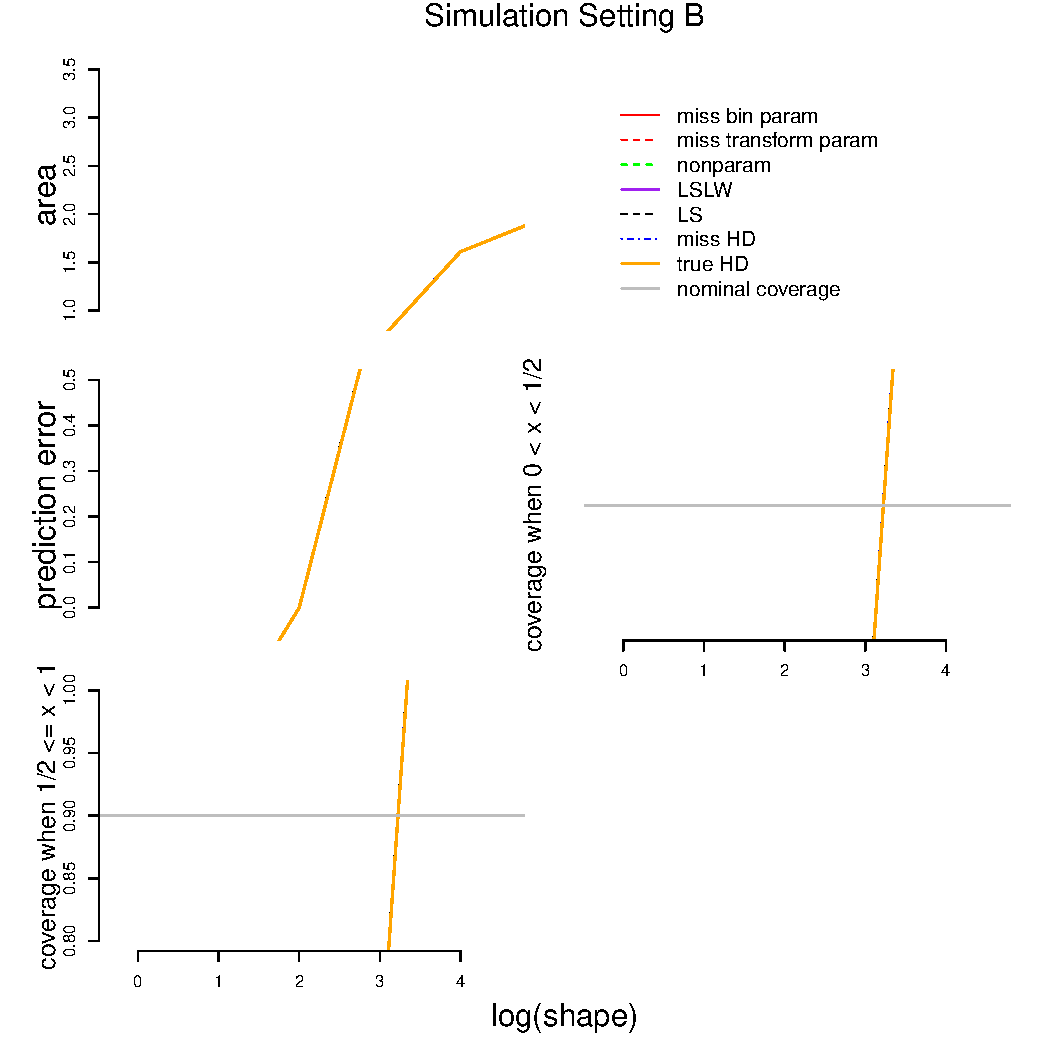
\includegraphics[width=\maxwidth]{figure/Fig-misspec-150-1} 

\end{knitrout}
\end{center}
\caption{This figure compares the performance of the 
  misspecified parametric,
  nonparametric,
  least squares, and 
  least squares locally weighted conformal prediciton region and the 
  misspecified and correctly specified highest density prediction region 
  when $n = 150$ and the number of bins equals 2.  
  The specific diagnostics used to compare these prediciton regions is the 
    area (top-left panel),
    prediction error (top-right panel), and
    the coverage probability with respect to binning (bottom row) 
    across shape parameter values.
  The average of 250 Monte Carlo samples at each shape parameter value in 
  these simulation settings form the lines that are depicted in this figure.}
\label{Fig:misspec.150}
\end{figure}



% local coverage, n = 150
\newpage
\begin{figure}[h!]
\begin{center}
\begin{knitrout}
\definecolor{shadecolor}{rgb}{0.969, 0.969, 0.969}\color{fgcolor}
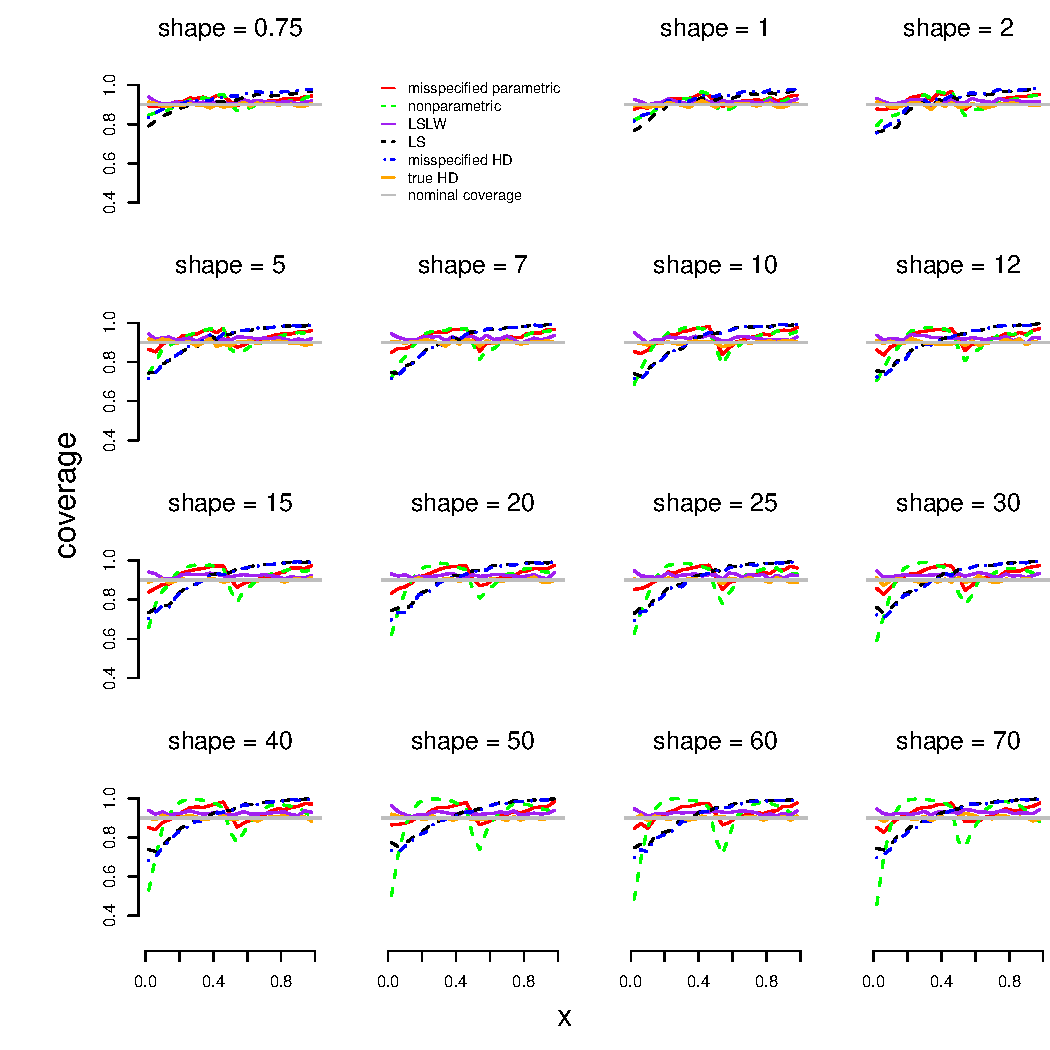
\includegraphics[width=\maxwidth]{figure/Fig-misspec-inx-150-1} 

\end{knitrout}
\end{center}
\caption{Plot of the estimated coverage probabilities of prediction regions 
  across $x$ and shape parameter values when the model is misspecified, 
  $n = 150$, and the number of bins is equal to $2$.}
\label{Fig:misspec.inx.150}
\end{figure}


% Diagnostics, n = 250
\newpage
\begin{figure}[h!]
\begin{center}
\begin{knitrout}
\definecolor{shadecolor}{rgb}{0.969, 0.969, 0.969}\color{fgcolor}
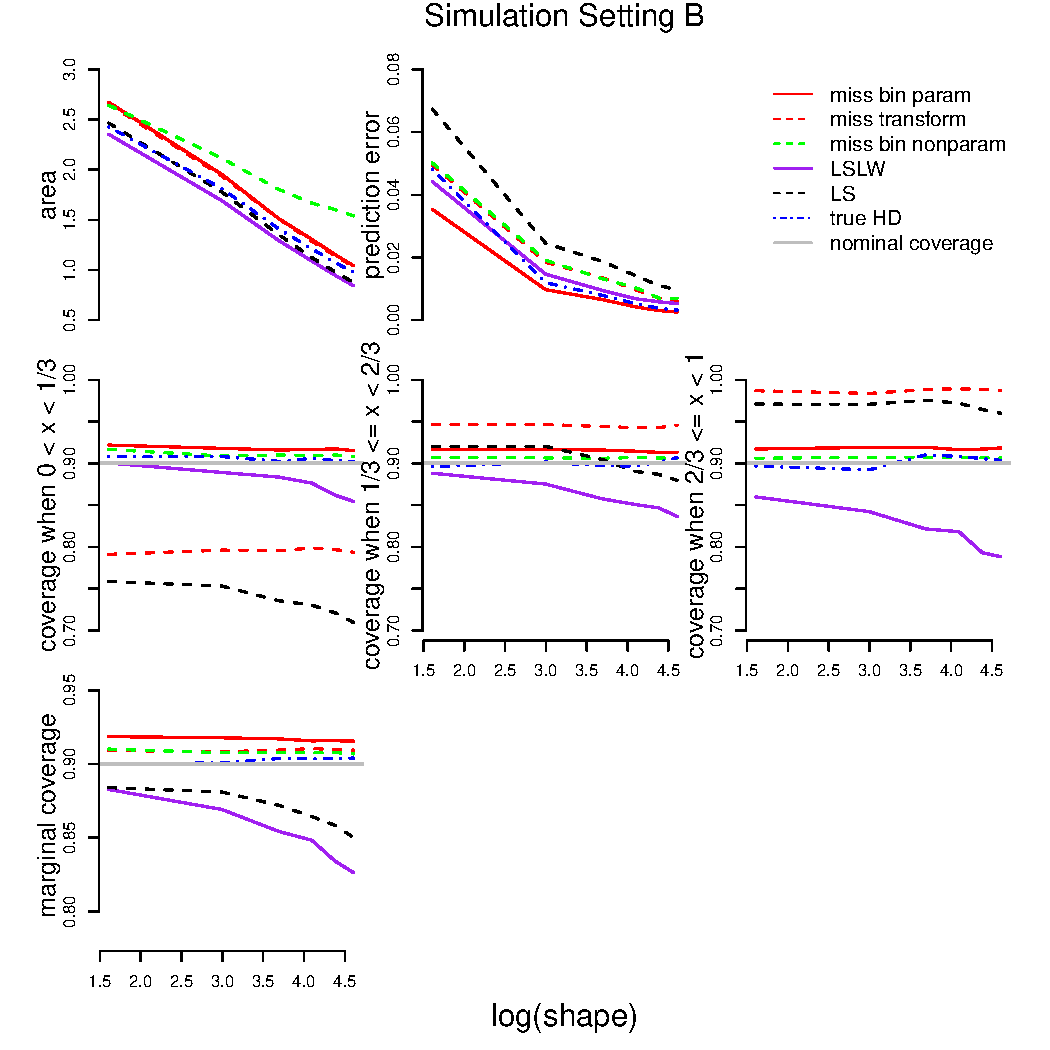
\includegraphics[width=\maxwidth]{figure/Fig-misspec-250-1} 

\end{knitrout}
\end{center}
\caption{This figure compares the performance of the 
  misspecified parametric,
  nonparametric,
  least squares, and 
  least squares locally weighted conformal prediciton region and the 
  misspecified highest density prediction region when $n = 250$ and the 
  number of bins equals 3.  
  The specific diagnostics used to compare these prediciton regions is the 
    area (top-left panel),
    prediction error (top-right panel), and
    the coverage probability with respect to binning (bottom row) 
    across shape parameter values.
  The average of 50 Monte Carlo samples at each shape parameter value in 
  these simulation settings form the lines that are depicted in this figure.}
\label{Fig:misspec.250}
\end{figure}



% local coverage, n = 250
\newpage
\begin{figure}[h!]
\begin{center}
\begin{knitrout}
\definecolor{shadecolor}{rgb}{0.969, 0.969, 0.969}\color{fgcolor}
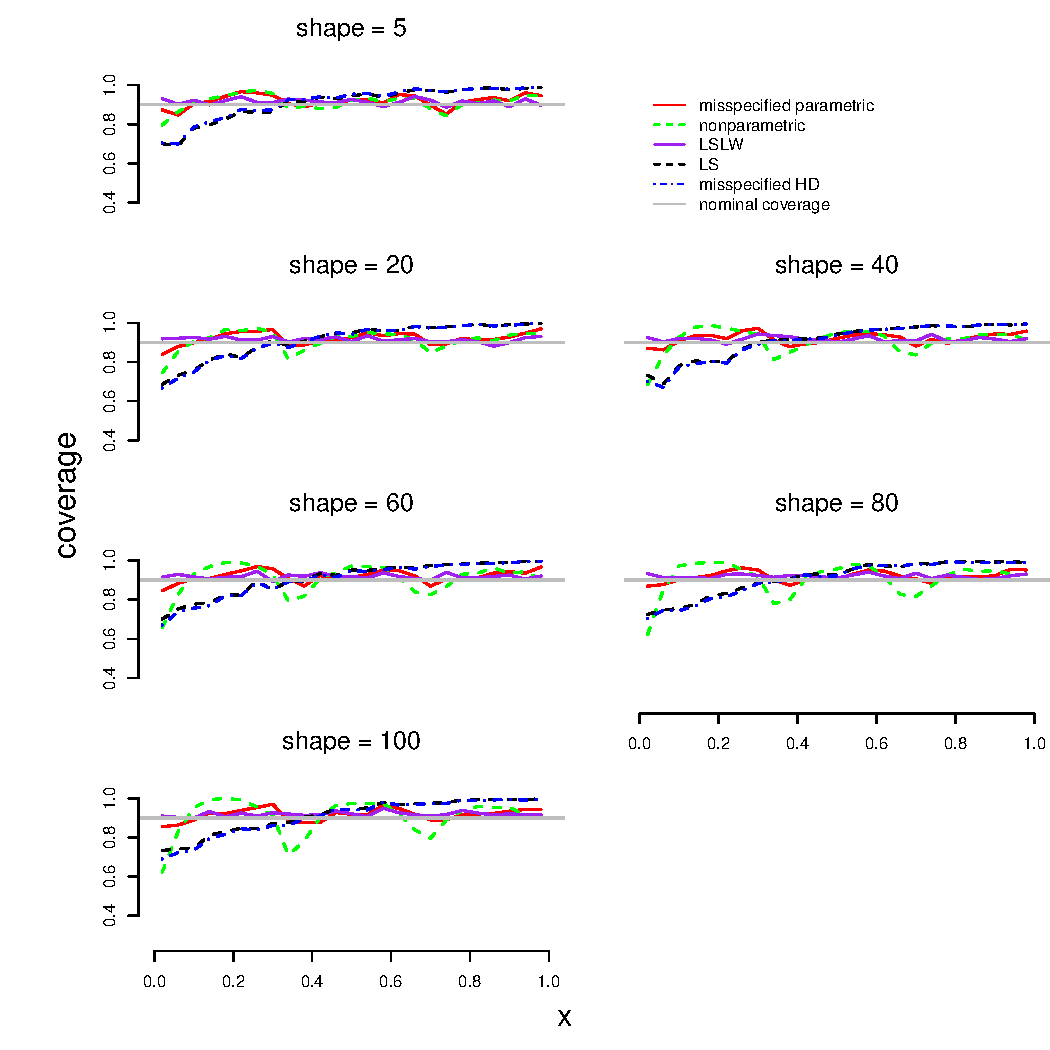
\includegraphics[width=\maxwidth]{figure/Fig-misspec-inx-250-1} 

\end{knitrout}
\end{center}
\caption{Plot of the estimated coverage probabilities of prediction regions 
  across $x$ and shape parameter values when the model is misspecified, 
  $n = 250$, and the number of bins is equal to $3$.}
\label{Fig:misspec.inx.250}
\end{figure}



% Diagnostics, n = 500
\newpage
\begin{figure}[h!]
\begin{center}
\begin{knitrout}
\definecolor{shadecolor}{rgb}{0.969, 0.969, 0.969}\color{fgcolor}
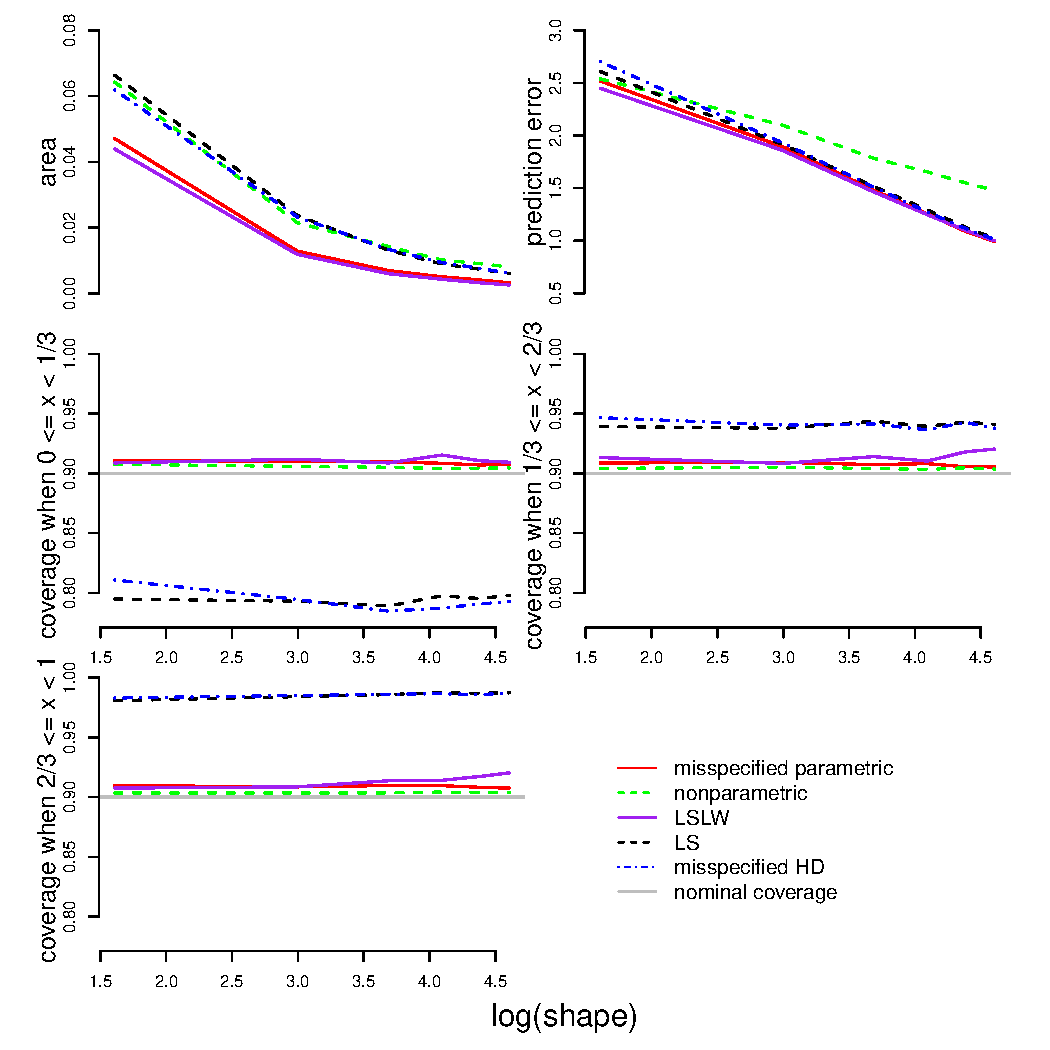
\includegraphics[width=\maxwidth]{figure/Fig-misspec-500-1} 

\end{knitrout}
\end{center}
\caption{This figure compares the performance of the 
  misspecified parametric,
  nonparametric,
  least squares, and 
  least squares locally weighted conformal prediciton region and the 
  misspecified highest density prediction region when $n = 500$ and the 
  number of bins equals 3.  
  The specific diagnostics used to compare these prediciton regions is the 
    area (top-left panel),
    prediction error (top-right panel), and
    the coverage probability with respect to binning (bottom row) 
    across shape parameter values.
  The average of 50 Monte Carlo samples at each shape parameter value in 
  these simulation settings form the lines that are depicted in this figure.}
\label{Fig:misspec.500}
\end{figure}



% local coverage, n = 500
\newpage
\begin{figure}[h!]
\begin{center}
\begin{knitrout}
\definecolor{shadecolor}{rgb}{0.969, 0.969, 0.969}\color{fgcolor}
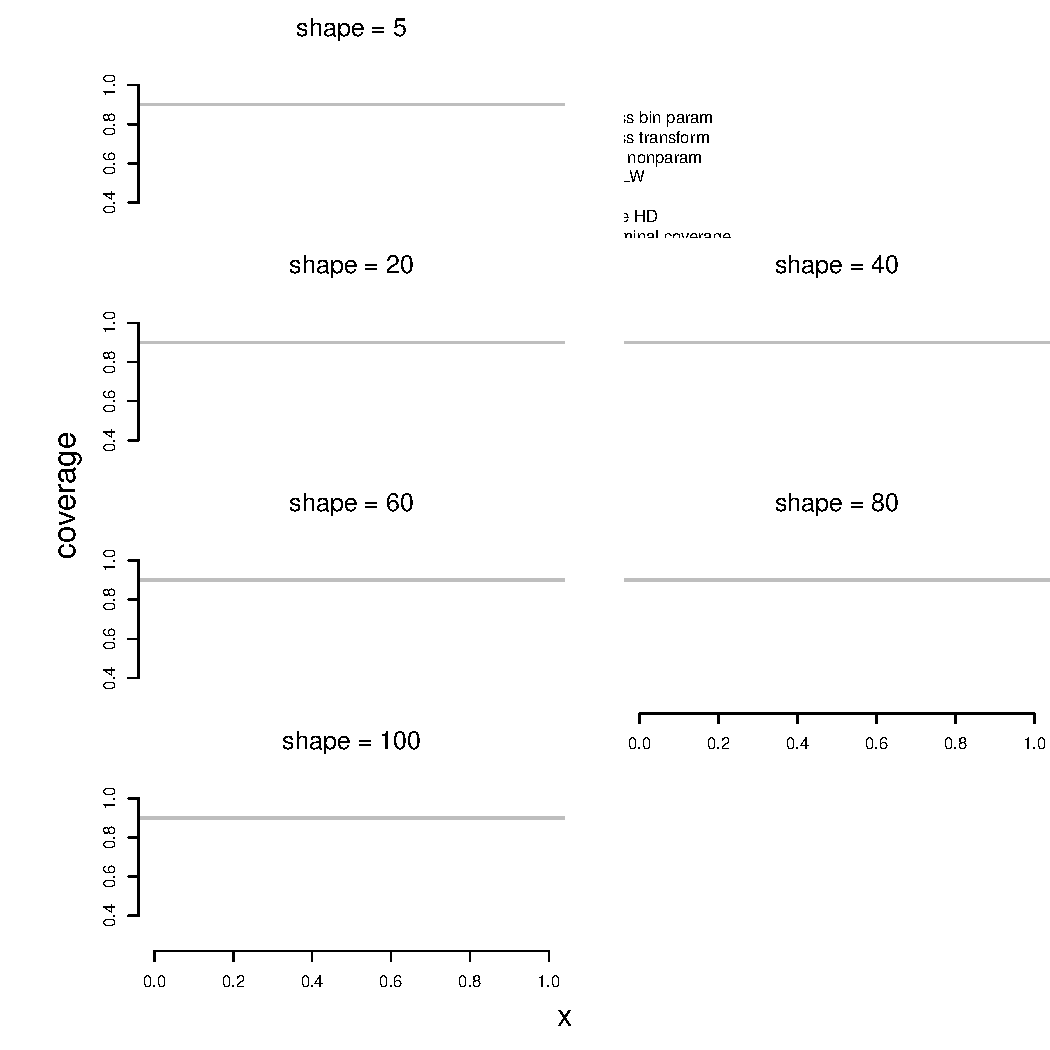
\includegraphics[width=\maxwidth]{figure/Fig-misspec-inx-500-1} 

\end{knitrout}
\end{center}
\caption{Plot of the estimated coverage probabilities of prediction regions 
  across $x$ and shape parameter values when the model is misspecified, 
  $n = 500$, and the number of bins is equal to $3$.}
\label{Fig:misspec.inx.500}
\end{figure}





\newpage
\section{Linear Regression Simulations}
\label{sec:regression}

In this Section, we compare the parametric conformal prediction 
region, the nonparametric conformal prediction region, the LSLW conformal 
prediction region, the LS conformal prediction region, and the HD prediction 
region for linear regression models with normal errors and constant variance.  
We specify that $\beta = (2, 5)^T$ and the standard deviation of the errors 
about the mean function as $\sigma = 1$.
We consider sample sizes of $n \in \{150, 250, 500\}$. 
When $n = 150$ we build the parametric and nonparametric conformal prediction 
regions using 2 bins.  When $n = 250, 500$ we build the parametric and 
nonparametric conformal prediction regions using 3 bins.  These number of bin 
choices correspond to the bin width asymptotics of \citet{lei2014distribution}. 


\subsection{Simulations}

The following function computes our diagnostic measures for the five 
prediction regions under investigation in the univariate case where data 
is generated from a Gaussian regression model, i.e. 
$Y \sim N(X'\beta, \sigma^2)$ and $X \sim U(0,1)$.

\begin{knitrout}
\definecolor{shadecolor}{rgb}{0.969, 0.969, 0.969}\color{fgcolor}\begin{kframe}
\begin{alltt}
\hlstd{regression.simulator} \hlkwb{<-} \hlkwa{function}\hlstd{(}\hlkwc{n} \hlstd{=} \hlnum{500}\hlstd{,} \hlkwc{alpha} \hlstd{=} \hlnum{0.10}\hlstd{,} \hlkwc{beta}\hlstd{,}
  \hlkwc{bins} \hlstd{=} \hlnum{3}\hlstd{,} \hlkwc{sd} \hlstd{=} \hlnum{1}\hlstd{,} \hlkwc{parametric} \hlstd{=} \hlnum{TRUE}\hlstd{,} \hlkwc{nonparametric} \hlstd{=} \hlnum{TRUE}\hlstd{,}
  \hlkwc{LS} \hlstd{=} \hlnum{TRUE}\hlstd{,} \hlkwc{LSLW} \hlstd{=} \hlnum{TRUE}\hlstd{,} \hlkwc{HD} \hlstd{=} \hlnum{TRUE}\hlstd{,} \hlkwc{cores} \hlstd{=} \hlnum{6}\hlstd{)\{}

  \hlstd{p} \hlkwb{<-} \hlstd{d} \hlkwb{<-} \hlkwd{length}\hlstd{(beta)} \hlopt{-} \hlnum{1}
  \hlstd{x} \hlkwb{<-} \hlkwd{matrix}\hlstd{(}\hlkwd{runif}\hlstd{(n),} \hlkwc{ncol} \hlstd{= p)}
  \hlstd{y} \hlkwb{<-} \hlkwd{rep}\hlstd{(}\hlnum{0}\hlstd{,n)}
  \hlstd{data} \hlkwb{<-} \hlkwa{NULL}

  \hlcom{## set up partition}
  \hlkwa{if}\hlstd{(}\hlkwd{class}\hlstd{(bins)} \hlopt{==} \hlstr{"NULL"}\hlstd{)\{}
    \hlstd{wn} \hlkwb{<-} \hlkwd{min}\hlstd{(}\hlnum{1}\hlopt{/} \hlkwd{floor}\hlstd{(}\hlnum{1} \hlopt{/} \hlstd{(}\hlkwd{log}\hlstd{(n)}\hlopt{/}\hlstd{n)}\hlopt{^}\hlstd{(}\hlnum{1}\hlopt{/}\hlstd{(d}\hlopt{+}\hlnum{3}\hlstd{))),} \hlnum{1}\hlopt{/}\hlnum{2}\hlstd{)}
    \hlstd{bins} \hlkwb{<-} \hlnum{1} \hlopt{/} \hlstd{wn}
  \hlstd{\}}

  \hlcom{## generate the data }
  \hlstd{mu} \hlkwb{<-} \hlkwd{cbind}\hlstd{(}\hlnum{1}\hlstd{, x)} \hlopt \hlstd{beta}
  \hlstd{y} \hlkwb{<-} \hlkwd{rnorm}\hlstd{(}\hlkwc{n} \hlstd{= n,} \hlkwc{mean} \hlstd{= mu,} \hlkwc{sd} \hlstd{= sd)}
  \hlstd{data} \hlkwb{<-} \hlkwd{data.frame}\hlstd{(}\hlkwc{y} \hlstd{= y,} \hlkwc{x} \hlstd{= x)}
  \hlkwd{colnames}\hlstd{(data)[}\hlnum{2}\hlopt{:}\hlstd{(p}\hlopt{+}\hlnum{1}\hlstd{)]} \hlkwb{<-} \hlkwd{paste}\hlstd{(}\hlstr{"x"}\hlstd{,} \hlnum{1}\hlopt{:}\hlstd{p,} \hlkwc{sep} \hlstd{=} \hlstr{""}\hlstd{)}

  \hlcom{## fit the linear regression model}
  \hlstd{fit} \hlkwb{<-} \hlkwd{glm}\hlstd{(y} \hlopt{~} \hlstd{x1,} \hlkwc{family} \hlstd{=} \hlstr{"gaussian"}\hlstd{,} \hlkwc{data} \hlstd{= data)}
  \hlstd{paraCI} \hlkwb{<-} \hlstd{nonparaCI} \hlkwb{<-} \hlstd{LSCI} \hlkwb{<-} \hlstd{LSLWCI} \hlkwb{<-} \hlstd{HDCI} \hlkwb{<-} \hlkwa{NULL}
  \hlstd{formula} \hlkwb{<-} \hlstd{fit}\hlopt{$}\hlstd{formula}
  \hlstd{newdata} \hlkwb{<-} \hlstd{data}
  \hlstd{respname} \hlkwb{<-} \hlkwd{all.vars}\hlstd{(formula)[}\hlnum{1}\hlstd{]}
  \hlstd{newdata} \hlkwb{<-} \hlstd{newdata[,} \hlopt{!}\hlstd{(}\hlkwd{colnames}\hlstd{(data)} \hlopt \hlstd{respname)]}
  \hlstd{newdata} \hlkwb{<-} \hlkwd{as.matrix}\hlstd{(newdata)}

  \hlcom{## obtain the prediction regions}
  \hlkwa{if}\hlstd{(parametric)\{}
    \hlstd{cpred} \hlkwb{<-} \hlkwd{conformal.glm}\hlstd{(fit,} \hlkwc{parametric} \hlstd{=} \hlnum{TRUE}\hlstd{,}
      \hlkwc{nonparametric} \hlstd{=} \hlnum{FALSE}\hlstd{,} \hlkwc{alpha} \hlstd{= alpha,}
      \hlkwc{bins} \hlstd{= bins,} \hlkwc{cores} \hlstd{= cores)}
    \hlstd{paraCI} \hlkwb{<-} \hlstd{cpred}\hlopt{$}\hlstd{paraconformal}
  \hlstd{\}}
  \hlkwa{if}\hlstd{(nonparametric)\{}
    \hlstd{cpred} \hlkwb{<-} \hlkwd{conformal.glm}\hlstd{(fit,} \hlkwc{parametric} \hlstd{=} \hlnum{FALSE}\hlstd{,}
      \hlkwc{nonparametric} \hlstd{=} \hlnum{TRUE}\hlstd{,} \hlkwc{alpha} \hlstd{= alpha,}
      \hlkwc{bins} \hlstd{= bins,} \hlkwc{cores} \hlstd{= cores)}
    \hlstd{nonparaCI} \hlkwb{<-} \hlstd{cpred}\hlopt{$}\hlstd{nonparaconformal}
  \hlstd{\}}
  \hlkwa{if}\hlstd{(LS)\{}
    \hlstd{p1.tibs} \hlkwb{<-} \hlkwd{conformal.pred}\hlstd{(}\hlkwc{x} \hlstd{= x,} \hlkwc{y} \hlstd{= y,} \hlkwc{x0} \hlstd{= x,}
      \hlkwc{train.fun} \hlstd{= train.fun,} \hlkwc{predict.fun} \hlstd{= predict.fun,}
      \hlkwc{alpha} \hlstd{= alpha)}
    \hlstd{LSCI} \hlkwb{<-} \hlkwd{cbind}\hlstd{(p1.tibs}\hlopt{$}\hlstd{lo, p1.tibs}\hlopt{$}\hlstd{up)}
  \hlstd{\}}
  \hlkwa{if}\hlstd{(LSLW)\{}
    \hlstd{regression.model} \hlkwb{<-} \hlkwd{lm}\hlstd{(y} \hlopt{~} \hlstd{x)}
    \hlstd{abs.resid} \hlkwb{<-} \hlkwd{abs}\hlstd{(regression.model}\hlopt{$}\hlstd{resid)}
    \hlstd{smooth.call} \hlkwb{<-} \hlkwd{smooth.spline}\hlstd{(x, abs.resid,}
      \hlkwc{nknots} \hlstd{=} \hlnum{10}\hlstd{)}
    \hlstd{lambda} \hlkwb{<-} \hlstd{smooth.call}\hlopt{$}\hlstd{lambda}
    \hlstd{df} \hlkwb{<-} \hlstd{smooth.call}\hlopt{$}\hlstd{df}
    \hlstd{mad.train.fun} \hlkwb{<-} \hlkwa{function}\hlstd{(}\hlkwc{x}\hlstd{,} \hlkwc{y}\hlstd{,} \hlkwc{out} \hlstd{=} \hlkwa{NULL}\hlstd{)\{}
      \hlkwd{smooth.spline}\hlstd{(x[,} \hlnum{1}\hlstd{], y,} \hlkwc{lambda} \hlstd{= lambda,}
      \hlkwc{df} \hlstd{= df,} \hlkwc{nknots} \hlstd{=} \hlnum{10}\hlstd{)}
    \hlstd{\}}
    \hlstd{p2.tibs} \hlkwb{<-} \hlkwd{conformal.pred}\hlstd{(}\hlkwc{x} \hlstd{= x,} \hlkwc{y} \hlstd{= y,} \hlkwc{x0} \hlstd{= x,}
      \hlkwc{train.fun} \hlstd{= train.fun,} \hlkwc{predict.fun} \hlstd{= predict.fun,}
      \hlkwc{mad.train.fun} \hlstd{= mad.train.fun,}
      \hlkwc{mad.predict.fun} \hlstd{= mad.predict.fun,}
      \hlkwc{alpha} \hlstd{= alpha)}
    \hlstd{LSLWCI} \hlkwb{<-} \hlkwd{cbind}\hlstd{(p2.tibs}\hlopt{$}\hlstd{lo, p2.tibs}\hlopt{$}\hlstd{up)}
  \hlstd{\}}
  \hlkwa{if}\hlstd{(HD)\{}
    \hlstd{fit} \hlkwb{=} \hlkwd{lm}\hlstd{(y} \hlopt{~} \hlstd{x,} \hlkwc{data} \hlstd{= data)}
    \hlstd{betaMLE} \hlkwb{<-} \hlkwd{coefficients}\hlstd{(fit)}
    \hlstd{sdMLE} \hlkwb{<-} \hlkwd{summary}\hlstd{(fit)}\hlopt{$}\hlstd{sigma}
    \hlstd{meanMLE} \hlkwb{<-} \hlkwd{as.numeric}\hlstd{(}\hlkwd{cbind}\hlstd{(}\hlnum{1}\hlstd{, x)} \hlopt \hlstd{betaMLE)}
    \hlstd{HDCI} \hlkwb{<-} \hlkwd{do.call}\hlstd{(rbind,} \hlkwd{lapply}\hlstd{(}\hlnum{1}\hlopt{:}\hlkwd{nrow}\hlstd{(newdata),} \hlkwa{function}\hlstd{(}\hlkwc{j}\hlstd{)\{}
      \hlkwd{hdi}\hlstd{(qnorm,} \hlnum{1} \hlopt{-} \hlstd{alpha,} \hlkwc{sd} \hlstd{= sdMLE,} \hlkwc{mean} \hlstd{= meanMLE[j])}
    \hlstd{\}))}
  \hlstd{\}}

  \hlcom{## local coverage prediction regions}
  \hlstd{output.parametric} \hlkwb{<-} \hlstd{output.nonparametric} \hlkwb{<-}
    \hlstd{output.LS} \hlkwb{<-} \hlstd{output.LSLW} \hlkwb{<-} \hlstd{output.HD} \hlkwb{<-} \hlkwd{rep}\hlstd{(}\hlnum{NA}\hlstd{, bins} \hlopt{+} \hlnum{1}\hlstd{)}
  \hlkwa{if}\hlstd{(parametric)\{}
    \hlstd{marginal.parametric} \hlkwb{<-} \hlkwd{local.coverage}\hlstd{(}\hlkwc{region} \hlstd{= paraCI,}
      \hlkwc{data} \hlstd{= data,} \hlkwc{d} \hlstd{= p,} \hlkwc{bins} \hlstd{=} \hlnum{1}\hlstd{,} \hlkwc{at.data} \hlstd{=} \hlstr{"TRUE"}\hlstd{)}
    \hlstd{local.parametric} \hlkwb{<-} \hlkwd{local.coverage}\hlstd{(}\hlkwc{region} \hlstd{= paraCI,}
      \hlkwc{data} \hlstd{= data,} \hlkwc{d} \hlstd{= p,} \hlkwc{bins} \hlstd{= bins,} \hlkwc{at.data} \hlstd{=} \hlstr{"TRUE"}\hlstd{)}
    \hlstd{local.inx.parametric} \hlkwb{<-} \hlkwd{local.coverage}\hlstd{(}\hlkwc{region} \hlstd{= paraCI,}
      \hlkwc{data} \hlstd{= data,} \hlkwc{d} \hlstd{= p,} \hlkwc{bins} \hlstd{=} \hlnum{25}\hlstd{,} \hlkwc{at.data} \hlstd{=} \hlstr{"TRUE"}\hlstd{)}
    \hlstd{output.parametric} \hlkwb{<-} \hlkwd{c}\hlstd{(marginal.parametric, local.parametric,}
      \hlstd{local.inx.parametric,}
      \hlkwd{mean}\hlstd{(}\hlkwd{apply}\hlstd{(paraCI,} \hlnum{1}\hlstd{, diff)),}
      \hlkwd{absolute.error}\hlstd{(}\hlkwc{y} \hlstd{= y,} \hlkwc{region} \hlstd{= paraCI))}
  \hlstd{\}}
  \hlkwa{if}\hlstd{(nonparametric)\{}
    \hlstd{marginal.nonparametric} \hlkwb{<-} \hlkwd{local.coverage}\hlstd{(}\hlkwc{region} \hlstd{= nonparaCI,}
      \hlkwc{nonparametric} \hlstd{=} \hlstr{"TRUE"}\hlstd{,} \hlkwc{data} \hlstd{= data,} \hlkwc{d} \hlstd{= p,} \hlkwc{bins} \hlstd{=} \hlnum{1}\hlstd{,}
      \hlkwc{at.data} \hlstd{=} \hlstr{"TRUE"}\hlstd{)}
    \hlstd{local.nonparametric} \hlkwb{<-} \hlkwd{local.coverage}\hlstd{(}\hlkwc{region} \hlstd{= nonparaCI,}
      \hlkwc{nonparametric} \hlstd{=} \hlstr{"TRUE"}\hlstd{,} \hlkwc{data} \hlstd{= data,} \hlkwc{d} \hlstd{= p,} \hlkwc{bins} \hlstd{= bins,}
      \hlkwc{at.data} \hlstd{=} \hlstr{"TRUE"}\hlstd{)}
    \hlstd{local.inx.nonparametric} \hlkwb{<-} \hlkwd{local.coverage}\hlstd{(}\hlkwc{region} \hlstd{= nonparaCI,}
      \hlkwc{nonparametric} \hlstd{=} \hlstr{"TRUE"}\hlstd{,} \hlkwc{data} \hlstd{= data,} \hlkwc{d} \hlstd{= p,} \hlkwc{bins} \hlstd{=} \hlnum{25}\hlstd{,}
      \hlkwc{at.data} \hlstd{=} \hlstr{"TRUE"}\hlstd{)}
    \hlstd{output.nonparametric} \hlkwb{<-}
      \hlkwd{c}\hlstd{(marginal.nonparametric, local.nonparametric,}
        \hlstd{local.inx.nonparametric,}
        \hlkwd{area.nonparametric}\hlstd{(nonparaCI),}
        \hlkwd{absolute.error.nonparametric}\hlstd{(}\hlkwc{data} \hlstd{= data,}
          \hlkwc{region} \hlstd{= nonparaCI))}
  \hlstd{\}}
  \hlkwa{if}\hlstd{(LS)\{}
    \hlstd{marginal.LS} \hlkwb{<-} \hlkwd{local.coverage}\hlstd{(}\hlkwc{region} \hlstd{= LSCI,}
      \hlkwc{data} \hlstd{= data,} \hlkwc{d} \hlstd{= p,} \hlkwc{bins} \hlstd{=} \hlnum{1}\hlstd{,} \hlkwc{at.data} \hlstd{=} \hlstr{"TRUE"}\hlstd{)}
    \hlstd{local.LS} \hlkwb{<-} \hlkwd{local.coverage}\hlstd{(}\hlkwc{region} \hlstd{= LSCI,}
      \hlkwc{data} \hlstd{= data,} \hlkwc{d} \hlstd{= p,} \hlkwc{bins} \hlstd{= bins,} \hlkwc{at.data} \hlstd{=} \hlstr{"TRUE"}\hlstd{)}
    \hlstd{local.inx.LS} \hlkwb{<-} \hlkwd{local.coverage}\hlstd{(}\hlkwc{region} \hlstd{= LSCI,}
      \hlkwc{data} \hlstd{= data,} \hlkwc{d} \hlstd{= p,} \hlkwc{bins} \hlstd{=} \hlnum{25}\hlstd{,} \hlkwc{at.data} \hlstd{=} \hlstr{"TRUE"}\hlstd{)}
    \hlstd{output.LS} \hlkwb{<-} \hlkwd{c}\hlstd{(marginal.LS, local.LS, local.inx.LS,}
      \hlkwd{mean}\hlstd{(}\hlkwd{apply}\hlstd{(LSCI,} \hlnum{1}\hlstd{, diff)),}
      \hlkwd{absolute.error}\hlstd{(}\hlkwc{y} \hlstd{= y,} \hlkwc{region} \hlstd{= LSCI))}
  \hlstd{\}}
  \hlkwa{if}\hlstd{(LSLW)\{}
    \hlstd{marginal.LSLW} \hlkwb{<-} \hlkwd{local.coverage}\hlstd{(}\hlkwc{region} \hlstd{= LSLWCI,}
      \hlkwc{data} \hlstd{= data,} \hlkwc{d} \hlstd{= p,} \hlkwc{bins} \hlstd{=} \hlnum{1}\hlstd{,} \hlkwc{at.data} \hlstd{=} \hlstr{"TRUE"}\hlstd{)}
    \hlstd{local.LSLW} \hlkwb{<-} \hlkwd{local.coverage}\hlstd{(}\hlkwc{region} \hlstd{= LSLWCI,}
      \hlkwc{data} \hlstd{= data,} \hlkwc{d} \hlstd{= p,} \hlkwc{bins} \hlstd{= bins,} \hlkwc{at.data} \hlstd{=} \hlstr{"TRUE"}\hlstd{)}
    \hlstd{local.inx.LSLW} \hlkwb{<-} \hlkwd{local.coverage}\hlstd{(}\hlkwc{region} \hlstd{= LSLWCI,}
      \hlkwc{data} \hlstd{= data,} \hlkwc{d} \hlstd{= p,} \hlkwc{bins} \hlstd{=} \hlnum{25}\hlstd{,} \hlkwc{at.data} \hlstd{=} \hlstr{"TRUE"}\hlstd{)}
    \hlstd{output.LSLW} \hlkwb{<-} \hlkwd{c}\hlstd{(marginal.LSLW, local.LSLW, local.inx.LSLW,}
      \hlkwd{mean}\hlstd{(}\hlkwd{apply}\hlstd{(LSLWCI,} \hlnum{1}\hlstd{, diff)),}
      \hlkwd{absolute.error}\hlstd{(}\hlkwc{y} \hlstd{= y,} \hlkwc{region} \hlstd{= LSLWCI))}
  \hlstd{\}}
  \hlkwa{if}\hlstd{(HD)\{}
    \hlstd{marginal.HD} \hlkwb{<-} \hlkwd{local.coverage}\hlstd{(}\hlkwc{region} \hlstd{= HDCI,}
      \hlkwc{data} \hlstd{= data,} \hlkwc{d} \hlstd{= p,} \hlkwc{bins} \hlstd{=} \hlnum{1}\hlstd{,} \hlkwc{at.data} \hlstd{=} \hlstr{"TRUE"}\hlstd{)}
    \hlstd{local.HD} \hlkwb{<-} \hlkwd{local.coverage}\hlstd{(}\hlkwc{region} \hlstd{= HDCI,}
      \hlkwc{data} \hlstd{= data,} \hlkwc{d} \hlstd{= p,} \hlkwc{bins} \hlstd{= bins,} \hlkwc{at.data} \hlstd{=} \hlstr{"TRUE"}\hlstd{)}
    \hlstd{local.inx.HD} \hlkwb{<-} \hlkwd{local.coverage}\hlstd{(}\hlkwc{region} \hlstd{= HDCI,}
      \hlkwc{data} \hlstd{= data,} \hlkwc{d} \hlstd{= p,} \hlkwc{bins} \hlstd{=} \hlnum{25}\hlstd{,} \hlkwc{at.data} \hlstd{=} \hlstr{"TRUE"}\hlstd{)}
    \hlstd{output.HD} \hlkwb{<-} \hlkwd{c}\hlstd{(marginal.HD, local.HD, local.inx.HD,}
      \hlkwd{mean}\hlstd{(}\hlkwd{apply}\hlstd{(HDCI,} \hlnum{1}\hlstd{, diff)),}
      \hlkwd{absolute.error}\hlstd{(}\hlkwc{y} \hlstd{= y,} \hlkwc{region} \hlstd{= HDCI))}
  \hlstd{\}}

  \hlstd{output} \hlkwb{<-} \hlkwd{list}\hlstd{(}\hlkwc{output.parametric} \hlstd{= output.parametric,}
    \hlkwc{output.nonparametric} \hlstd{= output.nonparametric,}
    \hlkwc{output.LS} \hlstd{= output.LS,}
    \hlkwc{output.LSLW} \hlstd{= output.LSLW,}
    \hlkwc{output.HD} \hlstd{= output.HD)}
  \hlstd{output}

\hlstd{\}}
\end{alltt}
\end{kframe}
\end{knitrout}


The following performs our Monte Carlo simulation of $B = 50$ iterations 
when $n = 150$.

\begin{knitrout}
\definecolor{shadecolor}{rgb}{0.969, 0.969, 0.969}\color{fgcolor}\begin{kframe}
\begin{alltt}
\hlkwd{set.seed}\hlstd{(}\hlnum{13}\hlstd{)}
\hlstd{beta} \hlkwb{<-} \hlkwd{c}\hlstd{(}\hlnum{2}\hlstd{,} \hlnum{5}\hlstd{)}
\hlstd{n} \hlkwb{<-} \hlnum{150}
\hlstd{bins} \hlkwb{<-} \hlnum{2}
\hlstd{B} \hlkwb{<-} \hlnum{50}
\hlkwd{system.time}\hlstd{(out.regression.150.2} \hlkwb{<-} \hlkwd{do.call}\hlstd{(cbind,}
  \hlkwd{lapply}\hlstd{(}\hlnum{1}\hlopt{:}\hlstd{B,} \hlkwc{FUN} \hlstd{=} \hlkwa{function}\hlstd{(}\hlkwc{j}\hlstd{)\{}
    \hlkwd{unlist}\hlstd{(}\hlkwd{regression.simulator}\hlstd{(}\hlkwc{beta} \hlstd{= beta,} \hlkwc{n} \hlstd{= n,}
      \hlkwc{bins} \hlstd{= bins))}
\hlstd{\})))}
\end{alltt}
\begin{verbatim}
##     user   system  elapsed 
## 1509.298   13.117  901.467
\end{verbatim}
\end{kframe}
\end{knitrout}

\begin{knitrout}
\definecolor{shadecolor}{rgb}{0.969, 0.969, 0.969}\color{fgcolor}\begin{kframe}
\begin{alltt}
\hlstd{regression.150.2} \hlkwb{<-} \hlkwd{cbind}\hlstd{(}
  \hlkwd{rowMeans}\hlstd{(out.regression.150.2,} \hlkwc{na.rm} \hlstd{=} \hlnum{TRUE}\hlstd{),}
  \hlkwd{apply}\hlstd{(out.regression.150.2,} \hlnum{1}\hlstd{,}
  \hlkwc{FUN} \hlstd{=} \hlkwa{function}\hlstd{(}\hlkwc{x}\hlstd{)\{}
    \hlstd{sds} \hlkwb{<-} \hlkwd{sd}\hlstd{(x,} \hlkwc{na.rm} \hlstd{=} \hlnum{TRUE}\hlstd{)}
    \hlstd{lengths} \hlkwb{<-} \hlkwd{length}\hlstd{(}\hlkwd{which}\hlstd{(}\hlopt{!}\hlkwd{is.na}\hlstd{(x)))}
    \hlstd{sds} \hlopt{/} \hlkwd{sqrt}\hlstd{(lengths)}
  \hlstd{\}))}
\end{alltt}
\end{kframe}
\end{knitrout}

The following performs our Monte Carlo simulation of $B = 50$ iterations 
when $n = 150$.

\begin{knitrout}
\definecolor{shadecolor}{rgb}{0.969, 0.969, 0.969}\color{fgcolor}\begin{kframe}
\begin{alltt}
\hlstd{n} \hlkwb{<-} \hlnum{250}
\hlstd{bins} \hlkwb{<-} \hlnum{3}
\hlkwd{system.time}\hlstd{(out.regression.250.3} \hlkwb{<-} \hlkwd{do.call}\hlstd{(cbind,}
  \hlkwd{lapply}\hlstd{(}\hlnum{1}\hlopt{:}\hlstd{B,} \hlkwc{FUN} \hlstd{=} \hlkwa{function}\hlstd{(}\hlkwc{j}\hlstd{)\{}
    \hlkwd{unlist}\hlstd{(}\hlkwd{regression.simulator}\hlstd{(}\hlkwc{beta} \hlstd{= beta,} \hlkwc{n} \hlstd{= n,}
      \hlkwc{bins} \hlstd{= bins))}
\hlstd{\})))}
\end{alltt}
\begin{verbatim}
##     user   system  elapsed 
## 2945.050   18.113 1846.314
\end{verbatim}
\end{kframe}
\end{knitrout}

\begin{knitrout}
\definecolor{shadecolor}{rgb}{0.969, 0.969, 0.969}\color{fgcolor}\begin{kframe}
\begin{alltt}
\hlstd{regression.250.3} \hlkwb{<-} \hlkwd{cbind}\hlstd{(}
  \hlkwd{rowMeans}\hlstd{(out.regression.250.3,} \hlkwc{na.rm} \hlstd{=} \hlnum{TRUE}\hlstd{),}
  \hlkwd{apply}\hlstd{(out.regression.250.3,} \hlnum{1}\hlstd{,}
  \hlkwc{FUN} \hlstd{=} \hlkwa{function}\hlstd{(}\hlkwc{x}\hlstd{)\{}
    \hlstd{sds} \hlkwb{<-} \hlkwd{sd}\hlstd{(x,} \hlkwc{na.rm} \hlstd{=} \hlnum{TRUE}\hlstd{)}
    \hlstd{lengths} \hlkwb{<-} \hlkwd{length}\hlstd{(}\hlkwd{which}\hlstd{(}\hlopt{!}\hlkwd{is.na}\hlstd{(x)))}
    \hlstd{sds} \hlopt{/} \hlkwd{sqrt}\hlstd{(lengths)}
  \hlstd{\}))}
\end{alltt}
\end{kframe}
\end{knitrout}

The following performs our Monte Carlo simulation of $B = 50$ iterations 
when $n = 500$.

\begin{knitrout}
\definecolor{shadecolor}{rgb}{0.969, 0.969, 0.969}\color{fgcolor}\begin{kframe}
\begin{alltt}
\hlstd{n} \hlkwb{<-} \hlnum{500}
\hlkwd{system.time}\hlstd{(out.regression.500.3} \hlkwb{<-} \hlkwd{do.call}\hlstd{(cbind,}
  \hlkwd{lapply}\hlstd{(}\hlnum{1}\hlopt{:}\hlstd{B,} \hlkwc{FUN} \hlstd{=} \hlkwa{function}\hlstd{(}\hlkwc{j}\hlstd{)\{}
    \hlkwd{unlist}\hlstd{(}\hlkwd{regression.simulator}\hlstd{(}\hlkwc{beta} \hlstd{= beta,} \hlkwc{n} \hlstd{= n,}
      \hlkwc{bins} \hlstd{= bins))}
\hlstd{\})))}
\end{alltt}
\begin{verbatim}
##     user   system  elapsed 
## 7285.245   19.752 4517.354
\end{verbatim}
\end{kframe}
\end{knitrout}

\begin{knitrout}
\definecolor{shadecolor}{rgb}{0.969, 0.969, 0.969}\color{fgcolor}\begin{kframe}
\begin{alltt}
\hlstd{regression.500.3} \hlkwb{<-} \hlkwd{cbind}\hlstd{(}
  \hlkwd{rowMeans}\hlstd{(out.regression.500.3,} \hlkwc{na.rm} \hlstd{=} \hlnum{TRUE}\hlstd{),}
  \hlkwd{apply}\hlstd{(out.regression.500.3,} \hlnum{1}\hlstd{,}
  \hlkwc{FUN} \hlstd{=} \hlkwa{function}\hlstd{(}\hlkwc{x}\hlstd{)\{}
    \hlstd{sds} \hlkwb{<-} \hlkwd{sd}\hlstd{(x,} \hlkwc{na.rm} \hlstd{=} \hlnum{TRUE}\hlstd{)}
    \hlstd{lengths} \hlkwb{<-} \hlkwd{length}\hlstd{(}\hlkwd{which}\hlstd{(}\hlopt{!}\hlkwd{is.na}\hlstd{(x)))}
    \hlstd{sds} \hlopt{/} \hlkwd{sqrt}\hlstd{(lengths)}
  \hlstd{\}))}
\end{alltt}
\end{kframe}
\end{knitrout}



\subsection{Results}

Results form our simulations are depicted in 
Table~\ref{Tab:regression-results} and Figure~\ref{Fig:regresion.inx}.  
This table and figure depicts the estimatated area, prediction 
error, and local coverage probabilities for all five considered prediction 
regions. 

In these simulations, errors about the estimated mean function are symmetric 
and homogeneous across the support.  We therefore expect for the LS and LSLW 
conformal prediction regions to perform nearly as well as the oracle HD 
prediction region.  These prediction regions also exhibit finite-sample 
marginal validity, local validity with respect to binning, and near 
conditional validity across the support.  The parametric conformal prediction 
region is similar to the LS and LSLW conformal prediciton regions and the HD 
prediction region in area, prediction error, finite-sample coverage 
properties, and appearance.  However, the parametric conformal prediciton 
region is slightly larger and gives more conservative coverage that these 
other prediction regions.  The nonparametric conformal prediciton region 
is larger and gives larger prediciton errors than the other prediciton 
regions.  It also appears to not visually fit the data well while the others 
do as seen in Section~\ref{sec:regressionplots}.





\begin{table}[h!]
\tiny
\begin{center}
\begin{tabular}{llccccc}
  & & parametric conformal & nonparametric conformal & LS conformal & 
    LSLW conformal & HD region \\ 
  $n = 150$
    & marginal coverage &
  $0.922 \; (0.0007)$ & 
  $0.916 \; (0.001)$ & 
  $0.913 \; (0.001)$ & 
  $0.918  (0.0011)$ & 
  $0.904 \; (0.0023)$ \\
    & local coverage when $0 < x < 1/2$ & 
  $0.922 \; (0.0011)$ & 
  $0.916 \; (0.0014)$ & 
  $0.912 \; (0.0035)$ & 
  $0.921 \; (0.0029)$ & 
  $0.903 \; (0.0042)$ \\
    & local coverage when $1/2 \leq x < 1$ & 
  $0.922 \; (0.001)$ & 
  $0.916 \; (0.0016)$ & 
  $0.914 \; (0.0036)$ & 
  $0.915 \; (0.003)$ & 
  $0.904 \; (0.0036)$ \\
    & area &
  $3.521 \; (0.0366)$ & 
  $4.258 \; (0.0466)$ & 
  $3.361 \; (0.0291)$ & 
  $3.385 \; (0.0322)$ & 
  $3.28 \; (0.0263)$ \\
    & prediction error &
  $0.021 \; (0.0011)$ & 
  $0.033 \; (0.0023)$ & 
  $0.027 \; (0.0015)$ & 
  $0.023 \; (0.0013)$ & 
  $0.03 \; (0.0013)$ \\
  \hline
  $n = 250$  
    & marginal coverage &
  $0.918 \; (0.0006)$ & 
  $0.915 \; (0.0007)$ & 
  $0.908 \; (0.0006)$ & 
  $0.911 \; (0.0007)$ & 
  $0.901 \; (0.0014)$ \\
    & local coverage when $0 < x < 1/3$ & 
  $0.919 \; (0.001)$ & 
  $0.915 \; (0.0014)$ & 
  $0.91 \; (0.0036)$ & 
  $0.912 \; (0.0034)$ & 
  $0.905 \; (0.0039)$ \\
    & local coverage when $1/3 \leq x < 2/3$ & 
  $0.917 \; (0.0007)$ & 
  $0.917 \; (0.0014)$ & 
  $0.912 \; (0.0035)$ & 
  $0.913 \; (0.0028)$ & 
  $0.907 \; (0.0039)$ \\
    & local coverage when $2/3 \leq x < 1$ &
  $0.918 \; (0.001)$ & 
  $0.915 \; (0.0015)$ & 
  $0.904 \; (0.0042)$ & 
  $0.907 \; (0.0032)$ & 
  $0.893 \; (0.0046)$ \\
    & area & 
  $3.518 \; (0.0291)$ & 
  $3.822 \; (0.0338)$ & 
  $3.36 \; (0.0233)$ & 
  $3.363 \; (0.0261)$ & 
  $3.296 \; (0.0218)$ \\
    & prediction error & 
  $0.021 \; (0.0013)$ & 
  $0.028 \; (0.0017)$ & 
  $0.027 \; (0.0013)$ & 
  $0.025 \; (0.0013)$ & 
  $0.029 \; (0.0013)$ \\
  \hline
  $n = 500$
    & marginal coverage & 
  $0.908 \; (0.0002)$ & 
  $0.907 \; (0.0004)$ & 
  $0.905 \; (0.0005)$ & 
  $0.906 \; (0.0005)$ & 
  $0.903 \; (0.0013)$ \\
    & local coverage when $0 < x < 1/3$ & 
  $0.909 \; (0.0004)$ & 
  $0.907 \; (0.0008)$ & 
  $0.907 \; (0.0032)$ & 
  $0.906 \; (0.0025)$ & 
  $0.905 \; (0.0034)$ \\
    & local coverage when $1/3 \leq x < 2/3$ & 
  $0.908 \; (0.0004)$ & 
  $0.906 \; (0.0006)$ & 
  $0.907 \; (0.0026)$ & 
  $0.906 \; (0.0021)$ & 
  $0.907 \; (0.0029)$ \\
    & local coverage when $2/3 \leq x < 1$ & 
  $0.909 \; (0.0005)$ & 
  $0.908 \; (0.0007)$ & 
  $0.901 \; (0.0024)$ & 
  $0.905 \; (0.0021)$ & 
  $0.898 \; (0.0028)$ \\
    & area & 
  $3.369 \; (0.0211)$ & 
  $3.715 \; (0.0187)$ & 
  $3.305 \; (0.0206)$ & 
  $3.314 \; (0.0202)$ & 
  $3.287 \; (0.0169)$ \\
    & prediction error & 
  $0.026 \; (0.0013)$ & 
  $0.033 \; (0.0013)$ & 
  $0.029 \; (0.0014)$ & 
  $0.028 \; (0.0014)$ & 
  $0.03 \; (0.0011)$ 
\end{tabular}
\end{center}
\caption{Diagnostics for conformal prediction regions for linear regression 
  models with normal errors and constant variance.  Local and marginal 
  coverage properties, areas, and prediction errors are presented for the 
    parametric conformal prediction region (third column),
    nonparametric conformal prediction region (fourth column),
    LS conformal prediction region (fifth column), 
    LSLW conformal prediction region (sixth column), and 
    HD prediction region (seventh column). Standard errors are in parentheses.}
\label{Tab:regression-results}
\end{table}





\newpage
\begin{figure}[h!]
\begin{center}
\begin{knitrout}
\definecolor{shadecolor}{rgb}{0.969, 0.969, 0.969}\color{fgcolor}
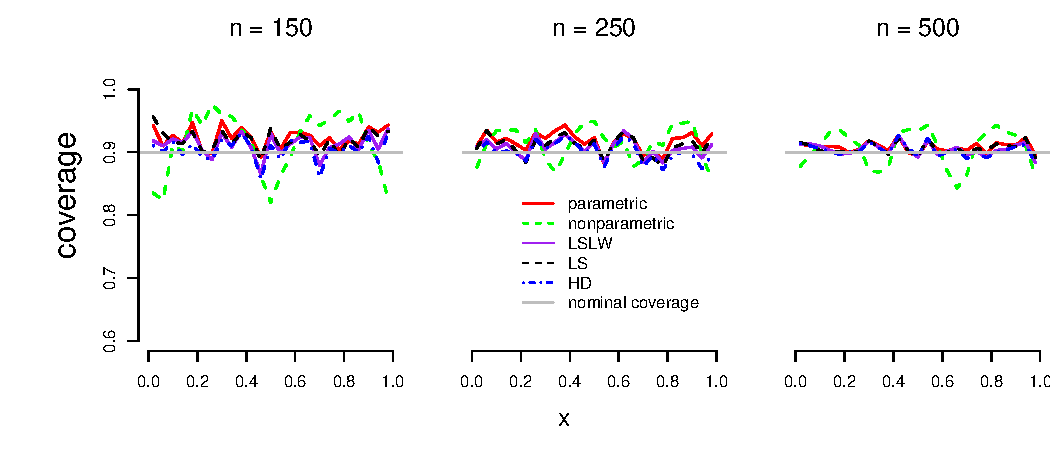
\includegraphics[width=\maxwidth]{figure/Fig-regression-inx-500-1} 

\end{knitrout}
\end{center}
\caption{Plot of the estimated coverage probabilities of prediction regions 
  across $x$ and sample sizes.}
\label{Fig:regresion.inx}
\end{figure}






\newpage
\section{Example plots of prediction regions}
\label{sec:plotsofregions}

In this section we construct prediction regions corresponding to the 
simulations and results in Sections~\ref{sec:Gamma} through 
\ref{sec:regressionplots}.  In Gamma analyses we generate a dataset for each 
shape parameter considered with $n = 150$ and in regression analyses we 
generate a dataset for all sample sizes considered.  For each of these datasets 
we depict the parametric, nonparametric, LS, LSLW conformal prediction regions 
over the observed data to visually assess the appropriateness of each 
prediction region.  The findings from these figures are consistent with the 
findings from our numerical diagnostics.  
The parametric conformal prediction region gives visually natural bounds for 
the observed data when the model is correctly specified in small to moderate 
sample sizes and is appropriate when the model is misspecified. 
The LSLW conformal prediction region gives visually natural bounds for the 
observed data when the model is correctly specified, is appropriate under mild 
model misspecification, and is ill-fitting in settings where deviations about 
an estimated mean function are clearly not symmetric.
The nonparametric conformal prediction region is coarse and is larger than 
necessary when the mean function is steep relative to its variability.  
The LS conformal prediction performs well when deviations about the estimated 
mean function are symmetirc and is sensitive to mild departures from that 
setting.  This prediciton region is seen to provide overcoverage 
(undercoverage) in regions of the predictor space where variability about the 
estimated mean function is relatively small (large).



\newpage
\begin{figure}[h!]
\begin{center}
\begin{knitrout}
\definecolor{shadecolor}{rgb}{0.969, 0.969, 0.969}\color{fgcolor}
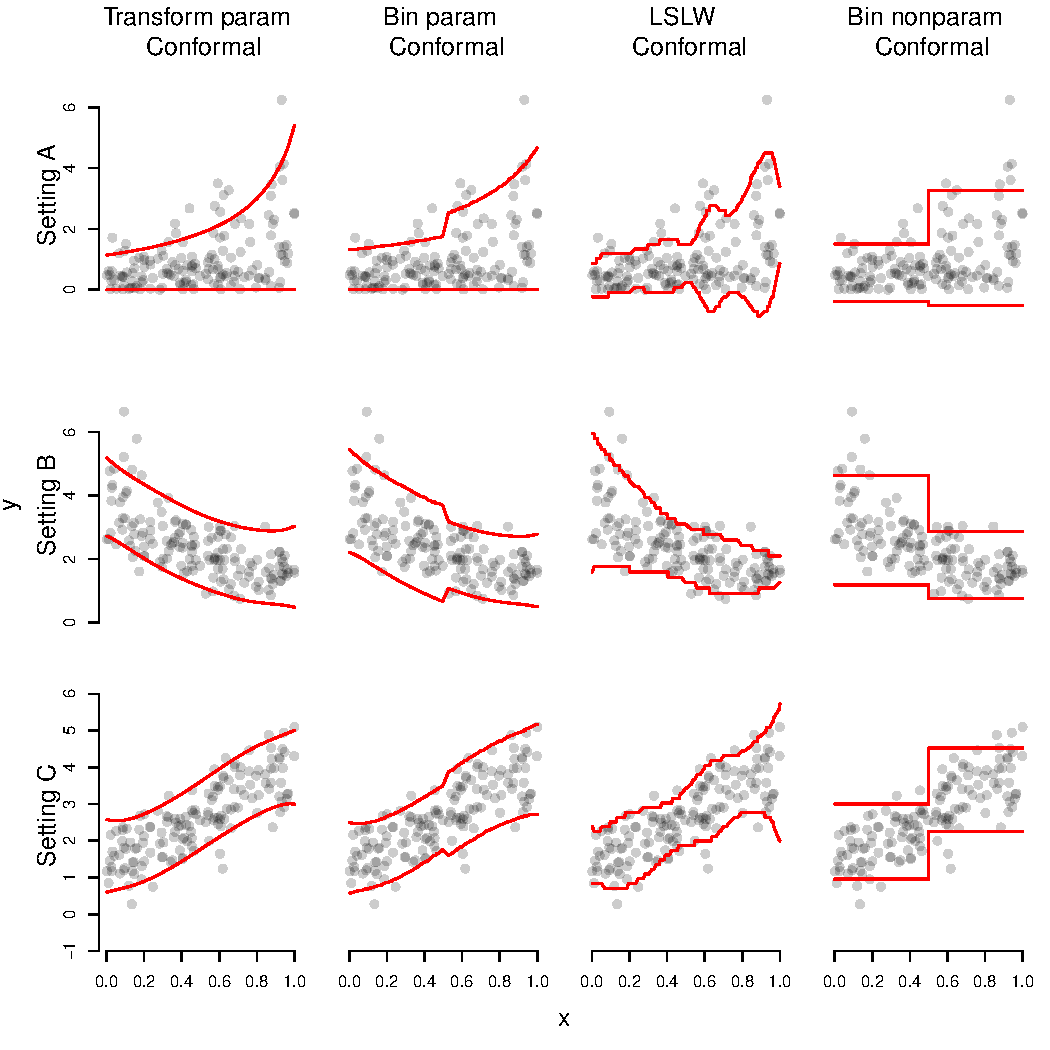
\includegraphics[width=\maxwidth]{figure/conformal-plots-1} 

\end{knitrout}
\end{center}
\caption{The depiction of conformal prediction regions when $n = 150$ that 
  appears in \citet{eck2019conformal}.  The rows display conformal prediction 
  regions across simulation settings.  The columns display the different 
  conformal prediction regions.  The top, middle, and bottom rows correspond 
  to simulation setting a with shape parameter equal to 1, simulation setting 
  b with shape parameter equal to 10, and simulation setting c respectively.  
  The first column displays the parametric conformal prediction region which 
  is misspecified in row 2, the second column displays the least squares 
  locally weighted conformal prediction region, the third column displays the 
  nonparametric conformal prediction region, and the fourth column displays 
  the least squares conformal prediction region.}
\label{conformal-plots}
\end{figure}











\newpage
\subsection{Plots corresponding to Section~\ref{sec:Gamma}}
\label{sec:gammaplots}

%Plot of conformal prediciton regions in sim setting A when n = 150
\begin{figure}[h!]
\begin{center}
\begin{knitrout}
\definecolor{shadecolor}{rgb}{0.969, 0.969, 0.969}\color{fgcolor}
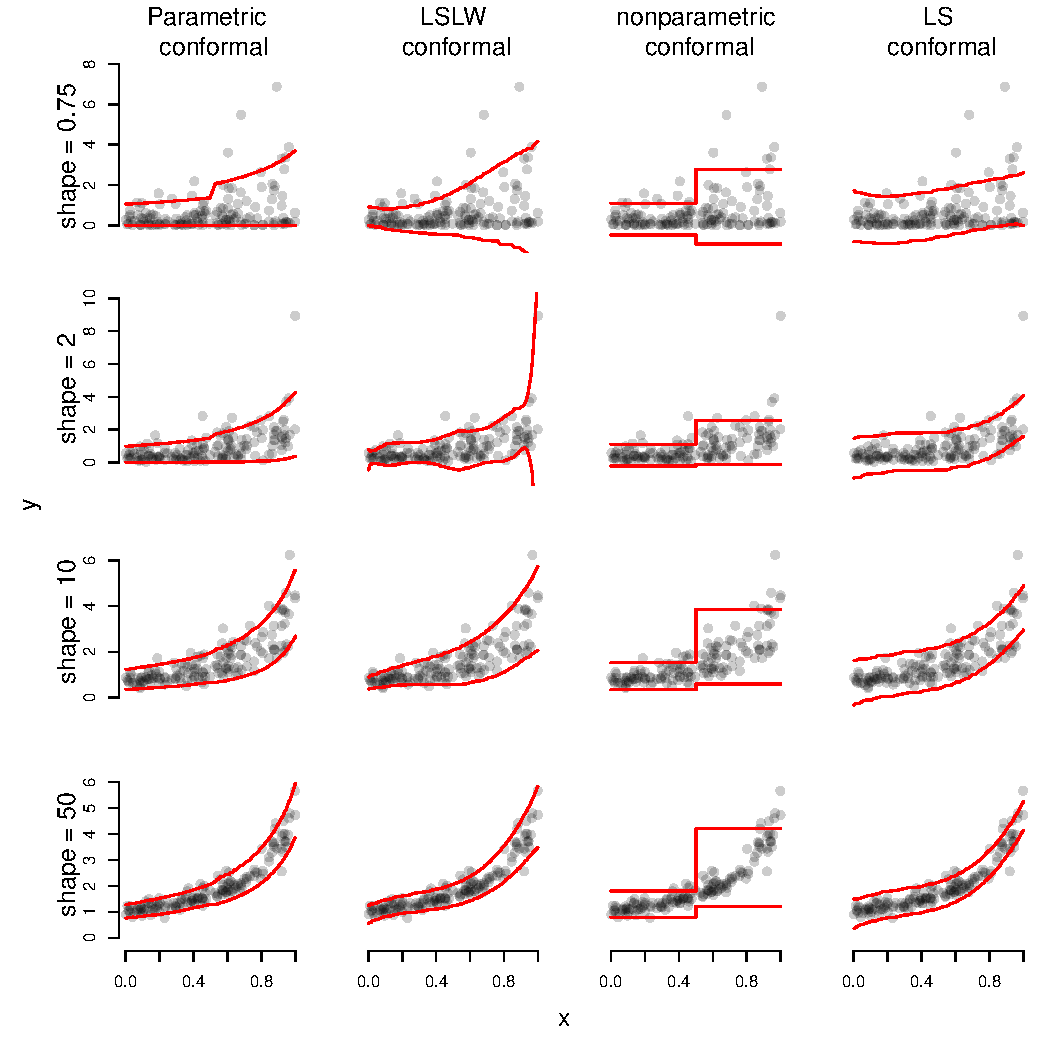
\includegraphics[width=\maxwidth]{figure/conformal-plots-A-150-1} 

\end{knitrout}
\end{center}
\caption{The depiction of conformal prediction regions under simulation 
  setting A when $n = 150$ and the number of bins equals 2.
}
\label{conformal-plots-A-150}
\end{figure}











\newpage
%Plot of conformal prediciton regions in sim setting A when n = 250
\begin{figure}[h!]
\begin{center}
\begin{knitrout}
\definecolor{shadecolor}{rgb}{0.969, 0.969, 0.969}\color{fgcolor}
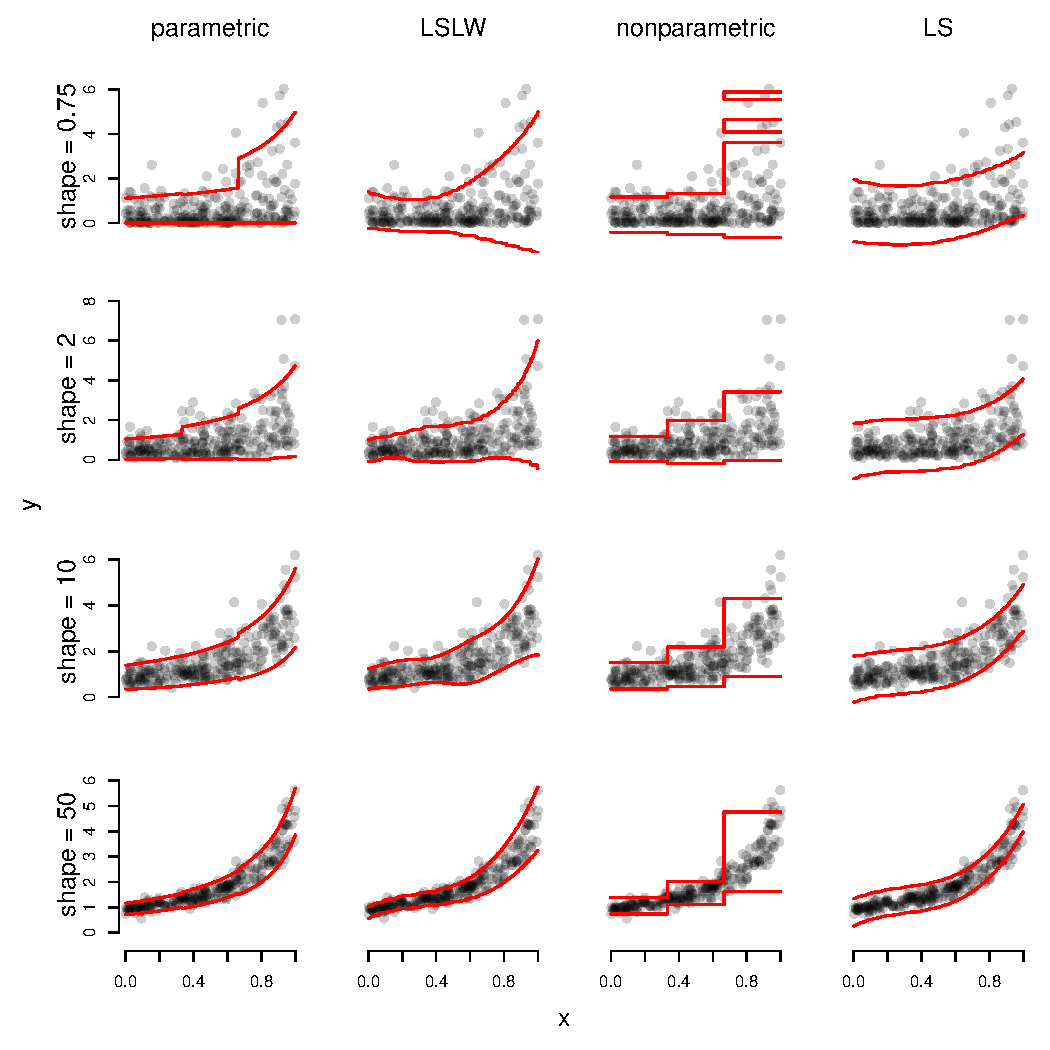
\includegraphics[width=\maxwidth]{figure/conformal-plots-A-250-1} 

\end{knitrout}
\end{center}
\caption{The depiction of conformal prediction regions under simulation 
  setting A when $n = 250$ and the number of bins equals 3.
}
\label{conformal-plots-A-250}
\end{figure}








\newpage
%Plot of conformal prediciton regions in sim setting A when n = 500
\begin{figure}[h!]
\begin{center}
\begin{knitrout}
\definecolor{shadecolor}{rgb}{0.969, 0.969, 0.969}\color{fgcolor}
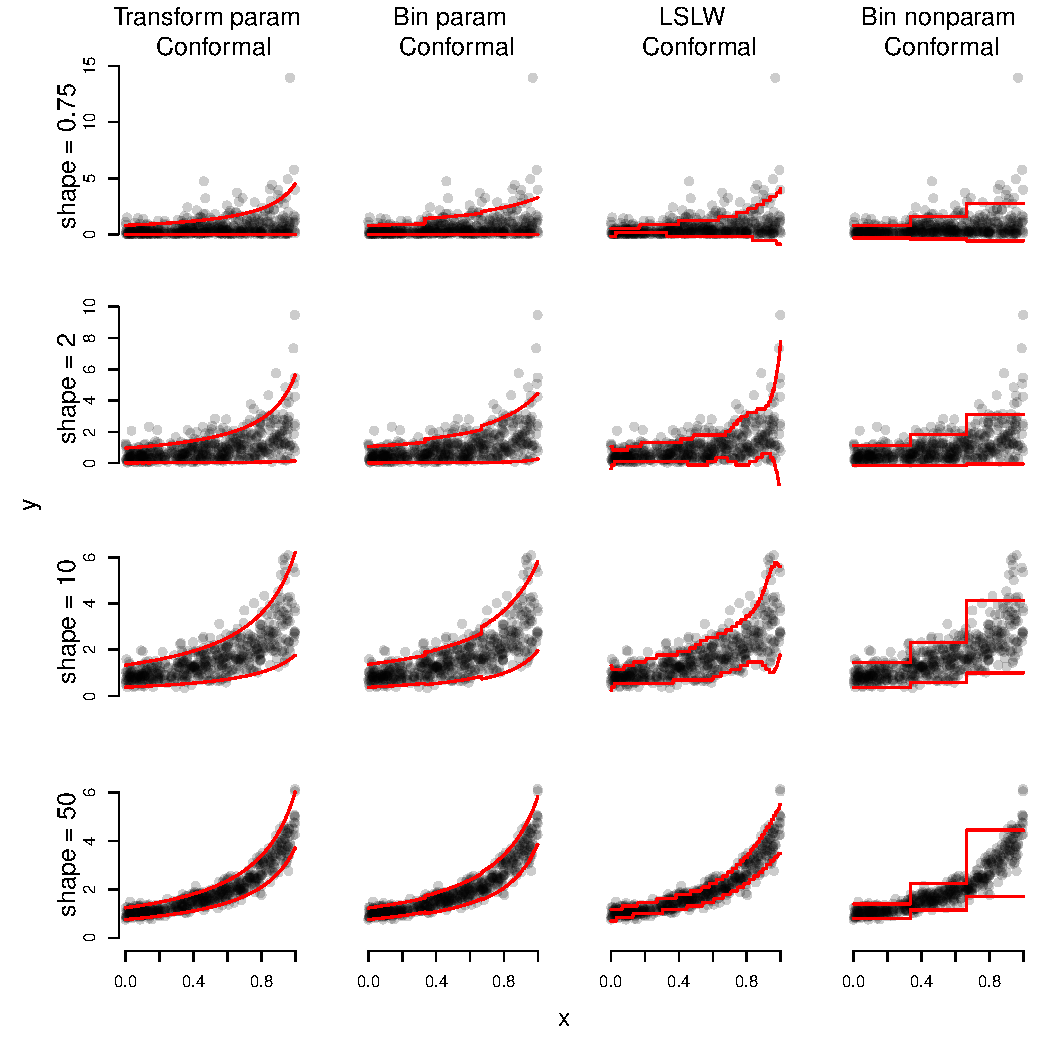
\includegraphics[width=\maxwidth]{figure/conformal-plots-A-500-1} 

\end{knitrout}
\end{center}
\caption{The depiction of conformal prediction regions under simulation 
  setting A when $n = 500$ and the number of bins equals 3.
}
\label{conformal-plots-A-500}
\end{figure}







\newpage
\subsection{Plots corresponding to Section~\ref{sec:misspec}}
\label{sec:misspecplots}


%Plot of conformal prediciton regions in sim setting B when n = 150
\begin{figure}[h!]
\begin{center}
\begin{knitrout}
\definecolor{shadecolor}{rgb}{0.969, 0.969, 0.969}\color{fgcolor}
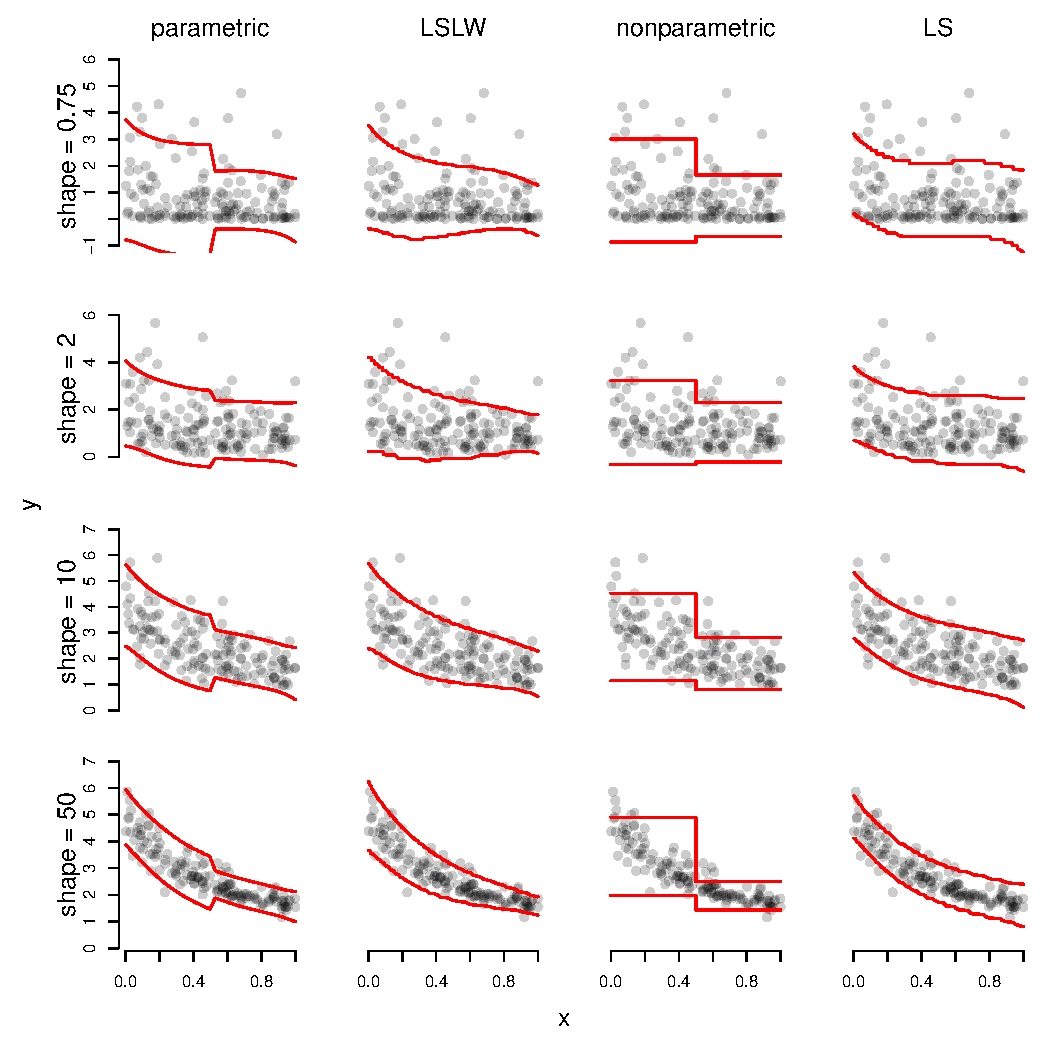
\includegraphics[width=\maxwidth]{figure/conformal-plots-B-150-1} 

\end{knitrout}
\end{center}
\caption{The depiction of conformal prediction regions under simulation 
  setting B when $n = 150$ and the number of bins equals 2.
}
\label{conformal-plots-B-150}
\end{figure}










\newpage
%Plot of conformal prediciton regions in sim setting B when n = 250
\begin{figure}[h!]
\begin{center}
\begin{knitrout}
\definecolor{shadecolor}{rgb}{0.969, 0.969, 0.969}\color{fgcolor}
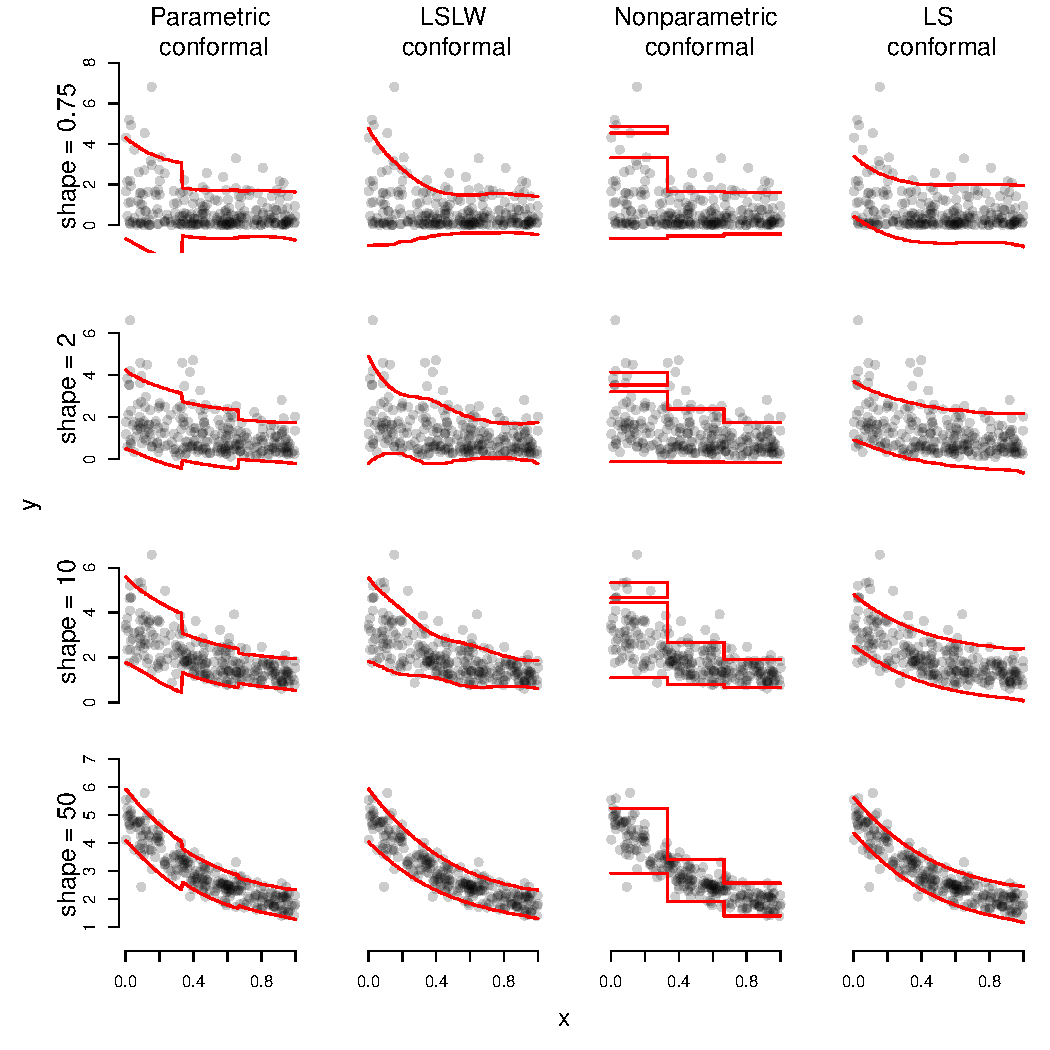
\includegraphics[width=\maxwidth]{figure/conformal-plots-B-250-1} 

\end{knitrout}
\end{center}
\caption{The depiction of conformal prediction regions under simulation 
  setting B when $n = 250$ and the number of bins equals 3.
}
\label{conformal-plots-B-250}
\end{figure}









\newpage
%Plot of conformal prediciton regions in sim setting B when n = 500
\begin{figure}[h!]
\begin{center}
\begin{knitrout}
\definecolor{shadecolor}{rgb}{0.969, 0.969, 0.969}\color{fgcolor}
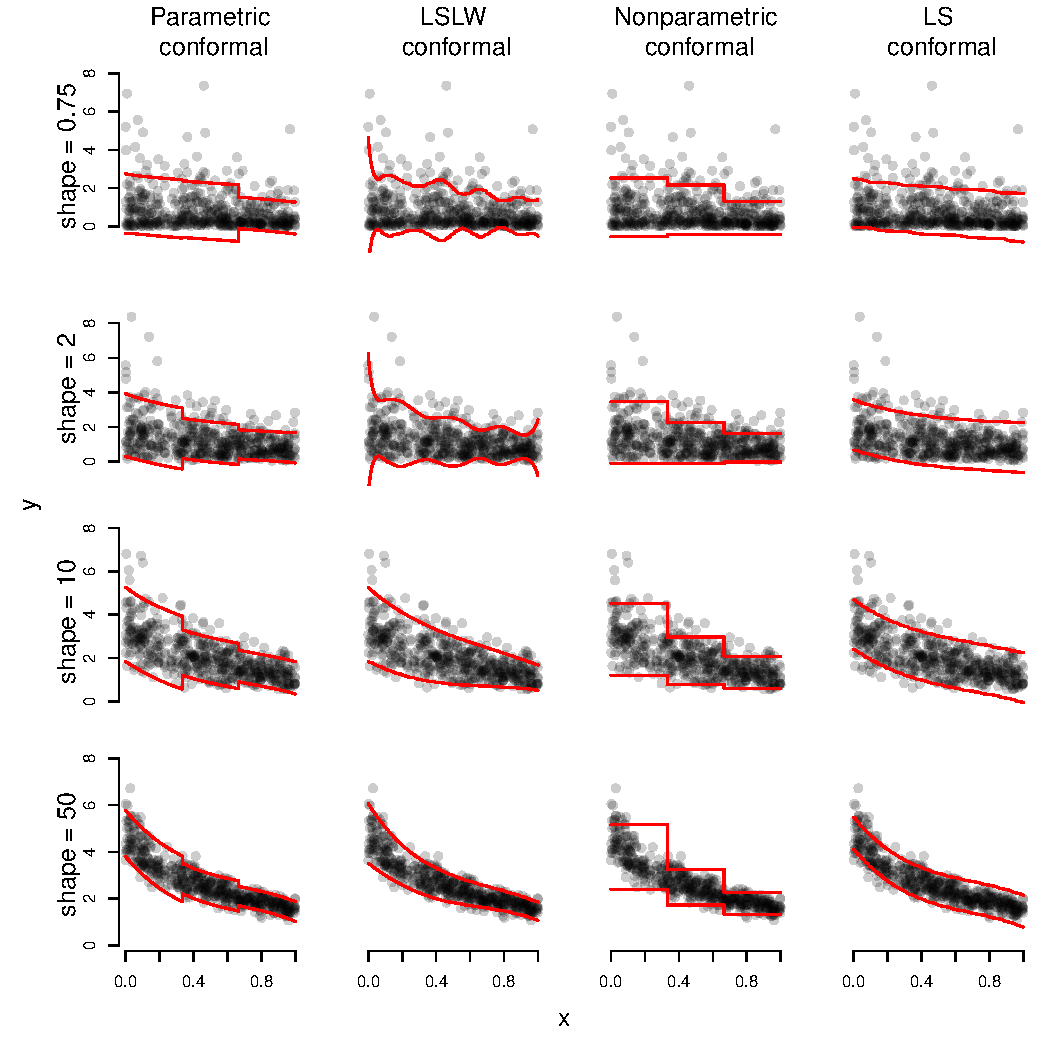
\includegraphics[width=\maxwidth]{figure/conformal-plots-B-500-1} 

\end{knitrout}
\end{center}
\caption{The depiction of conformal prediction regions under simulation 
  setting B when $n = 500$ and the number of bins equals 3.
}
\label{conformal-plots-B-500}
\end{figure}









\newpage
\subsection{Plots corresponding to Section~\ref{sec:regression}}
\label{sec:regressionplots}

%Plot of conformal prediciton regions in sim setting C
\begin{figure}[h!]
\begin{center}
\begin{knitrout}
\definecolor{shadecolor}{rgb}{0.969, 0.969, 0.969}\color{fgcolor}
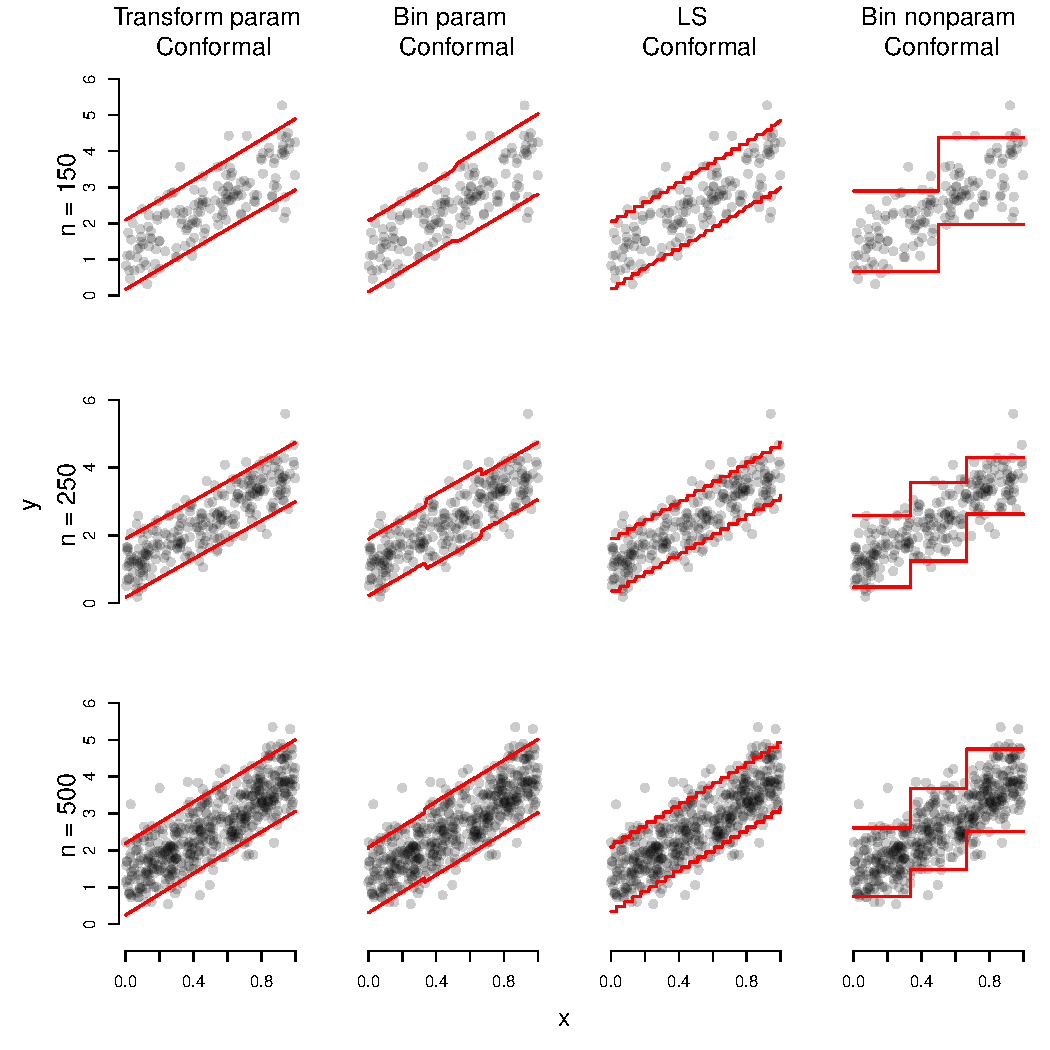
\includegraphics[width=\maxwidth]{figure/conformal-plots-C-1} 

\end{knitrout}
\end{center}
\caption{The depiction of conformal prediction regions under simulation 
  setting C.
}
\label{conformal-plots-C}
\end{figure}


















\section{Creating this Document}
The purpose of this document is to provide a completely reproducible 
exploration and motivation of conformal prediction. All of the R code 
presented in this document (or the corresponding .Rnw file) is run when 
this document is compiled using the linux terminal.

This document is created from its source file 
\texttt{supplement-conformal.Rnw} using \texttt{knitr} and the 
\texttt{pdflatex} command in the linux terminal. The \texttt{knitr} R package 
needs to be installed before this document can be compiled. Open R and install 
this package if you have not previously done so. To compile this document in 
the linux terminal, enter the command 
\vspace{0.25cm}\\
\texttt{Rscript -e "library(knitr); knit('supplement-conformal.Rnw')"} 
\vspace{0.25cm}\\
This produces the LaTex .tex file with the name 
\texttt{supplement-conformal.tex}. To get a corresponding .pdf file, enter 
the command
\vspace{0.25cm}\\
\texttt{pdflatex supplement-conformal.tex} 
\vspace{0.25cm}\\
You may want to run the previous command twice in order to get labels and 
references right.

\bibliographystyle{plainnat}

\bibliography{conformalsources}

\end{document}

